%!TEX program = pdflatex
%!TEX encoding = UTF-8 Unicode

\documentclass[defaultstyle,10pt,master]{01.thesis}
% Helvetica is a similar font to Arial, with small differences.

\usepackage[default,scale=0.95]{opensans} %% Alternatively
\usepackage[T1]{fontenc}


%% Packages
%!TEX root = ../tese.tex
%!TEX encoding = UTF-8 Unicode
% PACKAGE babel:
% ---------------
% The 'babel' package may correct some hyphenisation issues of latex. 
% However in most situations it is not required.
\usepackage[english]{babel}
\usepackage[utf8]{inputenc}
\usepackage{setspace}
% \usepackage[latin1]{inputenc}
% PACKAGE fontenc:
% -----------------
% chooses T1-fonts and allows correct automatic hyphenation.

% Package ulem.
\usepackage{ulem} % Allows the use of other text emphatizer commands
\normalem %defines \emph{} to italic, instead of underline. 
\raggedbottom %declaration makes all pages the height of the text on that page. No extra vertical space is added. The \flushbottom declaration makes all text pages the same height, adding extra vertical space when necessary to fill out the page.

% PACKAGE date time:
% -----------------
% Lets you alter the format of the date that \today returns.
\usepackage{datetime}
\newdateformat{todaythesis}{%
\monthname[\THEMONTH]  \THEYEAR}

% PACKAGE latexsym:
% -----------------
% Defines additional latex symbols. May be required for thesis with many math symbols.
\usepackage{latexsym}

% PACKAGE amsmath, amsthm, amssymb, amsfonts:
% -------------------------------------------
% This package is typically required. Among many other things it adds the possibility
% to put symbols in bold by using \boldsymbol (not \mathbf); defines additional 
% fonts and symbols; adds the \eqref command for citing equations. I prefer the style
% "(x.xx)" for referering to an equation than to use "equation x.xx".
\usepackage{amsmath, amsthm, amssymb, amsfonts, amsbsy}

%support to alpha enumerations
\usepackage{enumitem}


% PACKAGE multirow, colortbl, longtable:
% ---------------------------------------
% These packages are most usefull for advanced tables. The first allows to join rows 
% throuhg the command \multirow which works similarly with the command \multicolumn
% The second package allows to color the table (both foreground and background)
% The third package is only required when tables extend beyond the length of one page;
% with compatibilities with the tabular environment. The last allow the definitions of landscape pages, allowing the use of a different orientation for wider graphics or tables. See package documentation to see the implementation.
\usepackage{multirow}
\usepackage{colortbl}
\usepackage{tabularx}
\usepackage{tabulary}
\usepackage{pdflscape}
\usepackage{longtable}
\usepackage{tabu}
\usepackage{multicol} %support two column layout 

% PACKAGE graphics, epsfig, subfigure, caption:
% ---------------------------------------------
% Packages for figures... well you will certainly need these packages, with the exception
% of the 'caption' package. This only allows to define extra caption options.
% Notice that subfigure allows to place figures within figures with its own caption. It
% should be avoided to create an eps file with subfigures. That will mean that you won't be 
% able to reference those subfigures. Instead create an EPS file (the only graphics format supported
% by latex) for each of the subfigures and then use the command \subfigure (see below).
\usepackage{graphics}
\usepackage{graphicx, epstopdf}
\usepackage{epsfig}
\usepackage{subfig}
\usepackage{caption}
\usepackage{dcolumn}
\usepackage{bm}
\usepackage{booktabs}
\usepackage{rotating}
\usepackage{multirow}
\usepackage{listings}

%Color on table
\usepackage[table]{xcolor}


%Marks on table
\usepackage{pifont}% http://ctan.org/pkg/pifont
\newcommand{\cmark}{\ding{51}}%
\newcommand{\xmark}{\ding{55}}%



\usepackage{courier}
\usepackage{amsmath}

%\usepackage{minted}
\usepackage{mathtext}
\usepackage{framed}
\definecolor{shadecolor}{rgb}{1,1,1}
\usepackage{color} 
\usepackage{array}
%\usepackage{etex}
\usepackage{wrapfig}
\usepackage{chngpage} % allows for temporary adjustment of side margins
%\usepackage{booktabs}
%\usepackage{float}

\usepackage{array}
\newcolumntype{C}[1]{>{\centering\arraybackslash}m{#1}}

%Allows Highlight for teacher
\usepackage{soulutf8}

%Use \FloatBarrier to prevent floats (images) from crossing the sections
\usepackage[section]{placeins}

\newcolumntype{x}[1]{>{\centering\let\newline\\\arraybackslash\hspace{0pt}}p{#1}}

\definecolor{lightgray}{gray}{0.9}
\colorlet{punct}{red!60!black}
\definecolor{background}{HTML}{EEEEEE}
\definecolor{delim}{RGB}{20,105,176}
\colorlet{numb}{magenta!60!black}

\newcommand{\tab}[1]{\hspace{.2\textwidth}\rlap{#1}}


\newcommand{\us}{\,$\mu$$s$\xspace} 
\newcommand{\ms}{\,$ms$\xspace} 


%-----------------------------------------------------------
\newenvironment{dedication}
  {\clearpage           % we want a new page
   \thispagestyle{empty}% no header and footer
   \vspace*{\stretch{3}}% some space at the top 
   \itshape             % the text is in italics
   \raggedleft          % flush to the right margin
  }
  {\par % end the paragraph
   \vspace{\stretch{1}} % space at bottom is three times that at the top
   \clearpage           % finish off the page
  }


\lstdefinelanguage{json}{
    basicstyle=\normalfont\ttfamily,
    numbers=left,
    numberstyle=\scriptsize,
    stepnumber=1,
    numbersep=8pt,
    showstringspaces=false,
    breaklines=true,
    frame=lines,
    backgroundcolor=\color{background},
    literate=
     *{0}{{{\color{numb}0}}}{1}
      {1}{{{\color{numb}1}}}{1}
      {2}{{{\color{numb}2}}}{1}
      {3}{{{\color{numb}3}}}{1}
      {4}{{{\color{numb}4}}}{1}
      {5}{{{\color{numb}5}}}{1}
      {6}{{{\color{numb}6}}}{1}
      {7}{{{\color{numb}7}}}{1}
      {8}{{{\color{numb}8}}}{1}
      {9}{{{\color{numb}9}}}{1}
      {:}{{{\color{punct}{:}}}}{1}
      {,}{{{\color{punct}{,}}}}{1}
      {\{}{{{\color{delim}{\{}}}}{1}
      {\}}{{{\color{delim}{\}}}}}{1}
      {[}{{{\color{delim}{[}}}}{1}
      {]}{{{\color{delim}{]}}}}{1},
}

%-----------------------------------------------------------

\lstdefinelanguage{Protobuff}{
  keywords={message,enum},
  keywordstyle=\bfseries,
  morekeywords={[2]{required,repeated,optional}},
  keywordstyle={[2]{\textit}},
  identifierstyle=\color{black},
  sensitive=false,
  comment=[l]{//},
  morecomment=[s]{/*}{*/},
  commentstyle=\color{black}\ttfamily,
  stringstyle=\color{black}\ttfamily,
  morestring=[b]',
  morestring=[b]"
}




\usepackage[font=small,labelfont=bf,textfont=normalfont]{caption}

% PACKAGE algorithmic, algorithm
% ------------------------------
% These packages are required if you need to describe an algorithm.
%\usepackage{algorithmic}
%\usepackage[chapter]{algorithm}
\usepackage[linesnumbered,ruled,noend,noline]{algorithm2e}
\usepackage{algpseudocode}
\setlength{\algomargin}{2em}
\newcommand*\Letv[2]{$#1 \gets$ #2}
\newcommand*\Let[2]{#1 $\gets$ #2}

% PACKAGE natbib/cite
% -------------------
% The two packages are not compatible, and you should use one of the two. Notice however that the
% IEEE BiBTeX stylesheet is imcompatible with the natbib package. If using the IEEE format, use the 
% cite package instead
\usepackage[square,numbers,sort&compress]{natbib}
%\usepackage{cite}

% PACKAGE acronyum
% -----------------
% This package is most useful for acronyms. The package guarantees that all acronyms definitions are 
% given at the first usage. IMPORTANT: do not use acronyms in titles/captions; otherwise the definition 
% will appear on the table of contents.
\usepackage[printonlyused]{acronym}
\usepackage[titletoc,title,header]{appendix}
\usepackage[noauto]{chappg}

% PACKAGE extra_functions VER COMO DEVE SER
% -----------------
% My Personal package: defines the following commands:
% \fancychapter{chaptername) -> Prints a fancier chapter (you can also use the fancychapter package for this)
% \hline{width} -> use for a replacement of the \hline command
% \Mark1, \Mark2, \Mark3, ...
\usepackage{00.extra_functions}

\definecolor{grey}{rgb}{0.97,0.97,0.97}


% PACKAGE hyperref
% -----------------
% Set links for references and citations in document
% Some MiKTeX distributions have faulty PDF creators in which case this package will not work correctly
% Long live Linux :D
\usepackage[plainpages=false]{hyperref}
\hypersetup{
             colorlinks=false,
             citecolor=red,
             breaklinks=true,
             bookmarksnumbered=true,
             bookmarksopen=true,
             pdftitle={Thesis Title},
             pdfauthor={Author Name},
             pdfsubject={Master Thesis in Biomedical Engineering},
             pdfcreator={Document Creator Name},
             pdfkeywords={Template, Latex, Thesis}}
\usepackage{float}
%\usepackage[final]{00.listofsymbols}
\usepackage{00.symlist}

% Inserted by Jackie
\usepackage{fixltx2e} % for super- and subscripts
\usepackage[final]{pdfpages}

% Set paragraph counter to alphanumeric mode       
\renewcommand{\theparagraph}{\Alph{paragraph}}               

\newcommand{\figref}[1]{Figure \ref{#1}}
\newcommand{\equationref}[1]{Equation (\ref{#1})}
\newcommand{\tableref}[1]{Table (\ref{#1})}

\newcommand{\textreg}{$\textsuperscript{\textregistered}$}

% Inserted by Jackie
\makeatletter
\renewcommand\paragraph{\@startsection{paragraph}{0}{\z@}%
                       {-12\p@ \@plus -4\p@ \@minus -4\p@}%
                       {8\p@ \@plus 4\p@ \@minus 4\p@}%
                       {\normalfont\normalsize\bfseries\boldmath
                        \rightskip=\z@ \@plus 8em\pretolerance=10000}}
                        \makeatother       
\renewcommand{\theparagraph}{}        

% Big O notation
\renewcommand{\O}[1]{$\mathcal{O}(#1)$}
\newcolumntype{R}[1]{>{\raggedleft\let\newline\\\arraybackslash\hspace{0pt}}m{#1}}

\newcommand{\LONG}[1]{}

%% Page formatting
\hoffset 0in
\voffset 0in

%Alternative set of page geometry
%\oddsidemargin 0.71cm
%\evensidemargin 0.04cm
%\marginparsep 0in
%\topmargin -0.25cm
%\textwidth 15cm
%\textheight 23.5cm

\usepackage[top=2.5cm, bottom=2.5cm, inner=2.9cm, outer=2.5cm]{geometry}

\usepackage{fancyhdr}
\pagestyle{fancy}
\renewcommand{\chaptermark}[1]{\markboth{\thechapter.\ #1}{}}
\renewcommand{\sectionmark}[1]{\markright{\thesection\ #1}}
\fancyhf{} 
%\fancyhead[LE]{\bfseries\nouppercase{\leftmark}}
%\fancyhead[RO]{\bfseries\nouppercase{\rightmark}}
\fancyfoot[LE,RO]{\bfseries\small\thepage}
\renewcommand{\headrulewidth}{0.0pt}
\renewcommand{\footrulewidth}{0.0pt}
\addtolength{\headheight}{2pt} % make space for the rule
\fancypagestyle{plain}{% Used in Chapter titles
   \fancyhead{} % get rid of headers
   \renewcommand{\headrulewidth}{0pt} % and the line
   \renewcommand{\footrulewidth}{0pt}
   \fancyfoot[LE,RO]{\bfseries\small\thepage}
}

\fancypagestyle{begin}{%
   \fancyhead{}
   \renewcommand{\headrulewidth}{0pt}
   \renewcommand{\footrulewidth}{0pt}
   \fancyfoot[LE,RO]{\bfseries\small\thepage}
}
\fancypagestyle{document}{%
	\fancyhf{} 
	\fancyhead[LE]{\bfseries\nouppercase{\leftmark}}
	\fancyhead[RO]{\bfseries\nouppercase{\rightmark}}
	\fancyfoot[LE,RO]{\bfseries\small\thepage}
	%\renewcommand{\headrulewidth}{0pt}
	%\renewcommand{\footrulewidth}{0pt}
	\addtolength{\headheight}{2pt} % make space for the rule
}
\fancypagestyle{documentsimple}{%
	\fancyhf{}
	\fancyfoot[LE,RO]{\bfseries\small\thepage}
	%\renewcommand{\headrulewidth}{0pt}
	%\renewcommand{\footrulewidth}{0pt}
	\addtolength{\headheight}{2pt} % make space for the rule
}
\setcounter{secnumdepth} {5}
\setcounter{tocdepth} {2}
%\renewcommand{\thesubsubsection}{\thesubsection.\Alph{subsubsection}}

%\renewcommand{\subfigtopskip}{0.3 cm}
%\renewcommand{\subfigbottomskip}{0.2 cm}
%\renewcommand{\subfigcapskip}{0.3 cm}
%\renewcommand{\subfigcapmargin}{0.2 cm}

\graphicspath{{Figures/}}

% Define cover page fonts
%
%         encoding     family       series      shape
%  \usefont{T1}     {phv}=helvetica  {b}=bold    {n}=normal
%                   {ptm}=times      {m}=normal  {sl}=slanted
%                                                {it}=italic
% see more examples at
% http://julien.coron.free.fr/languages/latex/fonts/
%
\def\FontLn{% 16 pt normal
  \usefont{T1}{phv}{m}{n}\fontsize{16pt}{16pt}\selectfont}
\def\FontLb{% 16 pt bold
  \usefont{T1}{phv}{b}{n}\fontsize{16pt}{16pt}\selectfont}
\def\FontMn{% 14 pt normal
  \usefont{T1}{phv}{m}{n}\fontsize{14pt}{14pt}\selectfont}
\def\FontMb{% 14 pt bold
  \usefont{T1}{phv}{b}{n}\fontsize{14pt}{14pt}\selectfont}
\def\FontSn{% 12 pt normal
  \usefont{T1}{phv}{m}{n}\fontsize{12pt}{12pt}\selectfont}

%\addtolength{\topmargin}{-2mm}
%\addtolength{\topskip}{-2mm}
%\addtolength{\textheight}{+5mm}
%\addtolength{\textwidth}{+5mm}



\newdateformat{monthYearDate}{\monthname[\THEMONTH] \THEYEAR}

\begin{document}
\pagestyle{begin}

\raggedbottom
\pagenumbering{arabic}


%!TEX root = ../../tese.tex
%!TEX encoding = UTF-8 Unicode
\setcounter{page}{1} \pagenumbering{Alph}

% Add PDF bookmark 
\pdfbookmark[0]{Title}{Title}

\thispagestyle{empty}
\begin{flushleft} ~\\ \vspace{-10mm} \hspace{-9mm}  
\includegraphics[width=50mm]{Cover/LogoIST-new} 
\\ \vspace{80mm}
\begin{centering}
{\FontLb Recovery from Security Intrusions in Cloud Computing} \\
\vspace{2.8cm}
{\FontMb Dário Fernando Rodrigues Nascimento} \\
\vspace{2cm}
{\FontSn Thesis to obtain the Master Degree in} \\
\vspace{0.3cm}
{\FontLb Telecommunications and Computers Engineering}\\ 
\vspace{1.1cm}
{\FontSn Supervisor: Prof. Dr. Miguel Pupo Correia}\\
\vspace{1.1cm}
{\FontMb Examination Committee} \\
\vspace{0.3cm}
{\FontSn %
\renewcommand{\arraystretch}{1.5} % General space between rows (1 standard)
\begin{tabular}{ll}
Chairperson: & Prof.  Dr. Paulo Jorge Pires Ferreira \\ 
Supervisor: & Prof. Dr. Miguel Pupo Correia \\ 
Members of the Committee: & Prof. Dr. Nuno Manuel Ribeiro Preguiça
\end{tabular}}\\
\vspace{15mm}
{\FontMb May 2015} \\
\end{centering}
\let\thepage\relax
\end{flushleft}
\pagebreak


\clearpage
% Since I am using double sided pages, the second page should be white.
% Remember that when delivering the dissertation, IST requires for the cover to appear twice.

\thispagestyle{empty}
\cleardoublepage

\setcounter{page}{1} \pagenumbering{roman}

\baselineskip 18pt  
%!TEX root = ../../tese.tex
%!TEX encoding = UTF-8 Unicode
\raggedbottom
\pdfbookmark{Acknowledgements}{Acknowledgements}
\begin{acknowledgments}
\begin{doublespace}

This dissertation owes its existence from the proposal made by my advisor, Miguel Pupo Correia, who supports me since the beginning, allowed me to do this thesis often remotely and gave me many great ideas and enthusiasm.\\
Thanks to the creators of my Family (my grand-parents), specially to my grand-father José Paulo Nascimento who became an orphan when he was young and humbly worked hard on civil construction, agriculture and aviculture to create a big happy and reliable family. Thanks for your great inspiration.
Equal thanks go to my parents for supporting all my crazy life decisions, great education and happy family environment. Thanks to my sister and cousins for so much fun and good moments.
Francisco Malheiro, Mário Malheiro, Teresa Alves, Sara Alves, Paula Alves, André Santos, Joana Malheiro, Pedro Alves my hearth friends since ever.\\
Pedro Gomes, Marcella Monteiro (special gratefulness for many English texts reviews), Rui Caldas, Tânia Rodrigues, Vanessa Silva my crazy and great friends since high-school. Gonçalo Pestana (great mate in Aalto), Artur Balanuta, David Dias, Gonçalo Carito, Francisco Esteves, Tiago Freire, Rita Raimundo, Bruno Mercês my closest friends in Instituto Superior Técnico.\\
Special thanks to Maike Marzendorfer for being always by my side sharing best and worst moments of my life.\\
Thanks go as well to all my friends from Board of European Students of Technology (BEST), Erasmus, Filarmónica da Encarnação, Banda Fórum and the startups where I worked: NWC and Eduze who tought me what universities can’t. All my BSc. and MSc. teachers for high competency and incredible skills. Special acknowledgement to Prof. Rui Valadas, my wise studies advisor who gave me a lot of good advice.\\
This work was supported by INESC-ID - Distributed Systems group and part of RC-Clouds - Resilient Computing in Clouds - research project funded by FCT- Fundação para a Ciência e a Tecnologia (PTDC/EIA-EIA/115211/2009). 
%The information presented in this dissertation does not necessarily reflect the position or the policy of these sponsors and no official endorsement should be inferred.

\end{doublespace}

\begin{flushright}
   
\begin{tabular}{r}
 \\ Lisbon, \monthYearDate\today \\
Dário Nascimento\\
\end{tabular}
\end{flushright}


\end{acknowledgments}
\clearpage
\thispagestyle{empty}
\cleardoublepage
%!TEX root = ../../tese.tex
\begin{dedication}
À minha família que esteve sempre presente e sempre me apoiou em todos os momentos e decisões
\end{dedication}
\clearpage
\thispagestyle{empty}
\cleardoublepage
%!TEX root = ../../tese.tex
%!TEX encoding = UTF-8 Unicode

\begin{abstract}
%We introduce a novel service for \acf{PaaS} systems that gives cloud providers the capability to allow their customers to recover their applications from intrusions. The motivation for this work is the increasing number of intrusions and critical applications in the cloud and the emergence of the \ac{PaaS} model. We introduce a new service, named Shuttle, where security intrusions in \ac{PaaS} applications are removed and tolerated. The proposed architecture supports the removal of intrusions due to software flaws or corrupted user requests and supports system corrective and preventive maintenance.


The number of applications being deployed using the \acf{PaaS} cloud computing model is increasing. Despite the security controls implemented by cloud service providers, we expect intrusions to harm these applications. We present Shuttle, a novel intrusion recovery service where security intrusions in \ac{PaaS} applications are removed and tolerated. \ac{PaaS} providers are capable to allow their customers to recover from intrusions in their applications using Shuttle.

% In order to recover the application integrity, it loads a previous database snapshot and replays the requests in parallel using multiple clients. Shuttle leverages the elasticity and pay-per-usage model of \ac{PaaS} systems to launch new application and database instances to attend the flow of requests due to replay, reducing the recovery period. Moreover, it uses \ac{PaaS} to deploy new application versions to fix previous software flaws and remove corrupted instances. Shuttle does not require application downtime during the recovery because it uses a branching mechanism.

Our approach allows undoing changes to the state of \ac{PaaS} applications due to intrusions, without loosing the effect of legitimate operations performed after the intrusions took place. We combine a record-and-replay approach with the elasticity provided by cloud offerings to recover applications deployed on various instances and backed by distributed databases. To recover applications from intrusions, the service loads a database snapshot taken before the intrusion and replays the subsequent requests, in concurrently as possible, while continuing to execute incoming requests. Shuttle is available without setup and configuration to the \ac{PaaS} application developers. The proposed service removes security intrusions due to software flaws or corrupted user requests and supports corrective and preventive maintenance of applications deployed in \ac{PaaS} cloud computing platform. 
%Shuttle not only avoids application downtime during recovery, but also allows customers to deploy new application versions to fix previous software flaws.

We present an experimental evaluation of Shuttle on Amazon Web Services (AWS). We show Shuttle can replay 1 million requests in around 10 minutes and that it is possible to duplicate the number of requests replayed per second by increasing the number of application servers from 1 to 3. 

%%Through our evaluation, we demonstrate that Shuttle incurs negligible \hl{acceptable?} performance overhead and that performing parallel replay using \hl{XXX} client instances and \hl{XXX} new application instances and \hl{XXX} database instances can reduce the recovery period by \hl{XXX}\%. We also show Shuttle can recover an application with \hl{XXX} requests, storing \hl{XXX} of metadata and replaying the requests in \hl{xxx} seconds using \hl{xxx} cloud instances.

%\hl{Max 250 palavras}

\end{abstract}
\vspace{-2cm}
\begin{keywords}
\begin{itemize}
\vspace{-1cm}
\item Intrusion Recovery
\item Intrusion Tolerance
\item Dependability
\item Cloud Computing
\item Platform as a Service
\item Distributed Database Systems
\end{itemize}
\end{keywords}
\clearpage
\thispagestyle{empty}
\cleardoublepage

%!TEX root = ../../tese.tex
%!TEX encoding = UTF-8 Unicode

\begin{resumo}
O número de aplicações instaladas usando o modelo Plataforma como Serviço (PaaS) tem aumentado. Apesar dos mecanismos de controlo de segurança implementados pelos operadores de serviços de computação em nuvem é expectável que estas aplicações sejam afectadas por intrusões. Neste documento introduzimos um novo serviço de recuperação de intrusões designado por Shuttle. O Shuttle permite que os operadores ofereçam um serviço através do qual os seus clientes podem recuperar de intrusões às suas aplicações.

A nossa abordagem permite inverter as alterações ao estado da aplicação provocadas por intrusões, sem comprometer o efeito de operações legítimas que ocorram após a intrusão. A abordagem de gravar e re-executar é combinada com a elasticidade oferecida pelo modelo de computação em nuvem para recuperar de intrusões a aplicações instaladas em várias instâncias e suportadas por uma base de dados distribuída. Para realizar a recuperação, o serviço carrega uma cópia da base de dados, gravada antes da intrusão ocorrer, e repete os pedidos posteriores, tão em paralelo quanto possível, enquanto processa novos pedidos.

A avaliação experimental realizada no serviços de computação na nuvem da Amazon (AWS) demonstra que o Shuttle é capaz de repetir 1 milhões de pedidos em aproximadamente 10 minutos e que é possível duplicar o número de pedidos repetidos por segundo aumentando o número de servidores de 1 para 3.

%Neste documento introduzimos um novo serviço para plataforma como serviço (Platform as a Service - PaaS). Através deste serviço, os fornecedores de serviços de computação em núvem permitem que os seus clientes recuperem de intrusões realizadas às suas aplicações. A motivaçã deste trabalho é o número crescente de intrusões e de aplicações criticas nos sistemas de computação em núvem e o desenvolvimento do modelo PaaS. O serviço proposto, designado de Shuttle, remove as intrusões a aplicações instaladas em PaaS. O serviço recupera de intrusões devido a vulnerabilidades de software, pedidos corrompidos dos utilizadores e suporta a actualização do sistema para correcção de vulnerabilidades.

%Shuttle recupera de intrusões a aplicações instaladas em multiplas instâncias e suportadas por uma base de dados. Para recuperar a integridade da aplicação, o serviço carrega uma snapshot da base dados anterior à intrusão e repete os pedidos, posteriores ao instante do snapshot, em paralelo, utilizando multiplos clientes. Shuttle usa a elasticidade e o modelo pago pelo que usar dos sistemas \ac{PaaS} para criar novas instancias com a aplicação ou base de dados para atender o fluxo de pedidos do processo de repetição, reduzindo o periodo de recuperação. Mais, o serviço usa \ac{PaaS} para instalar novas versões da aplicação para resolver falhas de software anteriores e remover instâncias corrompidas. O Shuttle não requer que a aplicação fique indisponível durante o processo de recuperação porque é utilizado um sistema de branching \hl{como traduzo?!}. O Shuttle é um serviço que está disponível aos programadores de aplicações \ac{PaaS} sem necessitar de instalação ou configuração.

\end{resumo}
\vspace{-2cm}
\begin{palavraschave}
\vspace{-1cm}
\begin{itemize}
\item Recuperação de Intrusões
\item Tolerância de Intrusões
\item Dependência
\item Computação em Nuvem
\item Platforma como Serviço
\item Sistemas de Bases de Dados Distribuídas
\end{itemize}
\end{palavraschave}
\clearpage
\thispagestyle{empty}
\cleardoublepage

% This is required for the fancy chapters
\dominitoc
\dominilof
\dominilot

%%%%%%%%%%%%%%%%%%%%%%%%%%%%%%%%%%%%%%%%%%%%%%%%%%%%%%%%%%%%%%%%%%%%%%
% List of contents
%\renewcommand{\baselinestretch}{1}
\pdfbookmark[0]{Index}{index}
\pdfbookmark[1]{Contents}{toc}
\tableofcontents
% \contentsline{chapter}{References}{\pageref{bib}}
\clearpage
\thispagestyle{empty}
\cleardoublepage
%\renewcommand{\baselinestretch}{1.5}
%%%%%%%%%%%%%%%%%%%%%%%%%%%%%%%%%%%%%%%%%%%%%%%%%%%%%%%%%%%%%%%%%%%%%%
% List of figures
\pdfbookmark[1]{List of Figures}{lof}
\listoffigures
\clearpage
\thispagestyle{empty}
\cleardoublepage

%%%%%%%%%%%%%%%%%%%%%%%%%%%%%%%%%%%%%%%%%%%%%%%%%%%%%%%%%%%%%%%%%%%%%%
% List of tables
\pdfbookmark[1]{List of Tables}{lot}
\listoftables
\clearpage
\thispagestyle{empty}
\cleardoublepage

% %%%%%%%%%%%%%%%%%%%%%%%%%%%%%%%%%%%%%%%%%%%%%%%%%%%%%%%%%%%%%%%%%%%%%%
% % List of algorithms
% Requires packages algorithmic, algorithm
% \pdfbookmark[1]{List of Algorithms}{loa}
% \listofalgorithms
% \cleardoublepage
\acresetall


\pdfbookmark[1]{List of Acronyms}{loac}
\chapter*{Abbreviations}
 %!TEX root = ../../tese.tex
%!TEX encoding = UTF-8 Unicode

\begin{acronym}[IHE]
	%\acro{DAG}{\emph{directed acyclic graph}}
	\acro{ACID}{\emph{Atomicity, Consistency, Isolation and Durability}}
	\acro{API}{\emph{Application Programming Interface}}
	\acro{AWS}{\emph{Amazon Web Services}}
	\acro{BDB}{\emph{Berkeley DB}}	
	\acro{CAP}{\emph{Consistency, Availability, Partition Tolerance}}
	\acro{CPU}{\emph{Central Processing Unit}}
	\acro{CRUD}{\emph{create, read, update and delete}}
	\acro{CSP}{\emph{Cloud service provider}}
	\acro{DBMS}{\emph{Database Management System}}
	\acro{DFS}{\emph{Deep First Search}}	
	\acro{DHT}{\emph{Distributed Hashtable}}	
	\acro{DOM}{\emph{Document Object Model}}
	\acro{EBS}{\emph{Elastic Block Store}}
	\acro{EC2}{\emph{Elastic Compute Cloud}}
	\acro{ECU}{\emph{EC2 Compute Unit}}
	\acro{ELB}{\emph{Elastic Load Balancer}}	
	\acro{HTTPS}{\emph{Hypertext Transfer Protocol Secure}}
	\acro{HTTP}{\emph{Hypertext Transfer Protocol}}
	\acro{IaaS}{\emph{Infrastructure as a Service}}
	\acro{IDL}{\emph{Interface Description Language}}
	\acro{IDS}{\emph{Intrusion detection systems}}
	\acro{IMAP}{\emph{Internet Message Access Protocol}}
	\acro{IOPS}{\emph{Input/Output Operations Per Second}}	
	\acro{IP}{\emph{Internet Protocol}}
	\acro{ITIL}{\emph{Information Technology Infrastructure Library}}
	\acro{JAX-WS}{\emph{Java API for XML Web Services }}
	\acro{JIT}{\emph{Just-in-time}}
	\acro{JVM}{\emph{Java Virtual Machine}}
	\acro{MVC}{\emph{Model View Controller}}
	\acro{NIO}{\emph{Non Blocking IO}}	
	\acro{NIST}{\emph{National Institute of Standards and Technology}}
	\acro{NoSQL}{\emph{Not only SQL}}
	\acro{OWASP}{\emph{Open Web Application Security Project}}	
	\acro{PaaS}{\emph{Platform as a Service}}
	\acro{protobuf}{\emph{Google Protocol Buffers}}	
	\acro{QA}[Q\&A]{\emph{Questions and Answers}}
	\acro{RDBMS}{\emph{Relational Database Management System}}
	\acro{REST}{\emph{Representational State Transfer}}
	\acro{RID}{\emph{Request ID}}	
	\acro{RMI}{\emph{Remote Method Invocation}}	
	\acro{RPC}{\emph{Remote Procedure Call}}	
	\acro{S3}{\emph{Simple Storage Service}}
	\acro{SaaS}{\emph{Software as a Service}}
	\acro{SID}{\emph{Snapshot ID}}	
	\acro{SOAP}{\emph{Simple Object Access Protocol}}	
	\acro{SQL}{\emph{Structured Query Language}}
	\acro{SRD}{\emph{Shuttle Request Data}}
	\acro{SSD}{\emph{Solid State Disk}}
	\acro{SSH}{\emph{Secure Shell}}
	\acro{SSL}{\emph{Secure Socket Layer}}
	\acro{TCP}{\emph{Transmission Control Protocol}}
	\acro{TID}{\emph{Thread Id}}
	\acro{VM}{\emph{Virtual Machine}}
	\acro{VPC}{\emph{Virtual Private Cloud}}	
	\acro{YCSB}{\emph{Yahoo! Cloud Serving Benchmark}}
\end{acronym}
\clearpage
\thispagestyle{empty}
\cleardoublepage

\pagestyle{documentsimple}%Simple head
\pagenumbering{arabic}
%!TEX root = ../tese.tex
%!TEX encoding = UTF-8 Unicode
\chapter{Introduction}\label{chapter:introduction}
%What is PaaS?
\ac{PaaS} is a cloud computing model that supports automated configuration and deployment of applications \cite{Vaquero2008,Vaquero2011,Armbrust,Mell}. While the \ac{IaaS} model is being much used to obtain computation resources and services on demand \cite{Lenk2009,Armbrust}, \ac{PaaS} aims to reduce the cost of software deployment and maintenance abstracting the underlying infrastructure. The model defines a well tested and integrated environment in which clients (\textit{tenants}) design, implement, deploy and run their applications on a managed cloud infrastructure through a set of middleware services. Examples of these services are load-balancing, automatic server configuration and storage. These services are paid-per-usage and turn the application easy to deploy and scale.
\ac{PaaS} platforms are provided either by cloud providers, such as Windows Azure \cite{azure}, Google App Engine \cite{GoogleAppEngine}, Heroku \cite{Heroku}, Openshift \cite{OpenShift} and Amazon Elastic Beanstalk \cite{AmazonElasticBeanstalk}, or by open source projects \cite{Appscale,Cloudfoundry,ApacheStratos}. Besides natural metrics such as cost and performance, the success of \ac{PaaS} systems will also be established by their features, for instance capability to recover from intrusions.


\section{Problem Statement}\label{sec:introduction:problem}
%Intrusions happening more and more
The number of applications running in cloud computing platforms, including those based on the \ac{PaaS} model, is increasing rapidly. 
Many of these applications are critical for their companies and contain valuable information, so the exploitation of vulnerabilities is attractive and profitable. Consequently, the risk of intrusion is high. An intrusion happens when an attacker exploits a vulnerability successfully. Intrusions are considered faults. Faults may cause system failure and, consequently, application downtime and significant business losses \cite{Patterson2002a}. The recent case of the cloud-based Code Spaces service is conspicuous: hackers deleted most of its data and backups, leading to the termination of the service \cite{McAllister:14}. 

%Problems  
\ac{CSP} implement several security controls. Most of these controls aim to prevent and detect intrusions: access control, firewalls, intrusion detection and prevention systems, network access control, vulnerability scanning, etc. Despite the importance of these mechanisms, applications often contain design or configuration vulnerabilities that let intrusions happen \cite{Williams2013,Hubbard2010}. Complexity and budget/time constraints \cite{Charette2005}, weak users passwords or bad security policies are known causes of these problems. The recent case of the bash bug (or Shellshock) shows that there are other reasons such as legacy software being used in ways that were unpredictable when it was developed \cite{Sidhpurwala:14}. Attackers can spend years developing new ingenious and unanticipated attack methods having access to what protects the application. On the opposite side, guardians have to predict new methods to mitigate vulnerabilities and to solve attacks in few minutes to prevent intrusions.

%Fault tolerance does not work
Much research has been done on mechanisms to tolerate Byzantine faults, including intrusions \cite{Castro2002,Verissimo2003,Gupta:03}. However, most of these techniques do not prevent application level attacks or user mistakes. For instance, if attackers steal legitimate user credentials, they are able to modify the state of the applications violating their security policy. In summary, there are several paths for intrusions to happen, even if mechanisms to prevent or tolerate them are used.\\ %Therefore, the application integrity can be compromised and the intrusion reaches its goal bringing the system down to repair. \\

%Manual recovery is error prone
We assume intrusions can happen and their effects need to be removed from the applications' state. This removal is often done manually by system administrators. Administrators have to detect the intrusion, understand the parts of the state compromised directly by the intrusion or contaminated by operations that used compromised state, and clean the state manually. For instance, most of full-backup solutions revert the intrusion effects but require extensive system administrator effort to restore the effect of the legitimate actions. This process is error-prone, often takes long and causes application downtime \cite{Brown2001}. Intrusion recovery systems aim to automate these steps and mitigate these issues.

%what is the problem of related works?
Previous intrusion recovery systems targeted operating systems \cite{taser,retro}, databases \cite{itdb,phoenix}, web applications \cite{goel,warp,aire} and other services \cite{undoForOperators}. Yet, none of them was designed for cloud applications, which are often deployed in multiple servers and use background databases. Furthermore, most cause downtime, which is undesirable in online services.
 
\section{Goals and Main Contributions}\label{sec:introduction:goals}
%Recovery in Cloud
The primary goal of this thesis is to design, develop and evaluate a system to recover from intrusions in cloud computing. In particular, the system shall allow tenants to keep their \ac{PaaS} applications operational despite intrusions. The idea is to accept intrusions can happen, thus to provide a system to remove their effects from the application's state and restore the state's integrity. 

%Recovery instead of preventing
The approach followed in this dissertation consists in recovering the applications state when intrusions happen, instead of trying to prevent them from happening. Intrusion recovery systems do not aim to substitute prevention but to be an additional security mechanism. Similarly to fault tolerance, we accept that faults occur and have to be processed. However, we aim to decrease the applications' Mean Time to Repair (MTTR), not the Mean Time to Failure (MTTF). Doing so, we expect to increase the applications' availability, which is given by $Availability=MTTF/(MTTF+MTTR)$. \\

%Recovery in PaaS using a service: goals of the contribution
The main contribution of this dissertation is a novel \emph{intrusion recovery service} for \ac{PaaS} systems, named \emph{Shuttle}. Shuttle is a service that aims to make \ac{PaaS} applications operational despite intrusions, helping tenants to recover their applications from software flaws and malicious, or accidental, corrupted user requests without requiring application downtime during the process. When an intrusion is detected, tenants can use this service, which is offered by the \ac{CSP}, to remove intrusions' effects and recover the integrity of their applications. In this dissertation, we are concerned with the applications' availability and the integrity of their state, not their confidentiality. Consequently, the proposed service does not aim to deal with information leaks.



%How it works summary
Shuttle assumes a client-server model in which clients communicate with the servers in the cloud using \ac{HTTP}/\ac{HTTPS} or protocols encapsulated on top of them (e.g., \acs{SOAP}, \acs{REST}). For each application deployed in the \ac{PaaS} system, Shuttle records the requests issued by clients and creates periodic snapshots of the application database. 

After detection of the intrusion, Shuttle loads the snapshot that precedes the beginning of the intrusion and replays only the legitimate requests to recreate an intrusion-free application state. Requests are replayed asynchronously and, whenever possible, concurrently. Even so, the recovery process is deterministic because operations to each data item must have the same order as on first execution. 

Dependencies established at database level during the requests' first execution are used to create independent clusters of requests that can be replayed concurrently. We propose a branching mechanism to maintain the service available continuing to execute incoming requests while replaying the requests. 

We introduce a novel approach to remove the intrusion effects in which the \ac{PaaS} controller terminates the current application instances, launches new instances and deploys an updated software version, which may fix previous flaws.



%why PaaS?
Unlike previous intrusion recovery systems, Shuttle is provided as a service to developers and tenants of \ac{PaaS} applications. Consequently, it can be well tested and available without depending on being correctly setup by the application developers. We also leverage the elasticity of \ac{PaaS} infrastructures to reduce the service costs and the recovery period. Specifically, Shuttle is designed to allocate more servers during the recovery period to accommodate the throughput of requests being replayed, and release them at the end, with a proportional impact on service costs. The decline in computation and storage costs in public cloud providers makes affordable to store user requests, to use database snapshots and to replay previous user requests.

%Contributions
We propose, to the best of our knowledge, the first intrusion recovery service for \ac{PaaS} applications. The main contributions of this dissertation are the following:
\begin{itemize}
\item a new intrusion recovery approach provided as a service integrated in a \ac{PaaS} system and taking into consideration applications running in various instances backed by distributed databases;
\item a method to order the replayed user requests considering their accesses to databases;
\item accomplishing intrusion recovery without service downtime using a branching mechanism;
\item leveraging the resource elasticity and pay-per-use model in \ac{PaaS} environments to record and launch multiple clients to replay previous non-malicious user requests as concurrently as possible to reduce the recovery time and costs;
\item a mechanism to do a globally transaction-consistent snapshot of \acs{NoSQL} databases;
\item an approach to remove intrusions redeploying the applications;
\end{itemize}

\section{Thesis Structure}\label{sec:introduction:structure}
This document is structured as follows. In Chapter \ref{chapter:related_work}, we present the fundamental concepts and previous intrusion recovery proposals. In Chapter \ref{chapter:architecture}, we describe the architecture of \ac{PaaS} systems and the proposed mechanism for intrusion recovery service. In Chapter \ref{chapter:implementation}, we describe the platform and components of the prototype of Shuttle. The work is evaluated in Chapter \ref{chapter:evaluation} and concluded in Chapter \ref{chapter:conclusion}.
\cleardoublepage
\phantomsection
%!TEX root = ../tese.tex
%!TEX encoding = UTF-8 Unicode
\chapter{Context and Related Work}
\label{chapter:related_work}
In this chapter, we give background information on relevant concepts and techniques that are touched in this thesis. We start by introducing the main concepts of dependability in Section \ref{sec:related:dependability_concepts}. This includes a discussion of intrusions and methods to avoid or tolerate them. Section \ref{sec:related:recovery} introduces the main intrusion recovery techniques. Each of the following sections describe a number of relevant proposals for recovery in the levels where \ac{PaaS} applications are attacked: operating system, database and application. Finally, Section \ref{sec:related:discuss} discusses the contributions of these works in the context of this dissertation.

\section{Dependability Concepts}
\label{sec:related:dependability_concepts}
%What is dependability?
The \emph{dependability} of a computing system is the ability to deliver a trustworthy service \cite{Aviz}. In particular, the concept of dependability encompasses the following attributes: 
\begin{itemize}
\item Availability: service readiness for authorized users; 
\item Confidentiality: absence of unauthorized disclosure of information; 
\item Safety: absence of catastrophic failures; 
\item Reliability: continuity of correct service; 
\item Integrity: absence of improper system state.
\end{itemize}
\bigskip

Three core concepts in dependability are: fault, error and failure.\\
%What is a fault?
A \emph{fault} is the cause of an error. The source of a fault belongs to the software or hardware domain and it can be introduced either \emph{accidentally} or \emph{maliciously} during the system development, production or operation phases \cite{Landwehr1992,Aviz}. Faults can deviate the system from its specified behavior leading to errors (Figure \ref{fig:intrusion_path}). \emph{Errors} are the part of the system state that may cause a subsequent failure. A system \emph{failure} occurs when errors become observable at the system interface. In the context of this work, we consider faults which are generated by humans in an accidentally or deliberate, malicious or non-malicious way. In particular, we target software flaws faults and interaction faults from input mistakes, attacks and intrusions \cite{Aviz}. \\  

%What is an intrusion?
An \emph{intrusion} is a malicious fault resulting from an intentional vulnerability exploitation. As originally proposed generically for faults \cite{Aviz,Powell1992}, intrusions can be omissive, suspending a system component, and/or assertive, changing a component to deliver a service with a not specified format or meaning. In order to develop a dependable system, delivering a resilient service, we can use a combination of intrusion forecast, prevention, detection, mitigation, tolerance and recovery (Figure \ref{fig:intrusion_path}). \\

\begin{figure}
\centering
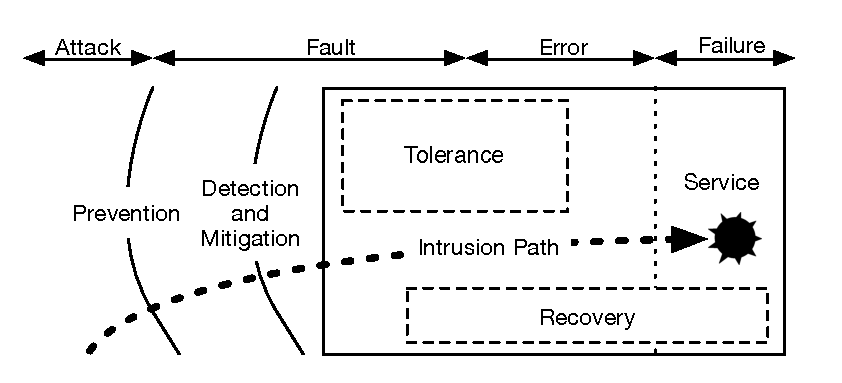
\includegraphics[width=110mm]{images/intrusion}
\caption{Intrusion path across the system}
\label{fig:intrusion_path}
\end{figure}

%prevention
\emph{Intrusion forecast and prevention} are realized by design and they seek to prevent future attackers from exploiting vulnerabilities. However, preventing intrusions by design is hard. Software has flaws due to its complexity and budget/time constraints \cite{Charette2005,Landwehr1992}. System administrators, as humans, can make security configuration mistakes or users may grant access to attackers \cite{Brown2001}. Moreover attackers can spend years developing new ingenious and unanticipated intrusions having access to what protects the system while the guardians have to predict them. Due to this asymmetry, it is arguably impossible to protect all vulnerabilities by design. Therefore the vulnerabilities of prevention mechanisms can be exploited successfully leading to an intrusion. A vast number of vulnerabilities and attacks are listed for instance in the National Vulnerability Database \cite{nistNVD}.\\

\emph{Intrusion detection and mitigation} mechanisms monitor the system to detect suspicious actions that may be connected with an intrusion. However, \acf{IDS} turn the system attack-aware but not attack-resilient, that is, they cannot maintain the integrity and availability of the system in face of attacks \cite{Ammann2002}. \acf{IDS} may not detect unknown vulnerabilities. Moreover, attackers may use encrypted actions or use legitimate requests.\\

%Intrusion Tolerance
\emph{Intrusion tolerance} is the last line of defense against attacks before the system failure occurs (Figure \ref{fig:intrusion_path}). Intrusion tolerance is the ability of a system to keep providing a, possibly degraded but adequate, service during and after an intrusion \cite{Stavridou2001a}. Instead of trying to prevent every single intrusion, these are allowed, but tolerated. The system has mechanisms to prevent the intrusion from generating a system failure \cite{Verissimo2003}. Intrusion tolerance mechanisms hide the errors effects using redundancy mechanisms or using intrusion recovery systems, which detect, process and recover from intrusions.\\

Many intrusion tolerance mechanisms are based on replicating state with Byzantine fault-tolerant protocols \cite{Schneider1990,Castro2002,Veronese2011}. The idea is to ensure that a service remains operational and correct as long as no more than a certain number of replicas are compromised. Replicas can be implemented in different manners to provide diversity, to reduce the risk of common failure modes. In addition, a proactive recovery mechanism can reboot the replicas periodically to rejuvenate and restore their soft-state and security assets, e.g., keys \cite{Candea2001,Castro2002,Sousa2010}. In \emph{disaster recovery} solutions, the state is replicated in remote sites, allowing the recovery from catastrophes that destroy a site \cite{cloud-disaster}.\\

The above-mentioned replication mechanisms for intrusion tolerance can tolerate some intrusions targeted at design faults (vulnerabilities), as long as diversity is used. However, most of the fault tolerance mechanisms do not prevent accidentally or malicious faults at application level, e.g., using valid user requests. Most of state replication mechanisms facilitate the damage to spread from one site to many sites as they copy data without distinguishing between legitimate and malicious sources. Furthermore, most of proactive recovery techniques rejuvenate only the application soft-state but intrusions can affect its persistent state. Consequently, intrusions may transverse these intrusion tolerance mechanisms and cause a system failure. 


\section{Intrusion Recovery}
\label{sec:related:recovery}
The main focuses of this thesis are intrusion recovery mechanisms that accept intrusions but detect, process and recover from their effects. These mechanisms remove all actions related to the intrusion, their effects on legitimate actions and return the application to a correct state. These mechanisms can be used to tolerate intrusions or to recover from system failures. In order to recover from intrusions and restore a consistent application behavior, the system administrator detects the intrusion, manages the exploited vulnerabilities and removes the intrusion effects. This process should change the application state to an intrusion-free state.\\

%Detection
The first phase of intrusion recovery, out of the scope of this work, concerns the intrusion detection. Automated \ac{IDS} are used to detect intrusions or suspicious behaviors. This phase may need human intervention to prevent false positives, which trigger recovery mechanisms and can result in legitimate data losses. Thus the detection phase can be a significant delay. The detection delay should be minimized because intrusion effects spread in the meantime between intrusion achievement and detection. Moreover, intrusion recovery services should provide tools to help system administrators to review the application behavior and determine which weaknesses were exploited. \\

%Correction: Vulnerability repair
The second phase, also out of the scope of this work, is vulnerability management. Vulnerabilities are identified, classified and mitigated after their detection by a group of persons which the \acf{NIST} names as the patch and vulnerability group \cite{Mell2005}. Vulnerabilities are fixed by configuration adjustments or applying a security software patch, i.e., by inserting a piece of code developed to address a specific problem in an existing piece of software. \\

%Eliminar os efeitos: dependence ficheiros afectados, etc
The third phase, and the one that this work is about, consists in removing the intrusion effects. Intrusions affect the application integrity, confidentiality and/or availability. To recover from availability or confidentiality violations is out of the scope of this document. However, we argue that the design of the applications should encompass cryptography techniques which may reduce data relevance and protect the data secrecy \cite{Maheshwari2000}.

Intrusion removal processes recover from integrity violations recreating an intrusion-free state. Due to the fact that the system availability is result of the integrity of each system component \cite{Wang2007}, these processes contribute to recover the system availability. Moreover, the removal processes should not reduce the system availability. We argue that intrusion recovery services should avoid the system downtime and support the execution of recovery processes in background without externalization to users. Intrusion recovery mechanisms can accomplish some of the goals of intrusion tolerance if they keep providing a, possibly degraded but adequate, service during and after an intrusion recovery.

The following sections explain distinct recover processes where the application integrity is restored by determining the effects of the detected intrusion actions, reverting them and recreating a correct state. 

\subsection{Formalization of the Recovery Process}
\label{sec:related:recovery_models}
As discussed in previous section, intrusion recovery services detect the intrusion effects, revert them and restore the application to a correct state. Here we explain this process by formally modeling the application as a sequence of actions and outline the distinct approaches to perform intrusion recovery. \\ 

An application execution is modeled as a set of actions $A$ and a set of objects $O$. Actions are described by a type (read, write, others more complex), the value(s) read/written, and a timestamp (which defines the order of the actions). Each object has a state or value and a set of operations that can modify it. We specify $A_{intrusion}$ as the subsequence of actions of $A$ whereby the attacker compromises the application during the intrusion, $A_{after}$ as the subsequence of actions that begins after the intrusion begin (including the first action of the intrusion) and $A_{legal}$ as the subsequence of legitimate actions in $A$. Notice that $A_{legal} = A - A_{intrusion}$. 

A recovery service aims to set the state of a service to $O_{recovered}$ at the end of the recovery process. The set $O_{recovered}$ shall be composed of objects as if their state was defined exclusively by a set of legitimate actions $A_{recovered}$. Objects of the subset $O_{recovered}$ represent a new \textit{intrusion-free} and \textit{consistent state}. A state is consistent if it is valid according to the application specification. A state is intrusion-free if it is created only by legitimate actions. If the application respects the specification (correctness), then changing from $O$ to $O_{recovered}$ performs service restoration \cite{Aviz}, i.e., restores the application service to a correct behavior.

A basic recovery service, like a full-backup mechanism, tries to obtain, after the recovery, the subset of object values $O_{recovered}$ written before the intrusion, which do not include the attacker actions, i.e., $O_{recovered} = D - D_{after} : D_{recovered} \cap D_{intrusion} = \emptyset$.

We define the set of \textit{tainted} actions, $A_{tainted}$, and the set of tainted objects, $O_{tainted}$, at a certain instant in the following way: if an action belongs to $A_{intrusion}$, then it belows to $A_{tainted}$; if an object belongs to $O_{intrusion}$ then it belongs to $O_{tainted}$; if an action in $A_{legal}$ reads an object in $O_{tainted}$, then that action belongs to $A_{tainted}$; if an action in $A_{tainted}$ writes an object value in $O_{legal}$, then that object belongs to $O_{tainted}$ (Figure \ref{img:sets}). Therefore, $A_{tainted}$ includes $A_{intrusion}$ but typically also actions from $A_{legal}$ that were corrupted by corrupted state. Also, $O_{tainted}$ includes $O_{intrusion}$ but typically also objects from $O_{legal}$ that were corrupted by corrupted state. Then, the set of object values written only by non-malicious actions is not the same as the set of objects obtained after removing the objects written by malicious or tainted actions, i.e., $O_{legal}$ written by $A \cap A_{intrusion} = \emptyset$ is not equal to $O_{legal}$ written by $D-D_{intrusion}$ or $O_{legal}$ written by $D-D_{tainted}$. In other words, to remove the objects written by intrusions and tainted actions is necessary but not enough to obtain the values of the set of objects that would be produced only by legitimate actions.

Some intrusion recovery systems \cite{taser,itdb,phoenix} attempt to obtain $O_{recovered}$ where the values of the objects of $O_{tainted}$ are removed from the current state $O$. To do so, the value of each object in $O_{tainted}$ is replaced by a previous value. These systems keep the objects written by legitimate actions, $O_{legal}$, unmodified. \\


\begin{figure}
  \centering
  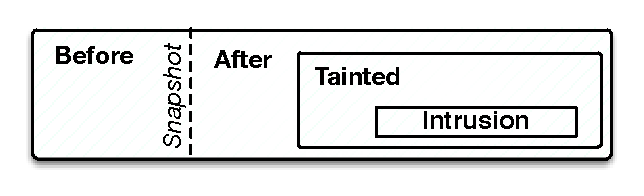
\includegraphics[width=80mm]{images/sets}
  \caption{Set of actions of an application execution}
  \label{img:sets}
\end{figure}


Consider an hypothetical application execution at a certain point in time, after the intrusion, where $A$ is replaced by the set $A_{recovered} = A - A_{intrusion} = A_{legal}$, i.e., where the intrusion actions $A_{intrusion}$ are not executed. We would have in this application: $A \cap A_{intrusion} = \emptyset \implies D_{intrusion} = \emptyset, A_{tainted} = \emptyset \implies D_{tainted} = \emptyset$. In other words, if the malicious actions are removed, then the state $O$ does not have the objects written by $A_{intrusion}$. For this reason, the sequence of tainted actions $A_{tainted}$ is empty. The set of tainted actions in the real application execution, which includes $A_{intrusion}$, would read different values and have a different execution if $A_{intrusion}$ would be empty. Therefore, if $A_{intrusion}$ and $O_{intrusion}$ are removed, then $A_{tainted}$ should be \emph{replayed} because the actions of $A_{tainted}$ are not contaminated by malicious data during their re-execution. The replay process restores the application to a correct state $O_{recovered}$, which is intrusion-free.\\

The sequence of actions, $A_{before}$, performed before the intrusion, i.e., $A_{before} = A - A_{after}$, can be extensive. Each action takes a variable but not null time to perform. Therefore, to replay $A_{recovered} : A_{before} \subseteq A_{recovered} $ may takes an excessive amount of time. We define the subsets $O_{snapshot}(t)$ and $A_{snapshot}(t) : A_{snapshot} \subseteq A$ as the subsets of object values and actions executed before the begin of a snapshot operation at instant \textit{t}. The snapshot operation copies the value of the object immediately or on the next write operation. If the attack is subsequent to $t$, then $A_{after} \cap A_{snapshot} = \emptyset \implies (A_{intrusion} \cup A_{tainted}) \cap A_{snapshot}(t) = \emptyset$, i.e., the snapshot is not affected by intrusion. For that reason, the service can replay only $A-A_{snapshot}-A_{intrusion}$ using the object set $O_{snapshot}$ as base. 


The most recent works, which are explained in the following sections, define two distinct approaches to update the set of object $O$ to $O_{recovered}$ because of changes in the execution of $A_{tainted}$: \textit{rewind} and \textit{selective replay}. The selective replay approach loads only the previous versions of the tainted objects, $O_{tainted}$, and replays only the legitimate operations, which were tainted, $A_{tainted} \notin A_{intrusion}$, to update the objects in $O$. The $O_{legal} \notin D_{tainted}$ remain untouched. The alternative approach, rewind \cite{Brownc}, designates a process that loads a system wide snapshot previous to the intrusion moment and replays every action in $A-A_{snapshot}-A_{intrusion}$. However, this process can take a long time. \\


A \textit{version} is a snapshot of a single object value before the instant $t$. They can be recorded with the sequence of actions that read or write them before the instant $t$. We define a \textit{compensating} action as an action that reverts the effects of an original action, for instance writing a previous value. A compensation process can obtain a previous snapshot or version. For this propose, we define the sequence $A_{compensation}(t)$ as the compensation of $A_{posteriori}(t)$, the sequence of actions after instant $t$. The compensation process applies the sequence of compensating actions $A_{compensation}(t)$ on the current version of the objects, in reverse order, to obtain a previous snapshot or version.\\

Recovery services have two distinct phases: \textit{record phase} and \textit{recovery phase}. The record phase is the service usual state where the application is running and the service records the application actions. In order to perform replay, the application actions do not need to be idempotent but their re-execution must be deterministic. The record phase should record the actions input and the value of every non-deterministic behavior to turn their re-execution into a deterministic process. The recovery phase can have three phases: determine the affected actions and/or objects, remove these effects and replay the necessary actions to recover a consistent state, as already explained in Section \ref{sec:related:recovery}. The recovery services that support \textit{runtime recovery} do not require application downtime because the record and recovery phases can occur simultaneously.\\


Most of intrusion recovery services record the actions and track the objects accessed by each of them. Since the actions read and write objects from a shared set of object values $O$, we can establish dependencies between actions. Dependencies can be visualized as an \textit{action dependency graph} or an \textit{object dependency graph}. Nodes of an action dependency graph represent actions and the edges indicate dependencies though shared objects. The object dependency graph establishes dependencies between objects through actions. Dependency graphs are used to order the re-execution of actions \cite{undoForOperators}, get the sequence of actions affected by an object value change \cite{warp}, get the sequence of actions tainted by an intrusion \cite{goel} or resolve the set of objects and actions that caused the intrusion using a set of known tainted objects \cite{backtracker}. 

A \textit{taint algorithm} aims to define the tainted objects $O_{tainted}$ from a source sequence of malicious actions $A_{intrusion}$ or objects $O_{intrusion}$ using the dependency graph. The \textit{taint propagation via replay} \cite{retro} algorithm begins with the set of $O_{intrusion}$ determined by the base taint algorithm and expands the set $O_{tainted}$. It restores the values of $O_{intrusion} \cup D_{tainted}$ and replays only the legal actions that output $O_{intrusion} \cup D_{tainted}$ during the first execution. Then it replays the actions dependent from $O_{intrusion} \cup D_{tainted}$, updating their output objects. While the forward actions have different input, they are also replayed and their outputs are updated.\\

Dependencies are established during the record phase or at recovery time using object and action records. The level of abstraction influences the record technique and the dependency extraction method. The abstraction level outlines the recoverable attacks. In the next paragraphs, we explain the relevant works at abstraction levels where services deployed in \ac{PaaS} are attacked: operating system, database and application.\\


\subsection{Recovery at Operating System Level}
\label{sec:related:recovery_os}

In this section, we present the main intrusion recovery proposals for operating systems. First, we present the proposal that introduced the main dependencies for operating systems. Then, we present two intrusion recovery systems that use dependency rules and tainting propagation via replay, respectively. Finally, we present proposals to recover from intrusions in computing clusters, virtual machines and network file systems.\\

\textbf{BackTracker \cite{backtracker}:} Backtracker proposes a tainting algorithm to track intrusions. It does not perform any proactive task to remove or recover from intrusions but provides a set of rules for intrusion recovery in operating systems.

Backtracker proposes a tainting algorithm that does tainting analysis offline, after attack detection, as follows. First a graph is initialized with an initial set of compromised processes or files, $O_{tainted}$, identified by the system administrator. Then, Backtracker reads the log of system calls from the most recent entry until the intrusion moment. For each process, if it depends on a file or process currently present in the graph then the remaining objects dependent from the process are also added to the graph. The result is a dependency graph (Figure \ref{fig:backtracker_graph}) with the objects, including $O_{intrusion}$, which the compromised objects depend on. The following dependency rules establish the graph edges:

\begin{itemize}
\item \textit{Dependencies process-process:}
\begin{itemize}
\item \textit{Process depends on its parent process}: Processes forked from tainted parents are tainted.
\item \textit{Thread depends on other threads}: Clone system calls to create new threads establish bi-directional dependences since threads share the same address space. Algorithms to taint memory addresses \cite{bezoar} have a significant overhead. Signaling communication between processes also establish dependencies.
\end{itemize}
\item \textit{Dependencies process-file:}
\begin{itemize}
\item \textit{File depends on Process:} If the process writes the file.
\item \textit{Process depends on File:} If the process reads the file. 
\end{itemize}

\item \textit{Dependencies process-filename:}
\begin{itemize}
\item \textit{Process depends on filename:} If the process issues any system call that includes the filename, e.g., open, create, link, mkdir, rename, stat, chmod. The process is also dependent of all parent directories of file.
\item \textit{Filename depends on process:} If any system call modifies the filename, e.g., create, link, unlink, rename.
\item \textit{Process depends on directory:} If the process reads one directory then it depends on every all filenames on directory.
\end{itemize}
\end{itemize}

\begin{figure}
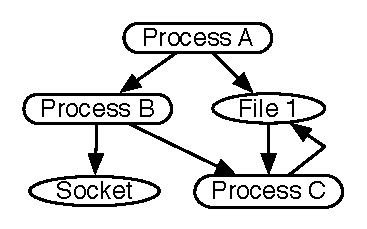
\includegraphics[height=30mm]{images/depGraph}
\centering
\caption{Dependency graph generated by BackTracker}
\label{fig:backtracker_graph}
\end{figure}

Objects shared between many processes, e.g., \textit{/tmp/} or \textit{/var/run/utmp} are likely to produce false dependencies leading to false positives. Therefore, Backtracker proposes a \textit{white-list} filter that ignores common shared files. However, this technique relies in the system administrator knowledge. Moreover, it generates false negatives because it allows the attackers to hide their actions in objects that belong to the white-list. \\


\textbf{Taser \cite{taser}:} Taser removes the intrusion effects from the file system used by the operating system. To do that, it loads a previous version of each tainted file, $O_{tainted}$, from a file-system snapshot, $O_{snapshot}(t)$. Then, to recover the tainted objects, it replays the legitimate modification actions of each tainted object since the snapshot instant $t$.

%record phase
Taser relies on Forensix \cite{forensix} to audit the system actions during the record phase. Forensix logs the names and arguments of every system call related to process management, file system operations and networking. In order to determine the intrusion effects, Taser builds a \textit{object dependency graph} using a set of rules similar to the rules of Backtracker \cite{backtracker}. The object definition encompasses files, sockets and processes. Since these rules result in a large number of false dependencies, which mark legitimate objects as \textit{tainted}, Taser provides not only a white list mechanism but also establishes optimistic policies that ignore some dependencies. However, attackers can leverage these optimistic policies to penetrate the operating system.

%How it determines the affected elements?
The recovery phase is started with a set of tainted objects provided by an system administrator or an \ac{IDS}. The provided set of objects can either be the source or the result of an attack. In the latter case, Taser, like Backtracker \cite{backtracker}, transverses the dependency graph in reverse causality order to identify the set of attack source objects, $O_{intrusion}$, which compromised the provided objects. After, at \textit{propagation phase}, Taser transverses the dependency graph from the source objects of the attack, $O_{intrusion}$, to the current moment, adding all tainted objects to the set $O_{tainted}$.

%how it removes
Taser removes the intrusion effects loading a previous version of the tainted objects from a file-system snapshot, $O_{snapshot}(t)$. Then, to recover a coherent state, Taser performs \textit{selective replay}, i.e., it replays, sequentially, the legitimate write operations of the tainted files since the snapshot. Non-tainted files remain unchanged. Since Taser does not checkpoint the state of processes nether the input of each system call, the system must be restarted to remove the current non-persistent states and processes must be replayed from the beginning to load their non-persistent state and perform their system calls with the correct state. This issue has a significant overhead specially for long-run processes as web servers.


%does it replays? analyze
Taser does not update the objects originally dependent from tainted objects. In other words, the replay process only recovers a consistent state for the originally tainted objects. Therefore, Taser ignores the set of actions that read the modified version of the tainted files and have a different execution and output. This problem is addressed in \cite{Shafique2006}. Moreover, Taser uses rules to determine the affected files and remove their effects, so it can mistakenly mark legitimate operations as tainted and induce to legitimate data losses.\\



\textbf{RETRO \cite{retro}:} RETRO provides the capability of removing files affected by a set of identified attacking actions. It restores the corrupted files to a previously version using a file system snapshot and then performs selective replay using \textit{taint propagation via replay}. 

%Record Phase:
During the record phase, the kernel module of RETRO creates periodic snapshots of the file system. RETRO logs the input and the output objects of each system call and their associated process. The object definition encompasses not only files and directories but also \ac{TCP} sessions and the operating system console (tty). Dependencies are established per system call instead of per process. Therefore, the graph is finer-grained than the graph of Backtracker \cite{backtracker} and reduces the number of false positives.

%remove
During the recovery phase, RETRO requires the system administrator to identify $A_{intrusion}$, processes, system calls or $O_{intrusion}$ objects which caused the intrusion. First, it removes the malicious system calls from the graph. Then it performs \textit{taint propagation via replay}. To do so, it loads a previous version, from a snapshot, of the objects in $O_{intrusion}$. Then, the system calls, which are dependent from the restored objects, are replayed and their output objects are updated. The forward system calls, which depend on the updated objects, are also replayed while their inputs are different from the first execution. The propagation is done thought the output of system calls with different execution. The recovery process terminates when propagation stops. Since RETRO records the system call input, it can replay processes with system call granularity instead of process granularity, so the replay process may stop earlier. However, this mechanisms forces that the process re-execution has the same sequence of system calls as its first execution. Therefore, the process source code nether its sequence of actions can not change. 

%external dependencies
Since RETRO replays the processes, the external state may change. External changes are manifested through operating system console and network objects. RETRO emails the system administrator with the textual difference between the original and recovery outputs. Later work of the same authors, \textit{Dare} \cite{dare}, extends RETRO to recover from intrusions in distributed systems. It adds the dependencies through sockets. Machines involved in a network session add socket objects to the dependency graph. Network protocol, source and destination \ac{IP} and ports and one ID, which are exchanged in every package during the connection, globally identify each socket object. The recovery phase in Dare is similar RETRO except on network system calls handlers. Compromised network sessions must be replayed since their input depends on destination server. Therefore, prior to invoke the system call for network session establishment, Dare invokes a remote method at receiver Dare daemon to rollback the network session. The receiver rollback the dependent objects to the version before session establishment and replays their dependencies. The remote method response includes the re-execution output. The local system updates the system call output. The re-execution is propagated if this output is different. 

%Analyse
The efficiency of RETRO comes from avoiding to replay the actions if their input remains equal. However, the invoked system call must remain the same. Therefore, RETRO does not support a distinct process execution. RETRO requires human intervention to solve external inconsistencies. Dare solves it but it is limited to clusters where every operating system runs a Dare and RETRO daemon. RETRO can not recover from an intrusion whose log files have been garbage collected or deleted. Dare supports distributed re-execution but, as RETRO, the affected machines must be offline because its propagation algorithm shutdown the service during the repair phase. \\



\textbf{Bezoar \cite{bezoar}:} Bezoar proposes a rewind based approach to recover from attacks coming from the network in virtual machines (VM). The snapshot is performed by \ac{VM} forking using copy-on-write. This snapshot technique encompasses the entire system: processes and kernel spaces, resources, file system, virtual memory, \ac{CPU} registers, virtual hard disk and memory of all virtual external devices. Bezoar tracks how the data from network connections propagates in memory. During the recovery phase, the system administrator identifies the network connections used by the attackers. Bezoar removes the intrusion effects using rewind. It loads a previous \ac{VM} snapshot and it replays the system execution ignoring all network packets from the identified malicious sources. 

The recovery process using rewind is longer than RETRO or Taser because all external requests are replayed but supports distinct process execution. Bezoar requires system outage during the replay phase and does not provide any external consistency warranties.\\


\textbf{Repairable File System (RFS) \cite{rfs}:} RFS is designed to recover compromised network file systems. The novelty in RFS comparing with the previously introduced systems is its client-server architecture. RFS includes a client and a server module for a network file system (NFS).

The client module tracks the system calls using ExecRecorder \cite{Oliveira2006} and establishes the dependence between processes and NFS requests. Every request to the NFS server is marked with a request ID and the client ID. At server side, the request interceptor logs all requests sent by clients to update files. Requests are ordered in per-filename queues. They are processed locally and write operations are mirrored to external server asynchronously after reply. The external server keeps all file versions. 

During the recovery phase, the server defines the contaminated processes using the client logs. A process is contaminated if it matches a set of rules similar to Backtracker \cite{backtracker}. RFS adds the concept of contaminated file and contaminated file block. If a file is contaminated, all its blocks are contaminated. The reverse is not true, i.e., processes remain non-contaminated if they read a legitimate block of a contaminated file. RFS uses the version server to rollback only the affected files. \\



\textbf{Summary:} Dependencies at the operating system level are established by rules based on BackTracker \cite{backtracker}. These rules are vulnerable to false positives and false negatives. While Taser \cite{taser} and RFS \cite{rfs} recover from intrusions removing the effects only in corrupted files, RETRO \cite{retro} removes the values written by $A_{intrusion}$ and replays the forward system calls while their input changes. If $A_{intrusion}$ is identified properly, then RETRO does not have false positives.

The operating system level services are vulnerable to attacks inside kernel because they only audit the system calls. Attackers can compromise the recovery system because the log daemons are installed in the machine where attacks are performed. The recovery guarantees are limited by the system administrator capability to detect the attack and pinpoint the intrusion source. System administrators must avoid false positives to prevent legitimate data losses. However, remove false dependencies can take a while because the low abstraction level creates bigger dependency graphs and logs.




\subsection{Recovery at Database Level}
\label{sec:related:recovery_database}

A vast number of database management systems (DBMS) support recovery by loading a snapshot (or full-backup) of the database, possibly patched with blocks of data modified since the snapshot was taken. However, this approach does not distinguish between malicious and legitimate requests. The recovery approach we are interested in the document is applied to databases similarly to what was seen in Section \ref{sec:related:recovery_os} for operating systems. While the operating system dependencies are established by the system calls, the database dependencies are established by transactions. First, we define the main dependencies in the database systems. These rules are used by most of the recovery services for databases and applications (Section \ref{sec:related:recovery_app}).\\

Compromised transactions are determined from an initial set of bad transactions using read and write rules. ``Transaction $ T_j$ is dependent upon transaction $ T_i$ if there is a data item $x$ such that $T_j$ reads $x$" \cite{Ammann2002} and $T_i$ performs the latest update on $x$. Transaction dependency is transitive. ``A good transaction $G_i$ is suspected if some bad transaction $B_i$ affects $G_i$. A data item $x$ is compromised if $x$ is written by any bad or suspect transaction" \cite{Ammann2002}. This dependency chain is broken if a transaction performs a blind write, i.e., the transaction writes an item without read it first.

However, legitimate transactions can have different outputs even when their first execution were not tainted. For example, a malicious transaction can remove a data item which the following transactions would read and then write other data items. Since user mistakes are often deletes due to wrong query arguments, this is a relevant issue. Xie \textit{et al.} \cite{Xie2008} propose to track the transaction that deleted the data items keeping a copy of deleted data items in a separated database table. To add the dependencies from the deleted data items, the \ac{SQL} statement is performed in the original and delete tracking tables. 

The dependency rules require to extract the read and the write set of each transaction, i.e., the set of data items that each transaction read or modifies. The following proposals use different methods to extract these sets and restore the tainted data items.\\


\textbf{ITDB \cite{itdb,Ammann2002,Wang2007}:} Intrusion Tolerant Database (ITDB) performs intrusion recovery in databases using compensating and supports \textit{runtime recovery}, i.e., the database service remains available during the recovery process. ITDB uses the generic set of dependency rules mentioned in the beginning of Section \ref{sec:related:recovery_database} and extracts the read and write set parsing the \ac{SQL} statements.

During the record phase, ITDB audits the read and write sets of each transaction. Most relational \ac{DBMS} only keep write logs. Therefore, Liu \textit{et al}. \cite{itdb} propose a pre-defined per-transaction type template to extract the read set of parsed \ac{SQL} statements. This approach is application dependent since updates in application queries require updates in their templates. 

%algoritmo de recovery
At recovery phase, ITDB initiates a set $O_{tainted}$ with the intrusion source data items. Then, it reads the logged read and write sets of each transaction from the intrusion moment to the present. For each transactions, ITDB keeps the write set until the transaction commits or aborts; if the transaction commits after reading some data item that belongs to $O_{tainted}$, ITDB adds the data items in the transaction write set to $O_{tainted}$ and the transaction must be compensated. The compensating of a transaction reverts the effects of the original transaction. It performs the inverse modification of the original transaction to restore the previous values. Repaired entries in $O_{tainted}$ are tracked to prevent compensating of later transactions from restore a repaired data item to its version after the attack. After this process, the latest legitimate value of $O_{tainted}$ entries is recovered.

%extras
If the intrusion propagation is faster than the recovery process then the recovery phase is endless because the damage will spread through new transactions. To prevent damage spreading, ITDB blocks the read accesses to the data items in $O_{tainted}$. Since identification of $O_{tainted}$ requires log analysis, Liu \textit{et al.} propose a \textit{multi-phase damage container} technique to avoid damage spread through new requests during the recovery phase. This damage containing approach denies the read access to the data items were written after the intrusion. Then, during the recovery phase, it releases the data items that were mistakenly contained. This approach speeds-up the recovery phase and confines the damaged data items. Moreover, it supports \emph{runtime recovery}. However it decreases the system availability during the recovery period and degrades the performance.

An alternative approach concerns the throughput asymmetry between the recovery and the user flows. The asymmetry can be neutralized if the repair request priority is increased. Then, the availability is not compromised anymore but users may read tainted data and propagate the damage slower. 

The ITDB architecture includes an \acf{IDS}. The \ac{IDS} is application aware and acts at transaction level. Liu \textit{et al.} propose isolation in terms of users: when a suspicious transaction is reported by the \ac{IDS}, every write operation from the suspicious user is done in isolated tables.

The ITDB does not perform transaction replay during the recovery phase. Therefore, it ignores that legitimate executions can be influenced by the updated values. Liu \textit{et al.} propose a theoretical model \cite{Yu2003} based on possible workflows and versioning. However, predict every possible workflow requires extensive computational and storage resources. \\


\textbf{Phoenix \cite{phoenix}:} Phoenix removes the intrusion effects using a versioned database. While Liu \textit{et al.} \cite{Ammann2002} rely on templates of \ac{SQL} statements and read the log in recovery time, Phoenix changes the \ac{DBMS} code to extract read dependencies and proposes a runtime algorithm to check dependencies between transactions.

%Versioning
Phoenix performs every write operation appending a new row to the table. This new row includes an unique transaction id to support the restoration of previous row versions. Phoenix modifies the PostgreSQL \ac{DBMS} code to intercept read queries during their execution and to extract the transaction id of each accessed row. The logged data is used to update the dependency graph.

%Como funciona
At the recovery process, Phoenix identifies the set of affected transactions, $A_{tainted}$, from a root set of malicious transactions, $A_{intrusion}$, using the dependency graph. Then, it changes these transactions status to \textit{abort} in the PostgreSQL transaction log. Since PostgreSQL, in serializable snapshot isolation mode, exposes only the row version of the latest non-aborted transaction, the row is restored and the effect of tainted transactions are removed.\\


\textbf{Summary:} Recovery systems for relational databases differ on their methods to track the read and write sets and to restore previous values. ITDB is application dependent because it requires pre-defined templates to parse the \ac{SQL} statements. On the other hand, Phoenix is application independent but \ac{DBMS} dependent because it modifies the \ac{DBMS} source code and relies on the usage of serializable snapshot isolation mode. 

ITDB is records the previous versions in contrast to Phoenix which just records the transactions. The first requires more storage capacity to save versions, the second requires the knowledge of the compensating of each transaction and more computation resources during recovery to revert the tainted transactions.

The data item granularity affects the runtime performance overhead and the accuracy of dependency tracking. Coarser granularity, e.g., row, results in lower performance overhead but a higher probability of false dependence if two transactions read and write different portions of the same data item. Moreover, an attack can compromise just an independent part of the transaction and legitimate data is removed. 




\subsection{Recovery at Application Level}
\label{sec:related:recovery_app}

Web applications are the main type of application which is deployed in \ac{PaaS}. These applications are usually composed of a three tier architecture: presentation tier, application-logic tier and data tier. The following works assume the data tier to be a database. 
Previous section works establish the dependencies between transactions using their read and write sets. However, they ignore the dependencies between transactions at application level. For example, an application can read a record A through a transaction 1, compute a new value B, based on A, and write the value B through a transaction 2. The application-logic tier is often state-less, the requests are independent and the database is the only mean of communication between requests (Section \ref{sec:arch:paas}).\\ 


\textbf{Data Recovery for Web Applications \cite{goel}:} Goel \textit{et al.} propose a recovery service that selectively removes intrusion effects from web applications that store their persistent data in a \ac{SQL} database. Since each user request may involve multiple transactions, it tracks the user, the session, the request and the accessed rows. The proposal uses a tainting algorithm and compensating transactions.

During the record phase, a monitor logs each user request and the database rows and tables read and written by the transactions associated with it. Transactions are stamped with an id that establishes the replay order, since the database uses serializable snapshot isolation.

The recovery phase is as follows. First, the system administrator, using the logged data, identifies the malicious requests $A_{intrusion}$. Then, using a dependency graph, it determines the tainted requests. The dependency between transactions is established in a similar manner to the Section \ref{sec:related:recovery_database} but using table granularity instead of row granularity. Such coarse-grained approach may generate many false dependencies. Therefore Goel \textit{et al.} use \textit{taint propagation via replay}. Moreover, it proposes to modify the PHP-interpreter to reduce the false dependencies between transactions using a variable-level tainting. In other words, variables that read tainted rows or fields are also tainted; rows or fields written by tainted variables are tainted. This process increases the precision of the set of tainted requests. Finally, the compensation transactions of the tainted requests are applied in reverse serialization order on the current state of the database to selectively revert the effects of the database operation issued by the tainted requests.\\ 

\textbf{POIROT \cite{poirot}:} POIROT is a service that, given a patch for a newly discovered security vulnerability in a web application code, helps system administrators to detect past intrusion that exploited the vulnerability. POIROT does not recover from intrusions but proposes a tainting algorithm for application code. During the normal execution, every user request and response is stored. The log of each request includes the invoked code blocks. After the attack discover phase, the software is updated to fix its flaws. POIROT identifies the changed code blocks and requests dependent from them during the normal execution. The affected requests are replayed. During the re-execution phase, each function invocation is forked into two threads: the updated e non-updated version \cite{Wang2011}. Functions invocations are executed in parallel and their output are compared. If outputs are similar, only one execution proceeds otherwise the request execution stops since the request was affected by code patch. These concepts are used in Warp \cite{warp}.\\


\textbf{Warp \cite{warp}:} Warp is a patch based intrusion recovery service for single server web applications backed by a relational database. Unlike previous approaches, Warp allows system administrators to retroactively apply security updates without tracking down the source of intrusion and supports attacks at user browser level. Warp is based on RETRO \cite{retro} \emph{taint propagation via replay} approach and removes the intrusion effects using a versioned database. The Warp prototype uses PHP and PostgreSQL. 

%normal
During the normal execution, Warp uses a client browser extension to record all JavaScript events that occur during the visit of each page. For each event, Warp records the event parameters, including the target \acf{DOM} element. \ac{HTTP} requests are stamped with a client ID and a visit ID to track dependencies between requests at browser level. On server side, Warp records every requests received and forwards the request to the PHP application. Since Warp uses PHP, an interpreted language, it records which files were used during the original request execution and records the non-deterministic functions. Warp stores the database queries input/output and tracks the accessed table partitions using a \ac{SQL} statement parser. To conclude, the \ac{HTTP} response is logged and packed with all execution records.

Warp includes a time-travel versioned relational database. Each row is identified using a row ID and includes a \textit{start time} and \textit{end time} timestamp columns that establish the row validity period. Warp reverts the intrusion effects, in a specific row, loading one of its previous versions. Warp supports concurrent repair using more two integer columns to define the begin and end of each \textit{repair generation}. At repair phase, the current repair generation ID is incremented to fork the database. User requests are performed in the current generation while recovery requests are perform in the next generation. After replaying the requests retrieved until the beginning of the repairing process, the server stops and applies the remain requests.

%Como determina
During the repair phase, the system administrator updates the application software to fix its flaws. Then, Warp determines the requests used the modified source code files \cite{poirot,Wang2011}. These requests are the root cause of changes during the re-execution. To update the database and reflect the patch, each user request is replay using a server-side browser and taint propagation via replay. The modified PHP interpreter intercepts non-deterministic function calls during the replay and returns the original logged value. Also, database read queries are replayed only if the set of affected rows is different or its content was modified. Write queries are replayed loading a previous version of the rows and replaying the \ac{SQL} statement. Each row, which has a different result after re-execution, is now tainted and all requests that read the row are also marked to replay in the browser. Finally, the \ac{HTTP} response is compared with original. If responses are different, the following dependent user interactions are replayed in the server side browser.

%Extra
The server-side browser may fail to replay the original user request. The request may depend on a reverted action of the attacker. These conflict cases are queued and handled by users later. 

%Comments 
Warp rewrites the \ac{SQL} statements, which are used by the application to perform write operations in the database, adding four extra columns per table: start/end timestamp and start/end generation. However, these columns may be a considerable storage overhead. It also depends on a client browser extension to log and modify every request. Warp is designed for single machine applications: it does not support application deployed in multiple servers or distributed databases since versions are timestamp based. \\


\textbf{Aire \cite{aire}:} Aire is an intrusion recovery service for loosely coupled web services. It extends the concept of local recovery in Warp \cite{warp} tracking attacks across services. While Dare \cite{dare} aims to recover a server cluster synchronously using RETRO \cite{retro} in each node operating system, Aire performs recovery in asynchronous third-party services using Warp \cite{warp}. 

Aire prevents the recovery process from locking due to remote servers downtime. To achieve this goal, the pendent repair requests are queued until the remote server is recovered. Since clients may see a partial repaired state, Aire proposes a model based on eventual consistency \cite{Decandia2007,Vogels2009}. The model allows clients to observe the result of update operations in different orders or delayed during a period called \textit{inconsistency window}, i.e., until the remote server recovers. Aire considers the repair process as a concurrent client. To repair key-value database entries, Aire creates a new branch \cite{git} and re-applies legitimate changes. At end of local repair, Aire moves the current branch pointer to the repaired branch.

Like Warp \cite{warp}, during the normal execution, Aire records the service requests, responses and database accesses. Requests and responses exchanged between web-services, which support Aire, are identified using an unique ID to establish the dependencies.


The recovery phase is as follows. First, the system administrator identifies the corrupted requests. The system administrator can create, delete or replace a previous request or change a response to remove the intrusion actions. Second, Aire creates a new branch, which will contain the set of changes. Third, Aire does a local repair of the application in a similar manner to Warp \cite{warp}. In contrast to Warp \cite{warp}, starts the recovery process in remote servers if at least one of the requests or responses sent previously is modified. To do so, Aire sends a request to the source or destination of the modified message. If the remote server is offline, the repair requests are queued to be sent later. As repair messages propagate between the servers to start successive repairing actions, the global state of the system is repaired. However, clients may see an inconsistent state during this process. Therefore, Aire applications must support eventual consistency.  

The Aire approach using eventual consistency requires the developer to concern the conflict resolution. Moreover, Aire recovers third-party web-services, which must have an Aire daemon. Aire requires the system administrator to pinpoint the corrupted requests. Finally, Aire, as Dare \cite{dare}, requires application downtime during the recovery process.\\



\textbf{Undo for Operators \cite{undoForOperators}: }Undo for Operators allows the system administrators to recover from their mistakes, software problems or data corruption in email services with file system storage. The design is base on ``Three R's: Rewind, Repair and Replay" \cite{Brownc} where operator loads a system-wide snapshot previous to the intrusion, repairs the software flaws and replays the user-level requests to recover a correct application state. In contrast to the selective replay approach, where only the tainted entries are reverted, the rewind approach reverts all database entries. On one hand, this approach requires to replay more requests. On the other hand, the approach does not require to determine which data items are tainted because every entry is reverted.

Undo for Operators proposes a proxy interposed between the application and its users. The proxy intercepts application requests. Since requests most be ordered to replay, Undo for Operators defines the concept of \textit{verb}. Each protocol operation has its own \textit{verb} class. A verb object encapsulates a single interaction (request/response) of the user and exposes an interface to establish the order between requests and their dependencies. However, the proposed architecture is protocol dependent. The proxy implementation only supports \ac{IMAP} and {SMTP}. A new protocol requires a new set of verbs. 

During the normal execution, user requests are encapsulated into verbs and sent to a remote machine: the \emph{undo manager}. The undo manager uses the interface of verbs to define its dependency, i.e., if it can be executed in parallel or must have a causal order with other request. The dependency is established per verb type depending from the operation and its arguments. Thus, the dependency mechanism is application dependent. For example, send email operations (SMTP protocol) are commutable and independent because the email delivery does not have ordering guaranties. On the other hand, the order of delete (expunge) and list (fetch) operations in the same folder is relevant and they are not independent. If two verbs are dependent, the second is delayed upon the first is processed. This method establishes a serialization ordering but it can create a significant performance overhead on concurrently arriving interactions and requires protocol knowledge.

The recovery phase strategy is as follows. First the operator determines the corrupted verbs and fixes their order adding, deleting or changing verbs. Second, the application is \textit{rewind}, i.e., a system-wide snapshot is loaded to remove any corrupted data. Third, the operator patch the software flaws of the application. Finally, all legitimate requests started after the intrusion, $A_{legitimate}$, are re-sent by the proxy to rebuild the application state. 

External inconsistencies may come out when the requests are replayed. These inconsistencies are detected comparing the re-execution and the original responses. Different responses trigger a compensating action defined per verb to keep an external consistent state. Again, these actions are application dependent.

During the recovery process, Undo for Operators replaces the current system state by a system wide snapshot. Consequently, it does not support runtime recovery. Moreover, it relies on protocol knowledge to establish dependencies, compensating actions and to sort the requests during the normal execution and recovery phase. Therefore, any protocol change requires modifying the supported verbs. Intrusions can use corrupted requests which are not defined as verb classes and cause a system fail.\\


\textbf{Summary:} Goel \textit{et al.} and Warp \cite{warp} establish dependencies using the request read/write set of the database and use taint via replay. Undo for Operators \cite{undoForOperators} establishes dependencies using the knowledge of the operations protocol. Unlike Goel \textit{et al.}, Warp \cite{warp} and Undo for Operators \cite{undoForOperators} support application repair. Warp tracks the requests affected by the modified file. Undo for Operators replays every request using its proxy. While Goel \textit{et al.} ignores external consistence, Warp \cite{warp} detects inconsistencies in responses and replays the user interaction in a browser and Undo for Operators uses compensating actions based on protocol-specific knowledge.

Their approaches to remove the intrusion effects are also distinct. Goel \textit{et al.} uses compensating transactions to create a system wide snapshot, Undo for Operators loads a previous snapshot and Warp keeps the versions of each data item. If the tainted request are few, then Goel \textit{et al.} and Warp have a significant advantage because they replay only the tainted requests. On the other hand, Undo for Operators requires less storage than the remaining options. Moreover, the knowledge of inverse transaction is required to create the compensation of transactions. \\







\section{Chapter Summary}
\label{sec:related:discuss}
Previous subsections describe various services that use different approaches to recover from intrusions. The level of abstraction outlines the recorded elements. Intrusion recovery services at the operating system level record the system calls and the file system. At the database level they track the transactions. At the application level they track the transactions, requests and code execution (Table \ref{tab:storingTracking}). The log at operating system level is more detailed but may obfuscate the attack in false positive prevention techniques. At database and application level, the log is semantically rich but does not track low level intrusions.\\


Most of services require the system administrator to identify the initial set of corrupted actions or objects (Table \ref{tab:storingTracking}). The system administrator may be supported by an \acf{IDS}. The alternative, proposed in Warp \cite{warp}, tracks the requests which invoked modified code files. The identification of the actions or objects can incur on false positives and negatives due to system administrator mistakes. Tracking the invoked code files requires to change the interpreter (JVM, Python, PHP) but avoids false positives and negatives.\\

The taint algorithm, which determines $O_{tainted}$, is performed statically using the first execution dependencies. Dependencies are recorded in a dependency graph or determined dynamically replaying the legitimate actions that have a different input in replay phase than in first execution. The later reflects the changes during the replay phase, therefore it is clearly better but requires storing the input of every action. An alternative proposed by Undo for Operators \cite{undoForOperators} sorts the requests, using the knowledge of the application protocol, and then loads a previous snapshot and replays the legitimate requests. This approach is possible because \textit{every} legitimate request is replayed with a known order. The tradeoff between perform taint propagation via replay or replay every request is equivalent to a trade-off between storage and computation. In the first, the system must store every version of each data item while in the later system only stores the versions of each data item periodically. In the worst case, if all data items are tainted by the intrusion, the first approach will replay the same number of requests as the second. 

Warp \cite{warp} supports application source code changes tracking the original code invocations and comparing output when the application functions are re-invoked. Undo for Operators \cite{undoForOperators} support application changes using application dependent compensating actions to resolve conflicts. Goel \textit{et Al} \cite{goel} do not support code changes because the used taint via replay mechanism stops if the action input is similar. The remaining proposals do not support code change. 

\begin{center}
\rowcolors{1}{}{lightgray}
\begin{table}[ht]
\begin{tabular}{|m{2.5cm}|m{3.5cm}|m{3.5cm}|m{2.3cm}|C{1.5cm}|}
\hline
\textbf{System} & \textbf{Data logged}		& \textbf{Intrusion \newline identification data} & \textbf{Taint \newline mechanism} & \textbf{Supports action changes} \\ \hline
\cite{taser}Taser			  		& System call inputs 			& Tainted or intrusion source objects 	&Graph						& \xmark		\\ \hline
\cite{retro} \cite{dare} RETRO, Dare	& System call inputs and outputs	& Intrusion objects or actions   &Taint \newline via replay				& \xmark		\\ \hline
\cite{itdb} ITDB						& Read/write sets using \ac{SQL} parsing & Intrusion objects &Set expansion (graph)		& \xmark \\ \hline
\cite{phoenix} Phoenix					& Read/write sets using DBMS modification & Intrusion actions & Graph 				& \xmark		\\ \hline
\cite{goel} Goel \textit{et al.}	& User, session, request, code execution and database rows 		&  Intrusion requests &  Graph and taint via replay & \xmark \\ \hline
\cite{warp} \cite{aire} Warp, Aire		& Client side browser interactions, requests, user sessions, invoked PHP files &Requests which invoked the modified source code files & Taint via replay & \cmark	\\ \hline
\cite{undoForOperators} Undo for \newline Operators	&Requests		&Intrusion requests or tainted objects       &Application protocol \newline dependencies   &	\cmark		\\ \hline
Shuttle	\newline (this work)							& User requests, session and read/write set \newline using DBMS changes & Intrusion requests  & Graph and taint via replay & \cmark \\ \hline

\end{tabular}
\caption{Summary of storing and intrusion tracking options}
\label{tab:storingTracking}
\end{table}
\end{center}


\begin{center}
\rowcolors{1}{}{lightgray}
\begin{table}[ht]
\begin{tabular}{|m{2.5cm}|m{2.3cm}|m{2.7cm}|m{2.5cm}|C{1.5cm}|C{1.8cm}|}
\hline
\textbf{System} & \textbf{Previous state recovery}		& \textbf{Effect removal} & \textbf{Replay phase} & \textbf{Runtime recovery} & \textbf{Externally consistent} \\ \hline
\cite{taser}Taser			  		& Snapshot 	& load legitimate entries value from a snapshot & No &  &  \\ \hline
\cite{retro} \cite{dare} RETRO, Dare	& Snapshot 	& load legitimate entries value from a snapshot & Tainting \newline via replay & &  \\ \hline
\cite{itdb} ITDB						& Transaction compensating & Compensate tainted \newline transactions & No & \cmark & \\ \hline
\cite{phoenix} Phoenix					& Row \newline versioning & Abort tainted transactions & No & 	&		\\ \hline
\cite{goel} Goel \textit{et al.}	& Transaction compensating & Compensate tainted \newline transactions & Tainting \newline via replay & & \\ \hline
\cite{warp} \cite{aire} Warp, Aire		& Row \newline versioning & Load previous entry version & Tainting \newline via replay & \cmark & \cmark	\\ \hline
\cite{undoForOperators} Undo for \newline Operators	& Snapshot & load snapshot & Replay all \newline requests sorted by application semantics & & \cmark		\\ \hline
Shuttle	\newline  (this work)								& Snapshot & Load snapshot & Replay tainted requests sorting by their first \newline execution & \cmark  & \cmark \\ \hline

\end{tabular}
\caption{Summary of state recovery options}
\label{tab:recovery}
\end{table}
\end{center} 


At recovery phase, the intrusion recovery services remove the intrusion effects and recover a consistent state  (Table \ref{tab:recovery}). Three of the possible options to remove the intrusion are: snapshot, compensating and versioning. Versioning is a per-entry and per-write snapshot. This mechanism is finer-grained than snapshot and allows the reading of previous versions without replay the actions after the snapshot. However, the storage requirements to keep the versions of every entry in a large application can be an economic barrier. The usage of actions compensation requires the knowledge of the actions that revert the original actions.

To recover a consistent state, intrusion recovery services should replay the legitimate actions dependent from the intrusion actions (Section \ref{sec:related:recovery_models}). While Undo for Operators \cite{undoForOperators} propose to replay all legitimate user requests sorted by an application-dependent algorithm, the remaining services, which perform replay, use tainting via replay to selectively replay only the dependent actions. The late approach may hide indirect dependencies \cite{Xie2008} but recovers faster. Undo for Operators \cite{undoForOperators}, replays every request generating conflicts that must be solved in order to achieve a consistent state. Warp \cite{warp} queues the conflicts for later solving by users. Proposals \cite{itdb,phoenix,warp,aire} support runtime recovery (Section \ref{sec:related:recovery_models}). This characteristic is required to support intrusion tolerance but allows intrusion to spread during the recovery period. To prevent that, ITDB \cite{itdb} denies the access to tainted data. However, it compromises the availability during the recovery period.\\
\cleardoublepage
\phantomsection
%!TEX root = ../tese.tex
%!TEX encoding = UTF-8 Unicode

\chapter{The Shuttle Architecture}
\label{chapter:architecture}
This chapter describes the overall system architecture of Shuttle and outlines its central functional components. The main design goal is to help \ac{CSP} customers to recover from intrusions in their applications deployed in \ac{PaaS}. We consider three actors: the \ac{CSP}, which provides the platform, the \emph{tenants}, who deploy their applications in the platform, and the \emph{users}, who access the applications. Shuttle is a service designed to be offered by a \ac{CSP}.

We introduce the main requirements in Section \ref{sec:arch:requirements} and describe a generic \ac{PaaS} architecture in Section \ref{sec:arch:paas}. The remaining sections describe the architecture of Shuttle and discuss the main design choices.

\section{Requirements}
\label{sec:arch:requirements}
This thesis addresses the problem of providing an intrusion recovery service for applications deployed in \ac{PaaS}. Our overall goal is to \textit{make \ac{PaaS} applications operational despite intrusions}. More precisely, we aim to create a service, named Shuttle, to help \ac{PaaS} tenants to recover from the following problems in their applications:
\begin{itemize}
\item \textit{Software vulnerabilities:} non-authorized users compromise state by exploiting software vulnerabilities that allow invalid requests to be executed.
\item \textit{Malicious or accidentally corrupted requests:} users, authorized or not, compromise the application state accidentally or intentionally issuing valid requests.
\end{itemize} 




%attack example
For instance, two common attacks that can be used to compromise application state consist in: (1) attackers stealing valid users' credentials and using them to access their data; and (2) doing a \ac{SQL} Injection attack by mixing \ac{SQL} meta-characters with normal input and doing otherwise invalid queries to the database. Both attacks can be performed using apparently valid requests. Consequently, many prevention mechanisms fail to block them.

In order to achieve the above goals, the service shall meet the following requirements: 
\begin{itemize}
\item \textit{Remove intrusion effects:} Remove corrupted data at file system, database and application levels in the application containers and update affected legitimate actions. 
\item \textit{Remove selected malicious actions:} Help tenant to track the intrusion producing the set of actions affected by an externally provided list of malicious actions.
\item \textit{Support software update:} After recovery, the application state has to be compliant with the new version of the software.
\item \textit{Recover without stopping the application:} Recover the application without exposing users to application downtime.
\item \textit{Determinism:} Despite concurrent re-execution of requests, the result of re-execution is the same as the result of first execution if the application source code and requests remain equal.
\item \textit{Low runtime overhead:} The recording of operations or state for recovery purposes should have a negligible impact in the runtime performance.
\item \textit{\acs{NoSQL} database snapshot:} \acs{NoSQL} databases will have to be extended to support database snapshots, in order to reduce the recovery time.
\item \textit{\ac{PaaS} integration:} The source code of the application shall remains unmodified as much as possible. \ac{PaaS} developers do not need to install or configure Shuttle. Shuttle is built in a generic manner and it is reused in each deployed application.
\end{itemize}

Shuttle shall \textit{support software updates} to prevent future intrusions and allow operators to try new configurations or software versions without effects in the application behavior perceived by users. 


\section{Platform as a Service}
\label{sec:arch:paas}
\ac{PaaS} is a cloud computing model for automated configuration and deployment of applications in a cloud infrastructure \cite{Vaquero2008,Vaquero2011,Armbrust,Mell}. \ac{PaaS} enables developers to develop and deploy web applications into production fast by abstracting many details of the underlying infrastructure. Developers access the infrastructure resources, such as storage, through a set of services. These services are often pay-per-usage. \ac{PaaS} provides a deployment environment for a set of languages. 

%Bottom-layer: IaaS, VMs
Applications are deployed in one or more application servers, e.g., Tomcat or NodeJS. \emph{Containers} \cite{Lenk2009} hold these application servers and provide the required isolation level between the various applications. The word container is often used to refer to lightweight in-kernel resource (CPU, memory and device) accounting, allocation and isolation mechanisms like the \textit{Linux control groups} \cite{Menage2007}. These mechanisms isolate the process, network and file system used by applications that share the same operating system. They can run either directly on the host operating system or in a virtual machine. In this document, we use the word \textit{container or instance} to mean an isolated deployment unit that can be allocated from a resource pool by an orchestration engine. The deployment unit is created using an image and has storage attached. Therefore, our concept of container includes not only \textit{Linux control groups} like systems but also bare metal servers and guest operating systems running on top of hyper-visors, e.g., Xen \cite{xen}, KVM \cite{kvm}. Containers are managed directly or through an orchestration or IaaS system (e.g., OpenStack \cite{openstack}, \ac{AWS} \ac{EC2} \cite{aws}, Eucalyptus \cite{eucalyptus}, Omega \cite{omega}). Containers have one or more associated storage. When the container loads up, it loads an image onto its storage. The image contains, at least, the operating system and the \ac{PaaS} system in order to deploy the application in the container. 

%Components
In order to let Shuttle as generic as possible, we consider the following components of a minimal \ac{PaaS} architecture (Figure \ref{fig:paasArchitecture}):
\begin{itemize}
\item \textbf{Load balancer:} Routes user requests based on application location and container load.
\item \textbf{Instance controller:} Collects the container metering data and performs the configuration, tear-up and tear-down of containers in the instance.
\item \textbf{Cloud controller:} Manages the tear-up and tear-down of containers.
\item \textbf{Metering and billing}: Retrieves the metering data from each container. The load balancer uses this information to perform request routing while the cloud controller automatically decides when to scale.
\item \textbf{Containers:} The isolated environment where applications run.
\item \textbf{Cloud Instances:} The guest operating systems or bare-metal machine where the containers run.
\item \textbf{Authentication manager:} Provides user and system authentication.
\item \textbf{Database instance:} A single \ac{DBMS} shared, or not, between multiple applications. Most database middleware are built-on multiple containers to provide scalability and replication.
\item \textbf{Authentication manager:} Provides user and system authentication.
\end{itemize}

\begin{figure}
\centering

\includegraphics[width=100mm]{images/paas}
\caption{Generic \ac{PaaS} architecture}
\label{fig:paasArchitecture}
\end{figure}

\ac{CSP} also deploy the database management systems in containers. Their data is accessed as a service by the developers. Most of the applications deployed in \ac{PaaS} are designed to scale horizontally, i.e., to scale adding more containers. Therefore, the database and/or the session cookies often maintain the application state. The \ac{PaaS} systems are often integrated with code repositories and software development tools reducing the time deploy of applications in cloud environments. Users may access the website connecting to the load balancer via \ac{HTTPS}, which will decrypt the \ac{SSL} session and forward the unencrypted requests to application containers. As the traffic increases, the load balancer may become a performance bottleneck if the system does not provide enough resources to handle the user traffic.\\

We assume applications to store their persistent state only in databases. Shuttle's architecture can be extended to encompass object storage, for instance \ac{AWS} \ac{S3}. We do not consider a possible state stored in the filesystem because \ac{PaaS} applications are supposed to be scalable, thus the instances file system is frequently destroyed.

%%%%%%%%%%%%%%%%%%%%%%%%%%%%%%%%%%%%%%%%%%%%%%%%%%%%%%%%%%%%%%%%%%%%%%%%%%%%%%%%%%%%%%%%%%%
\FloatBarrier
\section{Shuttle Overview}
\label{sec:arch:overview}
Shuttle is an intrusion recovery service for \ac{PaaS}. It recovers from intrusions on software domain due to software flaws, corrupted requests, input mistakes and corrupted data in \ac{PaaS} containers (Section \ref{sec:arch:paas}). While previous works (Chapter \ref{chapter:related_work}) aimed to recover applications supported by a single database, Shuttle targets \ac{PaaS} applications deployed in multiple instances and backed by \acs{NoSQL} databases. Since typical \ac{PaaS} applications are designed to support high usage loads, our main contribution is a scalable intrusion recovery service that is transparent for application developers. 

%Summary
Shuttle is an automatic recovery mechanism based on the record-and-replay approach. Applications supported by Shuttle can operate in one of two states: \textit{normal execution} and \textit{recovery}. During \emph{normal execution}, Shuttle records the data required to recover the application afterward: it does periodic database snapshots, logs user requests and database operations. When an intrusion is identified, tenants use Shuttle to recover their applications staring the recovery phase.

The processes described in Section \ref{chapter:related_work} lead us to define \textit{how to remove the intrusion effects} and \textit{how to recover a consistent state}. During the \emph{recovery phase}, Shuttle removes the intrusion effects creating a branch of the system execution in which it loads a snapshot that contains an application state before the intrusion began. It builds a consistent state by replaying (re-executing), in the new branch, the legitimate requests logged during the \emph{normal execution}, performing either full or selective replay (Section \ref{sec:arch:selective_replay}). In the meantime, the incoming requests are executed in the previous branch. When ready, Shuttle sets the new branch as the single execution branch. \\



%PaaS
Shuttle aims to be integrated by CSPs into their \ac{PaaS} architecture as a novel service. Services provided in \ac{PaaS} are expected to be well-tested and available without setup because they are offered by \ac{CSP} and shared by multiple tenants. Our approach hides the Shuttle implementation and operation within the database and load-balancing \ac{PaaS} services. Shuttle components can be shared by multiple clients but the data of each client remains isolated. For sake of simplicity, we present Shuttle considering a single tenant implementation.

We consider a minimal \ac{PaaS} architecture to let Shuttle as generic as possible. We consider a client-server model in which clients access applications using the \ac{HTTP} protocol \footnote{Shuttle also supports HTTPS by ending the connections at the proxy.}. \ac{HTTP} requests are received by a load balancer that forwards them to web/application servers, which access a shared database. {PaaS} components are represented with solid line in Figure \ref{fig:shuttle_architecture}, while Shuttle components are represented with dashed line. \ac{PaaS} platforms with Shuttle have the following components:

\begin{itemize}
  \item \textit{Proxy:} Logs every \ac{HTTP} user requests, adds an unique mark to its header and forwards it to the load balancer. The proxy functionality might be part of the load balancer but conceptually it is a different component.% and currently it is also implemented separately.
  \item \textit{Load balancer:} Routes requests to different application servers taking into account their load (part of the \ac{PaaS} platform).
  \item \textit{Application servers:} The application (or web) servers are the components of the \ac{PaaS} platform that run the application logic. This logic uses a library to access the database service. Shuttle uses a \textit{database client interceptor} mechanism in this library to log the data items accessed per request.
  \item \textit{Database instances:} A set of database servers used to store the application persistent state. Shuttle includes in each instance  a \textit{database proxy} that logs the requests that accessed each data item and determines the dependencies between requests.
  \item \textit{Shuttle storage:} A scalable storage component that stores requests, responses and metadata.
  \item \textit{Manager:} Retrieves dependencies and coordinates the recovery process. 
  \item \textit{Replay instances:} A set of \ac{HTTP} clients that read previously executed requests from the Shuttle storage and invoke the application servers to re-execute the requests during the recovery process. The manager coordinates the worker instances.
  \end{itemize}


\begin{figure}[]
\centering
\subfloat[b][without Shuttle]{
    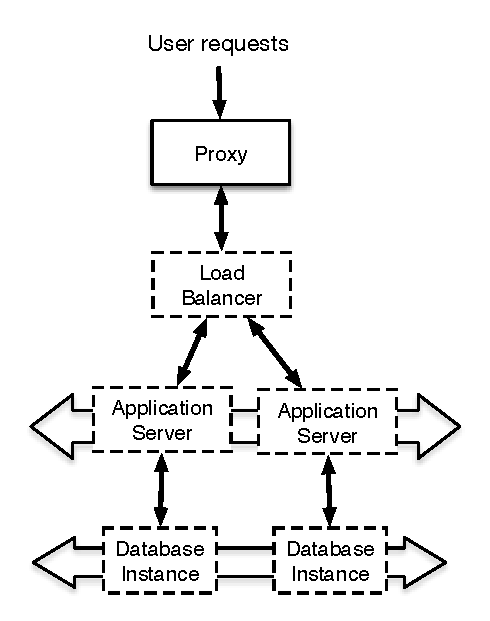
\includegraphics[width=0.35\linewidth]{images/architectureWithout}
}
\subfloat[b][with Shuttle]{
    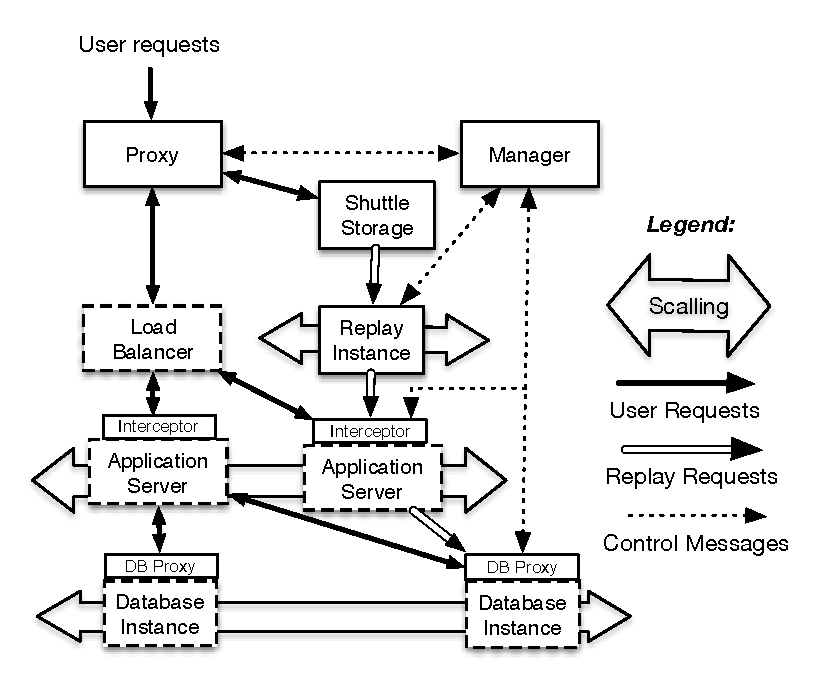
\includegraphics[width=0.55\linewidth]{images/architectureTiers}
}

\caption{Shuttle service architecture:The dashed line components are part of the \ac{PaaS} architecture. The proxy logs the user requests into the Shuttle storage. The manager coordinates the recovery process where the replay instances replay the user requests.}
\label{fig:shuttle_architecture}
\end{figure}
  

%Shuttle Storage
The \emph{Shuttle storage} keeps the content of the user requests and responses. Although we do not consider this aspect in the architecture, this store can be replicated to a remote site to allow tolerating catastrophic failures in a datacenter.


%trusted computing base
We consider the Shuttle components to be part of the trusted computing base since their integrity and availability are critical to recover the application state. We assume that intrusions tamper the application data, which is stored in the database, not the snapshots neither the stored requests. 

%Database
Unlike previous works, our design encompasses distributed databases (\acs{NoSQL}). These databases are designed to scale horizontally. Therefore, Shuttle can also be scaled by adding more database instances.

%How the architecture fits the PaaS
PaaS offerings are supported by a computing infrastructure, often provided as a service (IaaS model), able to scale the application allocating new instances on-demand or automatically, to maintain the quality of service despite demand oscillations. This elasticity  allows allocating replay instances and to scale the application to attend the requests issued by them during the recovery process. Due to the common pay-per-usage model, these resources are paid only when a recovery process occurs. The remaining cost of the service comes from storing client requests and database snapshots. Our design aims to optimize the available resources to reduce the recovery period and costs. 


%%%%%%%%%%%%%%%%%%%%%%%%%%%%%%%%%%%%%%%%%%%%%%%%%%%%%%%%%%%%%%%%%%%%%%%%%%%%%%%%%%%%%%%%%%%%%%%%%%%%%%%%%%%%%%%%%%%%%%%%%%%%
\section{Normal Execution}
\label{sec:arch:normal_execution}
Shuttle logs the data it needs to recover applications during the normal execution phase: user \ac{HTTP} requests, application \ac{HTTP} responses, database items accessed by each request and sequence of operations to each database item (Figure \ref{fig:normal_execution}). In this section, we describe the normal execution phase following the path that a request takes to be processed.

\begin{figure}
\centering
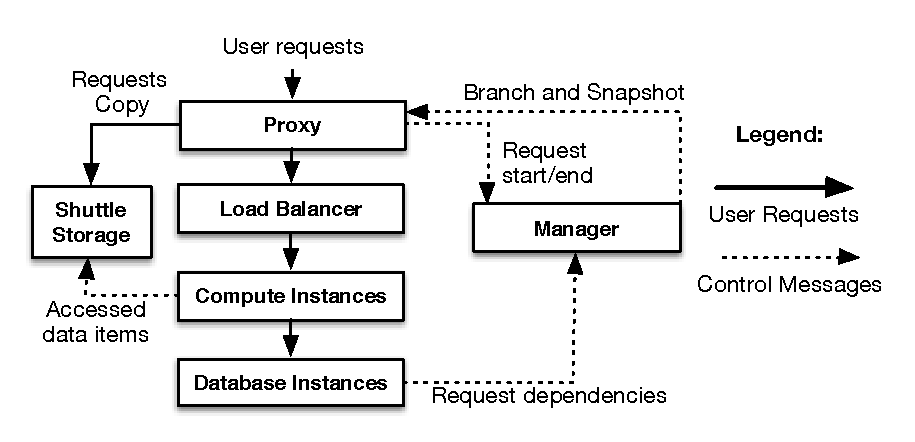
\includegraphics[width=130mm]{images/normalExecution}
\caption{Interaction between components during the normal execution}
\label{fig:normal_execution}
\end{figure}

%Proxy
The proxy intercepts all user \ac{HTTP} requests, except those to static contents (e.g., images), and adds a new header field named \ac{SRD}. Each \ac{SRD} contains three subfields: \ac{RID}, which is an unique timestamp; \emph{Branch} and \emph{Snapshot}, which define, respectively, the database branch and snapshot (Section \ref{sec:arch:snapshot}) and a \emph{restraint} flag, which is used to support runtime recovery (Section \ref{sec:arch:runtime_recovery}). 

The proxy also intercepts every application response, associates the response with the original request and adds a new timestamp to track the ending of the request execution. Requests, responses and their timestamps are stored in the \emph{Shuttle storage} using asynchronous I/O, which permits the operations to proceed before the transmission has finished. 

Requests are sent to the load balancer, which forwards the requests through the application instances according to their usage.


%Application instance
The application instances invoke the database service using the database client library. The database client library intercepts the operations, logs the accessed data items per request and stores this information in the \emph{Shuttle storage}. The database invocation is tracked at client side because the database may not be available or operations may fail.

%Database
On each database instance, the database proxy logs the operations' \ac{RID} and type. The sequence of operations to a data item defines its \emph{operation list}. Periodically, each database instance iterates the operation list of every data item to establish the dependencies between requests. Shuttle also performs snapshots periodically. The snapshot operation stores a new version of data item on the next write operation (Section \ref{sec:arch:snapshot}).


%Summary
In summary, every request-response pair is timestamped and logged by the proxy, the application instances the accessed data items per request, the database logs the sequence of operations per data item. The sequence of operations of each data item is kept in the database instance in which the data item is stored. The remaining data is stored in the \emph{Shuttle storage}, which can be located, or replicated, in a remote site to prevent catastrophic disasters rebuilding the application state using the requests and a previous snapshot. The manager retrieves, asynchronously, the requests' start and end timestamps, which are sent by the proxy, and their dependencies, which are collected by the database instances. Shuttle uses the information retrieved to generate the request dependency graph (Section \ref{sec:arch:dependencies}). 






%%%%%%%%%%%%%%%%%%%%%%%%%%%%%%%%%%%%%%%%%%%%%%%%%%%%%%%%%%%%%%%%%%%%%%%%%%%%%%%%%%%%%%%%%%%%%%%%%%%%%%%%%%%%%%%%%%%%%%%%%%%%
\section{Recovery}
\label{sec:arch:recovery}
%how we will recover?
The intrusion recovery process consists of three steps. The first step concerns the intrusion detection, in which tenants detect intrusions, suspicious behaviors or software flaws. Tenants may use automated tools such as \ac{IDS} \cite{itdb} to detect intrusions. The second step is vulnerability management in which vulnerabilities are identified, classified and mitigated. This work assumes that tenants identify the malicious requests (the subsequence of actions $A_{intrusion}$ whereby the attacker compromises the application) correctly and modify or remove them. Alternatively, tenants can provide an updated and vulnerability-free software version (Section \ref{sec:arch:detection}).
In addition, Shuttle provides several methods to help tenants to identify the malicious requests: determine the set of requests that accessed a set of affected database entries  after an estimated intrusion moment; group requests by user-session; compare database versions to check if the vulnerabilities are correctly mitigated.

The third step consists in removing the intrusion effects. Intrusions affect the application integrity, confidentiality and/or availability (Section \ref{sec:related:recovery}). Recovery from confidentiality violations is out of the scope of this document. However, we argue that the design of the applications should encompass cryptography techniques which may reduce data relevance and protect the data secrecy \cite{Maheshwari2000}.
Shuttle aims to recover applications from integrity violations, which often harm the availability. Shuttle can accomplish some of the goals of intrusion tolerance, keeping the application availability. Applications can keep providing a, possibly degraded but adequate, service during the intrusion recovery. Incoming requests are executed while the recovery process occurs without externalization to users (Section \ref{sec:arch:runtime_recovery}). In addition, Shuttle reduces the system downtime by reducing the time to recover when intrusions happen. Shuttle does not replace the intrusion prevention, detection and tolerance mechanisms, which are the primary lines of defense against attacks.\\

In order to remove the intrusion effects, Shuttle loads a database snapshot, which is selected by the tenant. The selected snapshot shall be previous to the intrusion moment in order to replace the value of every data item by a non-tampered value. Shuttle \textit{manager} orders the \ac{PaaS} controller to launch a new set of application instances and deploys an updated source code version, which may include code fixes. Then, the manager orders the database instances to load the selected snapshot (Section \ref{sec:arch:image_rejuvenation}). The application is intrusion-less now that the snapshot is previous to the intrusion and the application is redeployed on new instances. 

After, the manager initiates a set of \textit{replay instances} to replay the legitimate requests of the sequence of legitimate actions that happen after the snapshot, $A-A_{snapshot}-A_{intrusion}$. The replay instances retrieve a list of requests to replay and get the requests \ac{HTTP} package from the \emph{Shuttle Storage} (Figure \ref{fig:replay_execution}). Most \ac{PaaS} systems scale automatically and horizontally, i.e., they increment or decrement the number of containers based on the measurements of the containers usage. Therefore, the application-logic and data tiers scale to attend the requests from the replay instances, increasing the recovery speed.

The database separates the versions used by the replayed requests and the new requests, preventing the application from exposing a downtime. After the recovery process, the new requests are also forwarded to the recovered database version (Section \ref{sec:arch:runtime_recovery}).\\


The main version of Shuttle loads a previous database snapshot and replays every legitimate user request. An algorithm concerning selective replay is introduced in Section \ref{sec:arch:selective_replay}. \\

In the following sections, we discuss each of key process of the recovery phase in further detail.

\begin{figure}
\centering
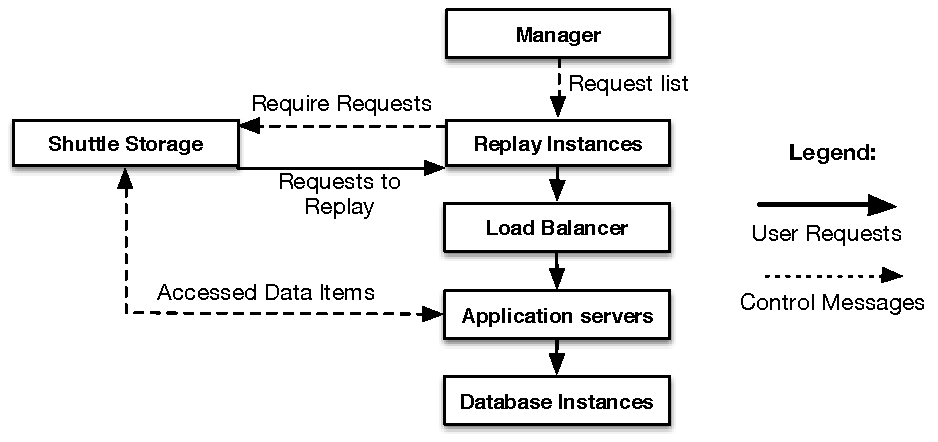
\includegraphics[width=110mm]{images/replayExecution}
\caption{Interaction between components during the recovery process}
\label{fig:replay_execution}
\end{figure}









%%%%%%%%%%%%%%%%%%%%%%%%%%%%%%%%%%%%%%%%%%%%%%%%%%%%%%%%%%%%%%%%%%%%%%%%%%%%%%%%%%%%%%%%%%%%%%%%%%%%%%%%%%%%%%%%%%%%%%%%%%%
\subsection{Intrusion and vulnerability correction}
\label{sec:arch:detection}
%how the damage is fixed?
The recovery process starts when intrusions are detected or the application software requires an update. Intrusion detection is out of the scope of this work. We assume that tenants, or system operators, detect one or more intrusions with the following sources:

\begin{enumerate}
\item User request (e.g. stolen user session)
\item External action: actions not logged by the proxy (e.g. ssh connection to the instances)
\end{enumerate}

Attacks may:
\begin{enumerate}
\item Tamper the database (e.g. adding new entries)
\item Tamper the container (e.g. changing the deployed application in the container)
\end{enumerate}

Shuttle supports the following actions to fix the exploited vulnerabilities:
\begin{enumerate}
\item Update the application software
\item Identify a set of tampered database entries
\item Add, modify or remove logged requests
\item Launch cleaned database or application server instances
\end{enumerate} 

Shuttle removes these effects of malicious actions redeploying the application in new containers and rolling back the database to a snapshot previous to the intrusion.

Attackers may use external actions to perform the intrusion, for instance gaining control of the instance to modify the database files. These actions are not recorded by Shuttle therefore they are not replayed and the application recovers a consistent state. We analyze several intrusion scenarios in Section \ref{sec:eval:accuracy}.\\


If tenants update the application software, they have to ensure that the application's interface remains compatible with the requests that will be replayed. Alternatively, tenants may update the entries in the database and provide a script to modify the requests make them compatible with the new \ac{API}. 

If the database is tampered using user requests, the tenant has to identify the malicious user requests. In addition,tenants can provide the set of suspicious database entries to Shuttle and it will resolve the set of requests that accessed the suspicious items after the estimated intrusion moment. Knowing the suspicious requests, the tenants shall use Shuttle to add, modify or remove the past requests to remove accidental or malicious behaves. \\

In summary, at the beginning of the intrusion recovery process, tenants shall ensure that:
\begin{enumerate}
    \item The software is correct: previous flaws are fixed, its \ac{API} is compatible with the requests and its behavior is the expected.
    \item The requests, which are selected to replay, are legitimate and their dependencies are correct.
    \item The estimated intrusion moment is previous to the intrusion moment (the selected snapshot is intrusion free).
\end{enumerate} 


%%%%%%%%%%%%%%%%%%%%%%%%%%%%%%%%%%%%%%%%%%%%%%%%%%%%%%%%%%%%%%%%%%%%%%%%%%%%%%%%%%%%%%%%%%%%%%%%%%%%%%%%%%%%%%%%%%%%%%%%%%%%
\subsection{Snapshot}
\label{sec:arch:snapshot}

%Why I need a snapshot? To reduce the work during replay.
Shuttle needs to remove intrusion effects. In Section \ref{sec:related:recovery}, we presented two mechanisms to do so: record the data item values or compensate the malicious actions. The first makes a copy of the data item value at a certain instant $t$, implying more storage resources. The second applies compensating actions to each action over the data item value after the instant $t$, which requires more computation resources to invert every action after $t$. However, the compensation mechanism requires the knowledge of the actions that revert the effects of the malicious actions. Moreover, if a malicious action is not recorded, then compensation mechanisms do not revert its effects. Since the set of operations is unknown and Shuttle aims to remove all intrusion effects, we perform snapshots by recording the value of the database items at a certain instant $t$ (first mechanism).\\

%What is a snapshot
A snapshot is a complete set of versions of every data item in the system from which data values can be read but to which updates are not made. Snapshots save the application persistent state at a certain moment. Unlike the selective undo approach, which only reverts the tainted data items (Section \ref{sec:arch:selective_replay}), the full replay approach loads a snapshot previous to the intrusion instant. This approach reverts every database item and removes the effects of any action that occurred after the snapshot creation. \\

%How it is useful?
The duration of the recovery process is mainly defined by the number of requests previous to the intrusion of the set, $A_{before}$. The snapshot mechanism avoids to replay every request from the beginning of the application, which can take too long. Shuttle requires not only a snapshot but also every action posterior to the snapshot instant. Therefore, Shuttle keeps every user request posterior to the oldest stored snapshot instant. The snapshot period defines the usage of storage and computation resources. We argue that tenants can balance the costs of storage and computation resources by specifying a policy to perform the snapshot. The policy shall consider the rate of requests, the data written per request, the expected time to detect the failure and the application capability to provide an possible degraded service during the recovery period. \\

%What Shuttle needs to do?
Shuttle takes snapshots automatically and according to specified policies. It records the persistent state of the application, i.e., the database values, at a certain instant. The volatile state of the application, for instance its stack, is not stored as we consider the web servers to be stateless. \\


%Request consistent snapshots
Performing snapshots in distributed databases is not trivial since snapshots have to be consistent with the user requests.  We consider each user request may include multiple database operations, each of them to multiple database servers, without using transactions. Consequently, the sets of database operations of each user request cannot be aborted and do not have a global order. If Shuttle replays requests on a snapshot that contains part of the persistent state written by a request during its first execution, the replay will be inconsistent. The database must reflect the effects of a set of completed requests and not the results of partially executed requests. Therefore each snapshot shall be \emph{global request consistent} containing either all or none of the database updates made by every request.


We define \textit{request consistent global snapshot}: a snapshot is global request consistent if it records a state of the database which reflects the effect of a set of completed requests and not the results of any partially executed request. This concept derives from the notion of \emph{transaction consistent global checkpoint}: a checkpoint is a transaction-consistent global checkpoint if it contains all or none of the updates made by a transaction \cite{global-checkpoint}. Since most \acs{NoSQL} databases do not support transactions, we extend the concept of transaction to \textit{request transaction}. A request-transaction embraces all database operations performed due to the execution of a request. Unlike \ac{ACID} transactions, a request-transaction may not be possible to abort. In summary, Shuttle snapshots are request consistent: a snapshot contain all or none operations of a request.


%Log-oriented vs dump-oriented vs Fuzzy
Checkpointing algorithms for distributed databases can be classified as log-oriented and dump-oriented \cite{checkpoint-survey}. In the dump-oriented approach, the checkpoint is referred to as the process of saving the state of all data items in the database. In the log-oriented approach, periodically a dump of the database is taken and also a marker is saved at appropriate places in the log. When a failure occurs, the latest dump is restored and the operations on the log after the dump was taken is applied to the dump until the marker is reached to restore the database to a consistent state \cite{global-checkpoint}. We take the latest approach.\\


In addition, the snapshot mechanism shall be non-blocking: the processes shall not stop their execution while taking snapshots.  

%Straightforward solution
A straightforward way to take a request-consistent global snapshot is to stop processing new requests, waiting until the currently executing requests finish, then making a copy of each data item. However, this solution incurs on communication overhead to reach a globally inactive state and causes application downtime. Yet, this approach may fit applications that can be unavailable during a certain period, for instance, during a certain period of the night. \\


Kim and Park \cite{kim_checkpoint} propose an approach in which a coordinator broadcasts a checkpoint-request message to every database node. Each database node divides the transactions into two groups: before the checkpoint-request $T_p$ and after $T_f$. Updates of transactions in $T_p$ are flushed to the current database, while the ones in $T_f$ are flushed in a \emph{checkpoint area} (a temporary allocated storage area). When all transactions of $T_p$ are done, the checkpoint area is updated with items updated by transactions in $T_p$ but not by $T_f$. After, the rules of current database and checkpoint area are exchanged. The major drawback of this approach comes from updating the checkpoint area: the database is unavailable during the updating process.


%Our solution
Our solution leverages the existence of a single load balancer and, consequently, single proxy that adds a \ac{SRD} field to every request. Every \ac{SRD} contains a \ac{RID}, an unique and incremental identification of each request given by the instant when the request is retrieved. Every database operation is identified by the \ac{RID} of the source user request.

In order to create a snapshot, tenants define a future instant in time $t$ when the snapshot will occur. The instant, named \ac{SID}, identifies the request-consistent global snapshot. The manager passes the \ac{SID} to every database proxy.

Database proxies use the \ac{SID} to define the version of the data item used by the operations. Operations with \ac{RID} lower than the scheduled snapshot instant (\ac{RID} < \ac{SID}) access the version before the snapshot. Otherwise, the operations access the latest data item version. This mechanism splits requests to accomplish a request-consistent global snapshot, and allows tenants to schedule snapshots without application downtime. Figure \ref{fig:snapshots} illustrates the sequence of 7 database operations on the database item $x$ and 3 snapshots (excluding the base snapshot).

\begin{figure}
\centering
  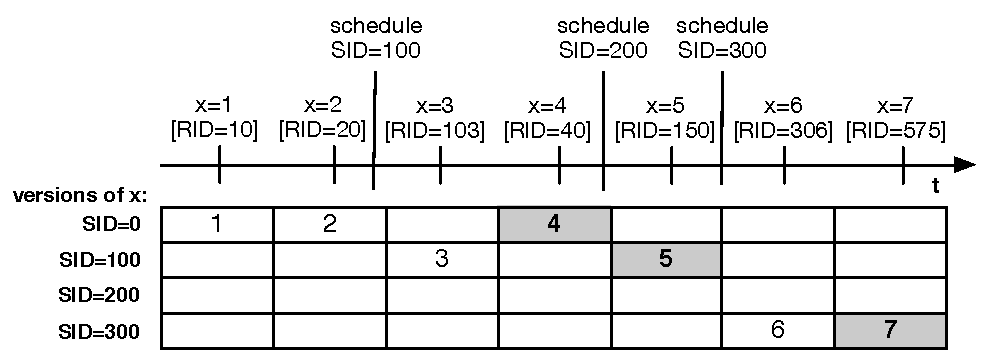
\includegraphics[width=130mm]{images/snapshots}
  \caption[Snapshot versions stored in the database]{Versions stored in the database during a sequence of 7 operations and 3 snapshots. The final values of the stored versions are contained in filled squares. The tenant schedules 3 snapshots on SID: 100, 200, 300.}
\label{fig:snapshots}
\end{figure}

In order to avoid to replay every database operation to obtain the snapshot, the snapshot mechanism shall create a database copy (dump). We avoid blocking the application to copy values using a copy-on-write and incremental method. When a data item is written for the first time in each snapshot, Shuttle creates a new version of the data item. Since a data item may not be written in every snapshot, e.g., $SID=200$ in Figure \ref{fig:snapshots}, we associate a \emph{version list} to every data item. A \emph{version list} tracks on which snapshots the data item has been written. In conclusion, the snapshot is an incremental mechanism because it does not require to duplicate data.\\
%The version list also contains read requests that did not succeeded, for instance when the data item does not exists, to avoid false positives. 


%Particular case
A snapshot might become inconsistent. For instance, Table \ref{tab:snapshot_caso_bicudo} represents the execution of two concurrent requests. Their normal execution is consistent. A snapshot with \ac{SID}=5 would contain [A1 = 11] and be a global request-consistent. However, if Shuttle loads the snapshot and replays the request 20, its first read operation reads A1 == 11 instead of A1 == 10. 


This particular case happens when a request with \ac{RID} greater than the snapshot instant \ac{SID} read a version belonging to the snapshot \ac{SID} and, after, a request with \ac{RID} lower than \ac{SID} overwritten that version. Storing a new version and adding a flag on the version list solves the problem. Nevertheless, we expect this to happen only in rare occasions.

%the  and every operation with \ac{RID} > \ac{SID} reads/writes the new version. Operations of requests with \ac{RID} > \ac{SID} that read the original value, for instance A = 10, are marked and read the old version during the replay. 
%in parallel during the transition period, i.e., when a request accesses the previous snapshot and other accesses the current snapshot. 


\begin{table}
\centering
\begin{tabular}{l|l|l}
\textbf{RID=10 (SID = 1)}     & \textbf{RID=20 (SID=15)}   & \textbf{Storage}\\ \hline
Write A=10                    & ~                          & A1=10  \\
~                             & Read A: A1==10             & A1=10  \\         
~                             & Write A=20                 & A1=10, A15=20 \\
Read A: A1==10                & ~                          & A1=10, A15=20 \\
~                             & Read A: A15==20            & A1=10, A15=20 \\
Write A=11                    & \textit{Completed}         & A1=11, A15=20 \\
\textit{Completed}            & ~                          & A1=11, A15=20 \\
\end{tabular}
\caption[Concurrent requests]{Concurrent requests: the snapshot instant is 15, the left request accesses data previous to the snapshot (A1) while the right accesses the latest (A15 or A1). }
\label{tab:snapshot_caso_bicudo}
\end{table}


%Discussion
Unlike the approach proposed by Kim and Park, our approach allows to record multiple snapshots keeping various data item versions and does not require to copy the transactions.

The value of \ac{SID} must be known by every database instance before the execution of any request with $RID > SID$. If the \ac{RID} was determined by incremental request counter, then Shuttle would need to analyze the request rate and estimate the \ac{SID} value. However, the request rate can vary and the snapshot would fail. Notice that our mechanism does not require clock synchronization because the \ac{RID} is defined by the proxy timestamp and tenants can schedule a snapshot defining a future time instant. The period between the scheduled moment and the present must be bigger than the communication delay between the manager and the database instances. Consequently, we assume the communication between the manager and database proxies is synchronous: the messages are delivered within a fixed time.


%%%%%%%%%%%%%%%%%%%%%%%%%%%%%%%%%%%%%%%%%%%%%%%%%%%%%%%%%%%%%%%%%%%%%%%%%%%%%%%%%%%%%%%%%%%%%%%%%%%%%%%%%%%%%%%%%%%%%%%%%%%%
\subsection{Dependency Graph}
\label{sec:arch:dependencies}
%Dependency definitions
An application execution can be modeled as a set of actions and a set of objects. Actions read and write objects. An action $A$ is dependent from an action $B$ if $A$ reads an object's version written by $B$.

%why is relevant in general
Requests must be replayed in a consistent manner to obtain a consistent application after the replay phase. The request replay order must ensure that if the requests, application semantics and initial database values are the same, then the final database values are equal. For this propose, the dependencies between actions shall remain consistent: if during the first execution an action $A$ becomes depends on an action $B$ by an object $O$, then during the replay phase $A$ shall read the object $O$ only after $B$ updates the object $O$. Otherwise, $A$ may read a version different than the original version.

%related work and why it does not work in PaaS
Previous proposals, for instance \emph{in} \cite{goel}, leverage the request serialization provided by snapshot isolation in relational \ac{DBMS} to order the operations to replay. In contrast, \textit{Undo for Operators} \cite{undoForOperators} uses the application protocol knowledge to establish the dependency between requests and order them. However, accesses to \acs{NoSQL} databases are not globally serialized. Moreover, the data items accessed during the replay phase may change due to updates to the application semantics, request modification or multi-threaded execution. At last, the application semantics is unknown in advance since we want to support any application deployed on \ac{PaaS}. Taking that into account, we propose a novel approach.\\


%Rules
Shuttle tracks the dependencies between actions in a \textit{dependency graph}. A \emph{dependency graph} consists of nodes that represent requests and edges that establish dependencies between them (Figure \ref{fig:selectiveGraph}).  Dependencies between requests are established using the following rules: a request $R_A$ is dependent upon request $R_B$ if there is a data item $x$ such that $R_A$ reads $x$ and $R_B$ performs the latest update on $x$ before the read operation by $R_A$. Dependencies are transitive except when requests perform blind writes, i.e., requests write items without reading them first \cite{Ammann2002}. Therefore, the dependency graph is a mixed graph, if there is a dependency between $A$ to $B$, then there may be a dependency between $B$ and $A$.


%How Shuttle creates the dependency graph?
Previous solutions for relational databases extract the dependencies using a pre-defined, manually-created, per-transaction type template \cite{itdb}, or change the relational database management system code to extract read dependencies \cite{phoenix}. In contrast, Shuttle uses the database proxy to log the database accesses. Periodically, each database proxy traverses, in background, the \emph{operation list} of each data item to collect the new accesses and to generate the dependencies between requests. The Shuttle manager processes the dependencies to update the dependency graph. An alternative approach is to pull the dependencies from each database node only before the recovery process and generate the dependency graph when needed. 






%false positives: detected but not exist
The above method may lead to \emph{false positives}, i.e., to flag dependencies that do not exist. For instance, a request may read a data item but not use it to compute the written value, so there is no real dependency. Although tracking variables used by each request during its execution might solve this particular case \cite{goel}, it would require modifying the code interpreter (e.g., Zend Engine for PHP), which would constrain Shuttle to a set of specific languages. As our approach uses the dependencies to group the requests that can be executed concurrently, false dependencies imply a performance penalty but do not cause data loss or inconsistent state. On selective replay mode, the dependency graph is used to determine the tainted requests and the request that need to be replayed. Again, false dependencies only harm the performance.

When tenants use the dependency graph to determine the set of malicious requests, $A_{malicious}$, they shall take into account that false dependencies may lead to consider legitimate operations as malicious and, consequently, cause data loss.

%false negatives: not detected but exist
Complex queries on a relational database may lead to \emph{false negatives}, i.e. a dependency exists but is not detected. For instance when a read operation would have been executed on a deleted data item if this data item had not been deleted before the request execution \cite{Xie2008}. Therefore, legitimate transactions may have different output even when they were not affected by malicious execution during their original execution. Since user mistakes are often delete operations due to wrong query arguments, this is a relevant issue. 

In contrast with SQL queries that access the data items that match a query, the \ac{CRUD} interface of most key-value stores specifies, in a deterministic and apriori manner, the data item that will be accessed. Shuttle logs every access, even when the data items do not exist, keeping the \emph{operation list} of the deleted data items to track further operations.\\


%Cycles
%Each request may perform multiple database operations, each of them to multiple database servers, without defining a global \ac{ACID} transaction. 
Shuttle can not replay requests synchronously, i.e., waiting for the response to the previous request before sending the next. To replay the requests synchronously would not have only performance degradation but also lock the replay phase because requests, which have been originally executed in concurrently during the normal phase, may be depend on each other. Therefore, Shuttle replays requests asynchronously and, hence, concurrently. Two requests are executed concurrently if they are dependent from each other. For instance, Figure \ref{fig:inconsistency_db_order} represents the first execution of two requests that increment the variable $A$. The $Request 1$ depends on $Request 2$ and vice versa. 

%Ordering using operation list
Yet, re-execution of concurrent requests is not deterministic. User requests are processed concurrently using multi-threaded servers and the system messages, including database requests, do not have a delivering order. Therefore, the execution order of two concurrent requests is unknown. To deal with this issue, our novel approach uses the \emph{operation list} to turn the re-execution of concurrent requests deterministic. An \emph{operation list} is a sorted list that records the operations to a data item. During the replay phase, the operations to a data item must follow the order established by is operation list. For instance, in Figure \ref{fig:inconsistency_db_order}, the operation list of the data item $A$ is: $[Req1:Get, Req1:Put, Req2:Get, Req2:Put, Req1:Get, Req1:Put, Req2:Get, Req2:Put]$. {Req.~1} and {req.~2} are replayed concurrently but the result is consistent because the order is established by the operation list.

%Unlocking
During the recovery period, intrusions are removed and the application code is updated. This may cause requests to access different data items than in the first execution. Requests may not access the same sequence of data items or read/write the same content. If an operation contained in the operation list is not performed, the following operations to the data item are blocked and the request fails. To address this problem, at the end of each request execution, the \textit{database client interceptor} fetches the list of data items accessed by the request on its first execution and compares them against the ones accessed during the replay process. The database client library invokes the \emph{database proxy} with the data items that have not been accessed to unlock the operations of the remaining requests. 

For instance in Figure \ref{fig:inconsistency_unlock}, the $Request 1$ has a different replay execution performing $B = B \times 5$ instead of incrementing $A$. The second operation of {req.~2} is delayed until the end of the {req.~1} because it succeed the second operation of {req.~1} in the operation list. After the execution of {req.~1}, the database client interceptor unlocks the second operation of {req.~2}.\\

\begin{figure}[!htb]
\hspace*{-3mm}
\mbox{
  \subfloat[][Ordered by the operation list \label{fig:inconsistency_db_order}]{
      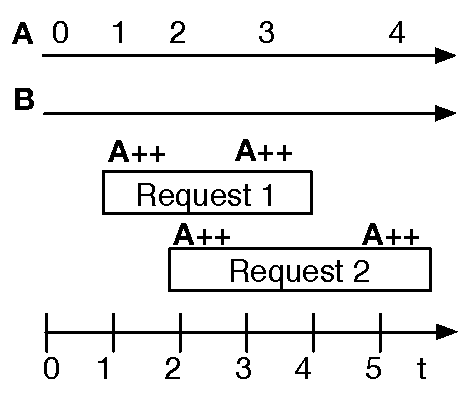
\includegraphics[width=0.25\linewidth]{images/inconsistency_db_order}
  }

  \subfloat[][Operation unlock \label{fig:inconsistency_unlock}]{
      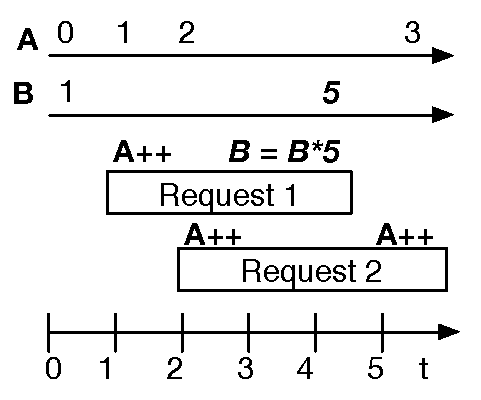
\includegraphics[width=0.25\linewidth]{images/inconsistency_unlock}
  }

  \subfloat[][Consecutive requests \label{fig:inconsistency_serial}]{
      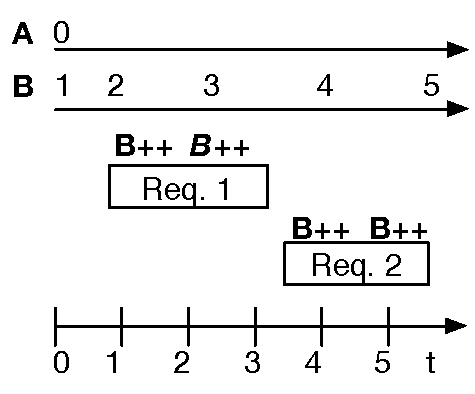
\includegraphics[width=0.25\linewidth]{images/inconsistency_serial}
  }

  \subfloat[][Conflict \label{fig:inconsistency_conflict}]{
      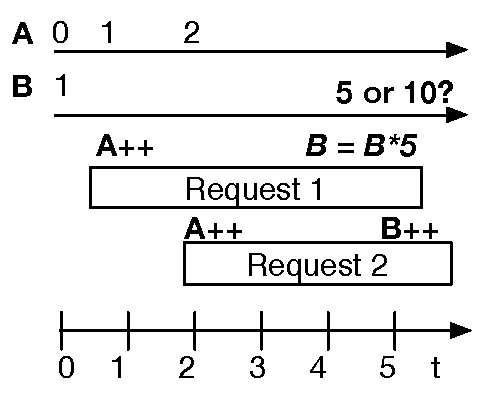
\includegraphics[width=0.25\linewidth]{images/inconsistency_conflict}
  }
}
\caption{Replay two requests with different re-execution}
\label{}
\end{figure}


%New dependencies during the recovery time
During replay there may be non-deterministic situations, whenever an access is not contained in the operation list. The most complex scenario during the replay is when two requests, originally executed in parallel, access different data items comparing with their first execution, establishing a new dependency. The result is unpredictable. Consider the possible re-execution in the Figure \ref{fig:inconsistency_conflict} where the {req.~2} increments $B$ simultaneously with {req.~1} performing $B = B \times 5$. The result is unpredictable because the {req.~1} may write before or after {req.~2}. Since both requests did not access the data item $B$ during their first execution, the operation list does not establish an access order. Therefore, the {req.~1} and {req.~2} may execute on a arbitrary order. The order of these requests is as deterministic as if during the first execution: the operation of \emph{req.~1} can execute before, between or after \emph{req.~2}.


%naive
A naive solution would be to detect the new dependency during the replay process, stop the process and start a new replay process in a new snapshot, including the new dependency.

%brown
Brown \textit{et al.} \cite{undoForOperators} propose the concept of \textit{verb} (Section \ref{sec:related:recovery_app}). A verb object encapsulates a single interaction (request/response) of the user and exposes an interface to establish the order between requests and their dependencies. However, tenants shall know the applications' operations to create the verbs defining: a commutativity test, an independence test, a preferred-ordering-test and an application-defined action to handle a inconsistency if the operation fails. Since Shuttle shall support any \ac{PaaS} application, the applications' semantics are unknown in advance. Therefore, this solution is not adequate.

%sorted log
A sorted-log, in which the accesses are sorted, for instance by \ac{RID}, would establish that operations must have a strict incremental order. However, operations with smaller \ac{RID} than the previous are aborted. For instance, the second operation of {req.~2} in Figure \ref{fig:inconsistency_db_order} would be aborted.

%sorting per start-end
An alternative solution consists on sorting the requests per \emph{start-end order}, instead of using the dependency graph. A request starts only after all requests with end lower than it ends. Dependencies between requests remain correct, since they are constrained by the \emph{operation list}. Thus the parallel requests are ordered and replayed in a similar manner to the first execution. Two serial requests can have distinct re-executions: if a request starts after the end of the previous. For instance in Figure \ref{fig:inconsistency_serial}, {req.~1} and {req.~2} can have distinct re-executions.

If two operations are re-executed concurrently, then their order is as deterministic as if they happen during the first execution. For instance in Figure \ref{fig:inconsistency_conflict}, the operation of {req.~1} $B = B \times 5$ is executed in parallel with the operations $B++$ of {req.~2}. The order of these requests is as deterministic as if during the first execution: the operation of {req.~1} can execute before, between or after {req.~2}.


%version and semantic reconciling
In order to turn more operations of the replay process consistent with the first execution, we can leverage semantic reconciliation, as \textit{in} Dynamo \cite{Decandia2007}. The case represented in Figure \ref{fig:inconsistency_conflict} is equivalent to a concurrent update where two parallel writes are performed on distinct database instances. Each request writes a distinct version resulting in conflicting versions of an item. Developers use the application-assisted conflict resolution interface to merge the versions (reconciliation) \cite{Decandia2007}. In this case, the following read operation would access the values written by the latest operation. For instance, if the latest is {req.~1}, then it choose between $1$ and $2$. If the latest is {req.~2}, then it choose between $1$ and $5$. This solution can produce a consistent output.\\

In summary, unlike previous solutions, Shuttle orders the requests using their start and end instants and constraining the operations to the order established on the \textit{operation lists}. This approach allows requests to access new data items during the recovery process and to replay concurrent requests.





%%%%%%%%%%%%%%%%%%%%%%%%%%%%%%%%%%%%%%%%%%%%%%%%%%%%%%%%%%%%%%%%%%%%%%%%%%%%%%%%%%%%%%%%%%%%%%%%%%%%%%%%%%%%%%%%%%%%%%%%%%%%
\subsection{Clustering}
\label{sec:arch:clustering}

Despite Shuttle's capability to replay concurrent requests, one of the main challenges of Shuttle is to reduce the recovery period. We assume that critical software flaws and intrusions can be detected in a short period of time, from seconds to one week. If a fault exists during a longer period, then the application may tolerate a longer recovery phase because the recovery process used by Shuttle does not require application downtime (Section \ref{sec:arch:runtime_recovery}). Still, we want recovery to take a fraction of the time elapsed since the snapshot from which recovery starts (e.g., if the snapshot was taken a week before, we want recovery to take much less than that period).  

We address this problem grouping the requests into \emph{clusters}. A cluster is a set of requests that have dependencies between them but not from/to requests in other clusters. Clusters are created when the recovery is about to start by inspecting the dependency graph. Since clusters are independent, they are executed concurrently by different \emph{replay instance} without synchronization. Requests within the same cluster, are performed in start-end order (Section \ref{sec:arch:dependencies}). Given that more requests are executed concurrently, Shuttle launches more application servers and database instances to process the replayed requests. Therefore, the replay phase throughput is bigger than the during first execution and the recovery time is minimized. This mechanism is applicable if the graph dependencies remain unchanged during the recovery phase, i.e,. every replayed operation is contained in the operation list but not all operations in the list must be replayed.

Taking the above in account, we define two replay approaches: \emph{serial replay} and \emph{parallel replay}. The first considers every request in the same cluster. The later uses the dependency graph to group the requests in independent clusters. Both approaches replay the requests in start-end order, supporting concurrent requests \ref{sec:arch:runtime_recovery}. In contrast to \emph{serial replay}, \emph{parallel replay} allows to perform more requests in parallel but it does not support new dependencies during the replay phase. Therefore, \emph{parallel replay} requires that tenants ensure that the dependencies between requests do not change during the replay process. Since the dependencies between requests often remain constant and novel dependencies are easily detected, we consider \emph{parallel replay} represents a significant advantage for \ac{CSP}. These approaches are compared in Chapter \ref{chapter:evaluation}.




%%%%%%%%%%%%%%%%%%%%%%%%%%%%%%%%%%%%%%%%%%%%%%%%%%%%%%%%%%%%%%%%%%%%%%%%%%%%%%%%%%%%%%%%%%%%%%%%%%%%%%%%%%%%%%%%%%%%%%%%%%
\subsection{Instance Rejuvenation}
\label{sec:arch:image_rejuvenation}

% Why? Instances can be corrupted
\ac{PaaS} systems launch instances/containers and deploy applications or databases on them. Attackers may exploit vulnerabilities in the instances configuration to affect the service integrity, confidentiality or availability. For instance, an attacker may explore the shellshock vulnerability in the GNU's bash shell of out of date instances.

%Related work
An effective technique to remove intrusion effects and restore the application availability is to terminate compromised containers and launch new containers. We name this approach as \textit{instance rejuvenation}. A similar approach is used in proactive recovery systems for Byzantine fault tolerance. Castro \textit{et al.} \cite{Castro2002} propose a mechanism that recovers the replicas of a system periodically even if there is no reason to suspect that they are faulty. This mechanism aims to prevent an attacker from compromising the service by corrupting a quorum of the replicas without being detected. We extend this approach to \ac{PaaS} to remove possible intrusion effects in containers, even if there is no reason to suspect that they are affected by the intrusion.\\



%How it works?
Shuttle interacts with the \ac{PaaS} controller rejuvenate instances when they are compromised and a new recovery process begins. This process launches new instances. The \ac{PaaS} controller initializes the new instances with updated container images and deploys an updated version of the application code or database, which may include updates to fix discovered flaws or prevent future intrusions. Shuttle copies the snapshot selected by the tenant to new database instances. Requests are replayed on the novel instances while the incoming requests are processed by the old instances, perhaps with a degraded integrity constrains. This mechanism keeps the application available during the recovery process. After the recovery process, the old instances are terminated.\\

%Why its good?
We assume new instances to be intrusion-free since tenants or CSPs can update the image and the image is installed on an empty persistent-state. This approach fits the concept of automatic deployment applications in \ac{PaaS}. Applications for \ac{PaaS} platforms are designed to scale horizontally so the number of application instances can be dynamic.

%remote replication
In addition, the instances can be instantiated in a remote site to recover from catastrophic disasters \cite{cloud-disaster}. Snapshots, database operation lists, application code and requests can be replicated to a remote site. If they are available, then Shuttle can launch new instances on a remote datacenter, deploy the application code, load the snapshot and operation lists in the database instances and replay the requests. This is a log-based recovery process \cite{Wang2010} that allows to recover the  application integrity and availability.

%software testing
This process can also be used in a proactive manner to renew instances to remove unknown intrusions \cite{Castro2002,Sousa2010} or to test new application versions with user requests to compare its results against the previous version, using the branching mechanism  (Section \ref{sec:arch:runtime_recovery}).

%Consistency
Tenants are responsible for ensuring that request dependencies are correct and the {API} of the updated code version is compatible, or for providing a script to update each request to the new \ac{API}. Moreover, the selected snapshot must be consistent according to the specification of the updated version or every request executed since the application begin shall be replayed.



%%%%%%%%%%%%%%%%%%%%%%%%%%%%%%%%%%%%%%%%%%%%%%%%%%%%%%%%%%%%%%%%%%%%%%%%%%%%%%%%%%%%%%%%%%%%%%%%%%%%%%%%%%%%%%%%%%%%%%%%%%%%
\subsection{Runtime Recovery}
\label{sec:arch:runtime_recovery}

%Goal
Applications shall remain available during the recovery process, perhaps with a degraded behavior, without exposing downtime to users. To do so, Shuttle considers each recovery process defines a new branch, a model inspired in versioning systems such as git \cite{git}.

%How
A \emph{branch} is a sequence of snapshots. Snapshots are analogous to \textit{commits} in git. Each snapshot represents a set of versions of every data item in the database at a certain instant. Each recovery process creates a new branch forking a previous branch on a snapshot chosen by the tenant, either explicitly or implicitly (by indicating the initial intrusion instant, selecting implicitly the preceding snapshot). When a new branch is created, a new snapshot is also created on the new branch. Incoming user requests access only the data of the previous branch keeping the application available, while replayed requests access the created branch without compromising the availability of the application. If Shuttle launches new database instances, then the new branch is created in the new instances and write operations occur in the new instances. Read operations occur in the previous instances until the first write operation of the accessed data item in the new instances.

\begin{figure}
\centering
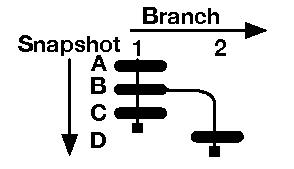
\includegraphics[width=55mm]{images/branches_paper}
\caption[Tree model]{Tree model: 2 branches and 4 snapshots: branch 1 contains the snapshots $A, B, C$; branch 2 contains the snapshot $D$;}
\label{fig:branches_simple}
\end{figure}


%Architecture details
A branch contains a sequence of snapshots but a snapshot can only belong to a single branch (Figure \ref{fig:branches_simple}). Each snapshot represents a possible version of the data item. A novel data item version is created only when the data item is written for the first time during each snapshot. Consequently, the data item may not have a version for each snapshot. Shuttle keeps a list of the versions in which each database item has been written (Section \ref{sec:arch:snapshot}).

%Problem of lack of versions:
For instance, in Figure \ref{fig:branches}, a data item $x$ may have the following sequence of versions on its version list: $[A,B,C,D,E]$. If $x$ has not been written in snapshot $E$, the version $E$ would not exists and the latest version of $x$ would be $D$. However, the snapshot $D$ has been compromised so it is not part of the current branch (branch 3). The latest non-tampered version of $x$ is the version $B$. If version $B$ does not exists, then the latest version is $A$.

%branch path
We define the concept of \emph{branch path}:  a Branch Path of a certain branch is the sequence of snapshots between the current snapshot and the root snapshot. A Branch Path of a certain branch defines the versions available to operations that belong to that branch. The branch path of branch $3$ in Figure \ref{fig:branches} is \{E, B, A\}. The one of branch $2$ is: \{D, C, B, A\}. When a branch is created, its branch path contains the its initial snapshot and the sub-sequence of snapshots in the branch path of the branch of the forked snapshot that are equal or previous to the forked snapshot.

%Version to read
The version accessed by an operation is defined using the branch path of the operation's branch and the version list of the accessed data item: operations read the latest version present in the \emph{version list} and in the \emph{branch path} and write the latest version in the branch path. Therefore, a new version, referring the initial snapshot of the new branch, is added to the version list on the first write operation to each data item during the replay.

%Isolation
This mechanism maps the operations to the correct versions and isolates the multiple, perhaps simultaneous, attempts to recovery the application without compromising the exposed application behavior. During the recovery process, users access the, perhaps corrupted, old branch loaded in the current computation and database instances. Therefore, the application remains online, perhaps with a degraded behavior, without exposing downtime to users.

%Working explanation and switching
At recovery time, the manager sends the new \emph{branch path} to every database instance. The new incoming users access the, perhaps corrupted, old branch while the requests being replace access the new branch. Therefore, the application remains online, perhaps with a degraded behavior, without exposing downtime to users. 

At some point, when the recovery is finishing, the user requests have to start being issued to the new branch. To do so, after replaying the requests, the proxy flag \emph{restraining} is set and every new request is marked with the \emph{restrain} flag. Database accesses marked with \emph{restrain} are delayed. After replaying the requests retrieved during the recovery process, the proxy sets the new branch in the subfield \emph{branch} of \ac{SRD} of the new requests, the \emph{restrain} flag is disabled and the database nodes are notified to proceed the accesses. This mechanism delays the processing of some requests, but this has typically a duration of seconds, compared with a recovery process that may take many minutes or even hours. 

This mechanism ensures the recovery phase to be finite. However, if the rate of requests being replayed is much higher than the rate of new requests, then the requests retrieved during the replay phase are also replayed without restraining new requests. Consequently, the restrain phase is shorter and required only to change branch. 

%Related work, advantages and example
While Aire \cite{retro} used a branching mechanism to perform a recovery process in various systems simultaneously, we propose the mechanism to isolate user accesses from the recovery process. Our model allows the tenants to select any snapshot as base to a new recovery process and create snapshots in different branches. Applications can contain multiple branches simultaneously. Figure \ref{fig:branches} represents an application with 3 branches: the branch 1 is the initial application branch where the tenant made three snapshots ($A$, $B$ and $C$). After detecting an intrusion, the tenant considered that snapshot $C$ is non-tampered and initiated a recovery process based on it creating the branch 2. Afterwards, the tenant made one snapshot ($D$) on branch 2. However, the snapshot $C$ is tampered. So the tenant initialized a novel recovery process based on snapshot $B$ creating the branch 3. In this scenario, the tenant would be unable to recover its application without the branching model. Since tenants may fork a new branch not only from the most recent snapshot. Therefore, the latest non-tampered version of a data item may not be its latest version.

\begin{figure}
\centering
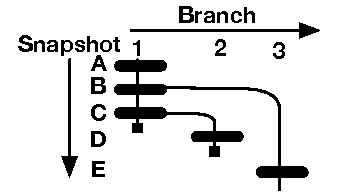
\includegraphics[width=65mm]{images/branches}
\caption[Tree model]{Tree model: 3 branches and 5 snapshots: branch 1 contains the snapshots $A, B, C$; branch 2 contains the snapshot $D$;  branch 3 contains the snapshot $E$.}
\label{fig:branches}
\end{figure}



Inactive snapshots and branches, for instance snapshot $D$ and branch 2 in Figure \ref{fig:branches}, can be deleted to reduce the used storage resources. In addiction, tenants can use the branching mechanism to test their intrusion recovery procedures in background, i.e, without exposing users to test issues.\\

If an intrusion happens during the replay phase, then its effects are stored in the branch of incoming requests. If the intrusion is detected before the restraining flag is set, then the malicious requests are not replayed in the new branch. Otherwise, tenants shall start another recovery process.\\





%%%%%%%%%%%%%%%%%%%%%%%%%%%%%%%%%%%%%%%%%%%%%%%%%%%%%%%%%%%%%%%%%%%%%%%%%%%%%%%%%%%%%%%%%%%%%%%%%%%%%%%%%%%%%%%%%%%%%%%%%%
\subsection{Non-determinism and consistency}
\label{sec:arch:consistency}

Shuttle provides an \ac{API} to handle nondeterminism and inconsistency cases.

%non-determinism: definition
An application is called nondeterministic if two subsequent executions with the same user input cannot be guaranteed to have the same have the same final state and outputs. Five of the main sources of non-determinism in \ac{PaaS} applications are: shared memory, thread concurrency, random number generation, timestamps and message exchanging.

%how non-determinism is handled
We assume requests to be independent thus they do not share memory and concurrent threads are independent. The \ac{API} of Shuttle provides a deterministic random number generation and a timestamp. It uses the \ac{RID}, which is a timestamp set by the proxy, as timestamp and pseudo-random number seed, so the replay of a request will use the same random numbers and timestamp. We consider a single timestamp per request to be enough for most applications. This mechanism is language independent. User requests and database accesses are ordered in a deterministic way using the operation list. Shuttle provides the following \ac{API} for the application developers:

\begin{enumerate}
  \item \textit{getTimestamp():} returns the timestamp (\ac{RID}) set by the proxy (\textit{long}).
  \item \textit{getRandomGenerator():} returns a random number generator that has \ac{RID} as seed.
\end{enumerate}

%User consistency
An important aspect of a recovery system like Shuttle is the application consistency seen by users. For instance, if an user does an action based on data written by a malicious action, which result of the user action replay is consistent. Since users have a non-deterministic behavior, they may have to be notified if a recovery took place and their data was modified. \\


%Related work
%In Undo for Operators \cite{undoForOperators}, operators must specify a compensation action for each request type. 
Since Shuttle is not tied to the application semantics, the actions to compensate the recovery process changes are unknown before the application is created. In addition, the application may contain client-side code, e.g., Javascript, that processes the application responses. For instance, a recover process reorders a list of items. The client-side code may sort the items so the list is seen ordered by users. A replay process taking into account the client-side consistency is proposed in \cite{warp}.


% Compensation API
Shuttle does not execute requests that returned an error in the first execution. We assume that requests are synchronous so users are immediately notified of the error and do not expect that the request will succeed in future. Similarly to other works in the area \cite{undoForOperators}, we assume that these cases are compensated by the user when they happen. As only requests that did not return an error are replayed, Shuttle considers an inconsistency when a request returns an error or a response is different during replay. Shuttle provides the following \ac{API} for the application programmer to define how inconsistencies are dealt with (Shuttle calls these functions in case they are launched by the tenant):

\begin{enumerate}
  \item \textit{preRecover():} invoked before the beginning of the recovery process.
  \item \textit{handleInconstency(request, previous response, new response, previous data items, new data items, action):} invoked when there is an inconsistency.
  \item \textit{postRecover(statistics, old version, new version):} invoked after the end of the recovery process.
\end{enumerate}

The first function allows tenants to perform a set of actions before the beginning of the recovery process, such as notifying the operations team or taking a new snapshot. 
The second function takes as input the operation that caused the inconsistency as well as the response and keys accessed during the normal execution and during the recovery process. It also takes as argument the action to take. Currently we consider three possible actions: 1) ignore the inconsistency; 2) notify the user of the inconsistency; 3) execute another request. This function is invoked, for instance, if a response during the replay is different than the response on the first request execution.
Using the \textit{postRecover} function, the tenant has access not only to the statistics of the recovery process but also to an interface to compare the database values before and after the recovery process and the application responses, before exposing the data to the users. 
Tenants can use this interface to notify their customer to verify their data.
%If tenants aim to determine if a request returned an error in the first execution due to an intrusion, Shuttle can replay the failed requests too.

%External consistency
Besides its users, an application may also interact with external services. We simplify the problem by considering that applications only obtain inputs from external services, disregarding the issue of outputs. The problem is treated in \cite{undoForOperators,aire}. Brown \textit{et al.} \cite{Brown_spheres} models each external service as a recoverable application. During the recovery phase, an external service can also be recovered if its input is distinct. Aire \cite{aire} proposes to initiate a recovery process in the external service and handles the inconsistencies of this process.


%%%%%%%%%%%%%%%%%%%%%%%%%%%%%%%%%%%%%%%%%%%%%%%%%%%%%%%%%%%%%%%%%%%%%%%%%%%%%%%%%%%%%%%%%%%%%%%%%%%%%%%%%%%%%%%%%%%%%%%%%%%%
% \subsection{System Administrator Support}
% \label{sec:arch:system_admin_support}

% Shuttle aims to facilitate the recovery process aiding the tenants to recover their applications from intrusions. Shuttle helps the tenant to identify the malicious requests based on: 
% \begin{enumerate}
% \item tainted responses;
% \item the requests that accessed a set of data items;
% \item per user, per user session, per ip-range
% \end{enumerate}
% %    \hl{a maquina que foi afectada, tracking do codigo que foi actualizado, etc ha muitos criterios possiveis}.

%  It also displays the requests dependency graph. It allows the tenant to preview the results of the recovery process without exposing them to the users. It provides a database version compare tool to check if the vulnerability is correctly mitigated.
% \hl{apago esta secção?}

%%%%%%%%%%%%%%%%%%%%%%%%%%%%%%%%%%%%%%%%%%%%%%%%%%%%%%%%%%%%%%%%%%%%%%%%%%%%%%%%%%%%%%%%%%%%%%%%%%%%%%%%%%%%%%%%%%%%%%%%%%%%
\subsection{Full and Selective Replay}
\label{sec:arch:selective_replay}

%Full vs selective goals
We propose two approaches for intrusion recovery: full replay and selective replay. Full replay consists in replaying every request done after the  snapshot. Executing many requests takes considerable time, so this approach is adequate for intrusions detected reasonably fast after they happen, e.g., a few days. 


%Explain
Selective replay (Section \ref{sec:related:recovery_models})  re-executes only part of the requests so it is faster than full-replay. However, it requires tenants to provide a set of malicious actions (i.e., requests) $A_{intrusion}$. This set is used to deduce the set of tainted requests $A_{tainted}$. A request is said to be tainted if it is one of the attacker’s requests or if it reads objects written by tainted request \cite{taser,itdb,phoenix}.  

%Tait
Tainted requests can also be determined by Shuttle considering the tampered data items and an estimated intrusion moment. Selective replay approach loads only the previous versions of the tainted objects, $O_{tainted}$, and replays only the legitimate operations, which were tainted, $A_{tainted} \notin A_{intrusion}$, to update the application persistent state. Selective replay, as compensating actions, does not remove the effects of unlogged actions because their dependencies are unknown. 

%related work
In \cite{goel,retro}, the set of tainted operations, $A_{tainted}$, is determined using \textit{taint propagation via replay}. To do so, they load a previous version, from a snapshot, of the objects in $O_{intrusion}$. Then, the actions, which are dependent from the restored objects, are replayed and their output objects are updated. The forward actions, which depend on the updated objects, are also replayed while their inputs are different from the first execution. The propagation is done thought the output of actions with different execution.
Unlike these approaches, Shuttle does not store the input and output of every action, i.e., database operation. Shuttle proposes an approach in which the requests are replayed, at least, until the first snapshot after the selected snapshot. Consequently, the application semantic must remain unchanged, i.e., the same request and same input must perform the same write operations. Otherwise, the dependencies between requests are unpredictable and the tainted requests can not be determined. An approach that allows to update the application semantics is proposed in \cite{warp}. We consider storing all versions of a data item has prohibitive storage costs for enterprise applications.\\

%Which requests are replayed?
For instance, consider the dependency graph of Figure \ref{fig:selectiveGraph}, in which every request reads a data item and writes a new value on the same data item. The request $4$ was identified as a malicious request. Therefore, requests $5,6,7,8$ are tainted. Since Shuttle does not keep every version of the entries, the value read by request 4 is unknown. In order to get this value, Shuttle must replay the {req.~2}, which wrote the value read by {req.~4}. The value read by request 2 is known because Shuttle performed the checkpoint A. Since the application semantics remains the same and its input is known, {req.~3} does not need to be replayed. Requests $5,6,7$ are replayed since they depend on the malicious {req.~4}. Values read by request 8 are known due to checkpoint B. Therefore, {req.~8} may not be executed if the value of the data items remains the same. Shuttle performs \textit{taint via-replay}: if a request writes in a data item which were not written previously, then the requests which read or write that data item, are also replayed. For instance, the {req.~9} may read a data item written by the {req.~4} during the replay but not during its first execution.\\


\begin{figure}
\centering
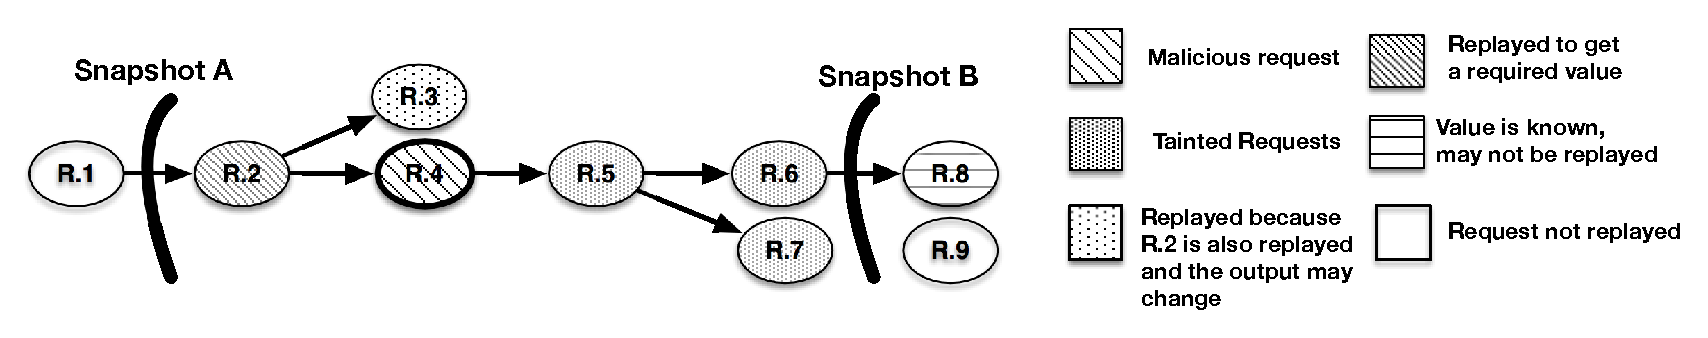
\includegraphics[width=150mm]{images/selectiveDependency_legended}
\caption[Dependency graph]{Dependency graph: $R.1$ is previous to a snapshot $A$; $R.3$ is dependent on $R.2$, which is replayed to get the read values; $R.4$ is a malicious request; $R.5,R.6,R.7$ are tainted; $R.8$ may not be replayed; $R.9$ is independent of the rest}
\label{fig:selectiveGraph}
\end{figure}

The selective replay process is as follows (full replay is simpler so we skip it):
\begin{enumerate}
\item \textit{Determine the malicious requests $A_{intrusion}$.}
Based on initial data such as user session compromised or data items accessed or other criteria, the tenant determines the requests $A_{intrusion}$ used by the attacker to compromise the application. For instance, $A_{intrusion} = \{R.4\} $ in Figure \ref{fig:selectiveGraph}.

\item \textit{Use $A_{intrusion}$ to determine the set of tainted requests $A_{tainted}$.}
For each request in $A_{intrusion}$, traverse the dependency graph in causality order and add these nodes to $A_{tainted}$ (in the figure $A_{tainted} = \{R.5,R.6,R.7,R.8\}$).


\item \textit{Get the requests needed to obtain the values read by $A_{tainted}$ and their effects.} 
Instead of storing the input and output of every action or versions of every data item, we propose to replay the actions which $A_{tainted}$ depends on. The data item value is known at the snapshot instant so the algorithm transverses the graph in inverse causality order from each request in $A_{tainted}$ and stores the requests in $A_{replay}$ ($A_{replay} = \{R.2\} \cup A_{tainted}$). $A_{replay}$ is expanded by traversing the graph from each of its elements on causality order to determine the requests which can be affected by the re-execution of $A_{replay}$ ($A_{replay} = A_{replay} \cup R.3$). Requests subsequent to the first snapshot after the latest malicious request may not be repeated as the data item version is known (version read by $R.8$ is stored in snapshot B).

\item \textit{Determine the replay order.} 
The set $A_{replay}$ is sorted on non-clustered \emph{start-end order}.

\item \textit{Load the previous data item versions}
Shuttle loads the version in the selected snapshot of the data items read by the requests in $A_{replay}$ and written by $A_{malicious}$.

\item \textit{Replay the requests}
Requests in $A_{replay}$ are replayed. If an access is not contained in operation list, then a new dependency is established and the requests that accessed the data item during the first execution are also replayed as in \emph{taint propagation via replay} \cite{retro}. For instance, $R.9$ is replayed if it reads an item written during recovery process but not during normal execution. 
\end{enumerate}

%merging branches
%After replaying the tainted requests, Shuttle compares the branches. \hl{ver se isto é necessário, na prática pode carregar apenas os dados novos}
% Depois para fazer o merge: compara as branches indo de key em key e comparando o hash dos valores guardados. As combinações são:
% |  Old  |   Recuperada |
%    A            A           - (sao iguais) - está tudo bem, um algoritmo de compressão pode colocar ambas as versões a apontar para o mesmo valor
%    -            B           - (nova entrada) - A versão recuperada ganha
%    A            B           - (modificado) - A versão recuperada ganha

% As entradas recuperadas escrevem sobre as que existem. Neste caso, os items apagados são também apagados.


 %A eficacia e melhoramento do selective replay depende do numero de entradas afectadas. Um simulador foi implementado e os resultados sao apresentados nos testes.

 Shuttle does not require generating a dependency graph in non-clustered full replay mode. The dependency graph is required in the case of clustered full replay to identify the independent clusters of requests and on selective replay to determine the tainted requests. We use the database operation lists to create the dependency graph and to order the execution of parallel requests without knowledge of the application protocol. 
 
 In summary, the selective replay approach reduces the number of requests to be replayed during the recovery process but implies that the application remains unchanged and does not revert the actions performed by unlogged requests. 


%%%%%%%%%%%%%%%%%%%%%%%%%%%%%%%%%%%%%%%%%%%%%%%%%%%%%%%%%%%%%%%%%%%%%%%%%%%%%%%%%%%%%%%%%%%%%%%%%%%%%%%%%%%%%%%%%%%%%%%%%%%%
\section{Chapter Summary}
\label{sec:arch:summary}
Shuttle recovers from security intrusions loading a previous snapshot and replaying the legitimate requests. It uses database snapshot and clustering to reduce the recovery time. Shuttle leverages the pay-per-usage model of \ac{PaaS} to provide a cost-efficient and fast recovery service instantiating the replay instances and more application containers on demand during the recovery process. \\

Shuttle proposes two approaches to perform replay: selective replay and full replay. 

\begin{table}[h]
\centering
    \begin{tabular}{l|ll}
               & Clustering & Non-Clustering \\ \hline
    Selective &  \xmark     &  \cmark        \\
    Full      &  \cmark     &  \cmark             
    \end{tabular}
\caption{Shuttle Replay modes}
\label{tab:operation_types}
\end{table}

The full replay approach supports parallel re-execution of requests that belong to independent clusters (clustering). Clustering is not supported on selective replay because the \textit{taint propagation via replay} defines the set of requests to replay at running time. Clustering is not supported with selective replay because taint propagation via replay defines the set of requests to be replayed in runtime.

The decentralized applications are more vulnerable to failures because of the single proxy architecture. However, we argue that future architectures can consider replication of the proxy, load balancer, Shuttle Storage and database. 
\cleardoublepage
\phantomsection
%!TEX root = ../tese.tex
%!TEX encoding = UTF-8 Unicode
\chapter{Implementation}\label{chapter:implementation}
This chapter addresses the main decisions adopted regarding the implementation of the intrusion recovery system Shuttle. Shuttle is supposed to be implemented by the \acf{PaaS} providers since it requires modifications to the \ac{PaaS} system and database service.

%button-up approach. What are the base technologies?
\section{Adopted Technologies}\label{sec:impl:adopted_technologies}
%Criteria
In order to implement the proposed work, we evaluated several technologies taking in account the requirements of the problem and the performance, scalability and easiness of implementation in a production mode \acf{PaaS} provider service.
%Python
The first Shuttle prototype was implemented in Python. The prototype of a simple application and the proxy allowed to analyze the requirements of Shuttle. The compact code of Python was great for code readability and rapid prototyping. However, despite the stackless variants of Python, the global interpreter lock limits Python to a single active thread per process. Since all modules of Shuttle are multi-threaded and their performance is critical to support medium and large-scale systems, Python was not appropriated. The selected language needs to be likely to run faster than Python and to have better concurrency and network libraries.

%C and C++
C or C++ languages are likely to have a better performance than Python because they are compiled to assembly. However, the development time can be considerably larger due to its low level. 
Java has an higher abstraction level than C but lower than Python. To argue about the performance differences between Java and Python, we would need to develop a version of Shuttle in Python and another version in Java. However, the proxy prototype using Java has a bigger throughput and lower latency than the one implemented using Python. 

%Scala, Go, Erlang
Shuttle has a distributed architecture and each module shall process various requests concurrently. Therefore, we also considered languages, such as \emph{Erlang}, \emph{Go Lang} and \emph{Scala}. They facilitate the writing of concurrent programs that share the state by communicating. Moreover,the actors model \cite{actors}, native in Erland and available through frameworks as Akka \cite{akka} to Scala, could simplify the implementation and improve the performance. 

%Java
Since the selected database is implemented in Java (Chapter \ref{sec:impl:database_options}) and Java is still the most used language in enterprise environments and it is compatible with most of \ac{PaaS}. In addition, Java has a \acf{NIO} library that provides event-driven and asynchronous communication via network. Due to its broad usage, Java is more likely to have client libraries for distributed databases than other languages, for instance C.

%Why not Java?
We chose to implement the Shuttle prototype in Java. However, the large number of concurrent tasks and asynchronous message passing communications turned the development of the prototype using Java extremely complex. Moreover, it's concurrency model and network libraries have an abstraction level lower than desired to archive a fast development and good performance.

Therefore, during the development of the prototype, we concluded that \emph{Scala} with \emph{Akka} could be a better option than Java. It would be likely to simply the development of the distributed system and improve the performance. However, rebuilding the prototype in a different language would also take too long. Therefore, we kept Java. \hl{sei que é atipico na tese dizer isto mas prefiro ser honesto... java para este tipo de coisas simplesmente não presta.}
In addition, the proxy performance could be improved using a C or C++ implementation, such as in \cite{haproxy}. \\

Despite the Java \acf{RMI} \ac{API}, we choose to use a messaging protocol because Shuttle is built of several modules that communicate and coordinate their actions by passing messages. The message passing protocol should emphasized simplicity, performance and low overhead. It should also define data structures and service interface easily. 

Plain text protocols is a communication protocol whose content representation is intended to be read by humans. For instance, \acf{SOAP} \cite{soap} specifies rules for using XML to package messages. Despite the heterogeneity and easiness of debug of plain text protocols, the text encoding and message structure has a significant overhead. As opposed, binary protocols are intended to be read by machines. The advantage of terseness translates into smaller messages and faster transmission and interpretation than plain text protocols. The capability of describe data structures using a \acf{IDL} and generate the source code in various programming languages to generate and parse the stream of bytes is also important to reduce the period of implementation and support transparent interaction between multiple programming languages. To cope with these requirements, we selected a binary protocol with \ac{IDL}. 

Apache Thrift \cite{Thrift} and Google's Protocol Buffer \cite{protobuffers} are two of the current binary communication protocol that fit these requirements. These protocols are similar, the main difference is the first offers a stack implementation for \acf{RPC} calls. The exact performance differences between them can only be measured benchmarking the two possible implementations. We choose Protocol Buffers to implement our prototype.



%%%%%%%%%%%%%%%%%%%%%%%%%%%%%%%%%%%%%%%%%%%%%%%%%%%%%%%%%%%%%%%%%%%%%%%%%%%%%%%%%%%%%%%%%%%%%%%%%%%%%%%%%%%%%%%%%%%%%%%%%%%%%
\subsection{Platform as a Service}\label{sec:impl:paas}
Shuttle is implemented as a service in \ac{PaaS} framework. Since we can not modify the implementation of \acf{CSP} solutions, such as Google App Engine \cite{GoogleAppEngine} and Amazon Web Services \cite{AmazonElasticBeanstalk}, we chose an open-source \ac{PaaS} framework. The framework must meet the following requirements: 

\begin{enumerate}
	\item \textit{Open-source:} to support updates and modifications
	\item \textit{Support to add new containers (auto-scaling is not mandatory):} to add new compute, database and replay instances.
	\item \textit{Contain a load-balancer:} to distribute the requests after the proxy
	\item  Extensible to support a new database management system
	\item Deployable on OpenStack and \acf{AWS}
	\item Support for Java Applications
\end{enumerate}

We consider the auto-scaling capability as optional since Shuttle may invoke the \ac{PaaS} manager to create new web-servers, database instances and replay instances. However, the capability to monitoring the containers usage during the recovery period turns the replay process faster and cost-efficient by adjusting dynamically the required resources (Chapter \ref{sec:eval:peformance}). 

We require the \ac{PaaS} system to be deployable on OpenStack \cite{openstack} and \acf{AWS}. Due to the costs of a public cloud service, the prototype is tested in a local cloud supported by OpenStack and later on a public cloud \ac{AWS}.

The number of \acf{PaaS} systems that meet these requirements are rising and being actively developed. The main open-source systems are Openshift by RedHat \cite{OpenShift}, AppScale \cite{Appscale}, Apache Stratos \cite{ApacheStratos}, Cloud Foundry \cite{Cloudfoundry}, Cloudify \cite{cloudify} and Solum project of OpenStack \cite{solum}.  

 Solum matches the requirements but it still being actively developed. We chose AppScale \cite{Appscale} to implement our prototype. AppScale meets the requirements except it does not support OpenStack nether supports the required database (Chapter \ref{sec:impl:database_options}).  Therefore, we contributed for AppScale open-source project adding the support for both. AppScale supports auto-scaling monitoring the proxy and nodes: if one of the servers queue contains more than 5 requests or if the node usage exceeds the 90\%, then it creates a new container and deploys the application.

\subsection{Database}\label{sec:impl:database_options}
%Database normal:	
Shuttle could be implemented in most of known databases, including relational (\ac{SQL}) databases. However, previous projects encompass relational databases \cite{warp,goel} and \ac{PaaS} applications are often supported by \acs{NoSQL} databases. Shuttle is the first intrusion recovery system using replay considering \acs{NoSQL} databases.

%why nosql
\acs{NoSQL} databases are designed for extremely large data sets, hundreds or thousands of million entries. Most of the architectures of \acs{NoSQL} databases claim to scale horizontally near linearly, i.e., adding twice the data means to add twice the nodes. To do so, the data of \acs{NoSQL} storages is partitioned across multiple servers, for instance, by a range of keys or using consistent hashing \hl{preciso de refs?}. Therefore, \acs{NoSQL} stores can compensate the overhead imposed by Shuttle distributing the data across the nodes, scaling horizontally instead of vertically. 


Unlike relational databases, \acs{NoSQL} databases do not guarantee \acf{ACID} properties. One of the main differences between the \acs{NoSQL} storages is their approach to preserve consistency or availability during the network partitions. The \acs{CAP} theorem states any networked shared-data system can have at most two of the three desirable properties: consistency, availability and tolerance to network partitions \cite{brewer2012cap}.

\acs{NoSQL} databases support new data structures, which are more flexible than the schema of relational databases:
 \begin{enumerate}
 	\item \textit{Column-oriented:} The data is organized in a multidimensional persistent sorted map with a large number of key-value pairs within rows.
  	\item \textit{Document-oriented:} The format of the values is a JSON or JSON like document. Documents are organized in collections. The document attributes can be included in the query.
  	\item \textit{Key-value:} Similar to a map where the values are opaque and accessed by an unique key.
  	\item \textit{Graph:} Heavily linked data with multiple relations.
  \end{enumerate} 

The evaluated alternatives are summarized in Table \ref{tab:no_sql_databases}. 

\setlength\LTleft{-1in}
\setlength\LTright{-1in}
\begin{center}
\begin{table}[ht]
\small
\hspace*{-1cm}
\begin{tabular}{|p{1.5cm}|p{1.8cm}|p{1.6cm}|p{1.8cm}|p{1.7cm}|p{2cm}|p{3.5cm}|}
\hline
\textbf{Type}  & \textbf{Name} & \textbf{Language} & \textbf{API} & \textbf{Replication}   & \textbf{Concorrency Control} & \textbf{Consistency} \\ \hline

\multirow{2}{*}{Column} & HBase & Java  & Avro, REST, Thrift & Master-Slave & & Strongly consistent for a single row within a datacenter. Across rows is eventual consistent \\ \cline{2-7}
	& Cassandra & Java  & Cassandra Query \newline Language & Peer-to-peer  &  & Depends from the selected number of read and writes \\ \hline


\multirow{2}{1.5cm}{Document Oriented} 

	& MongoDB  & C++  & \acs{CRUD}  & Master-slave &   & Strong Consistency for a single row (default)  \\ \cline{2-7} 
	& CouchDB & Erlang   & \acs{CRUD} & Master-slave &     & Multi-Version Concurrency Control  \\ \hline

Graph 
	& Neo4J 	& Java  & Cypher Query \newline Language 	& Master-Slave  & Locking and transactions & ACID using master. Updates to slaves are eventual consistent by default \\ \hline


\multirow{2}{1.5cm}{Key value}         
	& Memcached   & C  	& \acs{CRUD}  & None & Optimistic locking & The client selects the correct shard \\ \cline{2-7} 
	& Voldemort  & Java		& \acs{CRUD} & Peer-to-peer & Optimistic locking & Many-writer eventually consistent system: vector clocks and versioning  \\ \hline
\end{tabular}
\caption{Available No \ac{SQL} databases}
\label{tab:no_sql_databases}
\end{table}
\end{center}

HBase and Cassandra follow the Google Big Table column-oriented database \cite{Chang2008}. HBase has master-slave architecture and provides get, put, delete operations but also scan, server-side atomic operations and atomicity on row-level writes. Cassandra has peer-to-peer architecture based on Dynamo \cite{Decandia2007}. The consistency of the operations is determined per-operation basis by the number of read and written replicas. Strong consistency requires to read/write a quorum while on eventual consistency the storage system guarantees that if no new updates are made to the object, eventually all accesses will return the last updated value. \cite{Decandia2007}. Cassandra resolves conflicts using the timestamp and a last-write-wins policy. 

MongoDB and CouchDB are two of document-oriented stores. Their \ac{API} allows to \acf{CRUD} documents. MongoDB has master-slave architecture: one master per shard (a partition of the key-space) and the shard's slaves are eventual-consistent. Therefore, there are no conflicts. On other hand, CouchDB records any changes as a version of the document and allows conflict resolution via programmatic merge. 

Graph stores, such as Neo4J, target a specific kind of applications.

Memcached and VoldemortDB are in-memory distributed key-value stores. Memcached does not provide a replication mechanism by default and it is often used to cache web pages. Like CouchDB, VoldemortDB is an eventual consistent store that accepts asynchronous concurrent writes.\\

The correct \acs{NoSQL} database depends on the particular application, which has different size of data sets, complexity, rate between writes and reads, consistency requirements and methods to access the data. Column-oriented is beneficial for applications that must access a subset of values. Key-value structure is beneficial for applications that retrieve entire values. 

We selected VoldemortDB \cite{Kreps} to implement Shuttle. Voldemort is an open source implementation of Dynamo \cite{Decandia2007}, which is the base of DynamoDB provided on \acf{AWS}. Voldemort is a key-value store developed and in used by Linkedin \cite{linkedin}. Voldemort has a put, get, delete, update (\ac{CRUD}) \ac{API} so we avoid the delay of parsing complex queries. Voldemort does not allow range queries, i.e., the user can retrieve only one value each time, so data items accessed by them are known before the request execution and, consequently, we expect fewer false dependencies (Section \ref{sec:arch:dependencies}). 


Voldemort accepts asynchronous concurrent writes and treats the result of each modification as a new and immutable version of the data. Versions of the data can conflict if two or more replicas are updated concurrently during a network partition. A network partition occurs when a failure causes the system to be partitioned in multiple sub-systems and two nodes of the system cannot communicate. When the network partition \hl{terminates?}, Voldemort uses the vector clock of each version to determine the causality between those versions \cite{Decandia2007}. A conflict exists if two versions do not have a causality relation. Voldemort resolves the conflicts during the following read operation. The conflict is solved is application-assisted: the application reads both versions and based on its semantics, the application chooses the correct version. We leverage the semantic reconciliation to solve distinct parallel replay with different execution (Section \ref{sec:arch:dependencies}).

Voldemort keeps the persistent state on a local transactional database: BerkeleyDB, MySQL or an in-memory key/value data structure. It also allows to choose the serialization protocol, for instance: Java Serialization, Avro, Thrift and Protocol Buffers, which is also used by Shuttle as message passing protocol. Since Voldemort is open-sourced therefore we can modify its implementation to include the Shuttle requirements. We used the release 1.9.0 of Voldemort backed by BerkeleyDB and serialized using Protocol Buffers.

On an earlier stage, we considered and attempted to implement Shuttle on MongoDB. However, MongoDB is implemented using C++, does not support conflict solving and it extends the \ac{CRUD} \ac{API} with further complex operations such as scans. A future work may concern the implementation on a column-oriented database, such as Cassandra.\\

The \emph{Shuttle Storage} stores for each request: the \ac{HTTP} request, \ac{HTTP} response, the accessed keys and the start and end instants. Since an application is expected to retrieve hundreds or thousands of million requests, the data set stored in Shuttle Storage is expected to be extremely large. The size of each data item is expected to be on dozens of kilobytes. The write operations are frequent while the read operations occur during the recovery process. Each data item is written twice: once to add the request, response and start/end timestamps and once to add the accessed keys. The storage must be available during the recovery process and may be replicated to a remote site to prevent catastrophic disasters. Conflicts may occur within a data item: one version containing the request/response, the other containing the accessed keys. Therefore, eventual consistency is tolerated if the database management system is able to solve conflicts within the data item. At last, the fields of each data item are known and immutable.

Taking into account the above requirements, we selected to implement the prototype using Cassandra \cite{Lakshman2010a} as Shuttle storage. Cassandra keeps the versions per-column so it can resolve conflicts within the data item. In addition, it allows to choose the number of read and write servers. \hl{justifico mais? } Due to the simple content format and the required operations, most of distributed databases, including Amazon's DynamoDB, Google's Cloud Datastore, fulfill the defined requirements.

The external storage should be protected, at least, against attacks to integrity and confidentiality. If the integrity of at least one request is affected, then Shuttle can not replay the requests previous to the most recent affected request and the application is unrecoverable if a snapshot posteriori to that period does not exists. For sake of simplicity, we ignore the security features of the Shuttle storage in this implementation as we consider the Shuttle storage to be part of the trusted computing base.




%%%%%%%%%%%%%%%%%%%%%%%%%%%%%%%%%%%%%%%%%%%%%%%%%%%%%%%%%%%%%%%%%%%%%%%%%%%%%%%%%%%%%%%%%%%%%%%%%%%%%%%%%%%%%%%%%%%%%%%%%%%%%
\section{Normal Execution}\label{sec:impl:normal}



Shuttle can operate in one of two states: \textit{normal execution} and \textit{recovery}. During normal execution, Shuttle collects  dependencies between requests, stores the accessed keys, sets the correct branch to write the data item values and performs snapshots. Figure \ref{fig:normal:mensaging} summarizes the messages exchanged between Shuttle's modules during the normal phase. Shuttle identifies each user \ac{HTTP} request with an unique \acf{SRD} and identifies all database operations of each request with its \ac{SRD}. The database operations are logged and sent to the manager, which generates the dependency graph. 
In this Section, we describe the normal execution phase following the path that a request takes to be processed.

\begin{figure}
  \centering
  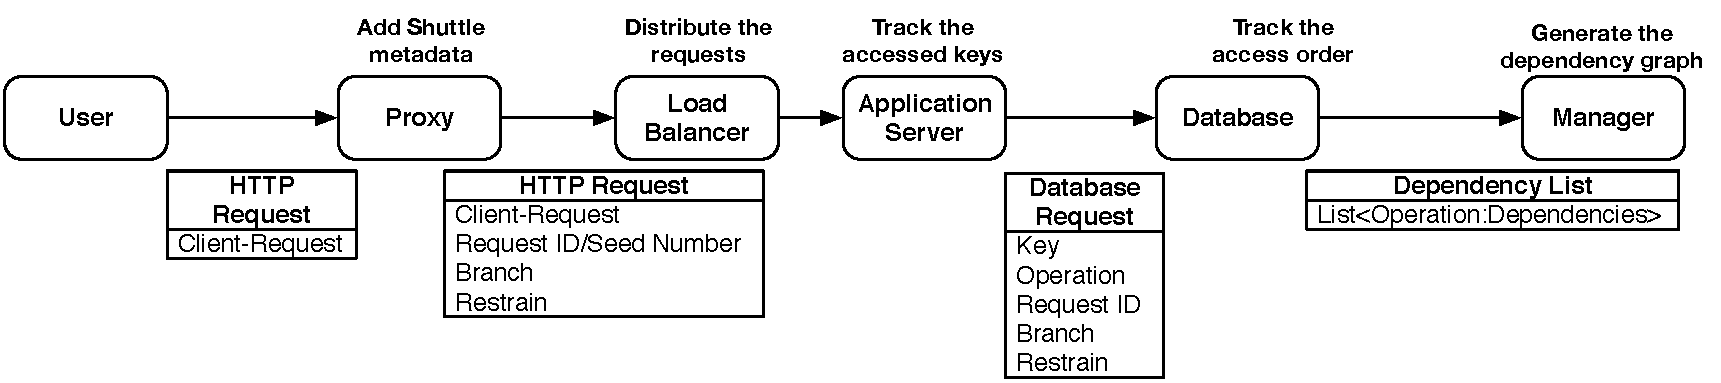
\includegraphics[width=\textwidth]{images/message_normal}
  \caption{Iterations between components during during normal execution}
  \label{fig:normal:mensaging}
\end{figure}



%%%%%%%%%%%%%%%%%%%%%%%%%%%%%%%%%%%%%%%%%%%%%%%%%%%%%%%%%%%%%%%%%%%%%%%%%%%%%%%%%%%%%%%%%%%%%%%%%%%%%%%%%%%%%%%%%%%%%%%%%%%%%
\subsection{Proxy}\label{sec:impl:normal:proxy}
The proxy retrieves all \ac{HTTP} user requests and adds the \acf{SRD} to their headers. The \ac{SRD} contains the following fields:
\begin{enumerate}
	\item \acf{RID}.
	\item Branch: the branch accessed by the request.
	\item Restraint: to support branch change during the recovery phase.
\end{enumerate}

The proxy could be implemented using a current proxy implementation, e.g. HAProxy or Nginx. Their implementations are well tested in production and are implemented in C. They are likely to perform better than a prototype using a higher-level language, such as Java (Section \ref{sec:eval:performance:proxy}). However, for sake of suppose simplicity, we implemented a new \ac{HTTP} proxy using Java. Nevertheless, implementing most part of the \ac{HTTP} specification in an efficient manner using Java ended up to be a complex task.


\begin{figure}
  \centering
  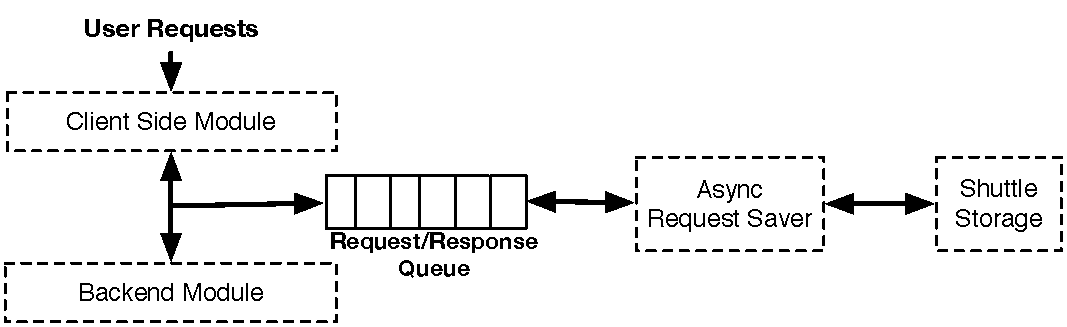
\includegraphics[width=0.7\textwidth]{arch/proxy}
  \caption{Proxy internal modules}
  \label{fig:impl:proxy_modules}
\end{figure}

The proxy is made of three parts: the client-side module, the backend module and the asynchronous request saver (Figure \ref{fig:impl:proxy_modules}).

The client side module retrieves the \ac{HTTP} requests, parses their content and modifies their headers. We used the \acf{NIO} library of Java to implement a TCP server. The server retrieves user requests and modifies their header (Algorithm \ref{code:proxy_service}). The Shuttle state is stored in the proxy but defined by the manager: \emph{branch}, \emph{restrain} and \emph{replay}. The \acf{RID} is a timestamp. Java provides timestamps with a precision of millisecond. This precision limits the proxy performance to one thousand requests per second. Therefore, we used a counter to identify the same millisecond, up to 1000 requests per millisecond (1 million requests per second). The precision of the timestamp weights on the network and storage overhead. The \ac{RID} is also used as a timestamp for the application and as a pseudorandom number generator, so the request generates always the same sequence of non-repeating numbers. The fields of \acf{SRD} represent a fixed overhead of 35 ASCII characters, corresponding to 35 bytes, in every request header.

Proxy's TCP client threads send the requests to the load balancer. We use a fixed size thread pool to associate each \ac{HTTP} response to the correct \ac{HTTP} request. The thread that retrieves, processes and forwards the request to the load balancer, blocks until its response is retrieved. A future work shall implement the proxy as a fully asynchronous proxy. To do so, the application server shall include the \ac{SRD} in the responses. Since the delay of creating a new TCP connection to the load balancer is considerable, our implementation keeps the TCP session with the load balancer and implements the \ac{HTTP} keep-alive specification. \ac{HTTP} keep-alive is a standard that allows a single TCP connection to send and receive multiple \ac{HTTP} requests/responses, instead of opening a new connection for every request/response pair. 

\begin{algorithm}
	\DontPrintSemicolon\SetKwProg{fn}{Function}{}{}
		\KwIn{received user \ac{HTTP} request}
		\KwResult{user \ac{HTTP} request with modified header}
		\SetKw{KwInit}{Initialization:}\KwInit{establish a \ac{HTTP} connection to the load-balancer}\;
		\BlankLine 
		\Letv{package}{Read TCP package from client}\;
		\Letv{request}{Parse $package$ to bound \ac{HTTP} request}\;
		\Letv{SRD}{Get Shuttle's state: $id, branch, restrain$}\; 
		Add $SRD$ fields to request's header formated as: \newline ID: $id$ \newline B: $branch$ \newline R: $restrain$\;
		Send $request$ to load balancer\;
		Add $SRD$ and $request$ to $queue$\;
		\tcc{Retrieve response}
		\Letv{package} {Read TCP package from load balancer}\;
		\Letv{response} {Parse $package$ to bound \ac{HTTP} response}\;
		\Letv{endTimestamp} {get current system time}\;
		Send $response$ to client\;
		Add $endTimestamp$ and $response$ to $queue$\;
  	\caption{Proxy}
	\label{code:proxy_service}
\end{algorithm}



%how to store the data?
Shuttle proxy stores $requests$, $responses$, $endTimestamps$ and $SRD$ in the Shuttle storage. If the data would be sent synchronously to the storage, then the response delay would increase. Therefore, we implemented a message queue (Figure \ref{fig:impl:proxy_modules}). The client-side and backend module add the data as a message in the queue. Worker threads dequeue the messages and store the data in Cassandra. This allows asynchronous behavior: requests can proceed before the transmission has finished. The worker threads are wake when the queue reaches a defined threshold or a timeout period expires. The message queue is implemented as a \emph{synchronized list} in Java.


 %%%%%%%%%%%%%%%%%%%%%%%%%%%%%%%%%%%%%%%%%%%%%%%%%%%%%%%%%%%%%%%%%%%%%%%%%%%%%%%%%%%%%%%%%%%%%%%%%%%%%%%%%%%%%%%%%%%%%%%%%%%%%
\subsection{Application Server}\label{sec:impl:normal:compute}
%Goals
The Shuttle implementation in application servers shall meet two architecture requirements: log the database accesses per request and include the requests' \ac{SRD} on every database invocation. We want to limit the number of hooks in the application and avoid modifying the database \ac{API}. The database service \ac{API} shall remain equal so as the tenants applications code. Shuttle shall be transparent to application developers.\\


%how to pass the ID?
Shuttle architecture establishes that every database operation must include the \acf{SRD}. To do so, we could implement a proxy that modifies every database request or modify the database client \ac{API} to include the \ac{SRD} as an argument. For sake of performance, we modified the Voldemort client to include the \ac{SRD} field on every database operation. We modified the Voldemort messages, which are described using \acf{protobuf} \acs{IDL} (Appendix \ref{appendix:voldemort_api}). The implemented \emph{interceptor} gets the \ac{SRD}, which is written in request header, tracks the access and invokes the modified Voldemort client (Algorithm \ref{code:database_client_interceptor}).

\begin{algorithm}
\DontPrintSemicolon\SetKwProg{fn}{Function}{}{}
\SetKwFunction{Put}{put}\SetKwFunction{VPut}{voldemort.put}\SetKwFunction{AddKey}{trackAccess}
 
 \fn{\Put{key, value, store}}{
  \Letv{srd}{\AddKey(key, store, "put")} \tcp*{get SRD and track access(Algo.\ref{code:interceptor_code_access})}
  \VPut{key, value, srd}\;
  }{}
\caption{Voldemort \ac{API} interceptor (example of put operation)}\label{code:database_client_interceptor}
\end{algorithm}

In order to extract the \ac{SRD} from the requests' header, we took in account that \ac{PaaS} systems deploy applications in application engines. In concrete, AppScale deploys the Java applications on the servlet engine WildFly \cite{wildfly} (formerly known as JBoss). In addition, most of Web Service frameworks, e.g. \ac{JAX-WS}, and \acf{MVC} frameworks, such as Spring, encompass the concept of interceptor chain, also known as filters or handlers. An interceptor chain is a sequence of handlers that contain methods that are invoked before and after the request processing by the application controller.

We implemented an \emph{request interceptor} in Spring. Application developers only need to add a single line to their applications \emph{web.xml} file to add the developed interceptor to the interceptor chain. A future work may concern the implementation interceptor for other application engines.

We also took into account that each request in Spring is binded to a single thread. Therefore, Shuttle keeps an hash table that associates the \acf{TID} with the \acf{SRD} and list of accessed keys of the request that it is processing. The \emph{request interceptor} parses the request header and creates an entry in the hash table (Algorithm \ref{code:interceptor_code_pre}).


\begin{algorithm}
\DontPrintSemicolon\SetKwProg{fn}{Function}{}{}
\SetKwFunction{PreHandle}{preHandle}\SetKwFunction{MapPut}{map.put}
\SetKwFunction{TrackAccess}{entry.trackAccess}

	\KwData{$map$ is a static hash table}
	\KwIn{HTTP user request}
	\BlankLine
	\fn{\PreHandle{request}}{
		\Letv{keySet}{new empty list}\;
		\Letv{srd}{parse request header}\;
		\Letv{tid}{get current thread id}\;
		\Letv{entry}{create entry pair: \{$keySet, srd$\}}\;
		\MapPut{tid, entry}\;
	}{}
	\caption{Shuttle interceptor: Pre handler}
	\label{code:interceptor_code_pre}
\end{algorithm}

Before every database operation, the database client library invokes the map to log the accessed key and to resolve the current \acf{TID} to the \ac{SRD} (Algorithm \ref{code:interceptor_code_access}). The map stores associates the keys in the list associated with the current thread and returns the correct \ac{SRD}. The client library appends the \ac{SRD} in the database operation request. 

\begin{algorithm}
\DontPrintSemicolon\SetKwProg{fn}{Function}{}{}
\SetKwFunction{AddKey}{addKeyAccess}\SetKwFunction{TrackAccess}{entry.trackAccess}
\SetKwFunction{MapGet}{map.get}
	
	\fn{\AddKey{key, store name, operation type}}{
		\Letv{tid}{get current thread id}\;
		\Letv{entry}{\MapGet{tid}}\;
		\TrackAccess{key,store name, operation type}\;
		\Return{$entry.srd$}
	}{}
\caption{Shuttle interceptor}
\label{code:interceptor_code_access}
\end{algorithm}

The post-process interceptor (Algorithm \ref{code:interceptor_code_pos}) accesses the map extracting the accessed keys and the \ac{SRD} of the current thread. The accessed keys are stored among the \ac{HTTP} request/response in the Shuttle storage. In addition, this interceptor also adds the \ac{SRD} to the response header.

\begin{algorithm}
\DontPrintSemicolon\SetKwProg{fn}{Function}{}{}
\SetKwFunction{AfterCompletion}{afterCompletion}\SetKwFunction{MapRemove}{map.remove}
\SetKwFunction{StorageAdd}{shuttleStorage.add}

	\KwData{$map$ is a static hash table}
	\KwIn{HTTP user request and \ac{HTTP} response}
	\BlankLine
	\fn{\AfterCompletion{request, response}}{
		\Letv{entry}{\MapRemove{tid}}\;
		\tcp{add accessed keys of entry to Shuttle Storage}
		\StorageAdd(srd, accessedKeys) \;
		add $srd$ to $response$ header
	}{}
	 \caption{Shuttle interceptor: After completion handler}
	\label{code:interceptor_code_pos}
\end{algorithm}



%%%%%%%%%%%%%%%%%%%%%%%%%%%%%%%%%%%%%%%%%%%%%%%%%%%%%%%%%%%%%%%%%%%%%%%%%%%%%%%%%%%%%%%%%%%%%%%%%%%%%%%%%%%%%%%%%%%%%%%%%%%%%
\subsection{Database}\label{sec:impl:normal:database}
%Goals e overview
Shuttle database proxy records database operations, selects the correct data item version to access according to the Shuttle state and performs snapshots. The proxy can be implemented in the database management system or as an external \ac{TCP} proxy that accesses the requests. In this work, we implemented proxy as a new library in the database management system. The database management system invokes the library before the execution of every database request. The proxy tracks the operations order to each data item recording an ordered list of the \ac{RID} that accessed the data item. The operation sequence of each data item is sent to the \textit{manager} to generate the dependency graph (Chapter \ref{sec:impl:normal:manager}). \\


We assume without loss of generality that applications store their state in distributed key-value stores, such as Dynamo \cite{Decandia2007}, where the values are often accessed using a \acf{CRUD} API. The simple \ac{API} reduces the performance overhead to track accesses while the independence between keys turns Shuttle into a scalable service. Shuttle can be extended to support other \acs{NoSQL} schemes, for instance column-oriented storage like Cassandra \cite{Lakshman2010a}.\\

%review/summary of Voldemort
Voldemort is a distributed database store implemented in Java. We choose in-memory and \acf{BDB} as storage engines and Protocol Buffers as serialization and message passing protocol. Voldemort provides a \acf{CRUD} \ac{API} with 3 methods: get, put and delete. Voldemort accepts asynchronous concurrent writes and treats the result of each modification as a new and immutable version of the data. It detects versions conflicts at read-time and handles them using vector clocks or semantic reconciliation. In this implementation, we assume the replication mechanisms to be disabled. 

%Client side (review)
In previous section (Section \ref{sec:impl:normal:compute}), we introduced the modified version the Voldemort client library, which encompasses the Shuttle interceptor. The interceptor adds the requests' \ac{SRD} to every database operation. We modified format of the Voldemort messages, which are described using \acf{protobuf} \acs{IDL}, to encompass the \ac{SRD} (Appendix \ref{appendix:voldemort_api}). This technique makes Shuttle transparent for application developers.\\


%server side: general architecture
The Voldemort implementation has been modified to invoke the Shuttle database proxy on every \ac{API} call. The proxy architecture is based on the strategy design pattern: two operation schedulers decide how the operations shall be processed. The first scheduler is used by  operations of new incoming requests, named \emph{newScheduler}, the second, \emph{replayScheduler}, described in Section \ref{sec:impl:recovery:database}, is used by operations of requests being replayed (Figure \ref{fig:scheduler_uml}). Schedulers control the access to data items ordering the operations execution and selecting the correct version of data item to access, i.e., the snapshot and branch of the data item to be read/written by the operation. Voldemort is a key-value store, i.e., each data item is identified by an unique key. We implement the versioned storage concatenating the key with the version's snapshot (a version/snapshot can only be written in one branch).

\begin{figure}
  \centering
  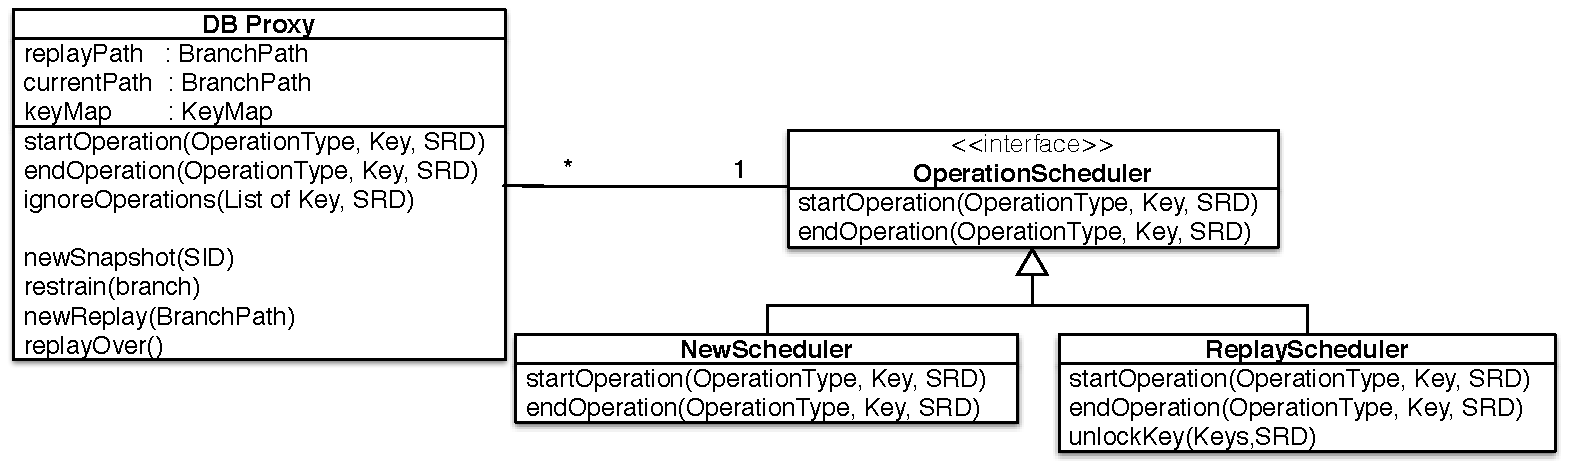
\includegraphics[width=\textwidth]{arch/scheduler_uml}
  \caption{UML of Database proxy and schedulers}
  \label{fig:scheduler_uml}
\end{figure}

%How to distinguish between new requests and replay requests? The replay flag can be removed
Each database proxy maintains two \emph{BranchPath}. A BranchPath of a certain branch is the sequence of non-tampered snapshots between the current snapshot and the root snapshot (Chapter \ref{sec:arch:runtime_recovery}). The first BranchPath, named \textit{current branch}, refers to the branch used by new incoming requests, while the second, named \textit{replay branch}, wraps the branch used by the requests being replayed.

Before each replay process, the Shuttle manager sends the BranchPath of the new branch, in which the requests will be replayed. At the end of replay process, the database nodes are also notified and the \textit{replay branch} becomes the \textit{current branch}. If the request branch is the \textit{replay branch}, then the request is a request being replayed. Otherwise, its a new request.\\


%New operations
First, we consider operations of new incoming requests. Shuttle tracks operations of new requests and allows a single write or multiple read per key. To do so, the Shuttle interceptor invokes the \emph{newScheduler}, which invokes the \emph{keyMap} (Figure \ref{fig:sequence_normal}). The \emph{keyMap}, which is the main data structure of database proxy, is a concurrent hash table that binds each  key to its Shuttle metadata, named \emph{keyMapEntry}. To improve Shuttle's performance, the \emph{keyMap} is internally partitioned to permit concurrent reads and updates.

\begin{figure}
  \centering
  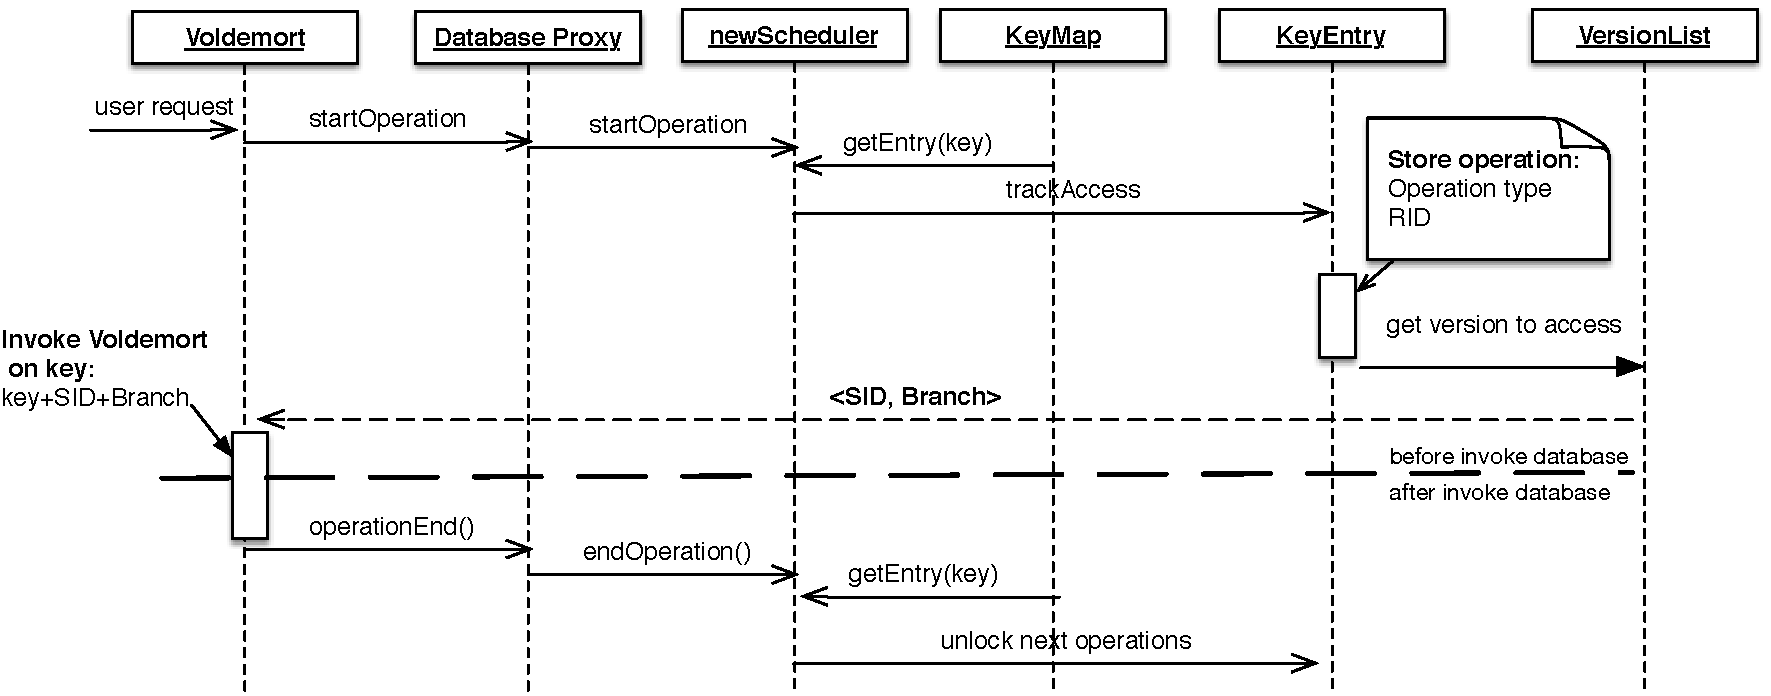
\includegraphics[width=\textwidth]{arch/operation_database}
  \caption{Sequence of invocations between the main data structures of database proxy }
  \label{fig:sequence_normal}
\end{figure}


Each \emph{keyMapEntry} object wraps the Shuttle metadata for one key/data-item: \emph{version list}, \emph{operation list} and \emph{read-write lock} (Figure \ref{fig:keymap}). The \emph{version list} contains the list of versions (snapshot-branch) in which the entry as been written because the data item may not be written in every snapshot (Section \ref{sec:arch:runtime_recovery}). 

\begin{figure}
  \centering
  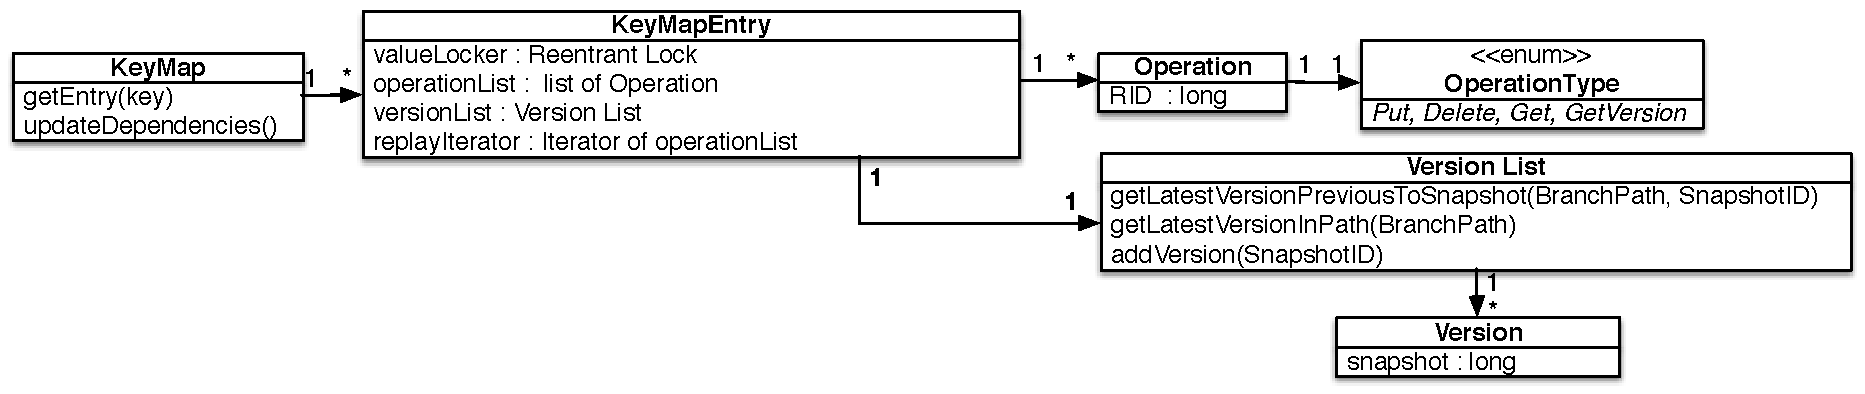
\includegraphics[width=\textwidth]{arch/keymap}
  \caption{KeyMap UML: the entities used to to track operations and versions of each key.}
  \label{fig:keymap}
\end{figure}


The \emph{operation list} contains the sequence of operations of a certain key (data item). Each operation has an operationType (put, get, delete, get version) and the \ac{RID} of the retrieved requests. The \emph{read-write lock} lock serializes the operation that access the key value allowing concurrent reads or a single write at each time. This pessimistic concurrency control method may decrease the system performance comparing, for instance, with a multi-version concurrency control. An alternative implementation can write the \ac{RID} among the value in the store and track only the read accesses, parsing the accessed \ac{RID}. The client-library may parse the value to get the \ac{RID} but the write order is relevant. For sake of simplicity, we used a pessimistic concurrency control with a reentrant mutual exclusion lock.\\

%Read/Write lock, add operation and get the correct version
When \emph{newScheduler} is invoked by an operation from a new incoming request, it gets the \emph{keyMapEntry} of the key and attempts to gain the access to its \emph{read-write lock} (Algorithm \ref{code:snapshotAlgorithm}). Then, it adds the operation to the \emph{operation list}. At last, Shuttle gets the correct version to access based on the \emph{BranchPath} and the \emph{list of versions} of the key (Section \ref{sec:arch:runtime_recovery}). 

If the request \ac{RID} is smaller than the current \acf{SID} (line \ref{line:snapshot:1}), then the request does not belong to the current snapshot and shall access the latest, but previous to the snapshot instant, version of the value that is in the  \textit{current BranchPath}. Otherwise, the request belongs to the current snapshot. Read operations access the latest version (line \ref{line:snapshot:2}) in the  \textit{current BranchPath}. A write request may create a new version if the version has yet not been written in the current snapshot (\ac{RID} is bigger than the \ac{SID} of the latest version) (line \ref{line:snapshot:3}). Versions are created with the current \acf{SID}. The key accessed by the request is the concatenation of the original key with the snapshot(version) returned by the Algorithm \ref{code:snapshotAlgorithm}. After the access, the \emph{read-write lock} is unlocked and the next operations proceed. We implement copy on write by creating a new key version when required. \hl{isto é talvez o mais complexo e fundamental de toda a tese, tem de ficar perceptivel}


\begin{algorithm}
\DontPrintSemicolon\SetKwProg{fn}{Function}{}{}
\SetKwFunction{TrackAccess}{trackAccess}\SetKwFunction{AddOperation}{operationList.add}
\SetKwFunction{WriteLock}{lock.writeLock}\SetKwFunction{ReadLock}{lock.readLock}
\SetKwFunction{AddVersion}{versionList.add}

	% \KwData{$map$ is a static hash table}
	% \KwIn{HTTP user request and \ac{HTTP} response}
	\BlankLine
	\fn{\TrackAccess{operation type, srd, branchPath}}{
		\eIf{type is put or delete}{
			\WriteLock{}\;
		}{
			\ReadLock{}\;
		}
		\BlankLine
		\AddOperation{new Operation(type, srd.rid)}\;
		\BlankLine
		\eIf{srd.rid < branchPath.sid}{  \label{line:snapshot:1}
			\tcp{Access only the versions of previous snapshots}
			\Return latest version in $(version list \cap branchPath : version < srd.rid)$\;
		}{
			\tcp{Access the latest version}
			\Letv{latest}{get latest version in $(version list \cap branchPath)$}\;
			\If{type is get}{
				\Return	 $latest$\; \label{line:snapshot:2}
			}
			\tcp{New version is created if the request belongs to a newer snapshot}
			\If{branchPath.sid > latest.sid}{ \label{line:snapshot:3}
				\Letv{version}{new Version(branchPath.sid)}\; 
				\AddVersion{version}\;
				\Return{version}\;
			}
		}
	}{}
	 \caption{Method to track a new request, get the version to access and perform snapshot}
	\label{code:snapshotAlgorithm}
\end{algorithm}

Since the \emph{version list} keeps a pointer to the latest version and the pointer is updated if wrong, the average complexity of the Algorithm \ref{code:snapshotAlgorithm} is \O{1}: get the latest version and check if it belongs to the BranchPath, which is a HashSet. If the BranchPath size becomes a considerable storage overhead, the BranchPaths and version lists can be implemented as a bitmaps.

\begin{figure}
  \centering
  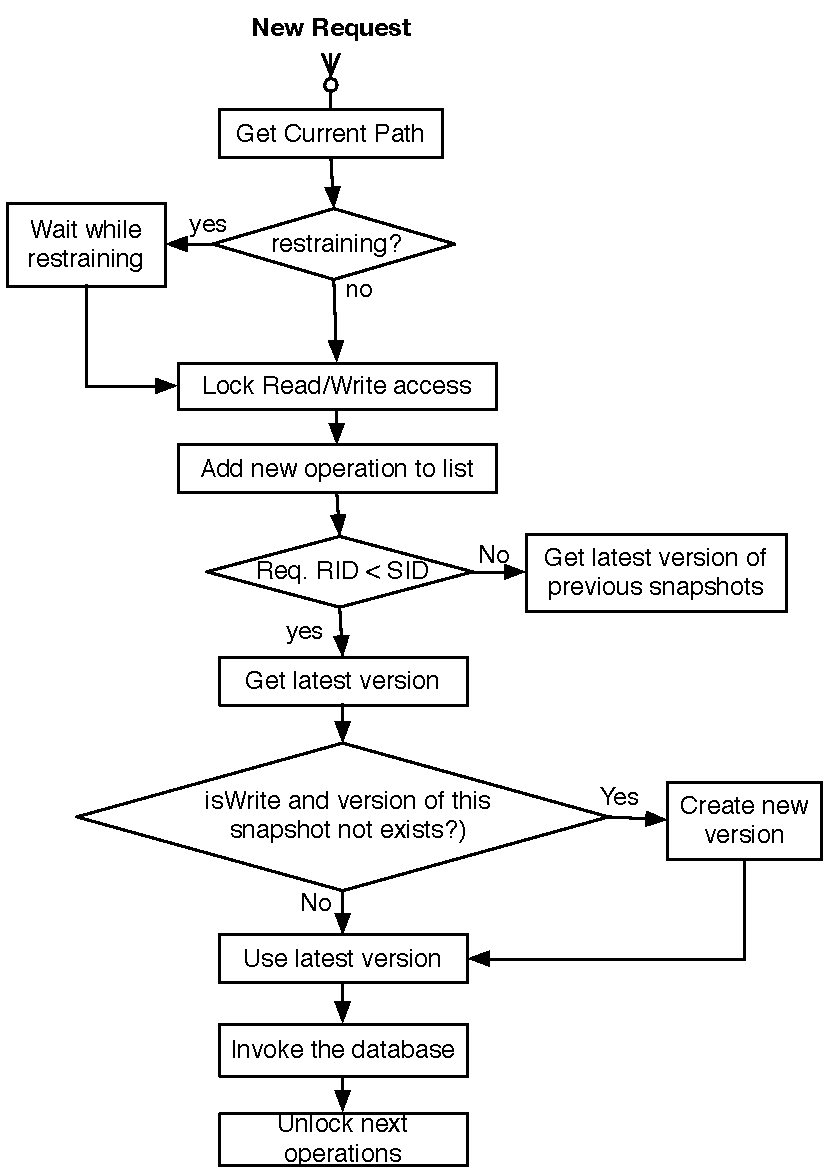
\includegraphics[width=80mm]{arch/database_proxy_logics}
  \caption{Diagram of processing a new database request}
  \label{fig:impl:database:process_new}
\end{figure}
	
%collect dependencies
Shuttle collects the dependencies between requests transversing the operation list of every \emph{KeyMapEntry} in the \emph{KeyMap}. Each \emph{KeyMapEntry} keeps a pointer to the latest collected dependency in the operation list, so only new operations are transversed.

Algorithm \ref{code:dependency_collection} firstly lookup for the write operation previous to the latest collected operation. Then, it iterates the operations following to the latest collected operation. If an operation of request $A$ reads a data item written by an operation of request $B$, then $A$ depends from $B$. Dependencies are logged on a hash table that associates the operation \ac{RID} with the \ac{RID}s which it depends from. Every database node sends its $dependenciesTable$s to the manager periodically. 

 
\begin{algorithm}[H]
\DontPrintSemicolon\SetKwProg{fn}{Function}{}{}
\SetKwFunction{Add}{dependencies.add}
	\SetKw{KwInit}{Initialization:}\KwInit{\Letv{dependencies}{new hash table<Long,Long>}}\;
	\BlankLine
	\ForEach{$entry$ in $keyMap$}{ 
		\Letv{lastWrite}{\ac{RID} of the latest write operation previous to the earlier operation to collect}\;
		\ForEach{operation \textbf{in} entry.operationList}{
			\eIf{operation.type == READ}{
				\Add{operation.rid, lastWrite}\;
			}{
				\Letv{lastWrite}{operation.rid}\;
			}
		}
		\Letv{entry.lastCollected}{latest operation in $entry.operationList$}\;
	}
	\BlankLine
	send $dependenciesMap$ to manager\;

 \caption{Dependency collection}
\label{code:dependency_collection}
\end{algorithm}


%Scalability
\acs{NoSQL} databases are designed for distributed environments. The proposed dependency tracking and snapshot mechanisms are horizontally scalable: each database node remains independent and each data item is independent from the others. The only locks shared by a sub-set of data items are the KeyMap partition lock and the KeyMapEntry lock. Adding more partitions, can improve the overall performance. Each node is responsible for logging local dependencies and communicates to a central entity (Manager) to update the  dependency graph. 


\subsection{Manager}\label{sec:impl:normal:manager}
%summary
The manager retrieves dependencies, orders to create new database snapshots and coordinates the recovery process. 

%When and how retrieves
The manager aims to retrieve database operations and generate the dependency graph. Dependencies are pushed to the manager by the database nodes. The dependency graph is updated during the normal execution. An alternative approach could pull the dependencies from each database node during the recovery phase and generate the graph during the recovery period.

%Definition
The dependency graph is a set of vertices, each one representing a request, and a collection of edges that each connect a pair of vertices. Each edge specifies an one-way dependency between two requests. Therefore, the dependency graph is a directed graph. The dependency graph is also \emph{not connected}, i.e., it consists of a set of connected subgraphs. Each vertex is uniquely identified by its key, the \ac{RID} of the request that it represents. 


The dependency graph has 4 main operations: insert new dependencies, get requests sorted by start instant, get requests dependent from a certain request, get requests from which a certain request depends from.

The first operation inserts new vertexes (requests) and adds edges between the new vertexes and all the vertex from which the new vertexes depends from. The second visits every vertex by the order of their key (start instant). The two latest operations visit all vertexes reachable from a certain vertex using the \emph{dependencies to} and the \emph{dependencies from} directions, respectively. Even the dependency graph is, conceptually, a directed graph, the two latest operations are easier to implement on \emph{undirected graphs}.

Two of the main representations of graphs are: adjacent matrix and adjacent list. On a dependency graph, each insert operation requires to create several edges, one per dependency. An edge can be inserted on an adjacency matrix with complexity \O{1}. However, we consider the dependency graph to be a \emph{sparse graph} because each request is expected to be dependent from a small part of the remaining requests. Therefore, the adjacent list representation is expected to be more space efficient than the matrix.

The three main implementations of a adjacent list graph are: an indexed array, object oriented and a hash table. The vertex keys are expected to be a sparse numeric sequence with irregular number of edges. Therefore an indexed array implementation would not be space efficient. Insert operations in object oriented graphs requires searching for objects to create new edges. However, a graph search algorithm, for instance breadth-first search (BFS), has a time complexity of \O{|Vertix|+|Edges|} in the worst case.
Hash table implementations use a hash table to associate each vertex in a graph with an array of adjacent vertices. To clarify, each hash table object represents a vertex. The object has list of keys that represents the edges. \\

We implemented the dependency graph as a hash table. Doing so, insert operations have \O{1} complexity. Operations to obtain the first level of dependencies of a certain requests has also have \O{1} complexity. Even so, we also take in consideration that the performance of these operations is influenced by constant factors and by the hashing function and data distribution.

The hash table keys are the \acf{RID}, which is also the start timestamp of the request. The object associated with each key wraps: the end timestamp; the list of requests from which the request depends from (executed before); the list of requests dependent from the request (to execute after)(Figure \ref{fig:impl:manager:graph}). For sake of simplicity, the graph is kept in the memory of the manager. A production mode implementation, in which the memory limit can become a bottleneck, shall implement the dependency graph in a \acf{DHT} or a key-value \acs{NoSQL} store.


\begin{figure}
  \centering
  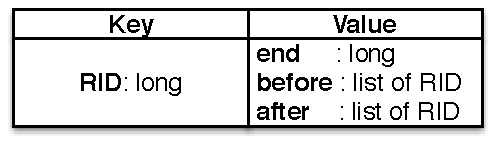
\includegraphics[width=50mm]{arch/managerGraph}
  \caption{Entry of the dependency graph HashMap}
  \label{fig:impl:manager:graph}
\end{figure}


%how it stores the dependencies
The manager updates the dependency graph when a new table of dependencies is retrieved from a database node (Algorithm \ref{code:add_dependency_graph}). The retrieved hash table associates each \acf{RID} with the \ac{RID} of the requests from which the request depends from. The algorithm creates two graphs: the first representing the dependencies from; the seconds the dependencies two. In other words, the graphs are symmetric: one graph can be generated inverting the directions of the edges of the other graph.

 \begin{algorithm}[H]
 \DontPrintSemicolon\SetKwProg{fn}{Function}{}{}
 \SetKwFunction{Add}{entry.addBefore}\SetKwFunction{AddAfter}{entry.addAfter}
 	\KwIn{\Letv{dependencies}{HashTable<RID, list of RID>}}\;
 	\BlankLine
 	\ForEach{$\{rid, dependencyList\}$ in $dependencies$}{
 		\Letv{entry}{get or create a GraphEntry in dependency graph for $rid$}\;
 		\Add{$dependencyList$}\;
 		\BlankLine
 		\ForEach{$dependentRID$ in $dependencyList$}{
	 		\Letv{entry}{get or create a GraphEntry in dependency graph for $dependentRID$}\;
	 		\AddAfter{rid}\;
 		}
 	}
 	\caption{Add dependency to dependency graph}
	\label{code:add_dependency_graph}
\end{algorithm}

%Branching
The manager maintains the \textit{BranchTree}. BranchTree is the implementation of the branching model introduced in Chapter \ref{sec:arch:runtime_recovery}. The BranchTree is implemented as a hash table that associates each branch and its snapshots. The tree model allows tenants to create new branches or snapshots.

In order to create a snapshot, tenants define a future instant in time, $t$, when the snapshot will occur. The manager forwards the value of $t$, named \acf{SID}, to every database instance. Each database node adds a new snapshot with the retrieved \ac{SID} in the \emph{current branchPath}. The manager insert the \ac{SID} in the entry of the current branch in the \emph{BranchTree}.

In order to create a new branch and start a new replay process, tenants shall specify a base snapshot. The branching algorithm finds the branch of the selected snapshot and copies the snapshots in the list, which are equal or previous to the selected snapshot, to create a new entry in the BranchTree for the new branch. Then, the algorithm creates a snapshot in the new branch. In other words, the new BranchPath is the concatenation of the new snapshot, in which the replay will be written, and the sequence of snapshots of the branch of the selected snapshots that are equal or previous to it. The new BranchPath is send to the database proxy of all database nodes.\\


%Communication
Shuttle's manager prototype retrieves tenants commands via command line. Each module of Shuttle, including the manager, has a TCP server that retrieves requests from other modules. Requests are formatted using Google's Protocol Buffer \cite{protobuffers}. Messages exchanged between the manager and the remaining modules are in Appendix \ref{appendix:shuttle_api}. \hl{vale a pena extender?}



\section{Recovery}\label{sec:impl:recovery}
%overview
In this section, we introduce the implementation of the recovery process in Shuttle.\\

The recovery process begins when the tenant selects a non-tampered snapshot. The manager creates a new branch and sends its \emph{BranchPath} to all database proxies. The proxies set the new BranchPath as \emph{replay branch} (Chapter \ref{sec:impl:normal:database}). After, the manager generates the sequence of requests to replay, named \emph{execution list}. The replay instances are allocated and retrieve this list (Figure \ref{fig:messaging_replay}). Then, the replay instances are notified to start replaying the requests. After replaying all the requests, each replay instance notifies the manager. The manager sets the proxy state to \emph{restraining mode} and commands the replay instances to replay the incoming requests retrieved during the recovery period. After replaying the remaining requests, the database nodes are notified to disable the restrain and \emph{replay branch} becomes the \emph{current branch}. At end, the proxy \emph{restraining mode} is disabled and the following new requests are done in the new branch.

\begin{figure}
  \centering
  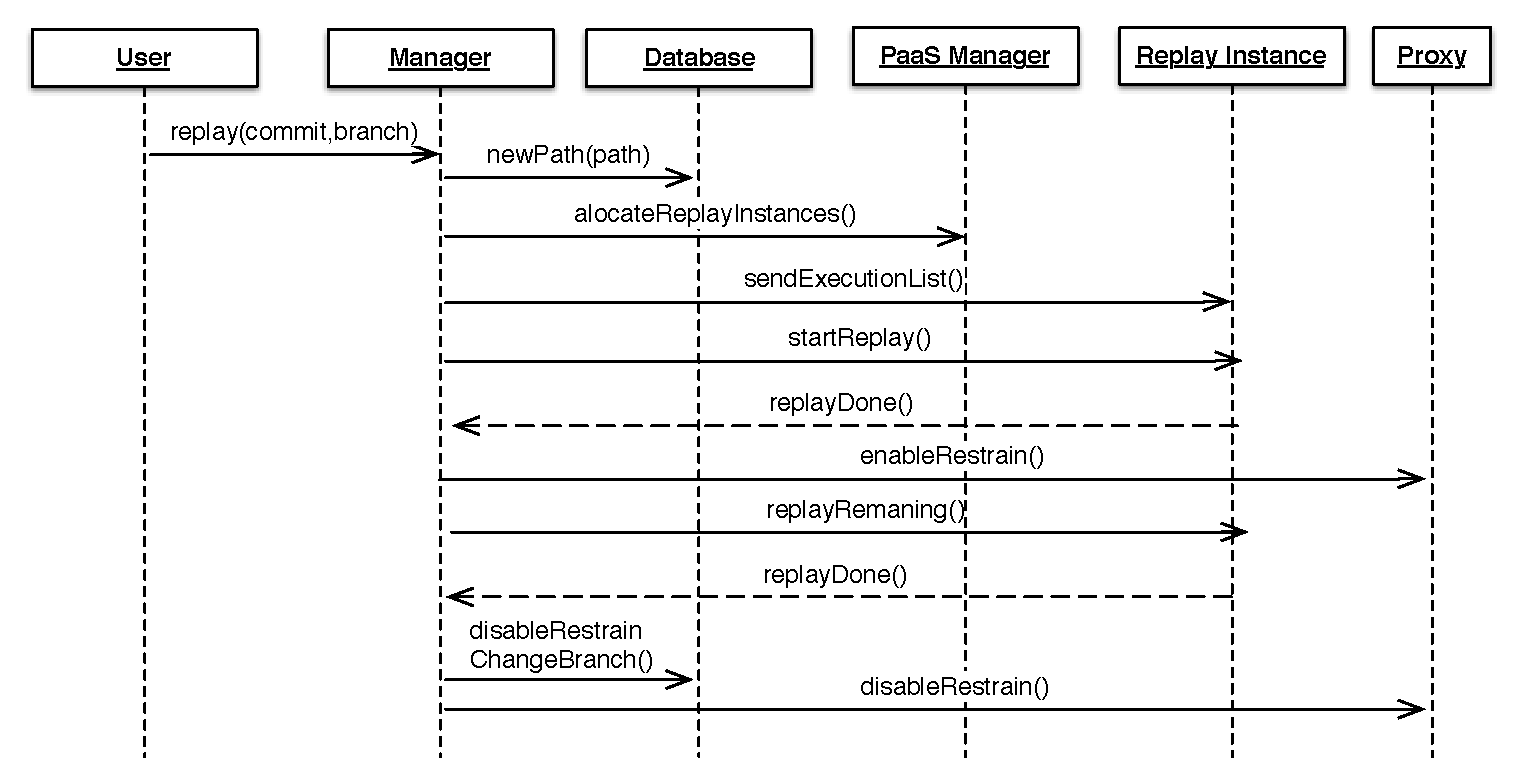
\includegraphics[width=140mm]{images/message_replay}
  \caption{Message sequence during replay phase}
  \label{fig:messaging_replay}
\end{figure}


\subsection{Manager}\label{sec:impl:recovery:manager}
Tenants, selecting a snapshot that does not contain the result of any malicious action, start the recovery process. Shuttle creates a new branch and sends its \emph{BranchPath} every database proxy. After, the manager generates the request execution list, i.e., the sequence by the requests shall be replayed.

Shuttle can perform selective or full replay. It also can use clustering to re-execute different sequences of requests in parallel or not (Table \ref{tab:operation_types}).

%full-replay
Shuttle uses the Algorithm \ref{code:start_end_full_replay} to generate a request execution list for full-replay. The algorithm implements the start-end request ordering approach proposed in Section \ref{sec:arch:dependencies}. Since the graph is implemented as a hash table (Section \ref{sec:impl:normal:manager}), the keys are not ordered. At recovery time, the keys are ordered and the graph is iterated in order. The complexity of this operation is \O{n \log{} n}. A request must be executed concurrently with a previous request if it began before a previous request ends. Otherwise, the request was not executed concurrently with any of the previous requests.

\begin{algorithm}[H]
\DontPrintSemicolon\SetKwProg{fn}{Function}{}{}
\SetKwFunction{Max}{max}
	  \KwIn{$graph$: dependency graph (Hash Table)}
	  \KwIn{$snapshot$: non-tampered \acf{SID} selected by the tenant }
	  \KwOut{$executionList$: sorted list of \ac{RID} to replay}
	  \BlankLine
	  Sort $graph$ keys\;
	  \BlankLine
	  \Letv{latestExecuting}{-1}\tcp*{the biggest end timestamp being executed}
	  \ForEach{$request$ in $graph$}{
	      \eIf{$request.start => latestExecuting$}{
	      	  
	          add $separator$ to $executionList$ \tcc{none of following requests were executed concurrently with previous}
	      }{
	          add $request$ to $executionList$\;
	      }
	      \Letv{latestExecuting}{\Max{latestExecuting,request.end}}\;
	  }
	\caption{Start-end ordering algorithm}
	\label{code:start_end_full_replay}
\end{algorithm}


%clustering
The clustering mechanism identifies the connected subgraphs of the dependency graph. The algorithm traverses the vertex marking all nodes adjacent that are reachable from a node. The set of nodes reachable from a node, defines a cluster. Then, we choose a non-marked node and repeat the procedure.\\

%selective-replay
When the tenants provide a set of malicious actions, $A_{intrusion}$, Shuttle performs selective replay instead of replaying every request. The selective replay uses the dependencies between requests to expand a provided set of malicious requests, $A_{intrusion}$,  to get which requests are needed to be replayed. Set of malicious requests is expanded adding all requests dependent from the initial malicious request set. The traversed nodes are the tainted requests, $A_{tainted}$. Then, the set $A_{tainted}$ is expanded transversing the nodes of the set on the opposite direction: visit requests from which the traversed node depends from and that are posterior to the selected snapshot (Figure \ref{fig:selectiveGraph}). The list of data items read by the requests in $A_{replay}$ is obtained querying the Shuttle storage. The storage contains the keys accessed per request, which was logged by the application servers (Section \ref{sec:impl:normal:compute}). The snapshot versions of these items is loaded and the requests in $A_{replay}$ are replayed. The modified data items are merged with the current database data without: the \emph{branchPath} of a selective replay branch wraps the current \emph{branchPath}. This mechanism avoids tainting the modified data items and copying them into the current database state. This mechanism does not support runtime recovery but the recovery period is considerably smaller than using full-replay. \hl{figura para ajudar? codigo? ou está bem perceptivel?} \\

%\item \textit{If a replayed request operation a different entry, then the requests which access the entry are also replayed.}
%During the replay phase, requests may access different data items than the ones during the first execution. If the value of the data item is not-updated because non of the tainted requests accessed the entry before, then, every request that access the entry is also tainted and replayed before the current access proceed.
%After each replayed request, the performed database operations are compared with the original set of operations. For each key of the operations performed originally but not in the replay, are unlocked. For each key of the operations performed on replay but not originally, the following operations are also replayed. 


\subsection{Replay Instances}\label{sec:impl:recovery:replay}

%How they can work?
The Shuttle manager requires the \ac{PaaS} controller to launch a set of \textit{replay instances}. If the \ac{PaaS} system does not support auto-scaling, the manager can request the \ac{PaaS} controller to add new database and web-server containers to attend the flow of replayed requests. Otherwise, the auto-scaling mechanism will detect the overload of the web-servers and database and trigger the creation of new instances. In the first, the number of web-servers is changeless during the replay phase, so the instances send the requests directly to the web-server instances, avoiding the overhead of load-balancer. In the later, the requests are sent to the load-balancer that distributes the requests through the instances. In current implementation, requests are sent to the load-balancer because AppScale supports auto-scalling and the number of instances during the replay phase is unknown.\\

%How they they are implemented to work
Each replay instance retrieves various list of \acf{RID} to execute and the branch in which they shall be executed. They have a main thread to schedule the execution and a thread pool to execute requests asynchronously. Each thread fetches the \ac{HTTP} requests from the \emph{Shuttle storage}, modifies their header setting the \ac{SRD} field \emph{branch}, sends them to the load-balancer. Each response is compared against the response during first execution. An alternative approach can compute the hash of responses in background and compare their values.

If a request has been removed, for instance if it is a malicious request, the replay instance fetches the keys accessed by the malicious request during its first execution and invokes the database proxy to unlock the execution.\\ %An alternative approach using a distributed lock per data item does not require to store the accessed keys but requires to store the replayed requests and share a lock, which can be a bottleneck. 

The prior evaluation, on serial-replay schema, showed fetching each request before sending is a considerable overhead. We duplicated the throughput and reduced the Shuttle storage usage by using a thread in background to fetch batches of requests from the Shuttle storage. The fetching thread and the execution threads communicate through a in-memory message queue.

%Flow control
The start-end algorithm (Algorithm \ref{code:start_end_full_replay}) groups the requests that shall be executed concurrently. The separator marks the end of a group of concurrent request. When a separator is reached in the request list, the execution thread waits until all responses are retrieved. Even so, the number of concurrent requests within a group can overload the servers and database instances. In addition, since application server and replay instances are supported by thread pools, the system reaches a \emph{deadlock} if all threads of one of the thread pools are blocked waiting for further requests. Taking that in consideration, all components in Shuttle shall be asynchronous and message-driven.

%Goal:
%1 - O client envia o pedido e segue o processamento do próximo
%2 - A base de dados tenta processá-lo. Se não conseguir, cria um future e prossegue.
%3 - Quem acaba e ia acordar os bloqueados, agora invoca o future para que este seja processado
%4 - A resposta é return e o client detecta o evento de nova resposta, invoka a callback e prossegue com o pedido.

%O DBProxy deveria ser semelhante a um serviço de queue e workers para que os pedidos possam ser devolvidos à queue e os workers possam continuar a processar outros pedidos. Alterantiva: usar o modelo de queue de mensagens: guardo os pedidos que tenho para processar se não derem para ser processados agora e depois, verifico se já os posso processar. volto a processá-los depois.

%A alternativa tem de ser um client baseado em callbacks. Envia o pedido, continua para outros pedidos e quando vier a resposta, associa-a ao pedido e prosseegue... problema: isto não existe em voldemort. o cassandra faz mas o voldemort não.


As requests are replayed asynchronous, the replay instances must use an end-to-end flow control protocol to avoid the sender send requests too fast for the application servers to receive and process. We implemented a simple flow control protocol, which does not have to lead with message ordering and retransmission (\ac{TCP} handles transmission failures). We established two thresholds for the number of pendent responses that define 3 steps to change the number of requests per unit of time. Consequently, the request throughput of each replay instance is dynamic to avoid the servers overload. One of main challenges to evaluate the Shuttle's prototype is to tune the threshold parameters. Future implementations shall access the \ac{PaaS} controller in order to watch the instances' metrics and do flow control based on it.\\


\subsection{Database}\label{sec:impl:recovery:database}
%how it does replay?
In Section \ref{sec:impl:normal:database}, we introduced the implementation of \emph{newScheduler}, which defines the order and logs the new operations. In this Section, we introduce the \emph{replayScheduler}, which constrains the replayed operations per data item to an order equivalent to the one during their first execution.

Database operations are processed by the replayScheduler if the \emph{branch} field of the operation \ac{SRD} is the same of \emph{replayBranch}. The replaySchedule gets the KeyMapEntry of the accessed key. Each KeyMapEntry contains the list of operations logged during the execution phase. When the first operation, which is being replayed in current replay branch, accesses the data item, Shuttle creates an operation list iterator and associates it with the key.

Operation list iterators control the replay process: it allows or blocks operations (Algorithm \ref{code:operation_iterator}). The iterator keeps a list of operations allowed, executing, waiting or to be ignored. The first allowed operation is the first operation after the snapshot selected by the tenant, i.e., the smallest \acf{RID} that matches the condition $\acf{RID} >= snapshot$ (line \ref{line:iterator:next}). If no executing and the allowed set is empty, then the iterator transverses more operations (line \ref{line:iterator:fetch}). The algorithm fetches the following consecutive read operations or one write operation. Operations previous to the selected snapshot or unlocked are ignored. If an operation is not the following operation, i.e., allowed, then the operation is delayed (line \ref{line:iterator:sleep}). The operation is removed from the \emph{executing} list after its execution and blocked operations are unlocked to check if they can access. For sake of simplicity, the concurrency control is not included in the pseudo-code. \\

\begin{algorithm}[H]
\DontPrintSemicolon\SetKwProg{fn}{Function}{}{}
\SetKwFunction{Fetch}{fetchMoreAllowedOperations}\SetKwFunction{AllowedRemove}{allowed.remove}
\SetKwFunction{Executing}{executing.add}\SetKwFunction{WaitingAdd}{waiting.add}\SetKwFunction{WaitingRemove}{waiting.remove}
\SetKwFunction{AllowedAdd}{allowed.add}\SetKwFunction{Next}{iteratorNext}\SetKwFunction{ExecutingRemove}{executing.remove}
\SetKwFunction{StartReplay}{startReplayOperation}\SetKwFunction{EndReplay}{endReplayOperation}
 	\SetKwProg{KwInit}{Initialization}{:}{}
 	\KwInit{}{
 		\Indp
	 	\textit{all}: list of all operations\;
	 	\textit{allowed}: list of operations allowed to execute \;
	 	\textit{executing}: list of operations executing \;
	 	\textit{waiting}: list of operations waiting to execute \;
	 	\textit{ignore}: set of operations to ignore \;
	 	\textit{nextOperation} $\leftarrow$ first operation after the snapshot\;
	}
 	\BlankLine
 	\BlankLine
 	\fn{\StartReplay{operation}}{
	 	\If{allowed is empty \emph{and} executing is empty} { \label{line:iterator:fetch}
	 	    \Fetch{}\;
	 	}
	 	\eIf{operation in allowed} {
	 		\tcp{move from allowed list to executing}	
	 		\AllowedRemove{operation}\;
	 	    \Executing{operation}\;
	 	}{
	 	    \WaitingAdd{operation}\;
	 	    thread sleep \tcp*{block operation} \label{line:iterator:sleep}
	 	    \WaitingRemove{operation}\;
	 	    \tcp{Attempt to execute}
	 	    \StartReplay{operation}
	 	}
	}
	\BlankLine
 	\BlankLine
 	\fn{\Fetch{}}{
 	 	\eIf{$nextOperation$ \textbf{is} write}{
 	 		\AllowedAdd{nextOperation}\;
 	 		\Letv{nextOperation}{\Next{nextOperation}} \;
 	 	}{
 	 		\tcc{add all read operations until next write}
 	 		\While{nextOperation \textbf{is not} write}{
 	 			\AllowedAdd{nextOperation}\;
 	 			\Letv{nextOperation}{\Next{nextOperation}} \;
 	 		}
 	 	}
 	}{}
 	\SetKwBlock{DoWhile}{do}{while}
 	\BlankLine
 	\BlankLine
 	\fn{\Next{operation}}{
 		\tcc{get next operation bigger than the base snapshot and not ignored}
 	 	\DoWhile{
 	 		\Letv{operation}{operation.next}\;
 	 	}\textbf{while} $operation.rid < SID$ \textit{or} $operation.rid \in ignoring$\; \label{line:iterator:next}
 	 	\Return{operation}
	}


 	\BlankLine
 	\fn{\EndReplay{op}}{
 		\ExecutingRemove{op}\;
 		\ForEach{operation \textbf{in} waiting}{
 			wake $operation$ thread\;
 		}
 	}{}
 \caption{Access iterator algorithm}
\label{code:operation_iterator}
\end{algorithm}


%unblock keys
The iterator ignores operations that belong to previous snapshot, i.e., $operation.rid < snapshot$, or to the \emph{ignoring} list. The \emph{ignoring} list contains the operations that will not be executed. If a request is malicious, the replay instances invoke the database \ac{API} method: $ignoreOperation(\ac{RID},keys)$ to ignore operations in all keys accessed by the request. 

When application servers retrieve requests and their replay flag is set, the database client library fetches the keys accessed by the requests during their first execution (Chapter \ref{sec:impl:normal:compute}). At the end of the request re-execution, the process compares the keys accessed during the replay phase against the ones accessed during the first execution. The database client library invokes the method $ignoreOperation(\ac{RID},keys)$ to ignore the operations it did not perform during the replay phase. This mechanism allows the blocked operations to proceed.

%If the request does not access all the keys than during its first execution, then the database client proxy invokes the same API. 

\hl{justifica colocar o seguinte?:} An alternative approach could be: if a request locks, then it invokes a lock, which is shared between all database servers, informing which request should execute before it and waiting. When the request ends, the lock notifies the blocked processes. This approach does not require to store the accessed keys but requires to share a lock, which can be a bottleneck, and to store which requests have been replayed. 


%runtime recovery and change branch
Shuttle supports runtime recovery, i.e., the application remains online during the recovery process (Section \ref{sec:arch:runtime_recovery}). The field \emph{branch} contained in every request allows the database proxy to separate the operations of new incoming requests from the operations of requests being replayed. The first use the \emph{current branch} while the later use the \emph{replay branch}. As introduced above, the \emph{branchPaths} and the scheduler algorithms define the versions which these operations read/write. This allows the new incoming requests to proceed during the recovery process.


At the end of the recovery process, the incoming requests must be switched to the application with fixed state, i.e., the requests should access the data items versions of the \emph{replay branch}. When all requests are replayed, the manager interact with the proxy to set the \ac{SRD} subfield \emph{restrain} in every following incoming request. The \emph{newScheduler} blocks the execution of new operations that have the \emph{restrain} flat set. Requests performed after the beginning of the replay process are replayed. After, the manager broadcasts a message to every database node to set the \emph{replay branch} as \emph{current branch} and ignore the restrain flag. The proxy is notified to stop setting the restrain flag. Consequently, the blocked requests and further new incoming requests are processed. This mechanism causes a delay on the request process in exchange for a simplicity and low communication overhead. 

%%%%%%%%%%%%%%%%%%%%%%%%%%%%%%%%%%%%%%%%%%%%%%%%%%%%%%%%%%%%%%%%%%%%%%%%%%%%%%%%%%%%%%%%%%%%%%%%%%%%%%%%%%%%%%%%%%%%%%%%%%%%%
\section{Application Example: Ask}\label{sec:impl:application}
%explain the application
We developed a \acf{QA} web application, named \emph{Ask}, to evaluate Shuttle prototype. \emph{Ask} is based on Stack Exchange \cite{stackexchange} or Yahoo! Answers \cite{yahooAnswers}. The application data structure is as follows (Figure \ref{fig:DataStructure}). A question has a title, a known number of views by clients, a set of tags, which represent the themes of the question, and a set of answers. Each answer has a text and a number of user votes. Each user can only do a single vote per answer, incrementing or decrementing one unit the number of votes. Each answer has a set of comments.

 \begin{figure}
   \centering
   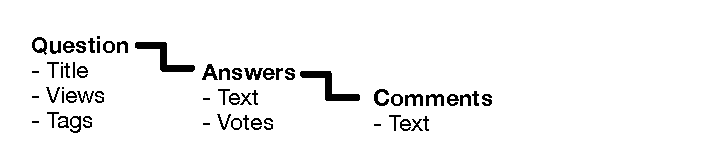
\includegraphics{images/questionStructure}
   \caption{Data structure}
   \label{fig:DataStructure}
 \end{figure}

The data is stored in four Voldemort stores: questions, answers, comments and tags. For example, insert a new answer requires to add an entry to the \textit{answers store} and modify the entry of the corresponding question in \textit{questions store} to update the answer list. 
Independent user sessions would be trivial to replay in parallel. The application semantics implies the following dependencies: a) questions are independent; b) a new answer depends from previous answers and votes to the same question; c) a new comment depends from the commented answer; d) a new vote depends from the voted answer (Table \ref{tab:dependencyTable}). In Chapter \ref{sec:eval:accuracy}, we compare the number of clusters considering or not dependencies between questions with the same tag.
\begin{table}
  \centering
   \begin{tabular}{|l|l|l|l|}
    \hline
    ~             & Read           	& Write           	& Depend from                               \\ \hline
    New Question  & (Tags)          & (Tags) Question  & (Tags)                                     \\ \hline
    New Answer    & Question        & Question, Answer & Previous answer to the same question   \\ \hline
    New Comment   & Answer          & Answer, Comment  & Commented answer                           \\ \hline
    New Vote      & Answer          & Answer, Vote     & Voted answer                               \\ \hline
    \end{tabular}
    \caption{Dependency list}
    \label{tab:dependencyTable}
\end{table}

Figure \ref{fig:dependencyGraph} represents the application dependencies graph generated by Shuttle when two questions, two answers and one comment are created. Questions are independent, since they don't share a tag. Dashed entries represent read-only requests without consequent writes. A future work may consider to ignore these requests.

\begin{figure}
  \centering
  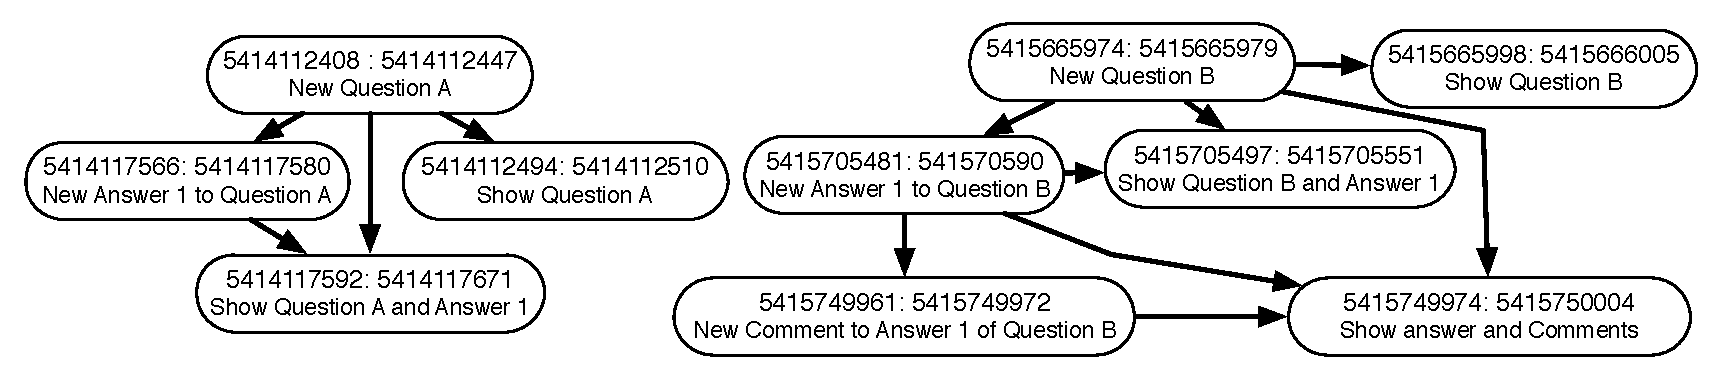
\includegraphics[width=150mm]{images/dependencyGraph}
  \caption{Example of a dependency graph generated by Shuttle}
  \label{fig:dependencyGraph}
\end{figure}

The application is implemented using Java Spring \cite{spring}, which is one of the most used Java enterprise web systems and it is compatible with most of the current \ac{PaaS} systems (Section \ref{sec:impl:adopted_technologies}). The implementation is independent of Shuttle. Shuttle does not require the application to be modified, except adding the Spring interceptor (Section \ref{sec:impl:normal:compute}). 


In order to use real-world data, we selected subsets of a dump of the Stack Exchange database \cite{stackexchange_data}. StackExchange is ranked 57th for traffic in the world \cite{websiteRanking}. A 24 hours window has: 36 million page loads, 148 million \ac{HTTP} requests (1712 requests per second), 267GB retrieved, 1TB sent, 334 million \ac{SQL} queries \cite{stackStatistics}. A question takes, in average, 28ms to be rendered. The architecture encompasses 1 load balancer, 2 \ac{SQL} servers, a Redis \cite{redis} (a key-value cache and store) server and 3 web servers. Their architecture scales vertically, for instance the \ac{SQL} servers have 384 GB of memory with 1.8TB of SSD storage. Since 98,82\% of the requests are read requests, the StackExchange infrastructure relies on caching.

\section{Chapter Summary}\label{sec:impl:summary}
We presented the main implementation details of Shuttle prototype in Java. The total number of lines of code, except the unit tests, is summarized in Table \ref{tab:lines_of_code}.

The main development challenge is to implement 8 separate modules: TryOut master/slave, Proxy, Manager, Replay master/slave, database client interceptor, database proxy. In addition, the performance of each module is critical to demonstrate that this approach is valid. Therefore, each module is multi-thread and requires implementation of concurrency control. At least, the large data set implies issues with memory allocation.

\begin{table}[ht]
\begin{tabular}{lr}
\textbf{Components} 		& \textbf{Lines of code} \\ \hline
Proxy                      	& 1400    			\\   
Voldemort                  	& 1800    			\\
Manager                    	& 100     			\\    
Replay 			           	& 900     			\\    
Database Client Interceptor & 300     			\\     
TryOut                      & 3000    			\\    
Ask                         & 1700    			\\  \hline  
\textbf{Total}              & \textbf{11 000}  \\        
\end{tabular}
	\caption[Components of Shuttle prototype and an estimate of their complexity]
			{Components of Shuttle prototype and an estimate of their complexity, in terms of lines of code}
	\label{tab:lines_of_code}
\end{table}

\hl{que mais digo aqui?}


\cleardoublepage
\phantomsection
%!TEX root = ../tese.tex
%!TEX encoding = UTF-8 Unicode
\chapter{Evaluation}\label{chapter:evaluation}
In order to evaluate the developed solution, we performed several tests to measure the accuracy and performance of Shuttle. Due to public cloud costs, we performed an accuracy test prototype on a single machine and evaluate the prototype performance on a public \ac{CSP}.

The following sections detail the steps and decisions towards evaluating the proposed solution, starting by the definition of the developed prototype application and performed tests. The recovery accuracy and performance are evaluated on a set of intrusion scenarios. Finally, we present a cost estimation for Shuttle in \ac{AWS} \cite{aws}. The success of Shuttle is determined by its capability to recover from the intrusion scenarios in a correct, timely and scalable way.


%%%%%%%%%%%%%%%%%%%%%%%%%%%%%%%%%%%%%%%%%%%%%%%%%%%%%%%%%%%%%%%%%%%%%%%%%%%%%%%%%%%%%%%%%%%%%%%%%%%%%%%%%%%%%%%%
\section{Tests Description}\label{sec:eval:test_description}

%TryOut
We developed a \ac{HTTP} load testing and benchmarking tool, named \emph{TryOut}, to evaluate Shuttle and measure its overhead simulating a real application load from multiple clients. \emph{TryOut} consists on multiple \ac{HTTP} clients, which are deployed in various nodes, coordinated by a master node. It measures the average, minimum and maximum response time, the request rate and the throughput of each \ac{HTTP} client. \emph{TryOut} also compares the database entries and the user responses with the expected values to measure the precision and recall of our solution. TryOut allows to measure the latency for a given throughput and number of concurrent clients. Requests can be issued asynchronously or synchronously. It also allows to measure the maximum throughput supported by the service. Its main feature, comparing with tools such as Jmeter \cite{jmeter}, ab \cite{ab} and weighttp \cite{weighttp} is the capability to perform \ac{HTTP} requests based on data contained in files. This feature allows us to easily test Shuttle with a data set extracted from an application in production.

In order to use real-world data, \emph{TryOut} performs requests to the developed \ac{QA} application (Chapter \ref{sec:impl:application}) with data extracted from the \textit{Stack Exchange Data Dump} \cite{stackexchange_data}. StackExchange, which is one of the largest \ac{QA} applications and includes \textit{StackOverflow.com} \cite{stackoverflow}, is ranked 57th for traffic in the world \cite{websiteRanking}. A 24 hours window has: 36 million page loads, 148 million \ac{HTTP} requests (1712 requests per second), 267GB retrieved, 1TB sent, 334 million \ac{SQL} queries \cite{stackStatistics}. A question takes, in average, 28ms to be rendered. The architecture encompasses 1 load balancer, 2 \ac{SQL} servers, a Redis \cite{redis} (a key-value cache and store) server and 3 web servers. Their architecture scales vertically, for instance the \ac{SQL} servers have 384 GB of memory with 1.8TB of SSD storage. Since 98,82\% of the requests are read requests, the StackExchange infrastructure relies on caching.

StackExchange provides a \ac{SQL} database dump of each portal of StackExchange. We processed all dump files, a total of 60GB of text files, using MapReduce \cite{mapreduce} to extracted the questions, answers, comments and votes. We used four MapReduce jobs to process the data: group comments per answer; group answers per question; output grouped by question; output grouped sorted by time. Doing so, we obtained two files: one grouped by question, the other sorted by they. Tables \ref{tab:totalData} and \ref{tab:totalPerTopic} describe the collected data. The original data was created between 1 August 2008 and 4 May 2014 (181565797230 milliseconds or 2102 days). 
%We estimate the number of views per day considering the period between the question creation and the dump creation (4 of May 2014).

\begin{table}[ht]
\begin{minipage}[b]{0.45\linewidth}\centering
      \begin{tabular}{|p{3.3cm}|r|}
      \hline
      		                                      & \textbf{Total}  \\ \hline
          Questions                             & 8 860 649       \\ \hline
          Answers                               & 15 475 157      \\ \hline
          Comments                              & 36 486 605      \\ \hline
          Votes                                 & 70 898 355      \\ \hline
          Tags                                  & 74 205          \\ \hline
          Views                                 & 11 097 152 219  \\ \hline
          Text of questions and answers (UTF-8) & 26.76 GB        \\ \hline  
          Text of comments (UTF-8)              & 5.61 GB         \\ \hline
      \end{tabular}
    \caption{Data description}
    \label{tab:totalData}
\end{minipage}
\hspace{0.5cm}
\begin{minipage}[b]{0.45\linewidth}	\centering
      \begin{tabular}{|l|r|r|}
        \hline
          				                    & \textbf{Average} & \textbf{Std. Deviation} \\ \hline 
          Views per question          & 1252             & 6216                    \\ \hline
          Tags per question           & 1                & 1.41                    \\ \hline
          Answers per question        & 1                & 1.73                    \\ \hline
          Comments per answer         & 2                & 3.16                    \\ \hline
          Votes per answer            & 4                & 17.11                   \\ \hline
          Text per answer (UTF-8)     & 883 B        & 1133.9 B            \\ \hline
          Text per comment (UTF-8)    & 153 B       & 122.5 B           \\ \hline
          Text per question (UTF-8)   & 1477 B       & 1951.1 B            \\ \hline
      \end{tabular}
    \caption{Data description per question}
    \label{tab:totalPerTopic}
\end{minipage}
\end{table}


\begin{figure}[!htb]
  \centering
  \subfloat[][Question requests]{\resizebox{0.45\linewidth}{!}{% GNUPLOT: LaTeX picture with Postscript
\begingroup
  \makeatletter
  \providecommand\color[2][]{%
    \GenericError{(gnuplot) \space\space\space\@spaces}{%
      Package color not loaded in conjunction with
      terminal option `colourtext'%
    }{See the gnuplot documentation for explanation.%
    }{Either use 'blacktext' in gnuplot or load the package
      color.sty in LaTeX.}%
    \renewcommand\color[2][]{}%
  }%
  \providecommand\includegraphics[2][]{%
    \GenericError{(gnuplot) \space\space\space\@spaces}{%
      Package graphicx or graphics not loaded%
    }{See the gnuplot documentation for explanation.%
    }{The gnuplot epslatex terminal needs graphicx.sty or graphics.sty.}%
    \renewcommand\includegraphics[2][]{}%
  }%
  \providecommand\rotatebox[2]{#2}%
  \@ifundefined{ifGPcolor}{%
    \newif\ifGPcolor
    \GPcolorfalse
  }{}%
  \@ifundefined{ifGPblacktext}{%
    \newif\ifGPblacktext
    \GPblacktexttrue
  }{}%
  % define a \g@addto@macro without @ in the name:
  \let\gplgaddtomacro\g@addto@macro
  % define empty templates for all commands taking text:
  \gdef\gplbacktext{}%
  \gdef\gplfronttext{}%
  \makeatother
  \ifGPblacktext
    % no textcolor at all
    \def\colorrgb#1{}%
    \def\colorgray#1{}%
  \else
    % gray or color?
    \ifGPcolor
      \def\colorrgb#1{\color[rgb]{#1}}%
      \def\colorgray#1{\color[gray]{#1}}%
      \expandafter\def\csname LTw\endcsname{\color{white}}%
      \expandafter\def\csname LTb\endcsname{\color{black}}%
      \expandafter\def\csname LTa\endcsname{\color{black}}%
      \expandafter\def\csname LT0\endcsname{\color[rgb]{1,0,0}}%
      \expandafter\def\csname LT1\endcsname{\color[rgb]{0,1,0}}%
      \expandafter\def\csname LT2\endcsname{\color[rgb]{0,0,1}}%
      \expandafter\def\csname LT3\endcsname{\color[rgb]{1,0,1}}%
      \expandafter\def\csname LT4\endcsname{\color[rgb]{0,1,1}}%
      \expandafter\def\csname LT5\endcsname{\color[rgb]{1,1,0}}%
      \expandafter\def\csname LT6\endcsname{\color[rgb]{0,0,0}}%
      \expandafter\def\csname LT7\endcsname{\color[rgb]{1,0.3,0}}%
      \expandafter\def\csname LT8\endcsname{\color[rgb]{0.5,0.5,0.5}}%
    \else
      % gray
      \def\colorrgb#1{\color{black}}%
      \def\colorgray#1{\color[gray]{#1}}%
      \expandafter\def\csname LTw\endcsname{\color{white}}%
      \expandafter\def\csname LTb\endcsname{\color{black}}%
      \expandafter\def\csname LTa\endcsname{\color{black}}%
      \expandafter\def\csname LT0\endcsname{\color{black}}%
      \expandafter\def\csname LT1\endcsname{\color{black}}%
      \expandafter\def\csname LT2\endcsname{\color{black}}%
      \expandafter\def\csname LT3\endcsname{\color{black}}%
      \expandafter\def\csname LT4\endcsname{\color{black}}%
      \expandafter\def\csname LT5\endcsname{\color{black}}%
      \expandafter\def\csname LT6\endcsname{\color{black}}%
      \expandafter\def\csname LT7\endcsname{\color{black}}%
      \expandafter\def\csname LT8\endcsname{\color{black}}%
    \fi
  \fi
  \setlength{\unitlength}{0.0500bp}%
  \begin{picture}(7200.00,5040.00)%
    \gplgaddtomacro\gplbacktext{%
      \csname LTb\endcsname%
      \put(1210,1320){\makebox(0,0)[r]{\strut{} 0}}%
      \put(1210,1814){\makebox(0,0)[r]{\strut{} 2000}}%
      \put(1210,2307){\makebox(0,0)[r]{\strut{} 4000}}%
      \put(1210,2801){\makebox(0,0)[r]{\strut{} 6000}}%
      \put(1210,3294){\makebox(0,0)[r]{\strut{} 8000}}%
      \put(1210,3788){\makebox(0,0)[r]{\strut{} 10000}}%
      \put(1210,4281){\makebox(0,0)[r]{\strut{} 12000}}%
      \put(1210,4775){\makebox(0,0)[r]{\strut{} 14000}}%
      \put(552,352){\rotatebox{45}{\makebox(0,0)[l]{\strut{}01-08-2008}}}%
      \put(1064,352){\rotatebox{45}{\makebox(0,0)[l]{\strut{}01-03-2009}}}%
      \put(1655,352){\rotatebox{45}{\makebox(0,0)[l]{\strut{}01-11-2009}}}%
      \put(2236,352){\rotatebox{45}{\makebox(0,0)[l]{\strut{}01-07-2010}}}%
      \put(2755,352){\rotatebox{45}{\makebox(0,0)[l]{\strut{}01-02-2011}}}%
      \put(3338,352){\rotatebox{45}{\makebox(0,0)[l]{\strut{}01-10-2011}}}%
      \put(3924,352){\rotatebox{45}{\makebox(0,0)[l]{\strut{}01-06-2012}}}%
      \put(4440,352){\rotatebox{45}{\makebox(0,0)[l]{\strut{}01-01-2013}}}%
      \put(5027,352){\rotatebox{45}{\makebox(0,0)[l]{\strut{}01-09-2013}}}%
      \put(5608,352){\rotatebox{45}{\makebox(0,0)[l]{\strut{}01-05-2014}}}%
      \put(176,3047){\rotatebox{-270}{\makebox(0,0){\strut{}Requests}}}%
    }%
    \gplgaddtomacro\gplfronttext{%
      \csname LTb\endcsname%
      \put(5420,4594){\makebox(0,0)[r]{\strut{}Question}}%
    }%
    \gplbacktext
    \put(0,0){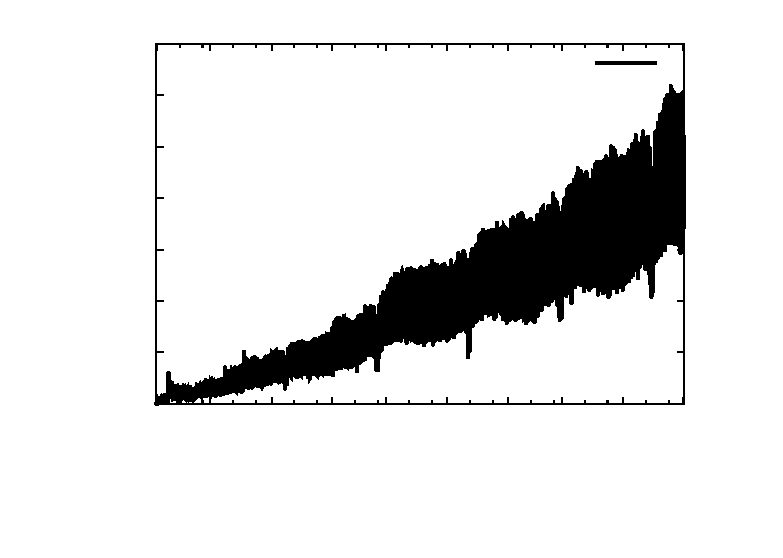
\includegraphics{graphs/requests/questions}}%
    \gplfronttext
  \end{picture}%
\endgroup
}} \quad
  \subfloat[][Answer requests]{\resizebox{0.45\linewidth}{!}{% GNUPLOT: LaTeX picture with Postscript
\begingroup
  \makeatletter
  \providecommand\color[2][]{%
    \GenericError{(gnuplot) \space\space\space\@spaces}{%
      Package color not loaded in conjunction with
      terminal option `colourtext'%
    }{See the gnuplot documentation for explanation.%
    }{Either use 'blacktext' in gnuplot or load the package
      color.sty in LaTeX.}%
    \renewcommand\color[2][]{}%
  }%
  \providecommand\includegraphics[2][]{%
    \GenericError{(gnuplot) \space\space\space\@spaces}{%
      Package graphicx or graphics not loaded%
    }{See the gnuplot documentation for explanation.%
    }{The gnuplot epslatex terminal needs graphicx.sty or graphics.sty.}%
    \renewcommand\includegraphics[2][]{}%
  }%
  \providecommand\rotatebox[2]{#2}%
  \@ifundefined{ifGPcolor}{%
    \newif\ifGPcolor
    \GPcolorfalse
  }{}%
  \@ifundefined{ifGPblacktext}{%
    \newif\ifGPblacktext
    \GPblacktexttrue
  }{}%
  % define a \g@addto@macro without @ in the name:
  \let\gplgaddtomacro\g@addto@macro
  % define empty templates for all commands taking text:
  \gdef\gplbacktext{}%
  \gdef\gplfronttext{}%
  \makeatother
  \ifGPblacktext
    % no textcolor at all
    \def\colorrgb#1{}%
    \def\colorgray#1{}%
  \else
    % gray or color?
    \ifGPcolor
      \def\colorrgb#1{\color[rgb]{#1}}%
      \def\colorgray#1{\color[gray]{#1}}%
      \expandafter\def\csname LTw\endcsname{\color{white}}%
      \expandafter\def\csname LTb\endcsname{\color{black}}%
      \expandafter\def\csname LTa\endcsname{\color{black}}%
      \expandafter\def\csname LT0\endcsname{\color[rgb]{1,0,0}}%
      \expandafter\def\csname LT1\endcsname{\color[rgb]{0,1,0}}%
      \expandafter\def\csname LT2\endcsname{\color[rgb]{0,0,1}}%
      \expandafter\def\csname LT3\endcsname{\color[rgb]{1,0,1}}%
      \expandafter\def\csname LT4\endcsname{\color[rgb]{0,1,1}}%
      \expandafter\def\csname LT5\endcsname{\color[rgb]{1,1,0}}%
      \expandafter\def\csname LT6\endcsname{\color[rgb]{0,0,0}}%
      \expandafter\def\csname LT7\endcsname{\color[rgb]{1,0.3,0}}%
      \expandafter\def\csname LT8\endcsname{\color[rgb]{0.5,0.5,0.5}}%
    \else
      % gray
      \def\colorrgb#1{\color{black}}%
      \def\colorgray#1{\color[gray]{#1}}%
      \expandafter\def\csname LTw\endcsname{\color{white}}%
      \expandafter\def\csname LTb\endcsname{\color{black}}%
      \expandafter\def\csname LTa\endcsname{\color{black}}%
      \expandafter\def\csname LT0\endcsname{\color{black}}%
      \expandafter\def\csname LT1\endcsname{\color{black}}%
      \expandafter\def\csname LT2\endcsname{\color{black}}%
      \expandafter\def\csname LT3\endcsname{\color{black}}%
      \expandafter\def\csname LT4\endcsname{\color{black}}%
      \expandafter\def\csname LT5\endcsname{\color{black}}%
      \expandafter\def\csname LT6\endcsname{\color{black}}%
      \expandafter\def\csname LT7\endcsname{\color{black}}%
      \expandafter\def\csname LT8\endcsname{\color{black}}%
    \fi
  \fi
  \setlength{\unitlength}{0.0500bp}%
  \begin{picture}(7200.00,5040.00)%
    \gplgaddtomacro\gplbacktext{%
      \csname LTb\endcsname%
      \put(1210,1320){\makebox(0,0)[r]{\strut{} 0}}%
      \put(1210,1704){\makebox(0,0)[r]{\strut{} 2000}}%
      \put(1210,2088){\makebox(0,0)[r]{\strut{} 4000}}%
      \put(1210,2472){\makebox(0,0)[r]{\strut{} 6000}}%
      \put(1210,2856){\makebox(0,0)[r]{\strut{} 8000}}%
      \put(1210,3239){\makebox(0,0)[r]{\strut{} 10000}}%
      \put(1210,3623){\makebox(0,0)[r]{\strut{} 12000}}%
      \put(1210,4007){\makebox(0,0)[r]{\strut{} 14000}}%
      \put(1210,4391){\makebox(0,0)[r]{\strut{} 16000}}%
      \put(1210,4775){\makebox(0,0)[r]{\strut{} 18000}}%
      \put(552,352){\rotatebox{45}{\makebox(0,0)[l]{\strut{}01-08-2008}}}%
      \put(1064,352){\rotatebox{45}{\makebox(0,0)[l]{\strut{}01-03-2009}}}%
      \put(1655,352){\rotatebox{45}{\makebox(0,0)[l]{\strut{}01-11-2009}}}%
      \put(2236,352){\rotatebox{45}{\makebox(0,0)[l]{\strut{}01-07-2010}}}%
      \put(2755,352){\rotatebox{45}{\makebox(0,0)[l]{\strut{}01-02-2011}}}%
      \put(3338,352){\rotatebox{45}{\makebox(0,0)[l]{\strut{}01-10-2011}}}%
      \put(3924,352){\rotatebox{45}{\makebox(0,0)[l]{\strut{}01-06-2012}}}%
      \put(4440,352){\rotatebox{45}{\makebox(0,0)[l]{\strut{}01-01-2013}}}%
      \put(5027,352){\rotatebox{45}{\makebox(0,0)[l]{\strut{}01-09-2013}}}%
      \put(5608,352){\rotatebox{45}{\makebox(0,0)[l]{\strut{}01-05-2014}}}%
      \put(176,3047){\rotatebox{-270}{\makebox(0,0){\strut{}Requests}}}%
    }%
    \gplgaddtomacro\gplfronttext{%
      \csname LTb\endcsname%
      \put(5420,4594){\makebox(0,0)[r]{\strut{}Answer}}%
    }%
    \gplbacktext
    \put(0,0){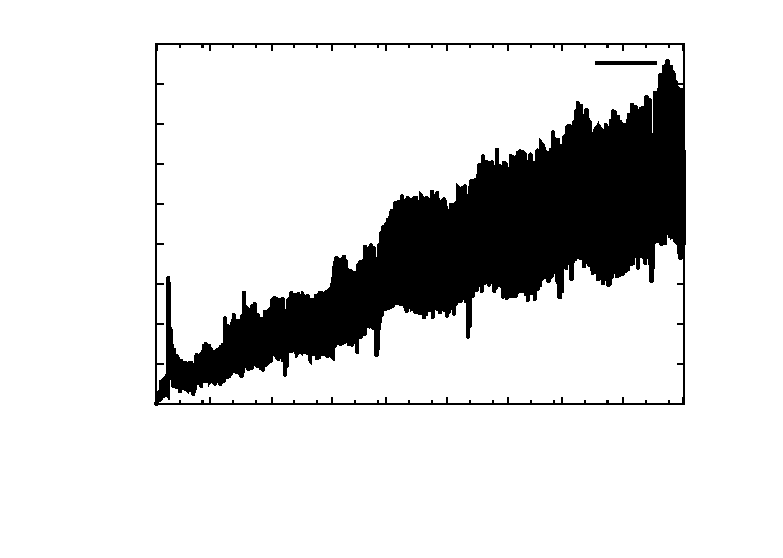
\includegraphics{graphs/requests/answers}}%
    \gplfronttext
  \end{picture}%
\endgroup
}} \\
  \subfloat[][Comment requests]{\resizebox{0.45\linewidth}{!}{% GNUPLOT: LaTeX picture with Postscript
\begingroup
  \makeatletter
  \providecommand\color[2][]{%
    \GenericError{(gnuplot) \space\space\space\@spaces}{%
      Package color not loaded in conjunction with
      terminal option `colourtext'%
    }{See the gnuplot documentation for explanation.%
    }{Either use 'blacktext' in gnuplot or load the package
      color.sty in LaTeX.}%
    \renewcommand\color[2][]{}%
  }%
  \providecommand\includegraphics[2][]{%
    \GenericError{(gnuplot) \space\space\space\@spaces}{%
      Package graphicx or graphics not loaded%
    }{See the gnuplot documentation for explanation.%
    }{The gnuplot epslatex terminal needs graphicx.sty or graphics.sty.}%
    \renewcommand\includegraphics[2][]{}%
  }%
  \providecommand\rotatebox[2]{#2}%
  \@ifundefined{ifGPcolor}{%
    \newif\ifGPcolor
    \GPcolorfalse
  }{}%
  \@ifundefined{ifGPblacktext}{%
    \newif\ifGPblacktext
    \GPblacktexttrue
  }{}%
  % define a \g@addto@macro without @ in the name:
  \let\gplgaddtomacro\g@addto@macro
  % define empty templates for all commands taking text:
  \gdef\gplbacktext{}%
  \gdef\gplfronttext{}%
  \makeatother
  \ifGPblacktext
    % no textcolor at all
    \def\colorrgb#1{}%
    \def\colorgray#1{}%
  \else
    % gray or color?
    \ifGPcolor
      \def\colorrgb#1{\color[rgb]{#1}}%
      \def\colorgray#1{\color[gray]{#1}}%
      \expandafter\def\csname LTw\endcsname{\color{white}}%
      \expandafter\def\csname LTb\endcsname{\color{black}}%
      \expandafter\def\csname LTa\endcsname{\color{black}}%
      \expandafter\def\csname LT0\endcsname{\color[rgb]{1,0,0}}%
      \expandafter\def\csname LT1\endcsname{\color[rgb]{0,1,0}}%
      \expandafter\def\csname LT2\endcsname{\color[rgb]{0,0,1}}%
      \expandafter\def\csname LT3\endcsname{\color[rgb]{1,0,1}}%
      \expandafter\def\csname LT4\endcsname{\color[rgb]{0,1,1}}%
      \expandafter\def\csname LT5\endcsname{\color[rgb]{1,1,0}}%
      \expandafter\def\csname LT6\endcsname{\color[rgb]{0,0,0}}%
      \expandafter\def\csname LT7\endcsname{\color[rgb]{1,0.3,0}}%
      \expandafter\def\csname LT8\endcsname{\color[rgb]{0.5,0.5,0.5}}%
    \else
      % gray
      \def\colorrgb#1{\color{black}}%
      \def\colorgray#1{\color[gray]{#1}}%
      \expandafter\def\csname LTw\endcsname{\color{white}}%
      \expandafter\def\csname LTb\endcsname{\color{black}}%
      \expandafter\def\csname LTa\endcsname{\color{black}}%
      \expandafter\def\csname LT0\endcsname{\color{black}}%
      \expandafter\def\csname LT1\endcsname{\color{black}}%
      \expandafter\def\csname LT2\endcsname{\color{black}}%
      \expandafter\def\csname LT3\endcsname{\color{black}}%
      \expandafter\def\csname LT4\endcsname{\color{black}}%
      \expandafter\def\csname LT5\endcsname{\color{black}}%
      \expandafter\def\csname LT6\endcsname{\color{black}}%
      \expandafter\def\csname LT7\endcsname{\color{black}}%
      \expandafter\def\csname LT8\endcsname{\color{black}}%
    \fi
  \fi
  \setlength{\unitlength}{0.0500bp}%
  \begin{picture}(7200.00,5040.00)%
    \gplgaddtomacro\gplbacktext{%
      \csname LTb\endcsname%
      \put(1210,1320){\makebox(0,0)[r]{\strut{} 0}}%
      \put(1210,1666){\makebox(0,0)[r]{\strut{} 5000}}%
      \put(1210,2011){\makebox(0,0)[r]{\strut{} 10000}}%
      \put(1210,2357){\makebox(0,0)[r]{\strut{} 15000}}%
      \put(1210,2702){\makebox(0,0)[r]{\strut{} 20000}}%
      \put(1210,3048){\makebox(0,0)[r]{\strut{} 25000}}%
      \put(1210,3393){\makebox(0,0)[r]{\strut{} 30000}}%
      \put(1210,3739){\makebox(0,0)[r]{\strut{} 35000}}%
      \put(1210,4084){\makebox(0,0)[r]{\strut{} 40000}}%
      \put(1210,4430){\makebox(0,0)[r]{\strut{} 45000}}%
      \put(1210,4775){\makebox(0,0)[r]{\strut{} 50000}}%
      \put(552,352){\rotatebox{45}{\makebox(0,0)[l]{\strut{}01-08-2008}}}%
      \put(1064,352){\rotatebox{45}{\makebox(0,0)[l]{\strut{}01-03-2009}}}%
      \put(1655,352){\rotatebox{45}{\makebox(0,0)[l]{\strut{}01-11-2009}}}%
      \put(2236,352){\rotatebox{45}{\makebox(0,0)[l]{\strut{}01-07-2010}}}%
      \put(2755,352){\rotatebox{45}{\makebox(0,0)[l]{\strut{}01-02-2011}}}%
      \put(3338,352){\rotatebox{45}{\makebox(0,0)[l]{\strut{}01-10-2011}}}%
      \put(3924,352){\rotatebox{45}{\makebox(0,0)[l]{\strut{}01-06-2012}}}%
      \put(4440,352){\rotatebox{45}{\makebox(0,0)[l]{\strut{}01-01-2013}}}%
      \put(5027,352){\rotatebox{45}{\makebox(0,0)[l]{\strut{}01-09-2013}}}%
      \put(5608,352){\rotatebox{45}{\makebox(0,0)[l]{\strut{}01-05-2014}}}%
      \put(176,3047){\rotatebox{-270}{\makebox(0,0){\strut{}Requests}}}%
    }%
    \gplgaddtomacro\gplfronttext{%
      \csname LTb\endcsname%
      \put(5420,4594){\makebox(0,0)[r]{\strut{}Comment}}%
    }%
    \gplbacktext
    \put(0,0){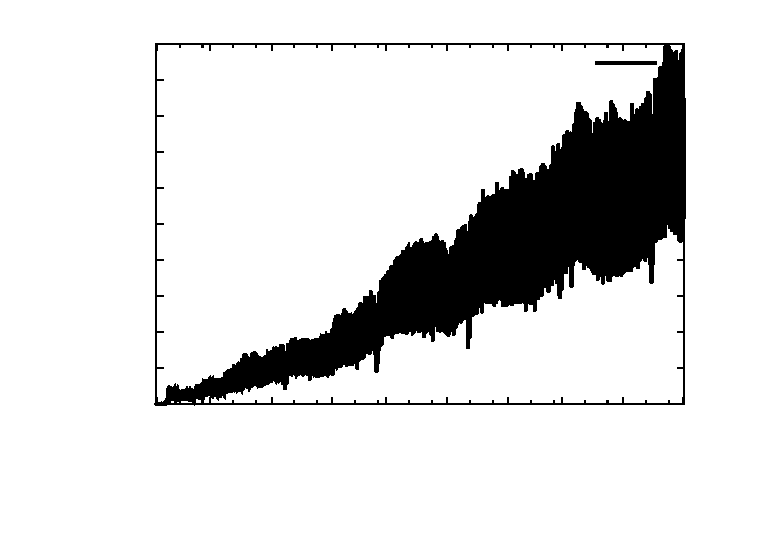
\includegraphics{graphs/requests/comments}}%
    \gplfronttext
  \end{picture}%
\endgroup
}} \quad
  \subfloat[][Vote requests]{\resizebox{0.45\linewidth}{!}{% GNUPLOT: LaTeX picture with Postscript
\begingroup
  \makeatletter
  \providecommand\color[2][]{%
    \GenericError{(gnuplot) \space\space\space\@spaces}{%
      Package color not loaded in conjunction with
      terminal option `colourtext'%
    }{See the gnuplot documentation for explanation.%
    }{Either use 'blacktext' in gnuplot or load the package
      color.sty in LaTeX.}%
    \renewcommand\color[2][]{}%
  }%
  \providecommand\includegraphics[2][]{%
    \GenericError{(gnuplot) \space\space\space\@spaces}{%
      Package graphicx or graphics not loaded%
    }{See the gnuplot documentation for explanation.%
    }{The gnuplot epslatex terminal needs graphicx.sty or graphics.sty.}%
    \renewcommand\includegraphics[2][]{}%
  }%
  \providecommand\rotatebox[2]{#2}%
  \@ifundefined{ifGPcolor}{%
    \newif\ifGPcolor
    \GPcolorfalse
  }{}%
  \@ifundefined{ifGPblacktext}{%
    \newif\ifGPblacktext
    \GPblacktexttrue
  }{}%
  % define a \g@addto@macro without @ in the name:
  \let\gplgaddtomacro\g@addto@macro
  % define empty templates for all commands taking text:
  \gdef\gplbacktext{}%
  \gdef\gplfronttext{}%
  \makeatother
  \ifGPblacktext
    % no textcolor at all
    \def\colorrgb#1{}%
    \def\colorgray#1{}%
  \else
    % gray or color?
    \ifGPcolor
      \def\colorrgb#1{\color[rgb]{#1}}%
      \def\colorgray#1{\color[gray]{#1}}%
      \expandafter\def\csname LTw\endcsname{\color{white}}%
      \expandafter\def\csname LTb\endcsname{\color{black}}%
      \expandafter\def\csname LTa\endcsname{\color{black}}%
      \expandafter\def\csname LT0\endcsname{\color[rgb]{1,0,0}}%
      \expandafter\def\csname LT1\endcsname{\color[rgb]{0,1,0}}%
      \expandafter\def\csname LT2\endcsname{\color[rgb]{0,0,1}}%
      \expandafter\def\csname LT3\endcsname{\color[rgb]{1,0,1}}%
      \expandafter\def\csname LT4\endcsname{\color[rgb]{0,1,1}}%
      \expandafter\def\csname LT5\endcsname{\color[rgb]{1,1,0}}%
      \expandafter\def\csname LT6\endcsname{\color[rgb]{0,0,0}}%
      \expandafter\def\csname LT7\endcsname{\color[rgb]{1,0.3,0}}%
      \expandafter\def\csname LT8\endcsname{\color[rgb]{0.5,0.5,0.5}}%
    \else
      % gray
      \def\colorrgb#1{\color{black}}%
      \def\colorgray#1{\color[gray]{#1}}%
      \expandafter\def\csname LTw\endcsname{\color{white}}%
      \expandafter\def\csname LTb\endcsname{\color{black}}%
      \expandafter\def\csname LTa\endcsname{\color{black}}%
      \expandafter\def\csname LT0\endcsname{\color{black}}%
      \expandafter\def\csname LT1\endcsname{\color{black}}%
      \expandafter\def\csname LT2\endcsname{\color{black}}%
      \expandafter\def\csname LT3\endcsname{\color{black}}%
      \expandafter\def\csname LT4\endcsname{\color{black}}%
      \expandafter\def\csname LT5\endcsname{\color{black}}%
      \expandafter\def\csname LT6\endcsname{\color{black}}%
      \expandafter\def\csname LT7\endcsname{\color{black}}%
      \expandafter\def\csname LT8\endcsname{\color{black}}%
    \fi
  \fi
  \setlength{\unitlength}{0.0500bp}%
  \begin{picture}(7200.00,5040.00)%
    \gplgaddtomacro\gplbacktext{%
      \csname LTb\endcsname%
      \put(1342,1320){\makebox(0,0)[r]{\strut{} 0}}%
      \put(1342,1666){\makebox(0,0)[r]{\strut{} 10000}}%
      \put(1342,2011){\makebox(0,0)[r]{\strut{} 20000}}%
      \put(1342,2357){\makebox(0,0)[r]{\strut{} 30000}}%
      \put(1342,2702){\makebox(0,0)[r]{\strut{} 40000}}%
      \put(1342,3048){\makebox(0,0)[r]{\strut{} 50000}}%
      \put(1342,3393){\makebox(0,0)[r]{\strut{} 60000}}%
      \put(1342,3739){\makebox(0,0)[r]{\strut{} 70000}}%
      \put(1342,4084){\makebox(0,0)[r]{\strut{} 80000}}%
      \put(1342,4430){\makebox(0,0)[r]{\strut{} 90000}}%
      \put(1342,4775){\makebox(0,0)[r]{\strut{} 100000}}%
      \put(684,352){\rotatebox{45}{\makebox(0,0)[l]{\strut{}01-08-2008}}}%
      \put(1182,352){\rotatebox{45}{\makebox(0,0)[l]{\strut{}01-03-2009}}}%
      \put(1758,352){\rotatebox{45}{\makebox(0,0)[l]{\strut{}01-11-2009}}}%
      \put(2324,352){\rotatebox{45}{\makebox(0,0)[l]{\strut{}01-07-2010}}}%
      \put(2829,352){\rotatebox{45}{\makebox(0,0)[l]{\strut{}01-02-2011}}}%
      \put(3398,352){\rotatebox{45}{\makebox(0,0)[l]{\strut{}01-10-2011}}}%
      \put(3968,352){\rotatebox{45}{\makebox(0,0)[l]{\strut{}01-06-2012}}}%
      \put(4471,352){\rotatebox{45}{\makebox(0,0)[l]{\strut{}01-01-2013}}}%
      \put(5042,352){\rotatebox{45}{\makebox(0,0)[l]{\strut{}01-09-2013}}}%
      \put(5608,352){\rotatebox{45}{\makebox(0,0)[l]{\strut{}01-05-2014}}}%
      \put(176,3047){\rotatebox{-270}{\makebox(0,0){\strut{}Requests}}}%
    }%
    \gplgaddtomacro\gplfronttext{%
      \csname LTb\endcsname%
      \put(5420,4594){\makebox(0,0)[r]{\strut{}Vote}}%
    }%
    \gplbacktext
    \put(0,0){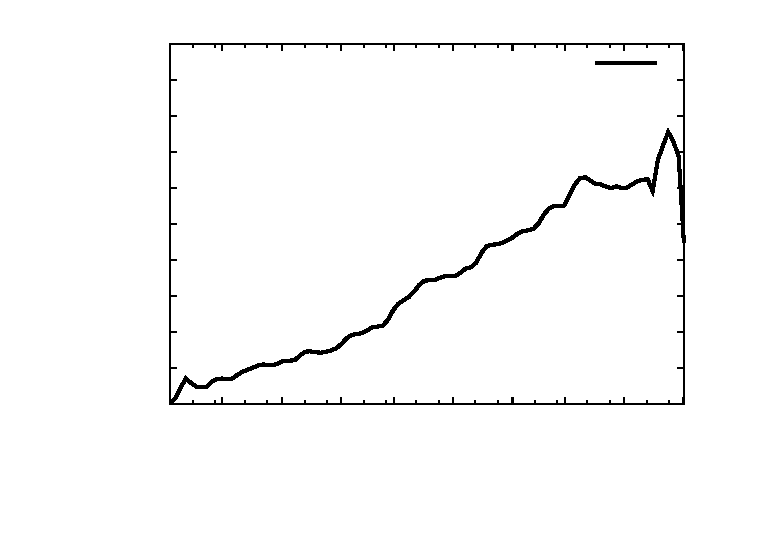
\includegraphics{graphs/requests/votes}}%
    \gplfronttext
  \end{picture}%
\endgroup
}} 
  \subfloat[][Question views]{\resizebox{0.45\linewidth}{!}{% GNUPLOT: LaTeX picture with Postscript
\begingroup
  \makeatletter
  \providecommand\color[2][]{%
    \GenericError{(gnuplot) \space\space\space\@spaces}{%
      Package color not loaded in conjunction with
      terminal option `colourtext'%
    }{See the gnuplot documentation for explanation.%
    }{Either use 'blacktext' in gnuplot or load the package
      color.sty in LaTeX.}%
    \renewcommand\color[2][]{}%
  }%
  \providecommand\includegraphics[2][]{%
    \GenericError{(gnuplot) \space\space\space\@spaces}{%
      Package graphicx or graphics not loaded%
    }{See the gnuplot documentation for explanation.%
    }{The gnuplot epslatex terminal needs graphicx.sty or graphics.sty.}%
    \renewcommand\includegraphics[2][]{}%
  }%
  \providecommand\rotatebox[2]{#2}%
  \@ifundefined{ifGPcolor}{%
    \newif\ifGPcolor
    \GPcolorfalse
  }{}%
  \@ifundefined{ifGPblacktext}{%
    \newif\ifGPblacktext
    \GPblacktexttrue
  }{}%
  % define a \g@addto@macro without @ in the name:
  \let\gplgaddtomacro\g@addto@macro
  % define empty templates for all commands taking text:
  \gdef\gplbacktext{}%
  \gdef\gplfronttext{}%
  \makeatother
  \ifGPblacktext
    % no textcolor at all
    \def\colorrgb#1{}%
    \def\colorgray#1{}%
  \else
    % gray or color?
    \ifGPcolor
      \def\colorrgb#1{\color[rgb]{#1}}%
      \def\colorgray#1{\color[gray]{#1}}%
      \expandafter\def\csname LTw\endcsname{\color{white}}%
      \expandafter\def\csname LTb\endcsname{\color{black}}%
      \expandafter\def\csname LTa\endcsname{\color{black}}%
      \expandafter\def\csname LT0\endcsname{\color[rgb]{1,0,0}}%
      \expandafter\def\csname LT1\endcsname{\color[rgb]{0,1,0}}%
      \expandafter\def\csname LT2\endcsname{\color[rgb]{0,0,1}}%
      \expandafter\def\csname LT3\endcsname{\color[rgb]{1,0,1}}%
      \expandafter\def\csname LT4\endcsname{\color[rgb]{0,1,1}}%
      \expandafter\def\csname LT5\endcsname{\color[rgb]{1,1,0}}%
      \expandafter\def\csname LT6\endcsname{\color[rgb]{0,0,0}}%
      \expandafter\def\csname LT7\endcsname{\color[rgb]{1,0.3,0}}%
      \expandafter\def\csname LT8\endcsname{\color[rgb]{0.5,0.5,0.5}}%
    \else
      % gray
      \def\colorrgb#1{\color{black}}%
      \def\colorgray#1{\color[gray]{#1}}%
      \expandafter\def\csname LTw\endcsname{\color{white}}%
      \expandafter\def\csname LTb\endcsname{\color{black}}%
      \expandafter\def\csname LTa\endcsname{\color{black}}%
      \expandafter\def\csname LT0\endcsname{\color{black}}%
      \expandafter\def\csname LT1\endcsname{\color{black}}%
      \expandafter\def\csname LT2\endcsname{\color{black}}%
      \expandafter\def\csname LT3\endcsname{\color{black}}%
      \expandafter\def\csname LT4\endcsname{\color{black}}%
      \expandafter\def\csname LT5\endcsname{\color{black}}%
      \expandafter\def\csname LT6\endcsname{\color{black}}%
      \expandafter\def\csname LT7\endcsname{\color{black}}%
      \expandafter\def\csname LT8\endcsname{\color{black}}%
    \fi
  \fi
  \setlength{\unitlength}{0.0500bp}%
  \begin{picture}(7200.00,5040.00)%
    \gplgaddtomacro\gplbacktext{%
      \csname LTb\endcsname%
      \put(1474,1320){\makebox(0,0)[r]{\strut{} 0}}%
      \put(1474,1666){\makebox(0,0)[r]{\strut{} 2e+06}}%
      \put(1474,2011){\makebox(0,0)[r]{\strut{} 4e+06}}%
      \put(1474,2357){\makebox(0,0)[r]{\strut{} 6e+06}}%
      \put(1474,2702){\makebox(0,0)[r]{\strut{} 8e+06}}%
      \put(1474,3048){\makebox(0,0)[r]{\strut{} 1e+07}}%
      \put(1474,3393){\makebox(0,0)[r]{\strut{} 1.2e+07}}%
      \put(1474,3739){\makebox(0,0)[r]{\strut{} 1.4e+07}}%
      \put(1474,4084){\makebox(0,0)[r]{\strut{} 1.6e+07}}%
      \put(1474,4430){\makebox(0,0)[r]{\strut{} 1.8e+07}}%
      \put(1474,4775){\makebox(0,0)[r]{\strut{} 2e+07}}%
      \put(816,352){\rotatebox{45}{\makebox(0,0)[l]{\strut{}01-08-2008}}}%
      \put(1301,352){\rotatebox{45}{\makebox(0,0)[l]{\strut{}01-03-2009}}}%
      \put(1861,352){\rotatebox{45}{\makebox(0,0)[l]{\strut{}01-11-2009}}}%
      \put(2412,352){\rotatebox{45}{\makebox(0,0)[l]{\strut{}01-07-2010}}}%
      \put(2904,352){\rotatebox{45}{\makebox(0,0)[l]{\strut{}01-02-2011}}}%
      \put(3457,352){\rotatebox{45}{\makebox(0,0)[l]{\strut{}01-10-2011}}}%
      \put(4012,352){\rotatebox{45}{\makebox(0,0)[l]{\strut{}01-06-2012}}}%
      \put(4502,352){\rotatebox{45}{\makebox(0,0)[l]{\strut{}01-01-2013}}}%
      \put(5057,352){\rotatebox{45}{\makebox(0,0)[l]{\strut{}01-09-2013}}}%
      \put(5608,352){\rotatebox{45}{\makebox(0,0)[l]{\strut{}01-05-2014}}}%
      \put(176,3047){\rotatebox{-270}{\makebox(0,0){\strut{}Requests}}}%
    }%
    \gplgaddtomacro\gplfronttext{%
      \csname LTb\endcsname%
      \put(5420,4594){\makebox(0,0)[r]{\strut{}Views}}%
    }%
    \gplbacktext
    \put(0,0){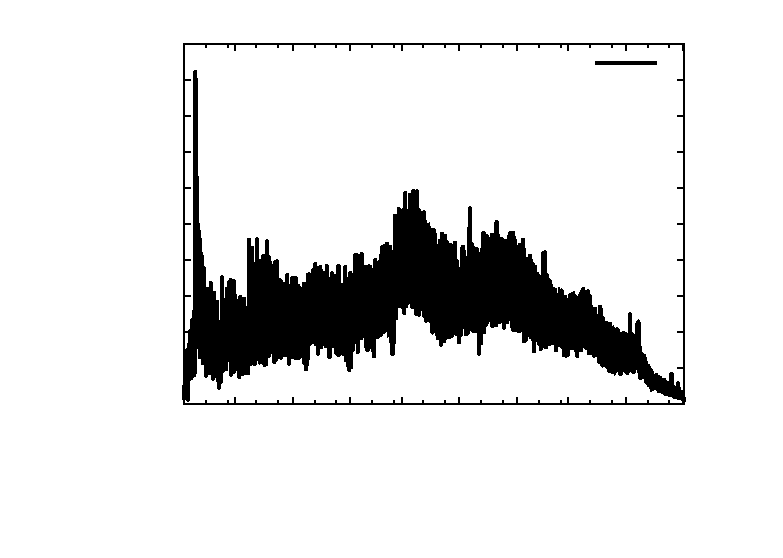
\includegraphics{graphs/requests/views}}%
    \gplfronttext
  \end{picture}%
\endgroup
}} \quad
  \caption{Number of requests per day}
  \label{fig:stackNetworkRequestRate}
\end{figure} 

The Figure \ref{fig:stackNetworkRequestRate} shows the number of new questions, answers and comments per day in the collected data during sampling period. Considering the collected data, we can set a supreme limit of 182 000 \emph{write requests} per day (2 per second if we consider a constant request rate). 

In order to set the throughput expectation for Shuttle, we assume the following request rate ranges for each category of application (Table \ref{tab:base_throughputs}). We consider small-scale applications to retrieve less than 5 million requests per day, enterprise scale retrieve between 5 and 100 million and web scale process from 100 million to billions of requests per day.
For instance, the maximum request arrival rate of one of the Portuguese Ministry of Finances web applications in 2013 was 836 requests per second and 16 million requests in total \cite{opensoft}. In contrast, the total number of requests per day of StackExchange is 148 million (1712 requests per second). We aim that Shuttle fits on current requirements for small and enterprise services. 

\begin{table}[ht]
    \centering
    \begin{tabular}{lr}
      \bf{Category}                          & \bf{Requests per day (Million)}  \\ \hline
      Small                                  & [0, 5[                           \\
      Enterprise                             & [5,100[                          \\
      Portuguese Ministry of Finances        & 16                               \\
      Web scale                              & [100,+$\infty$[                  \\
      StackExchange                          & 148                              \\
    \end{tabular}
    \caption{Throughput per web application category}
    \label{tab:base_throughputs}
\end{table}


%%%%%%%%%%%%%%%%%%%%%%%%%%%%%%%%%%%%%%%%%%%%%%%%%%%%%%%%%%%%%%%%%%%%%%%%%%%%%%%%%%%%%%%%%%%%%%%%%%%%%%%%%%%%%%%%
\section{Precision and Recall}\label{sec:eval:accuracy}

In this Section, we evaluate Shuttle's ability to correctly recover applications by measuring its precision and recall in three categories of intrusion scenarios. \hl{alterei para precision and recall e defini o que significam... é mais lógico do que accuracy}\\

We define precision as the fraction of replayed requests that are legitimate and tainted requests: 

\begin{gather*} 
precision = \frac{ \{tainted \quad requests\} \cap \{replayed \quad requests\}}{\{replayed \quad requests\}}
\end{gather*}

We define recall as the fraction of legitimate and tainted requests that are replayed: 

\begin{gather*} 
recall = \frac{ \{tainted \quad requests\} \cap \{replayed \quad requests\}}{\{tainted \quad requests\}}
\end{gather*}

%Precision measures Shuttle's capability to replay only the tainted requests.
We also may defined precision and recall in terms of malicious and tainted requests. \\

We propose three intrusion scenarios encompass five of the \ac{OWASP} Top 10 Application Security Risks: injection flaws, broken authentication, security misconfiguration, missing function level access control and using components with vulnerabilities \cite{Williams2013}. We consider three classes of intrusion scenarios:

\begin{itemize}
  \item Malicious requests that accidentally or maliciously compromise the application
  \item Software vulnerabilities
  \item External channels (e.g. \ac{SSH} connections)
\end{itemize}

We deployed all Shuttle modules, application instance and database on a single node, a 2.9GHz dual-core Intel i7 with 8GB of memory running the Java 1.7 HotSpot \ac{VM}. This configuration handled, on average, 500 requests per second from a single-thread client. We selected a subset of the \textit{StackExchange Data Dump} \cite{stackexchange_data} containing 100 000 requests originally performed from 31 of July until 12 of September of 2008: 6992 questions, 28 993 questions, 2200 comments, 61 795 votes \LONG{and 3 062 tags}. Requests were sorted per date, establishing 92 939 dependencies. For the sake of simplicity, we ignored view-only requests because the responses to every write requests imply to read the modified question.  

We considered that intrusions happen at 2nd of September, when the database contains 4338 questions, 18286 answers, 422 comments and 38334 votes (61380 requests). The attack is detected in Sep.~12th, assuming a pessimistic delay of 10 days. During this period, the application retrieved 38 620 requests.\\

Table \ref{tab:accuracy} presents a summary of the precision and recall tests. It contains the number of data items tampered by the intrusion (\emph{\#intrusion}) and the number of user requests that read data items written by  tainted requests or malicious requests (without considering the intrusion requests). Recovery using \textit{full replay} requires to replay every request from the latest snapshot before the intrusion instant until the detection instant: in this example at least 38 620 requests (\emph{\#replayed (fr)}). Selective replay only re-executes tainted requests, unless some data item versions need to be recreated. On the worst case, the system does not contain any snapshot and every data read by the tainted requests shall be recreated (\emph{\#replayed (sr)}). Since Shuttle removes all the malicious actions and recovers all the legitimate requests, it has 100\% recall. The selective replay has better precision than full replay because it replays less non tainted requests.

\begin{table}
\centering
\begin{tabular}{l|rrrr}
    & \#intrusion & \#tainted & \#replayed (sr)               & \#replayed (fr)   \\ \hline
1a       & 110          & 0          & [0, 605] (18.18\%)   & > 38 620 (00.28\%)  \\
1b       & 58           & 14         & [0, 379] (18.99\%)   & > 38 620 (00.18\%)  \\
1c       & 48           & 52         & [0, 253] (39.52\%)   & > 38 620 (00.25\%)  \\
2a       & 4 338        & 0          &  -                   & > 38 620 (11.23\%)  \\
2b       & 18 286       & 1 278      &  -                   & > 38 620 (50.67\%)  \\
3        & 2 000        & -          &  -                   & > 38 620 (05.17\%)  \\
\end{tabular}
  \caption{Number of requests replayed during the recovery process and its precision within parenthesis.}
  \label{tab:accuracy}
  \vspace{-5mm}
\end{table}


%We consider an user who performed:
%Before:  2 questions, 48 answers, 0 comments, 0 votes, 1743 views
%After:  14 questions, 144 answers, 29 comments, 0 votes, 60961 views 
%Total: 16 questions, 192 answers, 29 comments, 0 votes, 62704 views 




\subsection{Result consistency}\label{sec:eval:accuracy:consistency}
%discuss what are the expectable results
Shuttle aims to support various \ac{PaaS} applications. Unlike previous works that know the application semantics \cite{undoForOperators}, the semantic of \ac{PaaS} applications is unknown to Shuttle. In order to evaluate the consistency of the results, we need to define the results expected by tenants. 

For instance, if an attacker created a new question and a legitimate user attempts to create a question with the same title. During the replay, the attacker action will be removed. Should the legitimate request be replayed and create the question? On one hand, the user may have created a question with another title but same content. On the other hand, the request contains the title that the user pretended and he may have not created another question. 

Therefore, we argue that developers should consider the application recovery during the design of the application. For instance, if questions are identified by the hash of their text instead of their title, then the legitimate users create a new question only if the text is not equal to the one of other questions. Shuttle does not replay actions which fail during their first execution. In summary, despite Shuttle's consistency \ac{API} (Section \ref{sec:arch:consistency}), developers shall take into consideration the replay process in order to obtain the expected results.\\


Considering the semantics of our \ac{QA} prototype, we identify the expected results on the following most likely attack actions:

\begin{enumerate}
  \item \textbf{Create new question:} The attacker created a new question with a specific title. The following legitimate user requests, which try to create a question with the same title, fail. When the attacker request is removed, the legitimate user requests will perform correctly and create the question. Answers to the removed question will be included in the new question.
  \item \textbf{New answer:} The attacker answer is removed correctly. Since comments to a non-existing answer fail, the comments are also removed.
  \item \textbf{New answer to every question:} Same behavior as to a new answer for a specific question.
  \item \textbf{Modify the question:} The attacker can change the title or the text. The first case is similar to create a new answer. On the second case, Shuttle loads the previous text value.
  \item \textbf{Modify the answer:} If the attacker changes the text, then Shuttle restores the previous text. However, the comments content may become inconsistent with the answer.
  \item \textbf{Delete all questions or answers:} Shuttle restores the deleted data. However, the duplicated questions and answers will fail to create.
\end{enumerate}


\subsection{Malicious Requests}\label{sec:eval:accuracy:requests}
In the first class of scenarios, we consider three cases in which an attacker has stolen an user credential. The attacker uses the stolen credential to impersonate a legitimate user and to perform malicious actions. The method used to obtain the credential is out of the scope of this dissertation. This scenario is similar to a legitimated user who makes usage mistakes.
We consider attackers:

\begin{enumerate}[label=\alph*]
  \item Deleted every question created by the user
  \item Deleted every user answer
  \item Modified every user answer
\end{enumerate}


\textit{1a)} 
%attack
The attacker deletes the user's 4 questions, performing 4 delete requests that remove 106 associated comments and answers. 
%Identify
The tenant identifies the malicious requests through the user session and selects a snapshot previous to the intrusion instant. Users cannot access deleted questions, so no request is tainted. 
%Recover using selective replay
If Shuttle has a snapshot containing the deleted questions, then \textit{selective replay} does not need to replay any request and merges the deleted questions on the current system state. If the latest snapshot is previous to the creation of the 4 questions, then \textit{selective replay} replays 605 requests to recreate the deleted questions, their answers and votes. The result is merged with the current branch, rebuilding the deleted questions. 

To clarify consider the Figure \ref{fig:attack_1_graph} in which the \emph{Req. 4} deletes a question with one answer and one comment. \emph{Req. 4} is a malicious request and the values written by it ($Q1, A1, C1$) need to be removed. If tenant selects the \emph{snapshot B}, then the items $Q1, A1, C1$ are restored to the version before the delete operation and no operation is replayed. If the tenant selects the \emph{snapshot A}, then \emph{Req.1, Req.2, Req.3} are replayed to obtain the value of the $Q1, A1, C1$. 

\begin{figure}
  \centering
  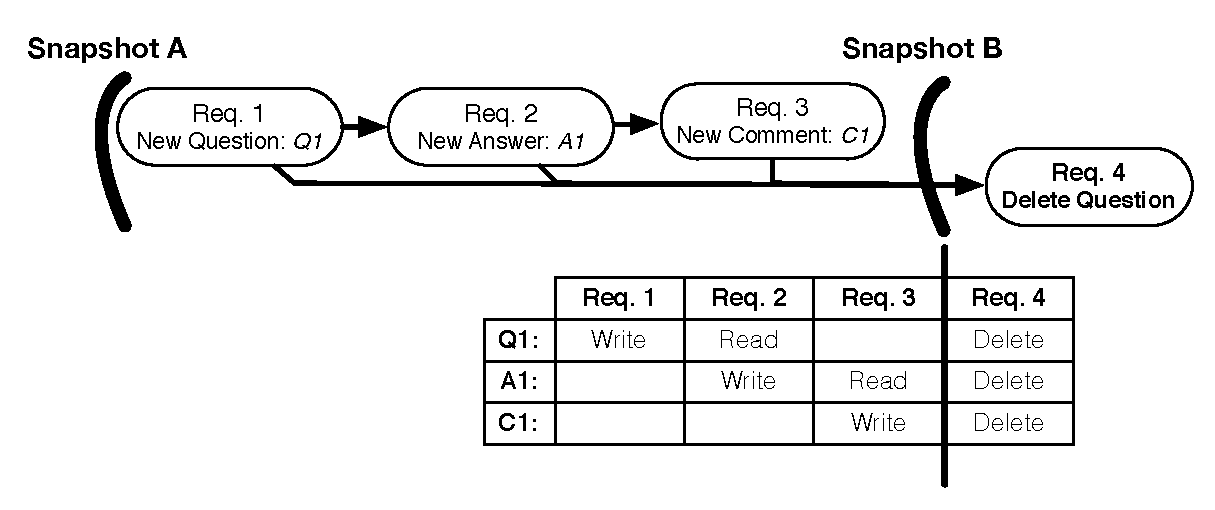
\includegraphics[width=110mm]{images/attack_1_graph}
  \caption[Example of request dependencies]{Example of request dependencies: a malicious request deletes a question with one answer and one comment}
  \label{fig:attack_1_graph}
\end{figure}

The following scenarios are similar.

\textit{1b)} Deleting the user's 48 answers implies that 58 data items are deleted and 14 answers and comments are tainted as they execute after the intrusion instant answering and voting without knowing some answers. If a snapshot containing the user answers exists, then the \textit{selective replay} approach replays only 14 tainted answers and comments. Otherwise, it replays 379 requests: the total number of requests to recreate the tainted questions and then merge the result.

\textit{1c)} 48 data items are modified while 52 requests are tainted because the users replays, votes and comments the modified questions after the intrusion instant. For recovery, the 52 tainted requests shall be replayed. If Shuttle does not have a snapshot containing the questions, then 253 requests have to be replayed to recreate them. 



%%%%%%%%%%%%%%%%%%%%%%%%%%%%%%%%%%%%%%%%%%%%%%%%%%%%%%%%%%%%%%%%%%%%%%%%%%%%%%%%%%%%%%%%%%%%%%%%%%%%%%%%%%%%%%%%%%%%%%%%%%%%%%%%%%%%%%%
\subsection{Software Vulnerability}\label{sec:eval:accuracy:software}
On the second class, we evaluate intrusion scenarios where software flaws allow attackers to modify the database without authorization. For instance, a code version added a flaw that allows \emph{SQL-Injection}. We consider two independent scenarios where the attacker:

\begin{enumerate}[label=\alph*]
  \item Deleted every question
  \item Deleted every answer
\end{enumerate}


In \textit{2a)}, the deleting of every question removes 4 338 data items. In \textit{2b)}, the questions are preserved but 1 278 answers, votes and comments are tainted as the user did not see the deleted answers.


%The attacker replaced the application version by one that accepts unauthenticated requests and stores random data items in the database. Under these circumstances, the intrusion effects are unknown.

Instead of identifying the requests that explored the vulnerability, the tenant patches the code to remove the application vulnerability. The instance rejuvenation mechanism terminates the current application instances and deploys the newest application version (Section \ref{sec:arch:image_rejuvenation}). Then, they use the \textit{full replay} to repeat all requests since the beginning of usage of the software version with the flaw. Requests that explored the vulnerability fail to execute and a consistent application state is recovered.\\

%Extra-cases: 1
Shuttle can also be used to perform preventive updates. Consider the following case: the security team considered that: a) every answer shall be ciphered using the username; b) users without weak-passwords shall not be allowed to answer questions. The development team can rapidly develop a new software version fixing these vulnerabilities. Without Shuttle the system administrator would need to create a script to make the database consistent with the new software version. Shuttle can remove these steps, which require extensive human intervention, by replaying every user request.

\subsection{External Channels}\label{sec:eval:accuracy:external}
On the third class of intrusion scenarios, we consider a case where the proxy does not log the attacker actions. In this section, we propose how to recover from a shellshock attack using Shuttle.

%Shellshock resume
Shellsock vulnerability allows an attacker to execute commands that are interpreted by the bash, i.e., perform code injection. When an attacker sends a \ac{HTTP} request containing the header \emph{User-Agent: () \{ :; \}; <malicious command>} and the web server passes this header field as a bash variable, the bash interprets the malicious command. For sake of clarity, we omit further details. In summary, this vulnerability allows a \ac{HTTP} request to run bash commands.

%Attack
We consider a case in which an attacker used an \ac{HTTP} request to create a new \ac{SSH} user account in one application server. Then, the attacker established a \ac{SSH} connection to an application server using the new user. The attacker stolen a database credentials stored in the application code. The attacker used the credentials to modify at least 2000 data items bypassing Shuttle's database proxy. As consequence, the database operations are not logged and the number of tainted requests is unknown.

%Solution
Tenants can use Shuttle as a request logger to detect the string that exploits the shellshock vulnerability: \emph{() \{:;\};}. If an intrusion is detected, the tenant selects a snapshot previous to the request creation, which does not contain data tampered by the intrusion. Since the application instances can be tampered, Shuttle uses the instance rejuvenation mechanism to terminate these instances and redeploy the application in new instances, in which the shellshock vulnerability is fixed.

%Requests are not logged
Shuttle removes the attack effects and recovers the application consistency performing \emph{full replay}. It loads a full database snapshot instead of undoing operations. As consequence, even non-logged operations are undo. Then it replays every HTTP request posterior to the snapshot instant. Since malicious actions were not logged, they are not replayed.\\

The described scenario assumes that Shuttle's trusted computing base is not compromised.

\subsection{Discussion}\label{sec:eval:accuracy:discussion}
The number of requests to replay is defined by the snapshot instant: on \textit{full replay} Shuttle replays all requests performed after the intrusion instant, while on \textit{selective replay} Shuttle replays the requests necessary to read the values of the entries before the intrusion and the tainted requests. While \textit{selective replay} seems to have a big advantage comparing with  \textit{full replay}, which performs, in these scenarios, at least 38 620 requests, most real applications have more dependencies thus the number of tainted requests is bigger. For instance, if the order between questions with the same tag is considered as a dependency,  the number of dependencies rises from 92 939 to 109 118 and the number of independent clusters decreases from 6992 to 56. We plan to further analyze the dependencies established by different types of applications.



% atacante não está logado (mas consegue fazer operações de algum modo)
% \hl{explicar bem o que é o perimetro de seguranca, o que é quebrar esse perimetro e conseguir modificar as instancias. Explicar que o Shuttle nao pode ser comprometido.}
% \textbf{Background:} The prototype \ac{QA} application displays the data that is stored in the database. In this scenario, an attacker is not logged on the application but exploits a container or application vulnerability to gain access to the Voldemort database and modifies a random set of data items without proper authorization. The database may be replicated and the application may use a byzantine fault tolerance mechanism. However, here, we ignore these mechanisms and assume a single non-replicated database.

% The attacker may create questions or answer, create an answer for every question, modify question or answer, delete all questions or answers or even randomly modify part of the database entries or delete every database entry. If the attacker actions were known, the tenant could revert them manually. However, it is arguably hard to track the attacker actions. 

% Even so, the tenant can estimate when the intrusion occurred and if the attacker used application requests or external actions. To do so, the tenant can use Shuttle not only to compare the checkpoints but also to detect database entries without associated requests. Since Shuttle keeps the records on its persistent state of the requests number that accessed each entry, if the attacker creates new entries without using the database \acAPI}, the new entries will not have a consistent sequence of requests. 

% Attacks using user requests are handled in Section \ref{sec:eval:consistency:corrupted_requests}. If the attacker used external actions, the tenant chooses a snapshot previous to the estimated intrusion moment and uses Shuttle to replay the requests after the snapshot. The external actions are not logged, thus not performed, and their effects are removed by loading the snapshot. The tenant may check the recovery process result in a separate branch before publish the results. The number of requests to replay depends only from the estimated intrusion moment and the snapshot previous to that moment. \\


% \textbf{Simulation:} To simulate this case, we executed the first \hl{XX} weeks of the StackExchange \hl{tem de dizer acima as quantidades de cada} to generate the result of an intrusion-less execution. Then, to simulate the attack, we executed the first \hl{XX} weeks and performed a set of intrusive actions directly on the database. Then, to simulate the attack effects, we performed the remaining weeks. Each attack created tampered an arbitrary set of data items of the database. Each attack was repeated 25 times, the standard deviation is presented between square brackets. 

% \textbf{Results:} The intrusion results are presented in Table \ref{fig:eval:scenarioA}.

% \begin{table}[ht]
%   \begin{tabular}{|p{2.6cm}|p{2.5cm}|p{2.5cm}|p{2.5cm}|p{2.5cm}|p{2.5cm}|p{2.5cm}}
%   \textbf{Attack}                 & \textbf{Affected Requests}  & \textbf{Number of Views} & \textbf{How many requests to repeat?} & \textbf{How many repeated?} &  \\ \cline{1-6}
%   Create question                 & The answers and same tags   &  -                       & 0                                     &  After the snapshot                   &  \\ \cline{1-6}
%   Create answer                   & The question and following answers and comments        & Same as question after the date        & 0          & After the snapshot                   &  \\ \hline
%   Create answer to every question &                   &                 &                              &                    &  \\ \cline{1-6}
%   Modify question                 &                   &                 &                              &                    &  \\ \cline{1-6}
%   Modify answer                   &                   &                 &                              &                    &  \\ \cline{1-6}
%   Delete all questions            &                   &                 &                              &                    &  \\ \cline{1-6}
%   Delete all answers              &                   &                 &                              &                    &  \\ \cline{1-6}
%   \end{tabular}
%   \caption{Results of intrusion scenario A}
%   \label{fig:eval:scenarioA}
% \end{table}

% intrusion compromised \hl{XXX}\% of entries in each store. \hl{XXXX} questions (\hl{XXX}\% of total) where affected.
% Random writes on \hl{XXX}\% of entries in each store 
% Qual o pedido antigo mais afetado?
% Quantos pedidos posteriores foram afectados? Quantas vezes foi visto o erro?
% Quantos pedidos tem de ser repetidos? Quantos foram repetidos?
% The attack compromised the actions performed by \hl{XXX} requests. The oldest affected request has been performed at \hl{XXXX December of XXXXX}. \hl{XXX}\% of the requests after that date were affected. Since Shuttle replays every action, the request replay precision is \hl{xxxxx}\%. The recall is 1 since every affected entry is repaired.

% Performing the selective replay of the affected requests, we the precision is \hl{XXXX} and the recall \hl{XXXX}. 

%The intrusions on these scenarios compromise the \ac{PaaS} containers and/or the database. Shuttle recovers from the firsts removing the compromised containers and their attached persistent storage and then launching a new container using a new clean image and deploying the application code (Section \ref{sec:arch:image_recovery}). The remaining attacks, which this section is about, involve database using external actions or using the application requests. The following sections propose different scenarios.


%15.  Qual a disponibilidade da aplicacao:  baseado no grafo anterior mas os items da base de dados sao pesados consoante o numero de views que tem: se tiverem mais views e nao estiverem disponiveis, tem mais peso do que se tiverem menos views.




%---------------------------------- damage propagation ----------------------------------
% Gráfico com a propagacao dos danos causados consante a aplicacao: uma operação é dependente de X operações com probabilidade de X. Considerando que um set de X entradas fica tainted após X entradas, como é que se propaga? Gráfico com o non-tainted vs tainted. Indicar o numero de clusters no final.

% Fazer o save de dados para evitar o redo é dificil de prever se melhora ou nao, depende do grau de indepedencia. Se for aleatorio, os pedidos rapidamente afectam toda a base de dados. xxxxxx justificar com os dados da tabela. Se os dados forem separados, tende a haver isolamento em clusters. Nesse caso, se os clusters sao grandes, entao compensa mas basta haver 1 pedido malicioso para comprometer um cluster. Nesse caso, demora mais fazer o undo selectivo do que o redo all.

%!TEX root = ../tese.tex
%!TEX encoding = UTF-8 Unicode
\section{Overhead}\label{sec:eval:peformance}

The performance evaluation aims to prove Shuttle scalability and capability to support small and enterprise applications (Section \ref{sec:eval:test_description}). Its results should match the evaluation metrics bounds that allow to use Shuttle in real environments. We evaluate Shuttle's performance considering the throughput of the application, the size of the logs and the recovery time. We also estimate the cost of deployment of Shuttle on a public cloud provider (AWS \cite{aws}). \\

We run Shuttle in \acf{AWS}. All instances are connected by gigabit ethernet (780Mbps measured with \emph{iperf}, 0.176ms round-trip time measured with \emph{ping}) and have the \emph{Java 1.7 HotSpot} 64-Bit Server \ac{VM} version installed. Even when the \ac{JVM} performance increases as the bytecode is compiled by the \ac{JIT} compiler, we run every test on new \ac{JVM} instances. They have a 32GB local general purpose \ac{SSD}. We used the local \ac{SSD} since its performance on read is better than a 500 Provisioned \ac{IOPS} \ac{SSD} of 25GB \ref{tab:disk_throughput}. We allocated 5GB of heap to the \ac{JVM} and we disabled database replication (each data item is stored in one data node). \hl{o sistema de replicacao de base de dados foi desactivado}

\begin{table}[ht]
\centering
\begin{tabular}{l|rrrrr}
                   & \multicolumn{1}{l}{\textbf{putc()}} & \multicolumn{1}{l}{\textbf{Block Write}} & \multicolumn{1}{l}{\textbf{Create,Change,Rewrite}} & \multicolumn{1}{l}{\textbf{getc()}} & \multicolumn{1}{l}{\textbf{Block Read}}  \\ \hline
\textbf{EBS SSD}      & 631                                 & 83264                                    & 44448                                              & 1562                                & 105723                                  \\
\textbf{Local SSD} & 619                                 & 106546                                   & 186204                                             & 1577                                & 614790                                 
\end{tabular}
\caption[Comparison between a EBS Provisioned IOPS (SSD) and local SSD instance]{Comparison between a EBS Provisioned IOPS (SSD), which supports up to 500 IOPS, and a local SSD instance using bonnie++ (KB/s)}
\label{tab:disk_throughput}
\end{table}




%%%%%%%%%%%%%%%%%%%%%%%%%%%%%%%%%%%%%%%%%%%%%%%%%%%%%%%%%%%%%%%%%%%%%%%%%%%%%%%%%%%%%%%%%%%%%%%%%%%%%%%%%%%%%%%%
\subsection{Performance Overhead}\label{sec:eval:performance}
In this section, we quantify the overhead imposed by each component of Shuttle.

\subsubsection{Database}\label{sec:eval:performance:database}
We measured the overhead of Shuttle on database instances. We expected it to be the major impact of Shuttle because Shuttle logs every operation. We used \acf{YCSB} \cite{ycsb}. \ac{YCSB} was developed to measure the performance of the new generation of cloud data serving systems, such as Voldemort used in Shuttle. We extended \ac{YCSB} to support the latest version of Voldemort and to use \acf{protobuf} as request format.\\

We used 6 \textit{m3.large} instances (7 \ac{ECU}s, 2 vCPUs, 2.8 GHz, Intel Xeon E5-2680v2, 3.75 GiB memory, 2 x 16 GiB Storage Capacity) to run each database node. The database service was accessed by two \textit{c3.xlarge} instances (14 \ac{ECU}s, 4 vCPUs, 2.8 GHz, Intel Xeon E5-2680v2, 7.5 GB of memory, 2 x 40 GB Storage Capacity).\\


We ran 4 out of 5 workloads (Table \ref{tab:workload_description}) proposed \emph{in} \cite{ycsb}. Workload E (Short ranges) is not supported by Voldemort. \hl{deixei apenas na tabela, iria estar a ler a tabela...} Our database consisted of 60 million 1KB record (total database size: 60GB). Each instance thus had an average of 10GB of data, more than it could cache entirely in memory. Read operations retrieve entire records, while update operations modify one of the ten record fields \cite{ycsb}.

\begin{table}[ht]
\centering
\begin{tabular}{p{0.18\linewidth}p{0.15\linewidth}p{0.09\linewidth}p{0.48\linewidth}}
\textbf{Workload}       & \textbf{Operations}                   & \textbf{Key \newline Selection} & \textbf{Application Example} \\ \hline
A - Update heavy        & Read: 50\% \newline Update: 50\%               & Zipfian                & Session store recording recent actions\\ \hline
B - Read mostly         & Read: 95\% \newline Update: 5\%                & Zipfian                & Photo tagging; add a tag is an update, but most operations are to read tags\\ \hline
C - Read only           & Read: 100\%                           & Zipfian                & User profile cache, where profiles are constructed elsewhere (e.g., Hadoop)\\ \hline
D - Read latest         & Read: 95\% \newline Insert: 5\%                & Latest                 & User status updates; people want to read the latest \\ \hline
% F - Read-modify-write  & Get: 50\%  \newline Read-modify-write: 50\%    & Zipfian                & User database, where user records are read and modified by the user or to record user activity.\\ \hline

\end{tabular}
\caption{Workload description}
\label{tab:workload_description}
\end{table}


\begin{figure}[!htb]
  \centering
  \subfloat[][\textbf{Workload A:} read operations]{\resizebox{0.45\linewidth}{!}{% GNUPLOT: LaTeX picture with Postscript
\begingroup
  \makeatletter
  \providecommand\color[2][]{%
    \GenericError{(gnuplot) \space\space\space\@spaces}{%
      Package color not loaded in conjunction with
      terminal option `colourtext'%
    }{See the gnuplot documentation for explanation.%
    }{Either use 'blacktext' in gnuplot or load the package
      color.sty in LaTeX.}%
    \renewcommand\color[2][]{}%
  }%
  \providecommand\includegraphics[2][]{%
    \GenericError{(gnuplot) \space\space\space\@spaces}{%
      Package graphicx or graphics not loaded%
    }{See the gnuplot documentation for explanation.%
    }{The gnuplot epslatex terminal needs graphicx.sty or graphics.sty.}%
    \renewcommand\includegraphics[2][]{}%
  }%
  \providecommand\rotatebox[2]{#2}%
  \@ifundefined{ifGPcolor}{%
    \newif\ifGPcolor
    \GPcolorfalse
  }{}%
  \@ifundefined{ifGPblacktext}{%
    \newif\ifGPblacktext
    \GPblacktexttrue
  }{}%
  % define a \g@addto@macro without @ in the name:
  \let\gplgaddtomacro\g@addto@macro
  % define empty templates for all commands taking text:
  \gdef\gplbacktext{}%
  \gdef\gplfronttext{}%
  \makeatother
  \ifGPblacktext
    % no textcolor at all
    \def\colorrgb#1{}%
    \def\colorgray#1{}%
  \else
    % gray or color?
    \ifGPcolor
      \def\colorrgb#1{\color[rgb]{#1}}%
      \def\colorgray#1{\color[gray]{#1}}%
      \expandafter\def\csname LTw\endcsname{\color{white}}%
      \expandafter\def\csname LTb\endcsname{\color{black}}%
      \expandafter\def\csname LTa\endcsname{\color{black}}%
      \expandafter\def\csname LT0\endcsname{\color[rgb]{1,0,0}}%
      \expandafter\def\csname LT1\endcsname{\color[rgb]{0,1,0}}%
      \expandafter\def\csname LT2\endcsname{\color[rgb]{0,0,1}}%
      \expandafter\def\csname LT3\endcsname{\color[rgb]{1,0,1}}%
      \expandafter\def\csname LT4\endcsname{\color[rgb]{0,1,1}}%
      \expandafter\def\csname LT5\endcsname{\color[rgb]{1,1,0}}%
      \expandafter\def\csname LT6\endcsname{\color[rgb]{0,0,0}}%
      \expandafter\def\csname LT7\endcsname{\color[rgb]{1,0.3,0}}%
      \expandafter\def\csname LT8\endcsname{\color[rgb]{0.5,0.5,0.5}}%
    \else
      % gray
      \def\colorrgb#1{\color{black}}%
      \def\colorgray#1{\color[gray]{#1}}%
      \expandafter\def\csname LTw\endcsname{\color{white}}%
      \expandafter\def\csname LTb\endcsname{\color{black}}%
      \expandafter\def\csname LTa\endcsname{\color{black}}%
      \expandafter\def\csname LT0\endcsname{\color{black}}%
      \expandafter\def\csname LT1\endcsname{\color{black}}%
      \expandafter\def\csname LT2\endcsname{\color{black}}%
      \expandafter\def\csname LT3\endcsname{\color{black}}%
      \expandafter\def\csname LT4\endcsname{\color{black}}%
      \expandafter\def\csname LT5\endcsname{\color{black}}%
      \expandafter\def\csname LT6\endcsname{\color{black}}%
      \expandafter\def\csname LT7\endcsname{\color{black}}%
      \expandafter\def\csname LT8\endcsname{\color{black}}%
    \fi
  \fi
  \setlength{\unitlength}{0.0500bp}%
  \begin{picture}(7200.00,5040.00)%
    \gplgaddtomacro\gplbacktext{%
      \csname LTb\endcsname%
      \put(1078,704){\makebox(0,0)[r]{\strut{} 0}}%
      \put(1078,1629){\makebox(0,0)[r]{\strut{} 500}}%
      \put(1078,2554){\makebox(0,0)[r]{\strut{} 1000}}%
      \put(1078,3480){\makebox(0,0)[r]{\strut{} 1500}}%
      \put(1078,4405){\makebox(0,0)[r]{\strut{} 2000}}%
      \put(1210,484){\makebox(0,0){\strut{} 0}}%
      \put(1909,484){\makebox(0,0){\strut{} 5}}%
      \put(2608,484){\makebox(0,0){\strut{} 10}}%
      \put(3307,484){\makebox(0,0){\strut{} 15}}%
      \put(4007,484){\makebox(0,0){\strut{} 20}}%
      \put(4706,484){\makebox(0,0){\strut{} 25}}%
      \put(5405,484){\makebox(0,0){\strut{} 30}}%
      \put(6104,484){\makebox(0,0){\strut{} 35}}%
      \put(6803,484){\makebox(0,0){\strut{} 40}}%
      \put(176,2739){\rotatebox{-270}{\makebox(0,0){\strut{}Read latency (us)}}}%
      \put(4006,154){\makebox(0,0){\strut{}Throughput (thousand ops/sec)}}%
    }%
    \gplgaddtomacro\gplfronttext{%
      \csname LTb\endcsname%
      \put(5816,1416){\makebox(0,0)[r]{\strut{}Shuttle}}%
      \csname LTb\endcsname%
      \put(5816,1042){\makebox(0,0)[r]{\strut{}No Shuttle}}%
    }%
    \gplbacktext
    \put(0,0){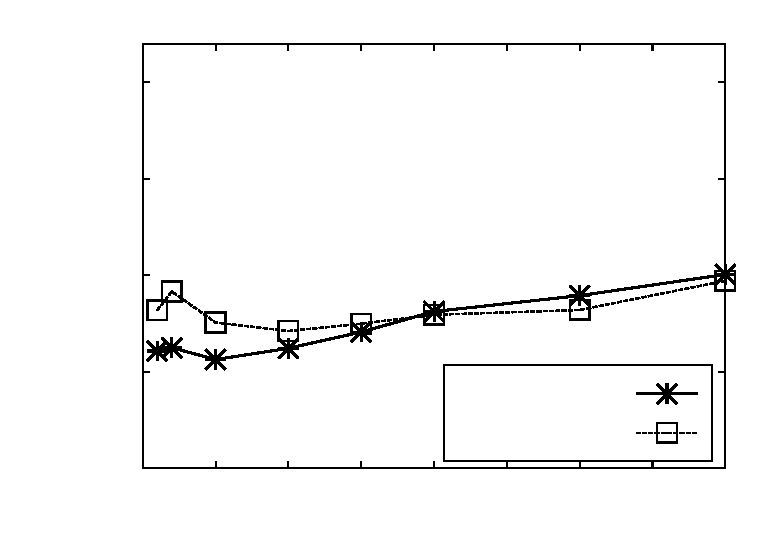
\includegraphics{graphs/database/a_read}}%
    \gplfronttext
  \end{picture}%
\endgroup
}} 
  \subfloat[][\textbf{Workload A:} update operations]{\resizebox{0.45\linewidth}{!}{% GNUPLOT: LaTeX picture with Postscript
\begingroup
  \makeatletter
  \providecommand\color[2][]{%
    \GenericError{(gnuplot) \space\space\space\@spaces}{%
      Package color not loaded in conjunction with
      terminal option `colourtext'%
    }{See the gnuplot documentation for explanation.%
    }{Either use 'blacktext' in gnuplot or load the package
      color.sty in LaTeX.}%
    \renewcommand\color[2][]{}%
  }%
  \providecommand\includegraphics[2][]{%
    \GenericError{(gnuplot) \space\space\space\@spaces}{%
      Package graphicx or graphics not loaded%
    }{See the gnuplot documentation for explanation.%
    }{The gnuplot epslatex terminal needs graphicx.sty or graphics.sty.}%
    \renewcommand\includegraphics[2][]{}%
  }%
  \providecommand\rotatebox[2]{#2}%
  \@ifundefined{ifGPcolor}{%
    \newif\ifGPcolor
    \GPcolorfalse
  }{}%
  \@ifundefined{ifGPblacktext}{%
    \newif\ifGPblacktext
    \GPblacktexttrue
  }{}%
  % define a \g@addto@macro without @ in the name:
  \let\gplgaddtomacro\g@addto@macro
  % define empty templates for all commands taking text:
  \gdef\gplbacktext{}%
  \gdef\gplfronttext{}%
  \makeatother
  \ifGPblacktext
    % no textcolor at all
    \def\colorrgb#1{}%
    \def\colorgray#1{}%
  \else
    % gray or color?
    \ifGPcolor
      \def\colorrgb#1{\color[rgb]{#1}}%
      \def\colorgray#1{\color[gray]{#1}}%
      \expandafter\def\csname LTw\endcsname{\color{white}}%
      \expandafter\def\csname LTb\endcsname{\color{black}}%
      \expandafter\def\csname LTa\endcsname{\color{black}}%
      \expandafter\def\csname LT0\endcsname{\color[rgb]{1,0,0}}%
      \expandafter\def\csname LT1\endcsname{\color[rgb]{0,1,0}}%
      \expandafter\def\csname LT2\endcsname{\color[rgb]{0,0,1}}%
      \expandafter\def\csname LT3\endcsname{\color[rgb]{1,0,1}}%
      \expandafter\def\csname LT4\endcsname{\color[rgb]{0,1,1}}%
      \expandafter\def\csname LT5\endcsname{\color[rgb]{1,1,0}}%
      \expandafter\def\csname LT6\endcsname{\color[rgb]{0,0,0}}%
      \expandafter\def\csname LT7\endcsname{\color[rgb]{1,0.3,0}}%
      \expandafter\def\csname LT8\endcsname{\color[rgb]{0.5,0.5,0.5}}%
    \else
      % gray
      \def\colorrgb#1{\color{black}}%
      \def\colorgray#1{\color[gray]{#1}}%
      \expandafter\def\csname LTw\endcsname{\color{white}}%
      \expandafter\def\csname LTb\endcsname{\color{black}}%
      \expandafter\def\csname LTa\endcsname{\color{black}}%
      \expandafter\def\csname LT0\endcsname{\color{black}}%
      \expandafter\def\csname LT1\endcsname{\color{black}}%
      \expandafter\def\csname LT2\endcsname{\color{black}}%
      \expandafter\def\csname LT3\endcsname{\color{black}}%
      \expandafter\def\csname LT4\endcsname{\color{black}}%
      \expandafter\def\csname LT5\endcsname{\color{black}}%
      \expandafter\def\csname LT6\endcsname{\color{black}}%
      \expandafter\def\csname LT7\endcsname{\color{black}}%
      \expandafter\def\csname LT8\endcsname{\color{black}}%
    \fi
  \fi
  \setlength{\unitlength}{0.0500bp}%
  \begin{picture}(7200.00,5040.00)%
    \gplgaddtomacro\gplbacktext{%
      \csname LTb\endcsname%
      \put(1078,704){\makebox(0,0)[r]{\strut{} 0}}%
      \put(1078,1629){\makebox(0,0)[r]{\strut{} 500}}%
      \put(1078,2554){\makebox(0,0)[r]{\strut{} 1000}}%
      \put(1078,3480){\makebox(0,0)[r]{\strut{} 1500}}%
      \put(1078,4405){\makebox(0,0)[r]{\strut{} 2000}}%
      \put(1210,484){\makebox(0,0){\strut{} 5}}%
      \put(2009,484){\makebox(0,0){\strut{} 10}}%
      \put(2808,484){\makebox(0,0){\strut{} 15}}%
      \put(3607,484){\makebox(0,0){\strut{} 20}}%
      \put(4406,484){\makebox(0,0){\strut{} 25}}%
      \put(5205,484){\makebox(0,0){\strut{} 30}}%
      \put(6004,484){\makebox(0,0){\strut{} 35}}%
      \put(6803,484){\makebox(0,0){\strut{} 40}}%
      \put(176,2739){\rotatebox{-270}{\makebox(0,0){\strut{}Update latency (us)}}}%
      \put(4006,154){\makebox(0,0){\strut{}Throughput (thousand ops/sec)}}%
    }%
    \gplgaddtomacro\gplfronttext{%
      \csname LTb\endcsname%
      \put(5816,1416){\makebox(0,0)[r]{\strut{}Shuttle}}%
      \csname LTb\endcsname%
      \put(5816,1042){\makebox(0,0)[r]{\strut{}No Shuttle}}%
    }%
    \gplbacktext
    \put(0,0){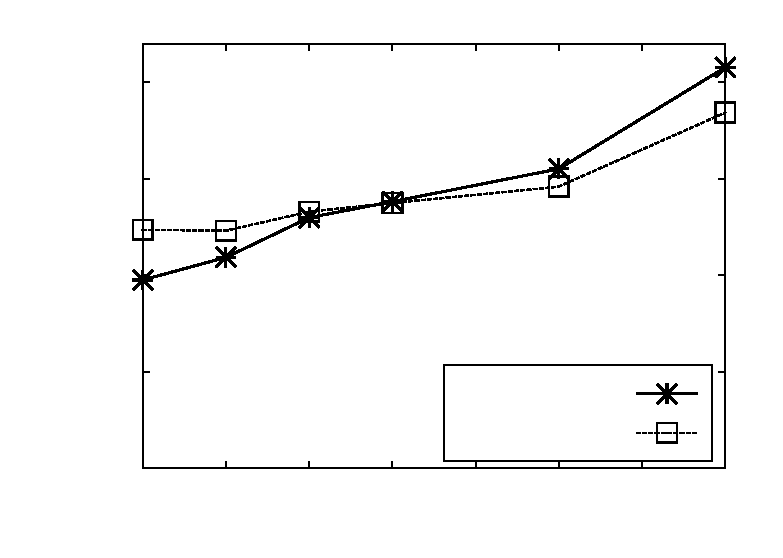
\includegraphics{graphs/database/a_update}}%
    \gplfronttext
  \end{picture}%
\endgroup
}}

  \subfloat[][\textbf{Workload B:} read operations]{\resizebox{0.45\linewidth}{!}{% GNUPLOT: LaTeX picture with Postscript
\begingroup
  \makeatletter
  \providecommand\color[2][]{%
    \GenericError{(gnuplot) \space\space\space\@spaces}{%
      Package color not loaded in conjunction with
      terminal option `colourtext'%
    }{See the gnuplot documentation for explanation.%
    }{Either use 'blacktext' in gnuplot or load the package
      color.sty in LaTeX.}%
    \renewcommand\color[2][]{}%
  }%
  \providecommand\includegraphics[2][]{%
    \GenericError{(gnuplot) \space\space\space\@spaces}{%
      Package graphicx or graphics not loaded%
    }{See the gnuplot documentation for explanation.%
    }{The gnuplot epslatex terminal needs graphicx.sty or graphics.sty.}%
    \renewcommand\includegraphics[2][]{}%
  }%
  \providecommand\rotatebox[2]{#2}%
  \@ifundefined{ifGPcolor}{%
    \newif\ifGPcolor
    \GPcolorfalse
  }{}%
  \@ifundefined{ifGPblacktext}{%
    \newif\ifGPblacktext
    \GPblacktexttrue
  }{}%
  % define a \g@addto@macro without @ in the name:
  \let\gplgaddtomacro\g@addto@macro
  % define empty templates for all commands taking text:
  \gdef\gplbacktext{}%
  \gdef\gplfronttext{}%
  \makeatother
  \ifGPblacktext
    % no textcolor at all
    \def\colorrgb#1{}%
    \def\colorgray#1{}%
  \else
    % gray or color?
    \ifGPcolor
      \def\colorrgb#1{\color[rgb]{#1}}%
      \def\colorgray#1{\color[gray]{#1}}%
      \expandafter\def\csname LTw\endcsname{\color{white}}%
      \expandafter\def\csname LTb\endcsname{\color{black}}%
      \expandafter\def\csname LTa\endcsname{\color{black}}%
      \expandafter\def\csname LT0\endcsname{\color[rgb]{1,0,0}}%
      \expandafter\def\csname LT1\endcsname{\color[rgb]{0,1,0}}%
      \expandafter\def\csname LT2\endcsname{\color[rgb]{0,0,1}}%
      \expandafter\def\csname LT3\endcsname{\color[rgb]{1,0,1}}%
      \expandafter\def\csname LT4\endcsname{\color[rgb]{0,1,1}}%
      \expandafter\def\csname LT5\endcsname{\color[rgb]{1,1,0}}%
      \expandafter\def\csname LT6\endcsname{\color[rgb]{0,0,0}}%
      \expandafter\def\csname LT7\endcsname{\color[rgb]{1,0.3,0}}%
      \expandafter\def\csname LT8\endcsname{\color[rgb]{0.5,0.5,0.5}}%
    \else
      % gray
      \def\colorrgb#1{\color{black}}%
      \def\colorgray#1{\color[gray]{#1}}%
      \expandafter\def\csname LTw\endcsname{\color{white}}%
      \expandafter\def\csname LTb\endcsname{\color{black}}%
      \expandafter\def\csname LTa\endcsname{\color{black}}%
      \expandafter\def\csname LT0\endcsname{\color{black}}%
      \expandafter\def\csname LT1\endcsname{\color{black}}%
      \expandafter\def\csname LT2\endcsname{\color{black}}%
      \expandafter\def\csname LT3\endcsname{\color{black}}%
      \expandafter\def\csname LT4\endcsname{\color{black}}%
      \expandafter\def\csname LT5\endcsname{\color{black}}%
      \expandafter\def\csname LT6\endcsname{\color{black}}%
      \expandafter\def\csname LT7\endcsname{\color{black}}%
      \expandafter\def\csname LT8\endcsname{\color{black}}%
    \fi
  \fi
  \setlength{\unitlength}{0.0500bp}%
  \begin{picture}(7200.00,5040.00)%
    \gplgaddtomacro\gplbacktext{%
      \csname LTb\endcsname%
      \put(1078,704){\makebox(0,0)[r]{\strut{} 0}}%
      \put(1078,1629){\makebox(0,0)[r]{\strut{} 500}}%
      \put(1078,2554){\makebox(0,0)[r]{\strut{} 1000}}%
      \put(1078,3480){\makebox(0,0)[r]{\strut{} 1500}}%
      \put(1078,4405){\makebox(0,0)[r]{\strut{} 2000}}%
      \put(1210,484){\makebox(0,0){\strut{} 5}}%
      \put(2009,484){\makebox(0,0){\strut{} 10}}%
      \put(2808,484){\makebox(0,0){\strut{} 15}}%
      \put(3607,484){\makebox(0,0){\strut{} 20}}%
      \put(4406,484){\makebox(0,0){\strut{} 25}}%
      \put(5205,484){\makebox(0,0){\strut{} 30}}%
      \put(6004,484){\makebox(0,0){\strut{} 35}}%
      \put(6803,484){\makebox(0,0){\strut{} 40}}%
      \put(176,2739){\rotatebox{-270}{\makebox(0,0){\strut{}Read latency (us)}}}%
      \put(4006,154){\makebox(0,0){\strut{}Throughput (thousand ops/sec)}}%
    }%
    \gplgaddtomacro\gplfronttext{%
      \csname LTb\endcsname%
      \put(5816,1416){\makebox(0,0)[r]{\strut{}Shuttle}}%
      \csname LTb\endcsname%
      \put(5816,1042){\makebox(0,0)[r]{\strut{}No Shuttle}}%
    }%
    \gplbacktext
    \put(0,0){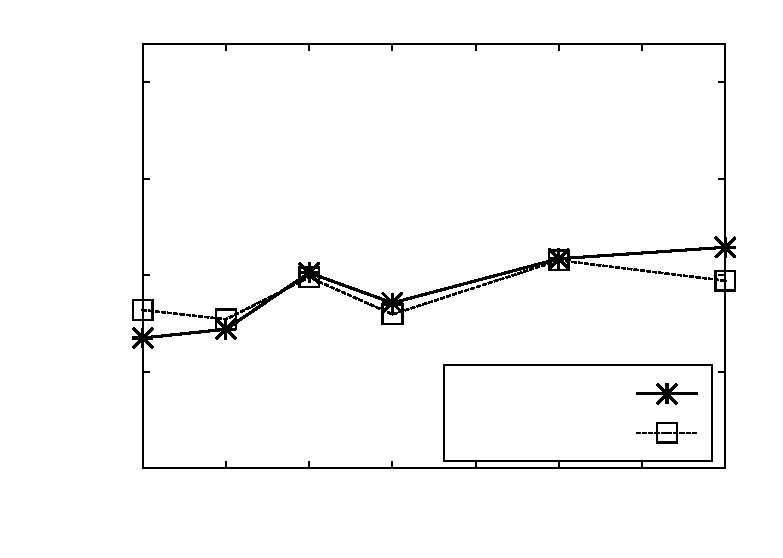
\includegraphics{graphs/database/b_read}}%
    \gplfronttext
  \end{picture}%
\endgroup
}} 
  \subfloat[][\textbf{Workload B:} update operations]{\resizebox{0.45\linewidth}{!}{% GNUPLOT: LaTeX picture with Postscript
\begingroup
  \makeatletter
  \providecommand\color[2][]{%
    \GenericError{(gnuplot) \space\space\space\@spaces}{%
      Package color not loaded in conjunction with
      terminal option `colourtext'%
    }{See the gnuplot documentation for explanation.%
    }{Either use 'blacktext' in gnuplot or load the package
      color.sty in LaTeX.}%
    \renewcommand\color[2][]{}%
  }%
  \providecommand\includegraphics[2][]{%
    \GenericError{(gnuplot) \space\space\space\@spaces}{%
      Package graphicx or graphics not loaded%
    }{See the gnuplot documentation for explanation.%
    }{The gnuplot epslatex terminal needs graphicx.sty or graphics.sty.}%
    \renewcommand\includegraphics[2][]{}%
  }%
  \providecommand\rotatebox[2]{#2}%
  \@ifundefined{ifGPcolor}{%
    \newif\ifGPcolor
    \GPcolorfalse
  }{}%
  \@ifundefined{ifGPblacktext}{%
    \newif\ifGPblacktext
    \GPblacktexttrue
  }{}%
  % define a \g@addto@macro without @ in the name:
  \let\gplgaddtomacro\g@addto@macro
  % define empty templates for all commands taking text:
  \gdef\gplbacktext{}%
  \gdef\gplfronttext{}%
  \makeatother
  \ifGPblacktext
    % no textcolor at all
    \def\colorrgb#1{}%
    \def\colorgray#1{}%
  \else
    % gray or color?
    \ifGPcolor
      \def\colorrgb#1{\color[rgb]{#1}}%
      \def\colorgray#1{\color[gray]{#1}}%
      \expandafter\def\csname LTw\endcsname{\color{white}}%
      \expandafter\def\csname LTb\endcsname{\color{black}}%
      \expandafter\def\csname LTa\endcsname{\color{black}}%
      \expandafter\def\csname LT0\endcsname{\color[rgb]{1,0,0}}%
      \expandafter\def\csname LT1\endcsname{\color[rgb]{0,1,0}}%
      \expandafter\def\csname LT2\endcsname{\color[rgb]{0,0,1}}%
      \expandafter\def\csname LT3\endcsname{\color[rgb]{1,0,1}}%
      \expandafter\def\csname LT4\endcsname{\color[rgb]{0,1,1}}%
      \expandafter\def\csname LT5\endcsname{\color[rgb]{1,1,0}}%
      \expandafter\def\csname LT6\endcsname{\color[rgb]{0,0,0}}%
      \expandafter\def\csname LT7\endcsname{\color[rgb]{1,0.3,0}}%
      \expandafter\def\csname LT8\endcsname{\color[rgb]{0.5,0.5,0.5}}%
    \else
      % gray
      \def\colorrgb#1{\color{black}}%
      \def\colorgray#1{\color[gray]{#1}}%
      \expandafter\def\csname LTw\endcsname{\color{white}}%
      \expandafter\def\csname LTb\endcsname{\color{black}}%
      \expandafter\def\csname LTa\endcsname{\color{black}}%
      \expandafter\def\csname LT0\endcsname{\color{black}}%
      \expandafter\def\csname LT1\endcsname{\color{black}}%
      \expandafter\def\csname LT2\endcsname{\color{black}}%
      \expandafter\def\csname LT3\endcsname{\color{black}}%
      \expandafter\def\csname LT4\endcsname{\color{black}}%
      \expandafter\def\csname LT5\endcsname{\color{black}}%
      \expandafter\def\csname LT6\endcsname{\color{black}}%
      \expandafter\def\csname LT7\endcsname{\color{black}}%
      \expandafter\def\csname LT8\endcsname{\color{black}}%
    \fi
  \fi
  \setlength{\unitlength}{0.0500bp}%
  \begin{picture}(7200.00,5040.00)%
    \gplgaddtomacro\gplbacktext{%
      \csname LTb\endcsname%
      \put(1078,704){\makebox(0,0)[r]{\strut{} 0}}%
      \put(1078,1629){\makebox(0,0)[r]{\strut{} 500}}%
      \put(1078,2554){\makebox(0,0)[r]{\strut{} 1000}}%
      \put(1078,3480){\makebox(0,0)[r]{\strut{} 1500}}%
      \put(1078,4405){\makebox(0,0)[r]{\strut{} 2000}}%
      \put(1210,484){\makebox(0,0){\strut{} 0}}%
      \put(1909,484){\makebox(0,0){\strut{} 5}}%
      \put(2608,484){\makebox(0,0){\strut{} 10}}%
      \put(3307,484){\makebox(0,0){\strut{} 15}}%
      \put(4007,484){\makebox(0,0){\strut{} 20}}%
      \put(4706,484){\makebox(0,0){\strut{} 25}}%
      \put(5405,484){\makebox(0,0){\strut{} 30}}%
      \put(6104,484){\makebox(0,0){\strut{} 35}}%
      \put(6803,484){\makebox(0,0){\strut{} 40}}%
      \put(176,2739){\rotatebox{-270}{\makebox(0,0){\strut{}Update latency (us)}}}%
      \put(4006,154){\makebox(0,0){\strut{}Throughput (thousand ops/sec)}}%
    }%
    \gplgaddtomacro\gplfronttext{%
      \csname LTb\endcsname%
      \put(5816,1416){\makebox(0,0)[r]{\strut{}Shuttle}}%
      \csname LTb\endcsname%
      \put(5816,1042){\makebox(0,0)[r]{\strut{}No Shuttle}}%
    }%
    \gplbacktext
    \put(0,0){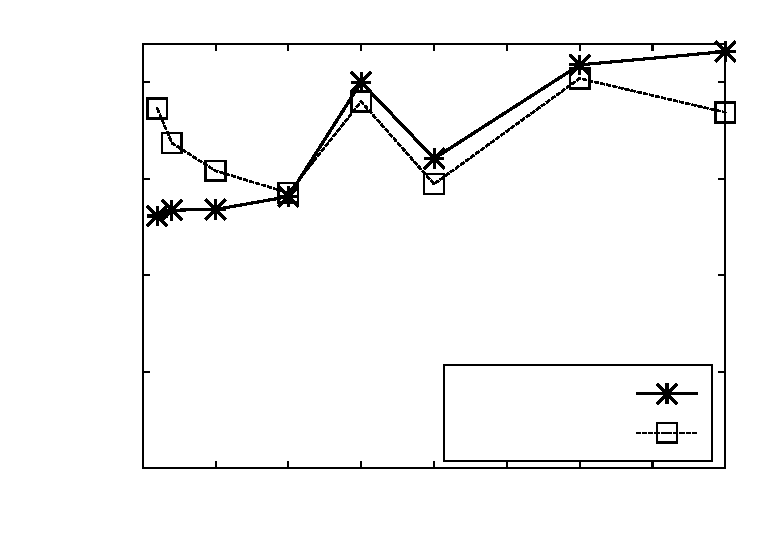
\includegraphics{graphs/database/b_update}}%
    \gplfronttext
  \end{picture}%
\endgroup
}}

  \subfloat[][\textbf{Workload C:} read operations]{\resizebox{0.45\linewidth}{!}{% GNUPLOT: LaTeX picture with Postscript
\begingroup
  \makeatletter
  \providecommand\color[2][]{%
    \GenericError{(gnuplot) \space\space\space\@spaces}{%
      Package color not loaded in conjunction with
      terminal option `colourtext'%
    }{See the gnuplot documentation for explanation.%
    }{Either use 'blacktext' in gnuplot or load the package
      color.sty in LaTeX.}%
    \renewcommand\color[2][]{}%
  }%
  \providecommand\includegraphics[2][]{%
    \GenericError{(gnuplot) \space\space\space\@spaces}{%
      Package graphicx or graphics not loaded%
    }{See the gnuplot documentation for explanation.%
    }{The gnuplot epslatex terminal needs graphicx.sty or graphics.sty.}%
    \renewcommand\includegraphics[2][]{}%
  }%
  \providecommand\rotatebox[2]{#2}%
  \@ifundefined{ifGPcolor}{%
    \newif\ifGPcolor
    \GPcolorfalse
  }{}%
  \@ifundefined{ifGPblacktext}{%
    \newif\ifGPblacktext
    \GPblacktexttrue
  }{}%
  % define a \g@addto@macro without @ in the name:
  \let\gplgaddtomacro\g@addto@macro
  % define empty templates for all commands taking text:
  \gdef\gplbacktext{}%
  \gdef\gplfronttext{}%
  \makeatother
  \ifGPblacktext
    % no textcolor at all
    \def\colorrgb#1{}%
    \def\colorgray#1{}%
  \else
    % gray or color?
    \ifGPcolor
      \def\colorrgb#1{\color[rgb]{#1}}%
      \def\colorgray#1{\color[gray]{#1}}%
      \expandafter\def\csname LTw\endcsname{\color{white}}%
      \expandafter\def\csname LTb\endcsname{\color{black}}%
      \expandafter\def\csname LTa\endcsname{\color{black}}%
      \expandafter\def\csname LT0\endcsname{\color[rgb]{1,0,0}}%
      \expandafter\def\csname LT1\endcsname{\color[rgb]{0,1,0}}%
      \expandafter\def\csname LT2\endcsname{\color[rgb]{0,0,1}}%
      \expandafter\def\csname LT3\endcsname{\color[rgb]{1,0,1}}%
      \expandafter\def\csname LT4\endcsname{\color[rgb]{0,1,1}}%
      \expandafter\def\csname LT5\endcsname{\color[rgb]{1,1,0}}%
      \expandafter\def\csname LT6\endcsname{\color[rgb]{0,0,0}}%
      \expandafter\def\csname LT7\endcsname{\color[rgb]{1,0.3,0}}%
      \expandafter\def\csname LT8\endcsname{\color[rgb]{0.5,0.5,0.5}}%
    \else
      % gray
      \def\colorrgb#1{\color{black}}%
      \def\colorgray#1{\color[gray]{#1}}%
      \expandafter\def\csname LTw\endcsname{\color{white}}%
      \expandafter\def\csname LTb\endcsname{\color{black}}%
      \expandafter\def\csname LTa\endcsname{\color{black}}%
      \expandafter\def\csname LT0\endcsname{\color{black}}%
      \expandafter\def\csname LT1\endcsname{\color{black}}%
      \expandafter\def\csname LT2\endcsname{\color{black}}%
      \expandafter\def\csname LT3\endcsname{\color{black}}%
      \expandafter\def\csname LT4\endcsname{\color{black}}%
      \expandafter\def\csname LT5\endcsname{\color{black}}%
      \expandafter\def\csname LT6\endcsname{\color{black}}%
      \expandafter\def\csname LT7\endcsname{\color{black}}%
      \expandafter\def\csname LT8\endcsname{\color{black}}%
    \fi
  \fi
  \setlength{\unitlength}{0.0500bp}%
  \begin{picture}(7200.00,5040.00)%
    \gplgaddtomacro\gplbacktext{%
      \csname LTb\endcsname%
      \put(1078,704){\makebox(0,0)[r]{\strut{} 0}}%
      \put(1078,1629){\makebox(0,0)[r]{\strut{} 500}}%
      \put(1078,2554){\makebox(0,0)[r]{\strut{} 1000}}%
      \put(1078,3480){\makebox(0,0)[r]{\strut{} 1500}}%
      \put(1078,4405){\makebox(0,0)[r]{\strut{} 2000}}%
      \put(1210,484){\makebox(0,0){\strut{} 0}}%
      \put(2142,484){\makebox(0,0){\strut{} 10}}%
      \put(3074,484){\makebox(0,0){\strut{} 20}}%
      \put(4007,484){\makebox(0,0){\strut{} 30}}%
      \put(4939,484){\makebox(0,0){\strut{} 40}}%
      \put(5871,484){\makebox(0,0){\strut{} 50}}%
      \put(6803,484){\makebox(0,0){\strut{} 60}}%
      \put(176,2739){\rotatebox{-270}{\makebox(0,0){\strut{}Read latency (us)}}}%
      \put(4006,154){\makebox(0,0){\strut{}Throughput (thousand ops/sec)}}%
    }%
    \gplgaddtomacro\gplfronttext{%
      \csname LTb\endcsname%
      \put(5816,1416){\makebox(0,0)[r]{\strut{}Shuttle}}%
      \csname LTb\endcsname%
      \put(5816,1042){\makebox(0,0)[r]{\strut{}No Shuttle}}%
    }%
    \gplbacktext
    \put(0,0){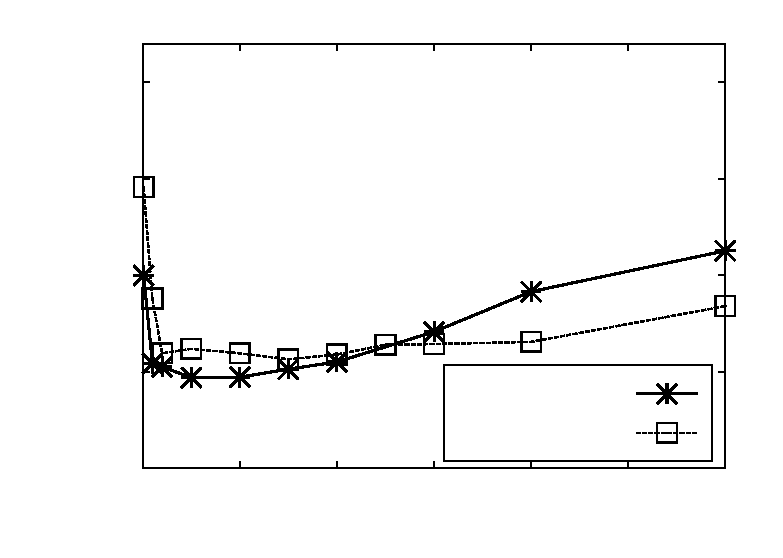
\includegraphics{graphs/database/c_read}}%
    \gplfronttext
  \end{picture}%
\endgroup
}} 

  \subfloat[][\textbf{Workload D:} read operations]{\resizebox{0.45\linewidth}{!}{% GNUPLOT: LaTeX picture with Postscript
\begingroup
  \makeatletter
  \providecommand\color[2][]{%
    \GenericError{(gnuplot) \space\space\space\@spaces}{%
      Package color not loaded in conjunction with
      terminal option `colourtext'%
    }{See the gnuplot documentation for explanation.%
    }{Either use 'blacktext' in gnuplot or load the package
      color.sty in LaTeX.}%
    \renewcommand\color[2][]{}%
  }%
  \providecommand\includegraphics[2][]{%
    \GenericError{(gnuplot) \space\space\space\@spaces}{%
      Package graphicx or graphics not loaded%
    }{See the gnuplot documentation for explanation.%
    }{The gnuplot epslatex terminal needs graphicx.sty or graphics.sty.}%
    \renewcommand\includegraphics[2][]{}%
  }%
  \providecommand\rotatebox[2]{#2}%
  \@ifundefined{ifGPcolor}{%
    \newif\ifGPcolor
    \GPcolorfalse
  }{}%
  \@ifundefined{ifGPblacktext}{%
    \newif\ifGPblacktext
    \GPblacktexttrue
  }{}%
  % define a \g@addto@macro without @ in the name:
  \let\gplgaddtomacro\g@addto@macro
  % define empty templates for all commands taking text:
  \gdef\gplbacktext{}%
  \gdef\gplfronttext{}%
  \makeatother
  \ifGPblacktext
    % no textcolor at all
    \def\colorrgb#1{}%
    \def\colorgray#1{}%
  \else
    % gray or color?
    \ifGPcolor
      \def\colorrgb#1{\color[rgb]{#1}}%
      \def\colorgray#1{\color[gray]{#1}}%
      \expandafter\def\csname LTw\endcsname{\color{white}}%
      \expandafter\def\csname LTb\endcsname{\color{black}}%
      \expandafter\def\csname LTa\endcsname{\color{black}}%
      \expandafter\def\csname LT0\endcsname{\color[rgb]{1,0,0}}%
      \expandafter\def\csname LT1\endcsname{\color[rgb]{0,1,0}}%
      \expandafter\def\csname LT2\endcsname{\color[rgb]{0,0,1}}%
      \expandafter\def\csname LT3\endcsname{\color[rgb]{1,0,1}}%
      \expandafter\def\csname LT4\endcsname{\color[rgb]{0,1,1}}%
      \expandafter\def\csname LT5\endcsname{\color[rgb]{1,1,0}}%
      \expandafter\def\csname LT6\endcsname{\color[rgb]{0,0,0}}%
      \expandafter\def\csname LT7\endcsname{\color[rgb]{1,0.3,0}}%
      \expandafter\def\csname LT8\endcsname{\color[rgb]{0.5,0.5,0.5}}%
    \else
      % gray
      \def\colorrgb#1{\color{black}}%
      \def\colorgray#1{\color[gray]{#1}}%
      \expandafter\def\csname LTw\endcsname{\color{white}}%
      \expandafter\def\csname LTb\endcsname{\color{black}}%
      \expandafter\def\csname LTa\endcsname{\color{black}}%
      \expandafter\def\csname LT0\endcsname{\color{black}}%
      \expandafter\def\csname LT1\endcsname{\color{black}}%
      \expandafter\def\csname LT2\endcsname{\color{black}}%
      \expandafter\def\csname LT3\endcsname{\color{black}}%
      \expandafter\def\csname LT4\endcsname{\color{black}}%
      \expandafter\def\csname LT5\endcsname{\color{black}}%
      \expandafter\def\csname LT6\endcsname{\color{black}}%
      \expandafter\def\csname LT7\endcsname{\color{black}}%
      \expandafter\def\csname LT8\endcsname{\color{black}}%
    \fi
  \fi
  \setlength{\unitlength}{0.0500bp}%
  \begin{picture}(7200.00,5040.00)%
    \gplgaddtomacro\gplbacktext{%
      \csname LTb\endcsname%
      \put(1078,704){\makebox(0,0)[r]{\strut{} 0}}%
      \put(1078,1629){\makebox(0,0)[r]{\strut{} 500}}%
      \put(1078,2554){\makebox(0,0)[r]{\strut{} 1000}}%
      \put(1078,3480){\makebox(0,0)[r]{\strut{} 1500}}%
      \put(1078,4405){\makebox(0,0)[r]{\strut{} 2000}}%
      \put(1210,484){\makebox(0,0){\strut{} 0}}%
      \put(1909,484){\makebox(0,0){\strut{} 5}}%
      \put(2608,484){\makebox(0,0){\strut{} 10}}%
      \put(3307,484){\makebox(0,0){\strut{} 15}}%
      \put(4007,484){\makebox(0,0){\strut{} 20}}%
      \put(4706,484){\makebox(0,0){\strut{} 25}}%
      \put(5405,484){\makebox(0,0){\strut{} 30}}%
      \put(6104,484){\makebox(0,0){\strut{} 35}}%
      \put(6803,484){\makebox(0,0){\strut{} 40}}%
      \put(176,2739){\rotatebox{-270}{\makebox(0,0){\strut{}Read latency (us)}}}%
      \put(4006,154){\makebox(0,0){\strut{}Throughput (thousand ops/sec)}}%
    }%
    \gplgaddtomacro\gplfronttext{%
      \csname LTb\endcsname%
      \put(5816,1416){\makebox(0,0)[r]{\strut{}Shuttle}}%
      \csname LTb\endcsname%
      \put(5816,1042){\makebox(0,0)[r]{\strut{}No Shuttle}}%
    }%
    \gplbacktext
    \put(0,0){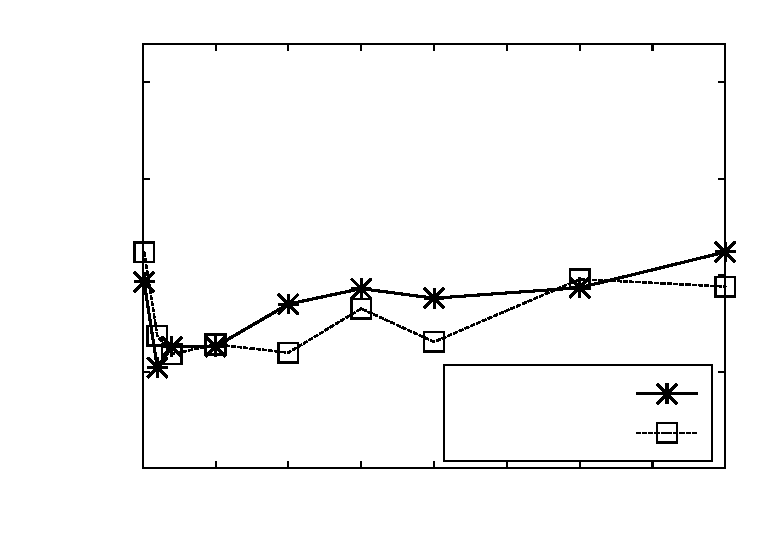
\includegraphics{graphs/database/d_read}}%
    \gplfronttext
  \end{picture}%
\endgroup
}} 
  \subfloat[][\textbf{Workload D:} insert operations]{\resizebox{0.45\linewidth}{!}{% GNUPLOT: LaTeX picture with Postscript
\begingroup
  \makeatletter
  \providecommand\color[2][]{%
    \GenericError{(gnuplot) \space\space\space\@spaces}{%
      Package color not loaded in conjunction with
      terminal option `colourtext'%
    }{See the gnuplot documentation for explanation.%
    }{Either use 'blacktext' in gnuplot or load the package
      color.sty in LaTeX.}%
    \renewcommand\color[2][]{}%
  }%
  \providecommand\includegraphics[2][]{%
    \GenericError{(gnuplot) \space\space\space\@spaces}{%
      Package graphicx or graphics not loaded%
    }{See the gnuplot documentation for explanation.%
    }{The gnuplot epslatex terminal needs graphicx.sty or graphics.sty.}%
    \renewcommand\includegraphics[2][]{}%
  }%
  \providecommand\rotatebox[2]{#2}%
  \@ifundefined{ifGPcolor}{%
    \newif\ifGPcolor
    \GPcolorfalse
  }{}%
  \@ifundefined{ifGPblacktext}{%
    \newif\ifGPblacktext
    \GPblacktexttrue
  }{}%
  % define a \g@addto@macro without @ in the name:
  \let\gplgaddtomacro\g@addto@macro
  % define empty templates for all commands taking text:
  \gdef\gplbacktext{}%
  \gdef\gplfronttext{}%
  \makeatother
  \ifGPblacktext
    % no textcolor at all
    \def\colorrgb#1{}%
    \def\colorgray#1{}%
  \else
    % gray or color?
    \ifGPcolor
      \def\colorrgb#1{\color[rgb]{#1}}%
      \def\colorgray#1{\color[gray]{#1}}%
      \expandafter\def\csname LTw\endcsname{\color{white}}%
      \expandafter\def\csname LTb\endcsname{\color{black}}%
      \expandafter\def\csname LTa\endcsname{\color{black}}%
      \expandafter\def\csname LT0\endcsname{\color[rgb]{1,0,0}}%
      \expandafter\def\csname LT1\endcsname{\color[rgb]{0,1,0}}%
      \expandafter\def\csname LT2\endcsname{\color[rgb]{0,0,1}}%
      \expandafter\def\csname LT3\endcsname{\color[rgb]{1,0,1}}%
      \expandafter\def\csname LT4\endcsname{\color[rgb]{0,1,1}}%
      \expandafter\def\csname LT5\endcsname{\color[rgb]{1,1,0}}%
      \expandafter\def\csname LT6\endcsname{\color[rgb]{0,0,0}}%
      \expandafter\def\csname LT7\endcsname{\color[rgb]{1,0.3,0}}%
      \expandafter\def\csname LT8\endcsname{\color[rgb]{0.5,0.5,0.5}}%
    \else
      % gray
      \def\colorrgb#1{\color{black}}%
      \def\colorgray#1{\color[gray]{#1}}%
      \expandafter\def\csname LTw\endcsname{\color{white}}%
      \expandafter\def\csname LTb\endcsname{\color{black}}%
      \expandafter\def\csname LTa\endcsname{\color{black}}%
      \expandafter\def\csname LT0\endcsname{\color{black}}%
      \expandafter\def\csname LT1\endcsname{\color{black}}%
      \expandafter\def\csname LT2\endcsname{\color{black}}%
      \expandafter\def\csname LT3\endcsname{\color{black}}%
      \expandafter\def\csname LT4\endcsname{\color{black}}%
      \expandafter\def\csname LT5\endcsname{\color{black}}%
      \expandafter\def\csname LT6\endcsname{\color{black}}%
      \expandafter\def\csname LT7\endcsname{\color{black}}%
      \expandafter\def\csname LT8\endcsname{\color{black}}%
    \fi
  \fi
  \setlength{\unitlength}{0.0500bp}%
  \begin{picture}(7200.00,5040.00)%
    \gplgaddtomacro\gplbacktext{%
      \csname LTb\endcsname%
      \put(1078,704){\makebox(0,0)[r]{\strut{} 0}}%
      \put(1078,1629){\makebox(0,0)[r]{\strut{} 500}}%
      \put(1078,2554){\makebox(0,0)[r]{\strut{} 1000}}%
      \put(1078,3480){\makebox(0,0)[r]{\strut{} 1500}}%
      \put(1078,4405){\makebox(0,0)[r]{\strut{} 2000}}%
      \put(1210,484){\makebox(0,0){\strut{} 0}}%
      \put(1909,484){\makebox(0,0){\strut{} 5}}%
      \put(2608,484){\makebox(0,0){\strut{} 10}}%
      \put(3307,484){\makebox(0,0){\strut{} 15}}%
      \put(4007,484){\makebox(0,0){\strut{} 20}}%
      \put(4706,484){\makebox(0,0){\strut{} 25}}%
      \put(5405,484){\makebox(0,0){\strut{} 30}}%
      \put(6104,484){\makebox(0,0){\strut{} 35}}%
      \put(6803,484){\makebox(0,0){\strut{} 40}}%
      \put(176,2739){\rotatebox{-270}{\makebox(0,0){\strut{}Insert latency (us)}}}%
      \put(4006,154){\makebox(0,0){\strut{}Throughput (thousand ops/sec)}}%
    }%
    \gplgaddtomacro\gplfronttext{%
      \csname LTb\endcsname%
      \put(5816,1416){\makebox(0,0)[r]{\strut{}Shuttle}}%
      \csname LTb\endcsname%
      \put(5816,1042){\makebox(0,0)[r]{\strut{}No Shuttle}}%
    }%
    \gplbacktext
    \put(0,0){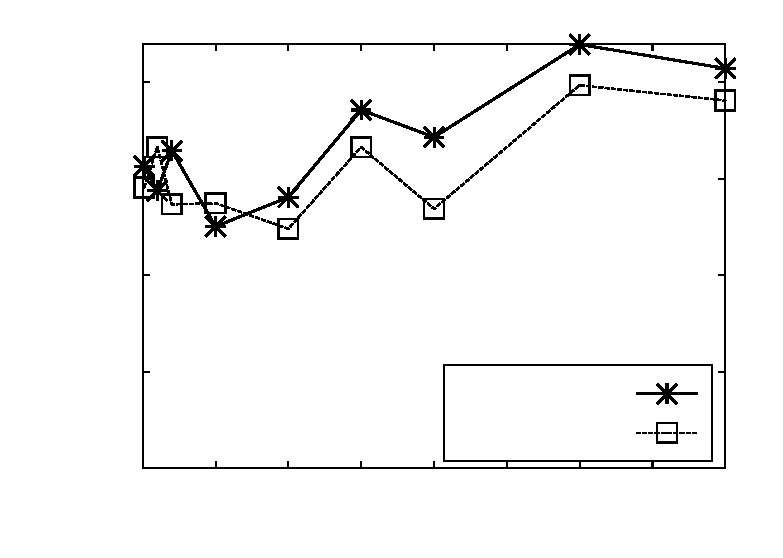
\includegraphics{graphs/database/d_insert}}%
    \gplfronttext
  \end{picture}%
\endgroup
}}
  \caption{Shuttle overhead on database}
  \label{fig:database_overhead_workloads}
\end{figure}

We expected the major Shuttle impact on database to be the read-write lock. Shuttle serializes the requests per-key using a read-write lock. In addition, the underlying \acf{BDB}, which is used by Voldemort as persistent-storage, also uses a read-write lock. However, the results in Figure \ref{fig:database_overhead_workloads} prove that Shuttle imposes a negligible latency overhead for the various types of workload and request rate.  

Shuttle also iterates over the \emph{operation lists} to determine the dependencies and sends them to the \emph{manager}. The instance's CPU usage was 10\% in average and the throughput did not reveal any variation when the dependencies are being collected. 

Shuttle snapshot mechanism requires creating a new data item in the Voldemort database and creating a new data version. A new version takes 264.077\us (standard deviation 864.293\us) to be created, while overwrite a version takes 266.635\us (std. deviation 577.124\us).

We conclude that Shuttle database proxy does not represent a significant performance overhead. %medi 1 milhao de entradas no meu computador


%---------------------------------- proxy ----------------------------------
\subsubsection{Proxy}\label{sec:eval:performance:proxy}
We setup an environment with 3 \ac{AWS} \textit{c3.xlarge} instances to measure the proxy overhead. The first runs a \ac{HTTP} benchmark tool \emph{weighttp} \cite{weighttp}. The second runs a HAProxy (v1.5.3) as load balancer and the Shuttle's proxy. The third runs a WildFly serving a 1KB static file. The benchmark tool performed 2 million requests using 8 threads and 200 clients.

\begin{figure}
  \begin{minipage}[t][][b]{0.55\linewidth}
    \resizebox{8cm}{!} {% GNUPLOT: LaTeX picture with Postscript
\begingroup
  \makeatletter
  \providecommand\color[2][]{%
    \GenericError{(gnuplot) \space\space\space\@spaces}{%
      Package color not loaded in conjunction with
      terminal option `colourtext'%
    }{See the gnuplot documentation for explanation.%
    }{Either use 'blacktext' in gnuplot or load the package
      color.sty in LaTeX.}%
    \renewcommand\color[2][]{}%
  }%
  \providecommand\includegraphics[2][]{%
    \GenericError{(gnuplot) \space\space\space\@spaces}{%
      Package graphicx or graphics not loaded%
    }{See the gnuplot documentation for explanation.%
    }{The gnuplot epslatex terminal needs graphicx.sty or graphics.sty.}%
    \renewcommand\includegraphics[2][]{}%
  }%
  \providecommand\rotatebox[2]{#2}%
  \@ifundefined{ifGPcolor}{%
    \newif\ifGPcolor
    \GPcolorfalse
  }{}%
  \@ifundefined{ifGPblacktext}{%
    \newif\ifGPblacktext
    \GPblacktexttrue
  }{}%
  % define a \g@addto@macro without @ in the name:
  \let\gplgaddtomacro\g@addto@macro
  % define empty templates for all commands taking text:
  \gdef\gplbacktext{}%
  \gdef\gplfronttext{}%
  \makeatother
  \ifGPblacktext
    % no textcolor at all
    \def\colorrgb#1{}%
    \def\colorgray#1{}%
  \else
    % gray or color?
    \ifGPcolor
      \def\colorrgb#1{\color[rgb]{#1}}%
      \def\colorgray#1{\color[gray]{#1}}%
      \expandafter\def\csname LTw\endcsname{\color{white}}%
      \expandafter\def\csname LTb\endcsname{\color{black}}%
      \expandafter\def\csname LTa\endcsname{\color{black}}%
      \expandafter\def\csname LT0\endcsname{\color[rgb]{1,0,0}}%
      \expandafter\def\csname LT1\endcsname{\color[rgb]{0,1,0}}%
      \expandafter\def\csname LT2\endcsname{\color[rgb]{0,0,1}}%
      \expandafter\def\csname LT3\endcsname{\color[rgb]{1,0,1}}%
      \expandafter\def\csname LT4\endcsname{\color[rgb]{0,1,1}}%
      \expandafter\def\csname LT5\endcsname{\color[rgb]{1,1,0}}%
      \expandafter\def\csname LT6\endcsname{\color[rgb]{0,0,0}}%
      \expandafter\def\csname LT7\endcsname{\color[rgb]{1,0.3,0}}%
      \expandafter\def\csname LT8\endcsname{\color[rgb]{0.5,0.5,0.5}}%
    \else
      % gray
      \def\colorrgb#1{\color{black}}%
      \def\colorgray#1{\color[gray]{#1}}%
      \expandafter\def\csname LTw\endcsname{\color{white}}%
      \expandafter\def\csname LTb\endcsname{\color{black}}%
      \expandafter\def\csname LTa\endcsname{\color{black}}%
      \expandafter\def\csname LT0\endcsname{\color{black}}%
      \expandafter\def\csname LT1\endcsname{\color{black}}%
      \expandafter\def\csname LT2\endcsname{\color{black}}%
      \expandafter\def\csname LT3\endcsname{\color{black}}%
      \expandafter\def\csname LT4\endcsname{\color{black}}%
      \expandafter\def\csname LT5\endcsname{\color{black}}%
      \expandafter\def\csname LT6\endcsname{\color{black}}%
      \expandafter\def\csname LT7\endcsname{\color{black}}%
      \expandafter\def\csname LT8\endcsname{\color{black}}%
    \fi
  \fi
  \setlength{\unitlength}{0.0500bp}%
  \begin{picture}(7200.00,5040.00)%
    \gplgaddtomacro\gplbacktext{%
      \csname LTb\endcsname%
      \put(1210,440){\makebox(0,0)[r]{\strut{} 0}}%
      \put(1210,1018){\makebox(0,0)[r]{\strut{} 10000}}%
      \put(1210,1596){\makebox(0,0)[r]{\strut{} 20000}}%
      \put(1210,2174){\makebox(0,0)[r]{\strut{} 30000}}%
      \put(1210,2752){\makebox(0,0)[r]{\strut{} 40000}}%
      \put(1210,3330){\makebox(0,0)[r]{\strut{} 50000}}%
      \put(1210,3908){\makebox(0,0)[r]{\strut{} 60000}}%
      \put(1210,4486){\makebox(0,0)[r]{\strut{} 70000}}%
      \put(1645,220){\makebox(0,0){\strut{}a}}%
      \put(2859,220){\makebox(0,0){\strut{}b}}%
      \put(4073,220){\makebox(0,0){\strut{}c}}%
      \put(5286,220){\makebox(0,0){\strut{}d}}%
      \put(6500,220){\makebox(0,0){\strut{}e}}%
      \put(176,2607){\rotatebox{-270}{\makebox(0,0){\strut{}Requests per second}}}%
    }%
    \gplgaddtomacro\gplfronttext{%
    }%
    \gplbacktext
    \put(0,0){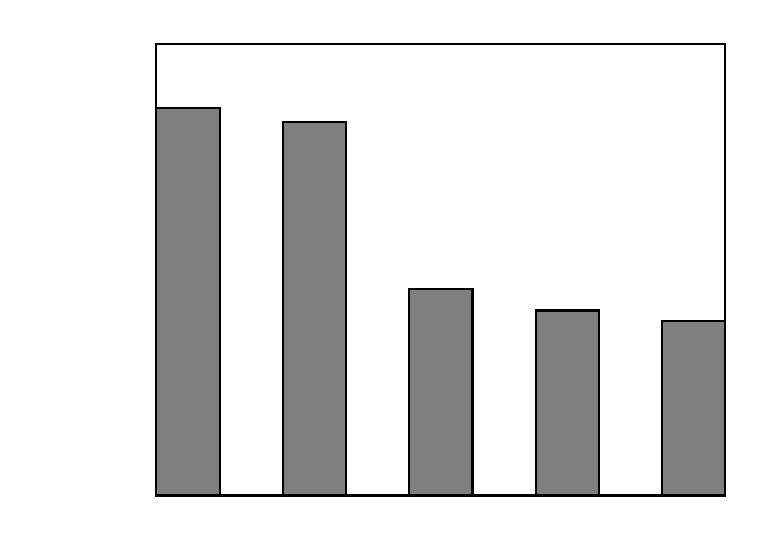
\includegraphics{graphs/proxy/throughput}}%
    \gplfronttext
  \end{picture}%
\endgroup
}
  \end{minipage}%
  \begin{minipage}[t][][b]{0.30\linewidth}
      \begin{tabular}{l|l|l|r}
            & \bf{Load Balancer} & \bf{Proxy}  & \bf{Latency (ms)}    \\ \hline
          a &                    &             & 1.08 (1.17)          \\
          b & \cmark             &             & 1.08 (1.25)          \\
          c &                    & \cmark      & 1.11 (1.28)          \\
          d & \cmark             & No log      & 1.10 (1.27)          \\
          e & \cmark             & \cmark      & 1.11 (1.29)          
      \end{tabular}
  \end{minipage}
\caption[Proxy Overhead]{Proxy Overhead: From left to right: direct to the server; only with the load balancer (HAProxy); Shuttle logging but without load balancer; overhead of Shuttle with load balancer when not logging and logging. The table describes the scenarios of the graph and the request latency (average and 95th percentile) in them. \hl{por favor, verifique a legenda. A tabela basicamente descreve o que o grafico tem e dá as latencias. É um bacoado manhoso}}
\label{fig:overhead_proxy}
\end{figure}

Figure \ref{fig:overhead_proxy} represents the throughput limit imposed by Shuttle's proxy. Shuttle's proxy imposes a considerable performance limitation (c) comparing with the load balancer (b). However, the logging mechanism has a negligible influence on the maximum request throughput (column \emph{d} comparing with column \emph{e}). In addition, the table in Figure \ref{fig:overhead_proxy} shows that Shuttle imposes a negligible overhead on requests latency considering a constant request income rate of 2500 requests per second. \hl{este parágrafo está bem escrito?}

We conclude that the performance overhead due to logging is negligible but the proxy is a considerable throughput limitation. The main cause is its implementation: while HAProxy is implemented using C and it is heavily optimized, Shuttle's proxy is a prototype implemented in Java. Therefore, we expect a C implementation of proxy can overcome the performance overhead. However, we claim that our prototype implementation is enough for most of small and enterprise services deployed in \ac{PaaS} because the throughput limit imposed by the proxy is lower than the request rates presented in Table \ref{tab:base_throughputs}. Moreover, the recovery time is dependent from the application performance but independent from the proxy's performance. \\  

%---------------------------------- webserver ----------------------------------
The overhead of Shuttle on each application server is database client interceptor that logs the accessed keys per request. Our experiments demonstrated that logging and storing the accessed keys implies a negligible overhead on the response latency.  \hl{este parágrafo fica um pouco deslocado certo? é só para não ter ficado nada por avaliar}


%---------------------------------- total ----------------------------------
\subsubsection{Total}\label{sec:eval:performance:total}
\hl{pois, total é uma marca de produtos petroquimicos. Eu não consegui arranjar um nome. Até aqui temos estado a ver parte a parte qual o overhead, aqui é do sistema completo, com tudo a funcionar}
We evaluate the overhead of Shuttle by measuring the throughput of the \textit{Ask} application with and without Shuttle (Table \ref{tab:throughput}). We do not consider a particular scenario or replay scheme (full/selective) but define instead the number of requests recovered per experiment. We run 6 \ac{AWS} \textit{c3.xlarge} instances. We use one client, one instance with Shuttle proxy and a load balancer (HAProxy), three WildFly application servers and one Voldemort database.

We considered two workloads: (A) has 50\% reads, 50\% inserts and (B) has 95\% reads, 5\% inserts. Insert operations adds questions, answers, comments and votes of the data sample, while read operations access the latest inserted questions. The insert operations insert the questions, answers, comments and votes of the data sample, while the read operations access the latest inserted questions. We consider a large data sample from \textit{StackExchange Data Dump} \cite{stackexchange_data} with 3 million requests (250812 questions, 335312 answers, 717937 comments, 1695939 votes).

Table \ref{tab:throughput} shows that Shuttle imposes an overhead of 13-20\%, which seems reasonable considering the benefits of having it. We believe the main cause of overhead is the current proxy, which is not very optimized. The current version written in Java performs considerably better than a previous version in Python, but we expect to be able to do much better by rewriting it in C. Still, while the proxy and database instances consume a low level of resources, the application instances consumed the maximum of CPU resources available.


\begin{table}
\centering
\begin{tabular}{l|rr}
                           &  \textbf{Workload A}   & \textbf{Workload B}  \\ \hline
\textbf{Shuttle}           &  6325 ops/sec [5.78 ms]  &  15346 ops/sec[3.62 ms]  \\
\textbf{No Shuttle}        &  7148 ops/sec [5.07 ms]  &  17821 ops/sec[3.01 ms]  \\
\end{tabular}
\caption{Shuttle overhead in terms of application throughput (ops/sec) and response latency (ms)}
\label{tab:throughput}
\end{table}

Considering the request rates presented in Table \ref{tab:base_throughputs}, we claim that a small environment with 6 machines is enough to support a small to medium application running with Shuttle. 

In conclusion, we prove that a single proxy architecture, which simplifies the Shuttle design by globally order the requests, is adequate. 




%%%%%%%%%%%%%%%%%%%%%%%%%%%%%%%%%%%%%%%%%%%%%%%%%%%%%%%%%%%%%%%%%%%%%%%%%%%%%%%%%%%%%%%%%%%%%%%%%%%%%%%%%%%%%%%%%%%%%%%%%%%%%%%%%%%%%%%


\subsection{Recovery}\label{sec:eval:recovery}
We measured the performance of the recovery process. We do not consider a particular scenario or replay scheme (full/selective) but define instead the number of requests recovered per experiment.

The recovery process can be summarized in the following points:

\begin{itemize}
  \item Generate the list of requests to replay;
  \item Launch replay instances; Launch new application servers and database instances, if instance rejuvenation is used;
  \item Replay the requests.
\end{itemize}

The main factors of influence on recovery performance are: 1) the number of requests to replay, which depends on the request arrival rate; 2) the detection delay; 3) the number and type of database operations of each request.


We setup a test environment with 6 \emph{c3.xlarge} instances in an \ac{AWS} \acf{VPC}, sharing the same placement group (Figure \ref{fig:aws_diagram}). The first instance runs the \emph{TryOut} testing application. The second runs Shuttle's manager, replay and Shuttle Storage (Cassandra). The third contains the application server WildFly with the application \emph{Ask}. The last instance runs the database.

\begin{figure}[!htb]
  \centering
  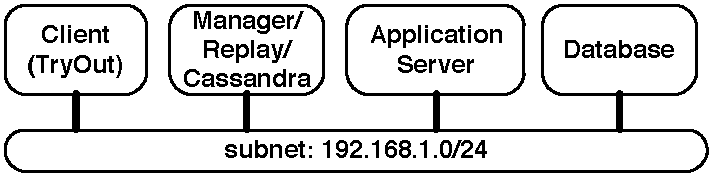
\includegraphics[width=90mm]{images/aws_diagram}
  \caption{Instances deployed on \ac{AWS} }
  \label{fig:aws_diagram}
\end{figure}


We considered a workload of 95\% reads, 5\% inserts (StackExchange network has a read/write ratio of 98.82\%). We consider a subset of \textit{StackExchange Data Dump} \cite{stackexchange_data} with 50 000 insert request (1432 questions, 3399 answers, 8335 comments, 36834 votes). Therefore, we consider a total of 1 million requests. The selected questions had 899 407 views in StackExchange. We consider 950 000 view requests. 

TryOut performed the 1 million requests in 672 seconds on average (1486 requests/second, standard deviation of 20 seconds) using 25 concurrent threads (Figure \ref{fig:recovery_period}). The average response latency was 15.82\ms (90th percentile of 22.826\ms and 95th of 27.721\ms). The resultant dependency graph has 1 million entries that establish 9 425 579 dependencies.\\



\subsubsection{Graph}\label{sec:eval:recovery:graph}
%---------------------------- Graph overhead --------------------------------------------
The list of requests to replay is generated using the dependency graph. A \emph{c3.xlarge} instance can insert 1 million requests, each depending from other 10 requests, in the graph in 6 seconds (166 000 requests per second). If each request depends on 2 other requests, then the same process takes 2 seconds. Each new request is represented as a novel entry in a Hash Table and each dependency requires modifying other entry (as the graph implementation is undirected). For web-scale applications, the dependency graph shall be implemented on a distributed hash table because of the graph storage requirements.\\


%sorting the execution list
The period to generate the execution list is defined by the time to sort the keys of the dependency graph hash table and copy the list. We sort the keys using Java's sorting algorithm, dual-Pivot Quicksort, which has a asymptotic complexity of \O{n \log{} n} for most of the data sets. On serial replay mode, the algorithm takes 150\ms (standard deviation of 31ms) to sort a dependency graph with 1 million entries and 279\ms (standard deviation of 24ms) to copy the sorted list. On clustered replay mode, the clustering algorithm takes on average 2218 \ms (standard deviation of 1869\ms) to determine the 1432 independent clusters of the graph. Then, it takes 533\ms (std. dev. of 165\ms) to sort the clusters and copy the list. %\hl{deveria ter explorado qual complexidade com que estes tempos crescem mas é dificil de dar garantias}  \hl{To determine the dependencies of selective replay takes....  o tempo que demora a achar as dependencias de selective replay é relevante? depende do numero de entradas tainted, da sua localizacao no grafo, das dependencias e da localizacao do snapshot}\\



\subsubsection{Instance Rejuvenation}\label{sec:eval:recovery:rejunation}
%---------------------------------- Image-recovery delay ----------------------------------
The time elapsed to launch a novel \emph{c3.xlarge} instance in \ac{AWS} depends on the current load of EC2. We measured 25 launches. The average time elapsed is 25 seconds (95th percentile of 40 sec) \hl{não :( não encontro onde é que deixei os valores das samples :(}. The time to deploy and launch the application depends on the application itself. The \emph{Ask} application is launched in less than 1 minute. The process is done by the \ac{PaaS} controller. We consider these delays negligible comparing with the total recovery period.\\

  
\subsubsection{Request Replay}\label{sec:eval:recovery:replay}
%---------------------------------- Recovery ----------------------------------
We performed full-replay considering a single-cluster of 1 million requests in 30 minutes (1717s or 584 requests per second) (Figure \ref{fig:recovery_period}). The average request rate is 726 requests per second (std. dev. 72). %\hl{ou seja, a amostra da figura faz a 584 mas a media e 726}. 

The performance is improved when considering 1432 independent clusters: 9 minutes (544s or 1795 requests per second) (Figure \ref{fig:recovery_period}). Despite the fact that independent clusters can be replayed concurrently, we consider the maximum of 30 clusters being replayed concurrently. The average throughput is 1966 requests per second (std. dev 224).

%discuss
The serial replay mode is not capable of fully exploring the application servers. While the first execution is performed using 25 client-threads and clustered replay using 30 client-threads, the serial replays uses one client-thread. We expect to solve this performance issue on future implementations. 
    
\begin{figure*}[!htb] 
    \centering
    \resizebox{0.7\linewidth}{!}{% GNUPLOT: LaTeX picture with Postscript
\begingroup
  \makeatletter
  \providecommand\color[2][]{%
    \GenericError{(gnuplot) \space\space\space\@spaces}{%
      Package color not loaded in conjunction with
      terminal option `colourtext'%
    }{See the gnuplot documentation for explanation.%
    }{Either use 'blacktext' in gnuplot or load the package
      color.sty in LaTeX.}%
    \renewcommand\color[2][]{}%
  }%
  \providecommand\includegraphics[2][]{%
    \GenericError{(gnuplot) \space\space\space\@spaces}{%
      Package graphicx or graphics not loaded%
    }{See the gnuplot documentation for explanation.%
    }{The gnuplot epslatex terminal needs graphicx.sty or graphics.sty.}%
    \renewcommand\includegraphics[2][]{}%
  }%
  \providecommand\rotatebox[2]{#2}%
  \@ifundefined{ifGPcolor}{%
    \newif\ifGPcolor
    \GPcolorfalse
  }{}%
  \@ifundefined{ifGPblacktext}{%
    \newif\ifGPblacktext
    \GPblacktexttrue
  }{}%
  % define a \g@addto@macro without @ in the name:
  \let\gplgaddtomacro\g@addto@macro
  % define empty templates for all commands taking text:
  \gdef\gplbacktext{}%
  \gdef\gplfronttext{}%
  \makeatother
  \ifGPblacktext
    % no textcolor at all
    \def\colorrgb#1{}%
    \def\colorgray#1{}%
  \else
    % gray or color?
    \ifGPcolor
      \def\colorrgb#1{\color[rgb]{#1}}%
      \def\colorgray#1{\color[gray]{#1}}%
      \expandafter\def\csname LTw\endcsname{\color{white}}%
      \expandafter\def\csname LTb\endcsname{\color{black}}%
      \expandafter\def\csname LTa\endcsname{\color{black}}%
      \expandafter\def\csname LT0\endcsname{\color[rgb]{1,0,0}}%
      \expandafter\def\csname LT1\endcsname{\color[rgb]{0,1,0}}%
      \expandafter\def\csname LT2\endcsname{\color[rgb]{0,0,1}}%
      \expandafter\def\csname LT3\endcsname{\color[rgb]{1,0,1}}%
      \expandafter\def\csname LT4\endcsname{\color[rgb]{0,1,1}}%
      \expandafter\def\csname LT5\endcsname{\color[rgb]{1,1,0}}%
      \expandafter\def\csname LT6\endcsname{\color[rgb]{0,0,0}}%
      \expandafter\def\csname LT7\endcsname{\color[rgb]{1,0.3,0}}%
      \expandafter\def\csname LT8\endcsname{\color[rgb]{0.5,0.5,0.5}}%
    \else
      % gray
      \def\colorrgb#1{\color{black}}%
      \def\colorgray#1{\color[gray]{#1}}%
      \expandafter\def\csname LTw\endcsname{\color{white}}%
      \expandafter\def\csname LTb\endcsname{\color{black}}%
      \expandafter\def\csname LTa\endcsname{\color{black}}%
      \expandafter\def\csname LT0\endcsname{\color{black}}%
      \expandafter\def\csname LT1\endcsname{\color{black}}%
      \expandafter\def\csname LT2\endcsname{\color{black}}%
      \expandafter\def\csname LT3\endcsname{\color{black}}%
      \expandafter\def\csname LT4\endcsname{\color{black}}%
      \expandafter\def\csname LT5\endcsname{\color{black}}%
      \expandafter\def\csname LT6\endcsname{\color{black}}%
      \expandafter\def\csname LT7\endcsname{\color{black}}%
      \expandafter\def\csname LT8\endcsname{\color{black}}%
    \fi
  \fi
  \setlength{\unitlength}{0.0500bp}%
  \begin{picture}(7200.00,5040.00)%
    \gplgaddtomacro\gplbacktext{%
      \csname LTb\endcsname%
      \put(1078,704){\makebox(0,0)[r]{\strut{} 20}}%
      \put(1078,1518){\makebox(0,0)[r]{\strut{} 20.2}}%
      \put(1078,2332){\makebox(0,0)[r]{\strut{} 20.4}}%
      \put(1078,3147){\makebox(0,0)[r]{\strut{} 20.6}}%
      \put(1078,3961){\makebox(0,0)[r]{\strut{} 20.8}}%
      \put(1078,4775){\makebox(0,0)[r]{\strut{} 21}}%
      \put(1210,484){\makebox(0,0){\strut{} 0}}%
      \put(2142,484){\makebox(0,0){\strut{} 2}}%
      \put(3074,484){\makebox(0,0){\strut{} 4}}%
      \put(4007,484){\makebox(0,0){\strut{} 6}}%
      \put(4939,484){\makebox(0,0){\strut{} 8}}%
      \put(5871,484){\makebox(0,0){\strut{} 10}}%
      \put(6803,484){\makebox(0,0){\strut{} 12}}%
      \put(176,2739){\rotatebox{-270}{\makebox(0,0){\strut{}Recovery time (ms)}}}%
      \put(4006,154){\makebox(0,0){\strut{}Number of requests}}%
    }%
    \gplgaddtomacro\gplfronttext{%
      \csname LTb\endcsname%
      \put(5816,4602){\makebox(0,0)[r]{\strut{}1 Cluster}}%
      \csname LTb\endcsname%
      \put(5816,4382){\makebox(0,0)[r]{\strut{}2 Clusters}}%
      \csname LTb\endcsname%
      \put(5816,4162){\makebox(0,0)[r]{\strut{}3 Cluster}}%
      \csname LTb\endcsname%
      \put(5816,3942){\makebox(0,0)[r]{\strut{}4 Clusters}}%
      \csname LTb\endcsname%
      \put(5816,3722){\makebox(0,0)[r]{\strut{}5 Clusters}}%
    }%
    \gplbacktext
    \put(0,0){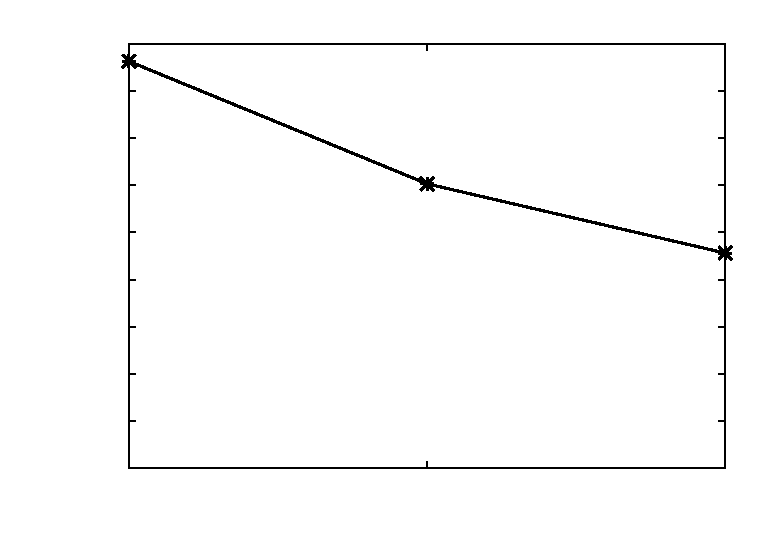
\includegraphics{graphs/clusters/grafico}}%
    \gplfronttext
  \end{picture}%
\endgroup
}
    \caption{Recovery period without new incoming requests}
    \label{fig:recovery_period}
\end{figure*}




\subsubsection{Restrain}\label{sec:eval:recovery:restrain}
%--------------------------------- Restrain --------------------------------- ---
%serial
We measured the duration of the restrain period considering two clients with a constant throughput of 400 requests/sec (Figure \ref{fig:restrain:serial}). 

Considering serial replay, the average response time of new incoming requests is 3.94\ms (95th percentile of 10.34\ms, 90th of 7.53\ms). Since the serial replay mode is not capable of fully exploring the application servers, the new incoming requests are not affected by the replay process. The replay process takes on average 30 minutes (1850\ms). Since the Shuttle takes 30 minutes to replay 1 million requests, the new flow generates 298 thousand new requests. Shuttle takes 18 minutes to replay these new requests. The user requests are suspended until the new requests are replayed and the branch is changed. This delay is considerable because the throughput of new requests is close to the throughput of the requests being replayed. The delay can be reduced by replaying the new requests and then block to replay the newer requests, i.e., creating several phases of replay. fazer varias fases, cada vez mais curtas porque vai compensando a diferenca. In addition, if the replay rate is bigger than the rate of new incoming requests, then the restrain phase is shorter.\\
%The serial replay mode is not capable of fully exploring the application servers so it takes almost one hour to recover (2953s total, 1100s in restrain mode) (Figure \ref{fig:restrain:serial})

%parallel
If Shuttle performs clustered replay, the application servers are overloaded. Consequently, the average response time of new incoming requests is 5.51\ms (95th percentile of 13.56\ms, 90th of 10.60\ms) and the throughput of the new incoming requests drops from 200 to 95 requests per second. On other hand, the throughput of requests being replayed drops from 1795 to 1686 req./sec. The recovery process takes a total 10 minutes (635 seconds). Therefore, the customers perform 56 000 requests. These requests are replayed in 46 seconds (Figure \ref{fig:restrain:clustered}). 



    
\begin{figure*}[!htb] 
    \centering
    \resizebox{0.7\linewidth}{!}{% GNUPLOT: LaTeX picture with Postscript
\begingroup
  \makeatletter
  \providecommand\color[2][]{%
    \GenericError{(gnuplot) \space\space\space\@spaces}{%
      Package color not loaded in conjunction with
      terminal option `colourtext'%
    }{See the gnuplot documentation for explanation.%
    }{Either use 'blacktext' in gnuplot or load the package
      color.sty in LaTeX.}%
    \renewcommand\color[2][]{}%
  }%
  \providecommand\includegraphics[2][]{%
    \GenericError{(gnuplot) \space\space\space\@spaces}{%
      Package graphicx or graphics not loaded%
    }{See the gnuplot documentation for explanation.%
    }{The gnuplot epslatex terminal needs graphicx.sty or graphics.sty.}%
    \renewcommand\includegraphics[2][]{}%
  }%
  \providecommand\rotatebox[2]{#2}%
  \@ifundefined{ifGPcolor}{%
    \newif\ifGPcolor
    \GPcolorfalse
  }{}%
  \@ifundefined{ifGPblacktext}{%
    \newif\ifGPblacktext
    \GPblacktexttrue
  }{}%
  % define a \g@addto@macro without @ in the name:
  \let\gplgaddtomacro\g@addto@macro
  % define empty templates for all commands taking text:
  \gdef\gplbacktext{}%
  \gdef\gplfronttext{}%
  \makeatother
  \ifGPblacktext
    % no textcolor at all
    \def\colorrgb#1{}%
    \def\colorgray#1{}%
  \else
    % gray or color?
    \ifGPcolor
      \def\colorrgb#1{\color[rgb]{#1}}%
      \def\colorgray#1{\color[gray]{#1}}%
      \expandafter\def\csname LTw\endcsname{\color{white}}%
      \expandafter\def\csname LTb\endcsname{\color{black}}%
      \expandafter\def\csname LTa\endcsname{\color{black}}%
      \expandafter\def\csname LT0\endcsname{\color[rgb]{1,0,0}}%
      \expandafter\def\csname LT1\endcsname{\color[rgb]{0,1,0}}%
      \expandafter\def\csname LT2\endcsname{\color[rgb]{0,0,1}}%
      \expandafter\def\csname LT3\endcsname{\color[rgb]{1,0,1}}%
      \expandafter\def\csname LT4\endcsname{\color[rgb]{0,1,1}}%
      \expandafter\def\csname LT5\endcsname{\color[rgb]{1,1,0}}%
      \expandafter\def\csname LT6\endcsname{\color[rgb]{0,0,0}}%
      \expandafter\def\csname LT7\endcsname{\color[rgb]{1,0.3,0}}%
      \expandafter\def\csname LT8\endcsname{\color[rgb]{0.5,0.5,0.5}}%
    \else
      % gray
      \def\colorrgb#1{\color{black}}%
      \def\colorgray#1{\color[gray]{#1}}%
      \expandafter\def\csname LTw\endcsname{\color{white}}%
      \expandafter\def\csname LTb\endcsname{\color{black}}%
      \expandafter\def\csname LTa\endcsname{\color{black}}%
      \expandafter\def\csname LT0\endcsname{\color{black}}%
      \expandafter\def\csname LT1\endcsname{\color{black}}%
      \expandafter\def\csname LT2\endcsname{\color{black}}%
      \expandafter\def\csname LT3\endcsname{\color{black}}%
      \expandafter\def\csname LT4\endcsname{\color{black}}%
      \expandafter\def\csname LT5\endcsname{\color{black}}%
      \expandafter\def\csname LT6\endcsname{\color{black}}%
      \expandafter\def\csname LT7\endcsname{\color{black}}%
      \expandafter\def\csname LT8\endcsname{\color{black}}%
    \fi
  \fi
  \setlength{\unitlength}{0.0500bp}%
  \begin{picture}(7200.00,5040.00)%
    \gplgaddtomacro\gplbacktext{%
      \csname LTb\endcsname%
      \put(1078,704){\makebox(0,0)[r]{\strut{} 0}}%
      \put(1078,1383){\makebox(0,0)[r]{\strut{} 500}}%
      \put(1078,2061){\makebox(0,0)[r]{\strut{} 1000}}%
      \put(1078,2740){\makebox(0,0)[r]{\strut{} 1500}}%
      \put(1078,3418){\makebox(0,0)[r]{\strut{} 2000}}%
      \put(1078,4097){\makebox(0,0)[r]{\strut{} 2500}}%
      \put(1078,4775){\makebox(0,0)[r]{\strut{} 3000}}%
      \put(1210,484){\makebox(0,0){\strut{}00:00}}%
      \put(1778,484){\makebox(0,0){\strut{}05:00}}%
      \put(2346,484){\makebox(0,0){\strut{}10:00}}%
      \put(2915,484){\makebox(0,0){\strut{}15:00}}%
      \put(3483,484){\makebox(0,0){\strut{}20:00}}%
      \put(4051,484){\makebox(0,0){\strut{}25:00}}%
      \put(4619,484){\makebox(0,0){\strut{}30:00}}%
      \put(5187,484){\makebox(0,0){\strut{}35:00}}%
      \put(5756,484){\makebox(0,0){\strut{}40:00}}%
      \put(6324,484){\makebox(0,0){\strut{}45:00}}%
      \put(176,2739){\rotatebox{-270}{\makebox(0,0){\strut{}Requests per second}}}%
      \put(4006,154){\makebox(0,0){\strut{}Time (minutes:seconds)}}%
      \put(4714,3418){\makebox(0,0)[l]{\strut{}Restrain}}%
    }%
    \gplgaddtomacro\gplfronttext{%
      \csname LTb\endcsname%
      \put(5816,4481){\makebox(0,0)[r]{\strut{}serial replay}}%
      \csname LTb\endcsname%
      \put(5816,4195){\makebox(0,0)[r]{\strut{}concurrent client}}%
    }%
    \gplbacktext
    \put(0,0){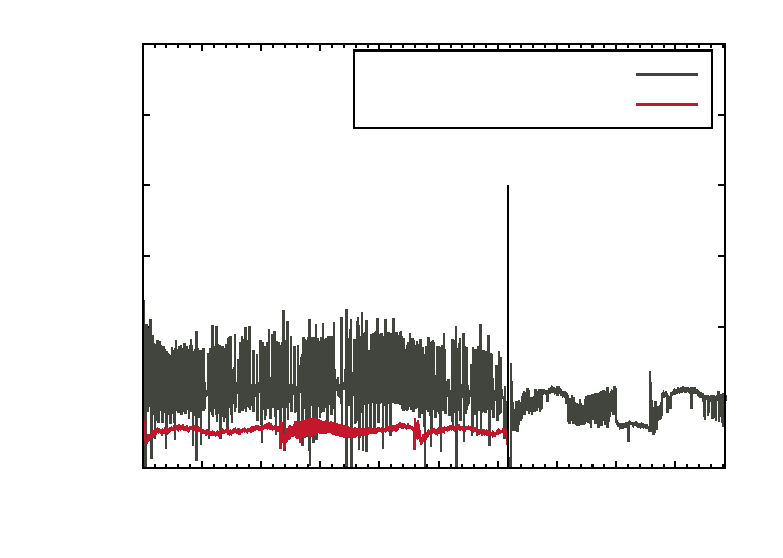
\includegraphics{graphs/restrain/serial_restrain}}%
    \gplfronttext
  \end{picture}%
\endgroup
}
    \caption{Serial Recovery: Requests throughput during the recovery period}
    \label{fig:restrain:serial}
\end{figure*}
    
\begin{figure*}[!htb] 
    \centering
    \resizebox{0.7\linewidth}{!}{% GNUPLOT: LaTeX picture with Postscript
\begingroup
  \makeatletter
  \providecommand\color[2][]{%
    \GenericError{(gnuplot) \space\space\space\@spaces}{%
      Package color not loaded in conjunction with
      terminal option `colourtext'%
    }{See the gnuplot documentation for explanation.%
    }{Either use 'blacktext' in gnuplot or load the package
      color.sty in LaTeX.}%
    \renewcommand\color[2][]{}%
  }%
  \providecommand\includegraphics[2][]{%
    \GenericError{(gnuplot) \space\space\space\@spaces}{%
      Package graphicx or graphics not loaded%
    }{See the gnuplot documentation for explanation.%
    }{The gnuplot epslatex terminal needs graphicx.sty or graphics.sty.}%
    \renewcommand\includegraphics[2][]{}%
  }%
  \providecommand\rotatebox[2]{#2}%
  \@ifundefined{ifGPcolor}{%
    \newif\ifGPcolor
    \GPcolorfalse
  }{}%
  \@ifundefined{ifGPblacktext}{%
    \newif\ifGPblacktext
    \GPblacktexttrue
  }{}%
  % define a \g@addto@macro without @ in the name:
  \let\gplgaddtomacro\g@addto@macro
  % define empty templates for all commands taking text:
  \gdef\gplbacktext{}%
  \gdef\gplfronttext{}%
  \makeatother
  \ifGPblacktext
    % no textcolor at all
    \def\colorrgb#1{}%
    \def\colorgray#1{}%
  \else
    % gray or color?
    \ifGPcolor
      \def\colorrgb#1{\color[rgb]{#1}}%
      \def\colorgray#1{\color[gray]{#1}}%
      \expandafter\def\csname LTw\endcsname{\color{white}}%
      \expandafter\def\csname LTb\endcsname{\color{black}}%
      \expandafter\def\csname LTa\endcsname{\color{black}}%
      \expandafter\def\csname LT0\endcsname{\color[rgb]{1,0,0}}%
      \expandafter\def\csname LT1\endcsname{\color[rgb]{0,1,0}}%
      \expandafter\def\csname LT2\endcsname{\color[rgb]{0,0,1}}%
      \expandafter\def\csname LT3\endcsname{\color[rgb]{1,0,1}}%
      \expandafter\def\csname LT4\endcsname{\color[rgb]{0,1,1}}%
      \expandafter\def\csname LT5\endcsname{\color[rgb]{1,1,0}}%
      \expandafter\def\csname LT6\endcsname{\color[rgb]{0,0,0}}%
      \expandafter\def\csname LT7\endcsname{\color[rgb]{1,0.3,0}}%
      \expandafter\def\csname LT8\endcsname{\color[rgb]{0.5,0.5,0.5}}%
    \else
      % gray
      \def\colorrgb#1{\color{black}}%
      \def\colorgray#1{\color[gray]{#1}}%
      \expandafter\def\csname LTw\endcsname{\color{white}}%
      \expandafter\def\csname LTb\endcsname{\color{black}}%
      \expandafter\def\csname LTa\endcsname{\color{black}}%
      \expandafter\def\csname LT0\endcsname{\color{black}}%
      \expandafter\def\csname LT1\endcsname{\color{black}}%
      \expandafter\def\csname LT2\endcsname{\color{black}}%
      \expandafter\def\csname LT3\endcsname{\color{black}}%
      \expandafter\def\csname LT4\endcsname{\color{black}}%
      \expandafter\def\csname LT5\endcsname{\color{black}}%
      \expandafter\def\csname LT6\endcsname{\color{black}}%
      \expandafter\def\csname LT7\endcsname{\color{black}}%
      \expandafter\def\csname LT8\endcsname{\color{black}}%
    \fi
  \fi
  \setlength{\unitlength}{0.0500bp}%
  \begin{picture}(7200.00,5040.00)%
    \gplgaddtomacro\gplbacktext{%
      \csname LTb\endcsname%
      \put(1078,704){\makebox(0,0)[r]{\strut{} 0}}%
      \put(1078,1383){\makebox(0,0)[r]{\strut{} 500}}%
      \put(1078,2061){\makebox(0,0)[r]{\strut{} 1000}}%
      \put(1078,2740){\makebox(0,0)[r]{\strut{} 1500}}%
      \put(1078,3418){\makebox(0,0)[r]{\strut{} 2000}}%
      \put(1078,4097){\makebox(0,0)[r]{\strut{} 2500}}%
      \put(1078,4775){\makebox(0,0)[r]{\strut{} 3000}}%
      \put(1210,484){\makebox(0,0){\strut{}00:00}}%
      \put(2267,484){\makebox(0,0){\strut{}02:00}}%
      \put(3324,484){\makebox(0,0){\strut{}04:00}}%
      \put(4381,484){\makebox(0,0){\strut{}06:00}}%
      \put(5438,484){\makebox(0,0){\strut{}08:00}}%
      \put(6495,484){\makebox(0,0){\strut{}10:00}}%
      \put(176,2739){\rotatebox{-270}{\makebox(0,0){\strut{}Requests per second}}}%
      \put(4006,154){\makebox(0,0){\strut{}Time (minutes:seconds)}}%
      \put(17505,3418){\makebox(0,0)[l]{\strut{}Restrain}}%
    }%
    \gplgaddtomacro\gplfronttext{%
      \csname LTb\endcsname%
      \put(5816,4481){\makebox(0,0)[r]{\strut{}clustered replay}}%
      \csname LTb\endcsname%
      \put(5816,4195){\makebox(0,0)[r]{\strut{}concurrent client}}%
    }%
    \gplbacktext
    \put(0,0){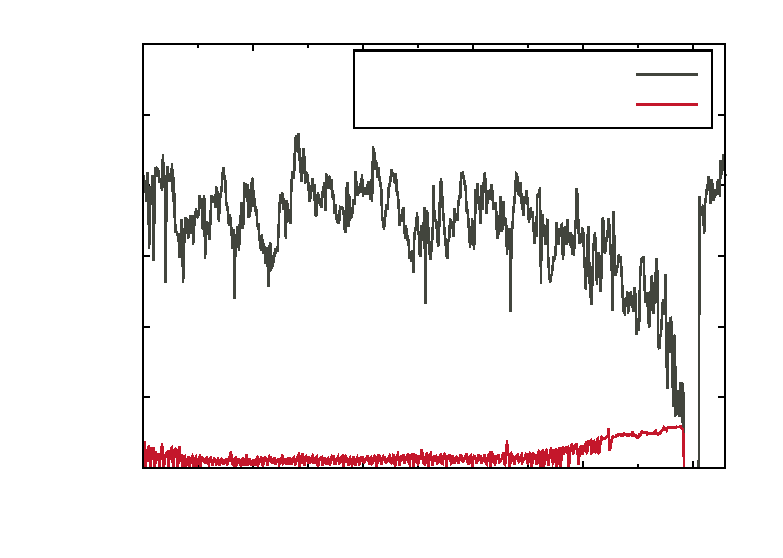
\includegraphics{graphs/restrain/clustered_restrain}}%
    \gplfronttext
  \end{picture}%
\endgroup
}
    \caption{Clustered Recovery: Requests throughput during the recovery period}
    \label{fig:restrain:clustered}
\end{figure*}


When a new application server is added, the throughput of the requests being replayed rises from 1686 to 2517 requests per second (397 seconds to recover), while the response latency to new requests is 4.61\ms. Therefore, we prove that adding more servers to perform replay allows to keep the quality of service for the customers.


%---------------------------------- replay instance ----------------------------------
%Qual o throughput maximo que uma replay instance consegue obter quando invoca directamente o application instance? Dificil de medir porque o application instance acaba por ser a limitacao quase sempre.
%The new requests are performed on new compute nodes. The \ac{HTTP} clients of each \textit{replay node} can perform \hl{XXX} request per second, using \hl{XXX} threads. (grafico a comparar com o numero de threads?)



%----------------------------------  scalability -------------------------------------
\subsubsection{Scalability}\label{sec:eval:recovery:scalability}
We measured how Shuttle leverages the horizontal scalability (adding more instances) of \ac{PaaS} to reduce the recovery period. We added \emph{c3.large} instances c3.large (7 \ac{ECU}s, 2 vCPUs, 2.8 GHz, Intel Xeon E5-2680v2, 3.75 GiB memory, 2 x 16 GiB Storage Capacity). The application server \emph{c3.xlarge} instance was downgraded to \emph{c3.large}. 

%serial
The serial replay with 2 application servers and 1 database takes 1347 seconds, while with 2 application servers an 2 database instances takes 1303 seconds (Figure \ref{fig:scalability:serial}). At larger scale, considering 2 databases, 6 application servers and 2 Shuttle storage instances, the process takes 1745\ms. Therefore, due to its implementation, the serial replay does not scale well. All instances remain with low resource usage. We expect to do much better by rewriting the implementation of the serial replay in the replay instances.

\begin{figure*}[!htb] 
    \centering
    \resizebox{0.6\linewidth}{!}{% GNUPLOT: LaTeX picture with Postscript
\begingroup
  \makeatletter
  \providecommand\color[2][]{%
    \GenericError{(gnuplot) \space\space\space\@spaces}{%
      Package color not loaded in conjunction with
      terminal option `colourtext'%
    }{See the gnuplot documentation for explanation.%
    }{Either use 'blacktext' in gnuplot or load the package
      color.sty in LaTeX.}%
    \renewcommand\color[2][]{}%
  }%
  \providecommand\includegraphics[2][]{%
    \GenericError{(gnuplot) \space\space\space\@spaces}{%
      Package graphicx or graphics not loaded%
    }{See the gnuplot documentation for explanation.%
    }{The gnuplot epslatex terminal needs graphicx.sty or graphics.sty.}%
    \renewcommand\includegraphics[2][]{}%
  }%
  \providecommand\rotatebox[2]{#2}%
  \@ifundefined{ifGPcolor}{%
    \newif\ifGPcolor
    \GPcolorfalse
  }{}%
  \@ifundefined{ifGPblacktext}{%
    \newif\ifGPblacktext
    \GPblacktexttrue
  }{}%
  % define a \g@addto@macro without @ in the name:
  \let\gplgaddtomacro\g@addto@macro
  % define empty templates for all commands taking text:
  \gdef\gplbacktext{}%
  \gdef\gplfronttext{}%
  \makeatother
  \ifGPblacktext
    % no textcolor at all
    \def\colorrgb#1{}%
    \def\colorgray#1{}%
  \else
    % gray or color?
    \ifGPcolor
      \def\colorrgb#1{\color[rgb]{#1}}%
      \def\colorgray#1{\color[gray]{#1}}%
      \expandafter\def\csname LTw\endcsname{\color{white}}%
      \expandafter\def\csname LTb\endcsname{\color{black}}%
      \expandafter\def\csname LTa\endcsname{\color{black}}%
      \expandafter\def\csname LT0\endcsname{\color[rgb]{1,0,0}}%
      \expandafter\def\csname LT1\endcsname{\color[rgb]{0,1,0}}%
      \expandafter\def\csname LT2\endcsname{\color[rgb]{0,0,1}}%
      \expandafter\def\csname LT3\endcsname{\color[rgb]{1,0,1}}%
      \expandafter\def\csname LT4\endcsname{\color[rgb]{0,1,1}}%
      \expandafter\def\csname LT5\endcsname{\color[rgb]{1,1,0}}%
      \expandafter\def\csname LT6\endcsname{\color[rgb]{0,0,0}}%
      \expandafter\def\csname LT7\endcsname{\color[rgb]{1,0.3,0}}%
      \expandafter\def\csname LT8\endcsname{\color[rgb]{0.5,0.5,0.5}}%
    \else
      % gray
      \def\colorrgb#1{\color{black}}%
      \def\colorgray#1{\color[gray]{#1}}%
      \expandafter\def\csname LTw\endcsname{\color{white}}%
      \expandafter\def\csname LTb\endcsname{\color{black}}%
      \expandafter\def\csname LTa\endcsname{\color{black}}%
      \expandafter\def\csname LT0\endcsname{\color{black}}%
      \expandafter\def\csname LT1\endcsname{\color{black}}%
      \expandafter\def\csname LT2\endcsname{\color{black}}%
      \expandafter\def\csname LT3\endcsname{\color{black}}%
      \expandafter\def\csname LT4\endcsname{\color{black}}%
      \expandafter\def\csname LT5\endcsname{\color{black}}%
      \expandafter\def\csname LT6\endcsname{\color{black}}%
      \expandafter\def\csname LT7\endcsname{\color{black}}%
      \expandafter\def\csname LT8\endcsname{\color{black}}%
    \fi
  \fi
  \setlength{\unitlength}{0.0500bp}%
  \begin{picture}(7200.00,5040.00)%
    \gplgaddtomacro\gplbacktext{%
      \csname LTb\endcsname%
      \put(1078,704){\makebox(0,0)[r]{\strut{} 0}}%
      \put(1078,1383){\makebox(0,0)[r]{\strut{} 500}}%
      \put(1078,2061){\makebox(0,0)[r]{\strut{} 1000}}%
      \put(1078,2740){\makebox(0,0)[r]{\strut{} 1500}}%
      \put(1078,3418){\makebox(0,0)[r]{\strut{} 2000}}%
      \put(1078,4097){\makebox(0,0)[r]{\strut{} 2500}}%
      \put(1078,4775){\makebox(0,0)[r]{\strut{} 3000}}%
      \put(1210,484){\makebox(0,0){\strut{}00:00}}%
      \put(1778,484){\makebox(0,0){\strut{}05:00}}%
      \put(2346,484){\makebox(0,0){\strut{}10:00}}%
      \put(2915,484){\makebox(0,0){\strut{}15:00}}%
      \put(3483,484){\makebox(0,0){\strut{}20:00}}%
      \put(4051,484){\makebox(0,0){\strut{}25:00}}%
      \put(4619,484){\makebox(0,0){\strut{}30:00}}%
      \put(5187,484){\makebox(0,0){\strut{}35:00}}%
      \put(5756,484){\makebox(0,0){\strut{}40:00}}%
      \put(6324,484){\makebox(0,0){\strut{}45:00}}%
      \put(176,2739){\rotatebox{-270}{\makebox(0,0){\strut{}Requests per second}}}%
      \put(4006,154){\makebox(0,0){\strut{}Time (minutes:seconds)}}%
      \put(4714,3418){\makebox(0,0)[l]{\strut{}Restrain}}%
    }%
    \gplgaddtomacro\gplfronttext{%
      \csname LTb\endcsname%
      \put(5816,4481){\makebox(0,0)[r]{\strut{}graphs/restrain/graphs/restrain/graphs/restrain/graphs/restrain/graphs/restrain/graphs/restrain/serial replay}}%
      \csname LTb\endcsname%
      \put(5816,4195){\makebox(0,0)[r]{\strut{}concurrent client}}%
    }%
    \gplbacktext
    \put(0,0){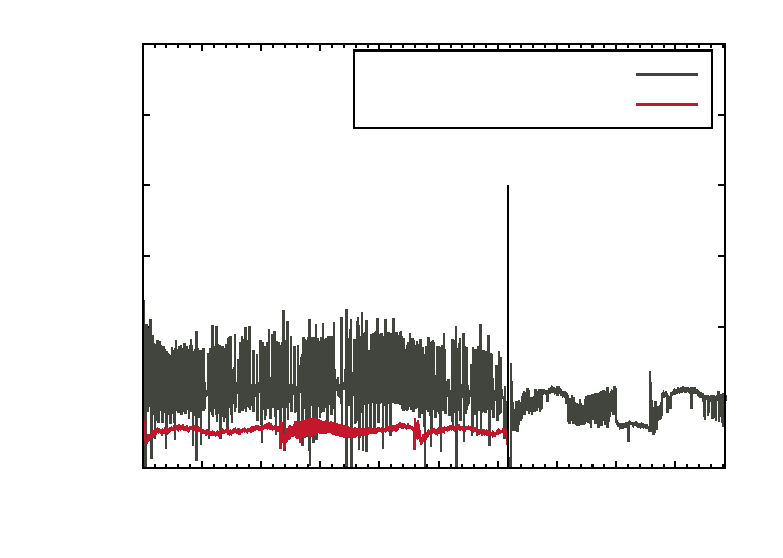
\includegraphics{graphs/restrain/graphs/restrain/graphs/restrain/graphs/restrain/graphs/restrain/graphs/restrain/graphs/restrain/serial}}%
    \gplfronttext
  \end{picture}%
\endgroup
}
    \caption{Shuttle Scalability Serial}
    \label{fig:scalability:serial}
\end{figure*}


%parallel
The Figure \ref{fig:scalability} (detailed values in Appendix \ref{appendix:results}) shows the recovery time using clustered replay. The figure demonstrates that Shuttle is scalable, in the sense that adding more servers allow reducing the time of recovery. Three application servers allowed recovery in half the time of one (750 versus 417 seconds). If the application runs on 5 or more application servers, then the single Shuttle Storage (Cassandra) instance becomes the bottleneck because Shuttle database client interceptor fetches the keys accessed by every request. We added another \emph{c3.xlarge} instance to the Cassandra cluster. 
\hl{reler esta seccao toda}
The latency of the requests during their first execution remains approximately constant when 3 servers are added (Figure \ref{fig:recovery_scalability:latency}). This means that a single \emph{TryOut} instance performing 2000 requests per second is not capable of overstraining the resources of the application servers.

\begin{figure*}[!htb]
  \centering
  \subfloat[][Recovery time (Clustered replay)]{
      \resizebox{0.5\linewidth}{!}{% GNUPLOT: LaTeX picture with Postscript
\begingroup
  \makeatletter
  \providecommand\color[2][]{%
    \GenericError{(gnuplot) \space\space\space\@spaces}{%
      Package color not loaded in conjunction with
      terminal option `colourtext'%
    }{See the gnuplot documentation for explanation.%
    }{Either use 'blacktext' in gnuplot or load the package
      color.sty in LaTeX.}%
    \renewcommand\color[2][]{}%
  }%
  \providecommand\includegraphics[2][]{%
    \GenericError{(gnuplot) \space\space\space\@spaces}{%
      Package graphicx or graphics not loaded%
    }{See the gnuplot documentation for explanation.%
    }{The gnuplot epslatex terminal needs graphicx.sty or graphics.sty.}%
    \renewcommand\includegraphics[2][]{}%
  }%
  \providecommand\rotatebox[2]{#2}%
  \@ifundefined{ifGPcolor}{%
    \newif\ifGPcolor
    \GPcolorfalse
  }{}%
  \@ifundefined{ifGPblacktext}{%
    \newif\ifGPblacktext
    \GPblacktexttrue
  }{}%
  % define a \g@addto@macro without @ in the name:
  \let\gplgaddtomacro\g@addto@macro
  % define empty templates for all commands taking text:
  \gdef\gplbacktext{}%
  \gdef\gplfronttext{}%
  \makeatother
  \ifGPblacktext
    % no textcolor at all
    \def\colorrgb#1{}%
    \def\colorgray#1{}%
  \else
    % gray or color?
    \ifGPcolor
      \def\colorrgb#1{\color[rgb]{#1}}%
      \def\colorgray#1{\color[gray]{#1}}%
      \expandafter\def\csname LTw\endcsname{\color{white}}%
      \expandafter\def\csname LTb\endcsname{\color{black}}%
      \expandafter\def\csname LTa\endcsname{\color{black}}%
      \expandafter\def\csname LT0\endcsname{\color[rgb]{1,0,0}}%
      \expandafter\def\csname LT1\endcsname{\color[rgb]{0,1,0}}%
      \expandafter\def\csname LT2\endcsname{\color[rgb]{0,0,1}}%
      \expandafter\def\csname LT3\endcsname{\color[rgb]{1,0,1}}%
      \expandafter\def\csname LT4\endcsname{\color[rgb]{0,1,1}}%
      \expandafter\def\csname LT5\endcsname{\color[rgb]{1,1,0}}%
      \expandafter\def\csname LT6\endcsname{\color[rgb]{0,0,0}}%
      \expandafter\def\csname LT7\endcsname{\color[rgb]{1,0.3,0}}%
      \expandafter\def\csname LT8\endcsname{\color[rgb]{0.5,0.5,0.5}}%
    \else
      % gray
      \def\colorrgb#1{\color{black}}%
      \def\colorgray#1{\color[gray]{#1}}%
      \expandafter\def\csname LTw\endcsname{\color{white}}%
      \expandafter\def\csname LTb\endcsname{\color{black}}%
      \expandafter\def\csname LTa\endcsname{\color{black}}%
      \expandafter\def\csname LT0\endcsname{\color{black}}%
      \expandafter\def\csname LT1\endcsname{\color{black}}%
      \expandafter\def\csname LT2\endcsname{\color{black}}%
      \expandafter\def\csname LT3\endcsname{\color{black}}%
      \expandafter\def\csname LT4\endcsname{\color{black}}%
      \expandafter\def\csname LT5\endcsname{\color{black}}%
      \expandafter\def\csname LT6\endcsname{\color{black}}%
      \expandafter\def\csname LT7\endcsname{\color{black}}%
      \expandafter\def\csname LT8\endcsname{\color{black}}%
    \fi
  \fi
  \setlength{\unitlength}{0.0500bp}%
  \begin{picture}(7200.00,5040.00)%
    \gplgaddtomacro\gplbacktext{%
      \csname LTb\endcsname%
      \put(946,704){\makebox(0,0)[r]{\strut{} 0}}%
      \put(946,1156){\makebox(0,0)[r]{\strut{} 100}}%
      \put(946,1609){\makebox(0,0)[r]{\strut{} 200}}%
      \put(946,2061){\makebox(0,0)[r]{\strut{} 300}}%
      \put(946,2513){\makebox(0,0)[r]{\strut{} 400}}%
      \put(946,2966){\makebox(0,0)[r]{\strut{} 500}}%
      \put(946,3418){\makebox(0,0)[r]{\strut{} 600}}%
      \put(946,3870){\makebox(0,0)[r]{\strut{} 700}}%
      \put(946,4323){\makebox(0,0)[r]{\strut{} 800}}%
      \put(946,4775){\makebox(0,0)[r]{\strut{} 900}}%
      \put(1078,484){\makebox(0,0){\strut{} 0}}%
      \put(1896,484){\makebox(0,0){\strut{} 1}}%
      \put(2714,484){\makebox(0,0){\strut{} 2}}%
      \put(3532,484){\makebox(0,0){\strut{} 3}}%
      \put(4349,484){\makebox(0,0){\strut{} 4}}%
      \put(5167,484){\makebox(0,0){\strut{} 5}}%
      \put(5985,484){\makebox(0,0){\strut{} 6}}%
      \put(6803,484){\makebox(0,0){\strut{} 7}}%
      \put(176,2739){\rotatebox{-270}{\makebox(0,0){\strut{}Time to recovery (seconds)}}}%
      \put(3940,154){\makebox(0,0){\strut{}Number of application servers}}%
    }%
    \gplgaddtomacro\gplfronttext{%
      \csname LTb\endcsname%
      \put(5816,4481){\makebox(0,0)[r]{\strut{}1 replay and 1 DB instance}}%
    }%
    \gplbacktext
    \put(0,0){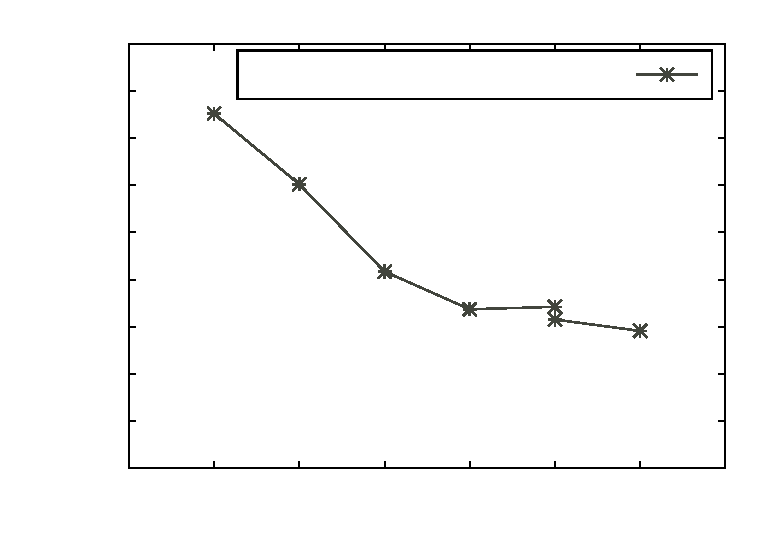
\includegraphics{graphs/scalability/recovery_time}}%
    \gplfronttext
  \end{picture}%
\endgroup
\label{fig:recovery_scalability}}
  } 
  \subfloat[][Response latency on first execution]{
      \resizebox{0.5\linewidth}{!}{% GNUPLOT: LaTeX picture with Postscript
\begingroup
  \makeatletter
  \providecommand\color[2][]{%
    \GenericError{(gnuplot) \space\space\space\@spaces}{%
      Package color not loaded in conjunction with
      terminal option `colourtext'%
    }{See the gnuplot documentation for explanation.%
    }{Either use 'blacktext' in gnuplot or load the package
      color.sty in LaTeX.}%
    \renewcommand\color[2][]{}%
  }%
  \providecommand\includegraphics[2][]{%
    \GenericError{(gnuplot) \space\space\space\@spaces}{%
      Package graphicx or graphics not loaded%
    }{See the gnuplot documentation for explanation.%
    }{The gnuplot epslatex terminal needs graphicx.sty or graphics.sty.}%
    \renewcommand\includegraphics[2][]{}%
  }%
  \providecommand\rotatebox[2]{#2}%
  \@ifundefined{ifGPcolor}{%
    \newif\ifGPcolor
    \GPcolorfalse
  }{}%
  \@ifundefined{ifGPblacktext}{%
    \newif\ifGPblacktext
    \GPblacktexttrue
  }{}%
  % define a \g@addto@macro without @ in the name:
  \let\gplgaddtomacro\g@addto@macro
  % define empty templates for all commands taking text:
  \gdef\gplbacktext{}%
  \gdef\gplfronttext{}%
  \makeatother
  \ifGPblacktext
    % no textcolor at all
    \def\colorrgb#1{}%
    \def\colorgray#1{}%
  \else
    % gray or color?
    \ifGPcolor
      \def\colorrgb#1{\color[rgb]{#1}}%
      \def\colorgray#1{\color[gray]{#1}}%
      \expandafter\def\csname LTw\endcsname{\color{white}}%
      \expandafter\def\csname LTb\endcsname{\color{black}}%
      \expandafter\def\csname LTa\endcsname{\color{black}}%
      \expandafter\def\csname LT0\endcsname{\color[rgb]{1,0,0}}%
      \expandafter\def\csname LT1\endcsname{\color[rgb]{0,1,0}}%
      \expandafter\def\csname LT2\endcsname{\color[rgb]{0,0,1}}%
      \expandafter\def\csname LT3\endcsname{\color[rgb]{1,0,1}}%
      \expandafter\def\csname LT4\endcsname{\color[rgb]{0,1,1}}%
      \expandafter\def\csname LT5\endcsname{\color[rgb]{1,1,0}}%
      \expandafter\def\csname LT6\endcsname{\color[rgb]{0,0,0}}%
      \expandafter\def\csname LT7\endcsname{\color[rgb]{1,0.3,0}}%
      \expandafter\def\csname LT8\endcsname{\color[rgb]{0.5,0.5,0.5}}%
    \else
      % gray
      \def\colorrgb#1{\color{black}}%
      \def\colorgray#1{\color[gray]{#1}}%
      \expandafter\def\csname LTw\endcsname{\color{white}}%
      \expandafter\def\csname LTb\endcsname{\color{black}}%
      \expandafter\def\csname LTa\endcsname{\color{black}}%
      \expandafter\def\csname LT0\endcsname{\color{black}}%
      \expandafter\def\csname LT1\endcsname{\color{black}}%
      \expandafter\def\csname LT2\endcsname{\color{black}}%
      \expandafter\def\csname LT3\endcsname{\color{black}}%
      \expandafter\def\csname LT4\endcsname{\color{black}}%
      \expandafter\def\csname LT5\endcsname{\color{black}}%
      \expandafter\def\csname LT6\endcsname{\color{black}}%
      \expandafter\def\csname LT7\endcsname{\color{black}}%
      \expandafter\def\csname LT8\endcsname{\color{black}}%
    \fi
  \fi
  \setlength{\unitlength}{0.0500bp}%
  \begin{picture}(7200.00,5040.00)%
    \gplgaddtomacro\gplbacktext{%
      \csname LTb\endcsname%
      \put(814,704){\makebox(0,0)[r]{\strut{} 0}}%
      \put(814,1383){\makebox(0,0)[r]{\strut{} 5}}%
      \put(814,2061){\makebox(0,0)[r]{\strut{} 10}}%
      \put(814,2740){\makebox(0,0)[r]{\strut{} 15}}%
      \put(814,3418){\makebox(0,0)[r]{\strut{} 20}}%
      \put(814,4097){\makebox(0,0)[r]{\strut{} 25}}%
      \put(814,4775){\makebox(0,0)[r]{\strut{} 30}}%
      \put(946,484){\makebox(0,0){\strut{} 0}}%
      \put(1783,484){\makebox(0,0){\strut{} 1}}%
      \put(2619,484){\makebox(0,0){\strut{} 2}}%
      \put(3456,484){\makebox(0,0){\strut{} 3}}%
      \put(4293,484){\makebox(0,0){\strut{} 4}}%
      \put(5130,484){\makebox(0,0){\strut{} 5}}%
      \put(5966,484){\makebox(0,0){\strut{} 6}}%
      \put(6803,484){\makebox(0,0){\strut{} 7}}%
      \put(176,2739){\rotatebox{-270}{\makebox(0,0){\strut{}Request latency (ms)}}}%
      \put(3874,154){\makebox(0,0){\strut{}Number of servers}}%
    }%
    \gplgaddtomacro\gplfronttext{%
      \csname LTb\endcsname%
      \put(5816,4481){\makebox(0,0)[r]{\strut{}1 replay and 1 DB instance}}%
    }%
    \gplbacktext
    \put(0,0){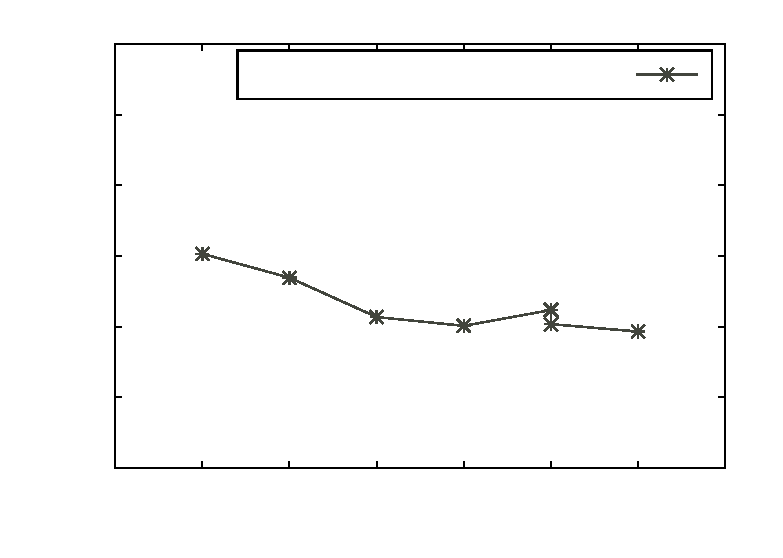
\includegraphics{graphs/scalability/latencia}}%
    \gplfronttext
  \end{picture}%
\endgroup
\label{fig:recovery_scalability:latency}}
  } 
  \caption{Shuttle Scalability}
  \label{fig:scalability}
\end{figure*}

When using less than 6 application servers, adding more database instances or clients does not improve the performance. When supporting 3 application servers, the \ac{CPU} usage of Voldemort database remains at 10\% on average. The \ac{CPU} usage of the instances that contain Shuttle's modules remains low (Figure \ref{fig:scalability:cpu:shuttle}). The bottleneck is the \ac{CPU} usage on the application servers (Figure \ref{fig:scalability:cpu:app}).

\begin{figure*}[!htb]
  \centering
  \subfloat[][CPU usage of Shuttle's instances ]{
      \resizebox{0.5\linewidth}{!}{% GNUPLOT: LaTeX picture with Postscript
\begingroup
  \makeatletter
  \providecommand\color[2][]{%
    \GenericError{(gnuplot) \space\space\space\@spaces}{%
      Package color not loaded in conjunction with
      terminal option `colourtext'%
    }{See the gnuplot documentation for explanation.%
    }{Either use 'blacktext' in gnuplot or load the package
      color.sty in LaTeX.}%
    \renewcommand\color[2][]{}%
  }%
  \providecommand\includegraphics[2][]{%
    \GenericError{(gnuplot) \space\space\space\@spaces}{%
      Package graphicx or graphics not loaded%
    }{See the gnuplot documentation for explanation.%
    }{The gnuplot epslatex terminal needs graphicx.sty or graphics.sty.}%
    \renewcommand\includegraphics[2][]{}%
  }%
  \providecommand\rotatebox[2]{#2}%
  \@ifundefined{ifGPcolor}{%
    \newif\ifGPcolor
    \GPcolorfalse
  }{}%
  \@ifundefined{ifGPblacktext}{%
    \newif\ifGPblacktext
    \GPblacktexttrue
  }{}%
  % define a \g@addto@macro without @ in the name:
  \let\gplgaddtomacro\g@addto@macro
  % define empty templates for all commands taking text:
  \gdef\gplbacktext{}%
  \gdef\gplfronttext{}%
  \makeatother
  \ifGPblacktext
    % no textcolor at all
    \def\colorrgb#1{}%
    \def\colorgray#1{}%
  \else
    % gray or color?
    \ifGPcolor
      \def\colorrgb#1{\color[rgb]{#1}}%
      \def\colorgray#1{\color[gray]{#1}}%
      \expandafter\def\csname LTw\endcsname{\color{white}}%
      \expandafter\def\csname LTb\endcsname{\color{black}}%
      \expandafter\def\csname LTa\endcsname{\color{black}}%
      \expandafter\def\csname LT0\endcsname{\color[rgb]{1,0,0}}%
      \expandafter\def\csname LT1\endcsname{\color[rgb]{0,1,0}}%
      \expandafter\def\csname LT2\endcsname{\color[rgb]{0,0,1}}%
      \expandafter\def\csname LT3\endcsname{\color[rgb]{1,0,1}}%
      \expandafter\def\csname LT4\endcsname{\color[rgb]{0,1,1}}%
      \expandafter\def\csname LT5\endcsname{\color[rgb]{1,1,0}}%
      \expandafter\def\csname LT6\endcsname{\color[rgb]{0,0,0}}%
      \expandafter\def\csname LT7\endcsname{\color[rgb]{1,0.3,0}}%
      \expandafter\def\csname LT8\endcsname{\color[rgb]{0.5,0.5,0.5}}%
    \else
      % gray
      \def\colorrgb#1{\color{black}}%
      \def\colorgray#1{\color[gray]{#1}}%
      \expandafter\def\csname LTw\endcsname{\color{white}}%
      \expandafter\def\csname LTb\endcsname{\color{black}}%
      \expandafter\def\csname LTa\endcsname{\color{black}}%
      \expandafter\def\csname LT0\endcsname{\color{black}}%
      \expandafter\def\csname LT1\endcsname{\color{black}}%
      \expandafter\def\csname LT2\endcsname{\color{black}}%
      \expandafter\def\csname LT3\endcsname{\color{black}}%
      \expandafter\def\csname LT4\endcsname{\color{black}}%
      \expandafter\def\csname LT5\endcsname{\color{black}}%
      \expandafter\def\csname LT6\endcsname{\color{black}}%
      \expandafter\def\csname LT7\endcsname{\color{black}}%
      \expandafter\def\csname LT8\endcsname{\color{black}}%
    \fi
  \fi
  \setlength{\unitlength}{0.0500bp}%
  \begin{picture}(7200.00,5040.00)%
    \gplgaddtomacro\gplbacktext{%
      \csname LTb\endcsname%
      \put(946,704){\makebox(0,0)[r]{\strut{} 0}}%
      \put(946,1111){\makebox(0,0)[r]{\strut{} 10}}%
      \put(946,1518){\makebox(0,0)[r]{\strut{} 20}}%
      \put(946,1925){\makebox(0,0)[r]{\strut{} 30}}%
      \put(946,2332){\makebox(0,0)[r]{\strut{} 40}}%
      \put(946,2740){\makebox(0,0)[r]{\strut{} 50}}%
      \put(946,3147){\makebox(0,0)[r]{\strut{} 60}}%
      \put(946,3554){\makebox(0,0)[r]{\strut{} 70}}%
      \put(946,3961){\makebox(0,0)[r]{\strut{} 80}}%
      \put(946,4368){\makebox(0,0)[r]{\strut{} 90}}%
      \put(946,4775){\makebox(0,0)[r]{\strut{} 100}}%
      \put(1078,484){\makebox(0,0){\strut{}00:00}}%
      \put(2223,484){\makebox(0,0){\strut{}02:00}}%
      \put(3368,484){\makebox(0,0){\strut{}04:00}}%
      \put(4513,484){\makebox(0,0){\strut{}06:00}}%
      \put(5658,484){\makebox(0,0){\strut{}08:00}}%
      \put(6803,484){\makebox(0,0){\strut{}10:00}}%
      \put(176,2739){\rotatebox{-270}{\makebox(0,0){\strut{}Maximum CPU Utilization (\%)}}}%
      \put(3940,154){\makebox(0,0){\strut{}Time (Hour:Minute)}}%
    }%
    \gplgaddtomacro\gplfronttext{%
      \csname LTb\endcsname%
      \put(5816,4481){\makebox(0,0)[r]{\strut{}HA Proxy + Proxy}}%
      \csname LTb\endcsname%
      \put(5816,4195){\makebox(0,0)[r]{\strut{}Replay Instance I + TryOut}}%
      \csname LTb\endcsname%
      \put(5816,3909){\makebox(0,0)[r]{\strut{}Manager + Cassandra I + Replay II}}%
    }%
    \gplbacktext
    \put(0,0){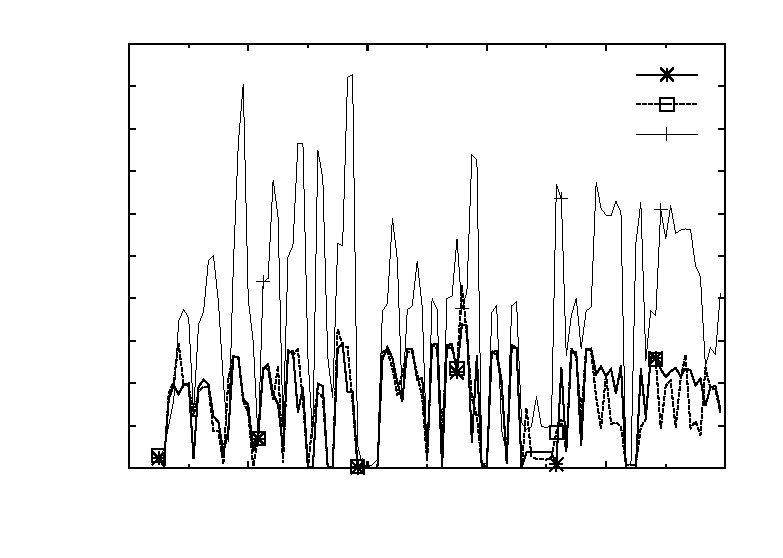
\includegraphics{graphs/usage/cpu_shuttle}}%
    \gplfronttext
  \end{picture}%
\endgroup
\label{fig:scalability:cpu:shuttle}}
  } 
  \subfloat[][CPU usage of Application instances ]{
      \resizebox{0.5\linewidth}{!}{% GNUPLOT: LaTeX picture with Postscript
\begingroup
  \makeatletter
  \providecommand\color[2][]{%
    \GenericError{(gnuplot) \space\space\space\@spaces}{%
      Package color not loaded in conjunction with
      terminal option `colourtext'%
    }{See the gnuplot documentation for explanation.%
    }{Either use 'blacktext' in gnuplot or load the package
      color.sty in LaTeX.}%
    \renewcommand\color[2][]{}%
  }%
  \providecommand\includegraphics[2][]{%
    \GenericError{(gnuplot) \space\space\space\@spaces}{%
      Package graphicx or graphics not loaded%
    }{See the gnuplot documentation for explanation.%
    }{The gnuplot epslatex terminal needs graphicx.sty or graphics.sty.}%
    \renewcommand\includegraphics[2][]{}%
  }%
  \providecommand\rotatebox[2]{#2}%
  \@ifundefined{ifGPcolor}{%
    \newif\ifGPcolor
    \GPcolorfalse
  }{}%
  \@ifundefined{ifGPblacktext}{%
    \newif\ifGPblacktext
    \GPblacktexttrue
  }{}%
  % define a \g@addto@macro without @ in the name:
  \let\gplgaddtomacro\g@addto@macro
  % define empty templates for all commands taking text:
  \gdef\gplbacktext{}%
  \gdef\gplfronttext{}%
  \makeatother
  \ifGPblacktext
    % no textcolor at all
    \def\colorrgb#1{}%
    \def\colorgray#1{}%
  \else
    % gray or color?
    \ifGPcolor
      \def\colorrgb#1{\color[rgb]{#1}}%
      \def\colorgray#1{\color[gray]{#1}}%
      \expandafter\def\csname LTw\endcsname{\color{white}}%
      \expandafter\def\csname LTb\endcsname{\color{black}}%
      \expandafter\def\csname LTa\endcsname{\color{black}}%
      \expandafter\def\csname LT0\endcsname{\color[rgb]{1,0,0}}%
      \expandafter\def\csname LT1\endcsname{\color[rgb]{0,1,0}}%
      \expandafter\def\csname LT2\endcsname{\color[rgb]{0,0,1}}%
      \expandafter\def\csname LT3\endcsname{\color[rgb]{1,0,1}}%
      \expandafter\def\csname LT4\endcsname{\color[rgb]{0,1,1}}%
      \expandafter\def\csname LT5\endcsname{\color[rgb]{1,1,0}}%
      \expandafter\def\csname LT6\endcsname{\color[rgb]{0,0,0}}%
      \expandafter\def\csname LT7\endcsname{\color[rgb]{1,0.3,0}}%
      \expandafter\def\csname LT8\endcsname{\color[rgb]{0.5,0.5,0.5}}%
    \else
      % gray
      \def\colorrgb#1{\color{black}}%
      \def\colorgray#1{\color[gray]{#1}}%
      \expandafter\def\csname LTw\endcsname{\color{white}}%
      \expandafter\def\csname LTb\endcsname{\color{black}}%
      \expandafter\def\csname LTa\endcsname{\color{black}}%
      \expandafter\def\csname LT0\endcsname{\color{black}}%
      \expandafter\def\csname LT1\endcsname{\color{black}}%
      \expandafter\def\csname LT2\endcsname{\color{black}}%
      \expandafter\def\csname LT3\endcsname{\color{black}}%
      \expandafter\def\csname LT4\endcsname{\color{black}}%
      \expandafter\def\csname LT5\endcsname{\color{black}}%
      \expandafter\def\csname LT6\endcsname{\color{black}}%
      \expandafter\def\csname LT7\endcsname{\color{black}}%
      \expandafter\def\csname LT8\endcsname{\color{black}}%
    \fi
  \fi
  \setlength{\unitlength}{0.0500bp}%
  \begin{picture}(7200.00,5040.00)%
    \gplgaddtomacro\gplbacktext{%
      \csname LTb\endcsname%
      \put(946,704){\makebox(0,0)[r]{\strut{} 0}}%
      \put(946,1518){\makebox(0,0)[r]{\strut{} 20}}%
      \put(946,2332){\makebox(0,0)[r]{\strut{} 40}}%
      \put(946,3147){\makebox(0,0)[r]{\strut{} 60}}%
      \put(946,3961){\makebox(0,0)[r]{\strut{} 80}}%
      \put(946,4775){\makebox(0,0)[r]{\strut{} 100}}%
      \put(1078,484){\makebox(0,0){\strut{}00:00}}%
      \put(1894,484){\makebox(0,0){\strut{}02:00}}%
      \put(2709,484){\makebox(0,0){\strut{}04:00}}%
      \put(3525,484){\makebox(0,0){\strut{}06:00}}%
      \put(4340,484){\makebox(0,0){\strut{}08:00}}%
      \put(5156,484){\makebox(0,0){\strut{}10:00}}%
      \put(176,2739){\rotatebox{-270}{\makebox(0,0){\strut{}Maximum CPU Utilization (\%)}}}%
      \put(3117,154){\makebox(0,0){\strut{}Time (Hour:Minute)}}%
    }%
    \gplgaddtomacro\gplfronttext{%
      \csname LTb\endcsname%
      \put(6212,4544){\makebox(0,0)[r]{\strut{}Server II }}%
      \csname LTb\endcsname%
      \put(6212,4258){\makebox(0,0)[r]{\strut{}Server III }}%
      \csname LTb\endcsname%
      \put(6212,3972){\makebox(0,0)[r]{\strut{}Server IV }}%
      \csname LTb\endcsname%
      \put(6212,3686){\makebox(0,0)[r]{\strut{}Server V }}%
      \csname LTb\endcsname%
      \put(6212,3400){\makebox(0,0)[r]{\strut{}Server VI }}%
    }%
    \gplbacktext
    \put(0,0){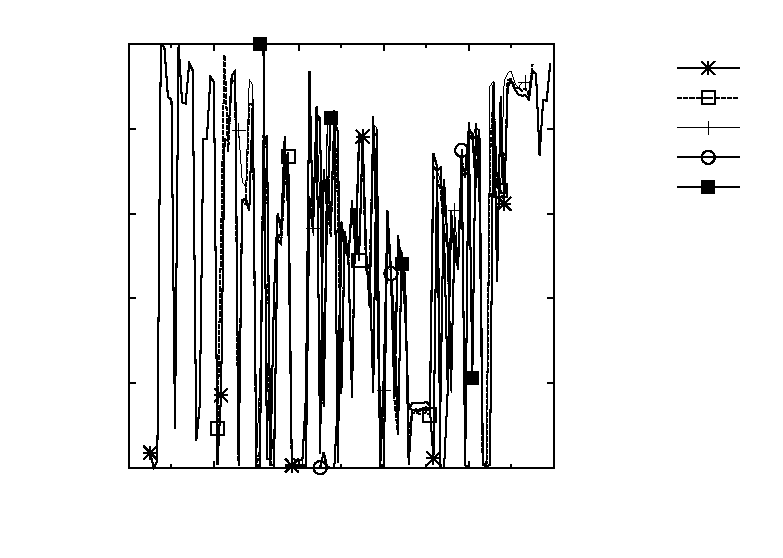
\includegraphics{graphs/usage/cpu_app}}%
    \gplfronttext
  \end{picture}%
\endgroup
\label{fig:scalability:cpu:app}}
  } 
  \caption{CPU Usage during several execution and replay phases}
  \label{fig:scalability:cpu}
\end{figure*}

%In \emph{Ask}, the voting requests represent 4\% of the total number of requests. These requests only increment a variable. Incrementar uma variavel ate 1000 implica 1000 requests enquanto que saber o seu valor e fazer set a 1000 implicaria apenas 1 request.

We conclude the application servers to be the main performance harm. The performance of the application servers can be improved. If application developers for \ac{PaaS} optimize their applications to execute more requests per unit of time, then the recovery period is reduced. %Shuttle's scalability depends on its algorithms and implementation
Most of \ac{PaaS} controller watch the load of the instances. One area of future development is to dynamically adapt the throughput of the replay instances to the load of the application and database instances.



%If a new database instance is added, then the delay is \hl{xxxx} and the throughput of the replaying requests is \hl{xxxx}.
%The recovery period varies with the dependencies between requests. Shuttle reduces the recovery period by replaying independent clusters in parallel. 
% \begin{figure*}[!htb]
%     \resizebox{0.5\linewidth}{!}{% GNUPLOT: LaTeX picture with Postscript
\begingroup
  \makeatletter
  \providecommand\color[2][]{%
    \GenericError{(gnuplot) \space\space\space\@spaces}{%
      Package color not loaded in conjunction with
      terminal option `colourtext'%
    }{See the gnuplot documentation for explanation.%
    }{Either use 'blacktext' in gnuplot or load the package
      color.sty in LaTeX.}%
    \renewcommand\color[2][]{}%
  }%
  \providecommand\includegraphics[2][]{%
    \GenericError{(gnuplot) \space\space\space\@spaces}{%
      Package graphicx or graphics not loaded%
    }{See the gnuplot documentation for explanation.%
    }{The gnuplot epslatex terminal needs graphicx.sty or graphics.sty.}%
    \renewcommand\includegraphics[2][]{}%
  }%
  \providecommand\rotatebox[2]{#2}%
  \@ifundefined{ifGPcolor}{%
    \newif\ifGPcolor
    \GPcolorfalse
  }{}%
  \@ifundefined{ifGPblacktext}{%
    \newif\ifGPblacktext
    \GPblacktexttrue
  }{}%
  % define a \g@addto@macro without @ in the name:
  \let\gplgaddtomacro\g@addto@macro
  % define empty templates for all commands taking text:
  \gdef\gplbacktext{}%
  \gdef\gplfronttext{}%
  \makeatother
  \ifGPblacktext
    % no textcolor at all
    \def\colorrgb#1{}%
    \def\colorgray#1{}%
  \else
    % gray or color?
    \ifGPcolor
      \def\colorrgb#1{\color[rgb]{#1}}%
      \def\colorgray#1{\color[gray]{#1}}%
      \expandafter\def\csname LTw\endcsname{\color{white}}%
      \expandafter\def\csname LTb\endcsname{\color{black}}%
      \expandafter\def\csname LTa\endcsname{\color{black}}%
      \expandafter\def\csname LT0\endcsname{\color[rgb]{1,0,0}}%
      \expandafter\def\csname LT1\endcsname{\color[rgb]{0,1,0}}%
      \expandafter\def\csname LT2\endcsname{\color[rgb]{0,0,1}}%
      \expandafter\def\csname LT3\endcsname{\color[rgb]{1,0,1}}%
      \expandafter\def\csname LT4\endcsname{\color[rgb]{0,1,1}}%
      \expandafter\def\csname LT5\endcsname{\color[rgb]{1,1,0}}%
      \expandafter\def\csname LT6\endcsname{\color[rgb]{0,0,0}}%
      \expandafter\def\csname LT7\endcsname{\color[rgb]{1,0.3,0}}%
      \expandafter\def\csname LT8\endcsname{\color[rgb]{0.5,0.5,0.5}}%
    \else
      % gray
      \def\colorrgb#1{\color{black}}%
      \def\colorgray#1{\color[gray]{#1}}%
      \expandafter\def\csname LTw\endcsname{\color{white}}%
      \expandafter\def\csname LTb\endcsname{\color{black}}%
      \expandafter\def\csname LTa\endcsname{\color{black}}%
      \expandafter\def\csname LT0\endcsname{\color{black}}%
      \expandafter\def\csname LT1\endcsname{\color{black}}%
      \expandafter\def\csname LT2\endcsname{\color{black}}%
      \expandafter\def\csname LT3\endcsname{\color{black}}%
      \expandafter\def\csname LT4\endcsname{\color{black}}%
      \expandafter\def\csname LT5\endcsname{\color{black}}%
      \expandafter\def\csname LT6\endcsname{\color{black}}%
      \expandafter\def\csname LT7\endcsname{\color{black}}%
      \expandafter\def\csname LT8\endcsname{\color{black}}%
    \fi
  \fi
  \setlength{\unitlength}{0.0500bp}%
  \begin{picture}(7200.00,5040.00)%
    \gplgaddtomacro\gplbacktext{%
      \csname LTb\endcsname%
      \put(1078,704){\makebox(0,0)[r]{\strut{} 20}}%
      \put(1078,1518){\makebox(0,0)[r]{\strut{} 20.2}}%
      \put(1078,2332){\makebox(0,0)[r]{\strut{} 20.4}}%
      \put(1078,3147){\makebox(0,0)[r]{\strut{} 20.6}}%
      \put(1078,3961){\makebox(0,0)[r]{\strut{} 20.8}}%
      \put(1078,4775){\makebox(0,0)[r]{\strut{} 21}}%
      \put(1210,484){\makebox(0,0){\strut{} 0}}%
      \put(2142,484){\makebox(0,0){\strut{} 2}}%
      \put(3074,484){\makebox(0,0){\strut{} 4}}%
      \put(4007,484){\makebox(0,0){\strut{} 6}}%
      \put(4939,484){\makebox(0,0){\strut{} 8}}%
      \put(5871,484){\makebox(0,0){\strut{} 10}}%
      \put(6803,484){\makebox(0,0){\strut{} 12}}%
      \put(176,2739){\rotatebox{-270}{\makebox(0,0){\strut{}Recovery time (ms)}}}%
      \put(4006,154){\makebox(0,0){\strut{}Number of requests}}%
    }%
    \gplgaddtomacro\gplfronttext{%
      \csname LTb\endcsname%
      \put(5816,4602){\makebox(0,0)[r]{\strut{}1 Cluster}}%
      \csname LTb\endcsname%
      \put(5816,4382){\makebox(0,0)[r]{\strut{}2 Clusters}}%
      \csname LTb\endcsname%
      \put(5816,4162){\makebox(0,0)[r]{\strut{}3 Cluster}}%
      \csname LTb\endcsname%
      \put(5816,3942){\makebox(0,0)[r]{\strut{}4 Clusters}}%
      \csname LTb\endcsname%
      \put(5816,3722){\makebox(0,0)[r]{\strut{}5 Clusters}}%
    }%
    \gplbacktext
    \put(0,0){\includegraphics{graphs/clusters/grafico}}%
    \gplfronttext
  \end{picture}%
\endgroup
}
%     \caption{\textbf{Clustering influence on recovery time: throughput vs clustering: 1 cluster, 10 clusters, 100 clusters, 1000 clusters, 10000 clusters}}
%     \label{fig:clustering_influence}
% \end{figure*}


%%%%%%%%%%%%%%%%%%%%%%%%%%%%%%%%%%%%%%%%%%%%%%%%%%%%%%%%%%%%%%%%%%%%%%%%%%%%%%%%%%%%%%%%%%%%%%%%%%%%%%%%%%%%%%%%
\subsection{Space Overhead}\label{sec:eval:storage}
The storage overhead is relevant because it is a payed cloud resource and Shuttle stores every user request. The space overhead is defined by the variables in Table \ref{tab:storage_variables}.

\begin{table}[ht]
\centering
\begin{tabular}{l|ll}
\textbf{Module}          & \textbf{Contains}      & \textbf{Depends on}    \\ \hline
\textbf{Shuttle Storage} &                        &                          \\
                         & Request                & request content          \\
                         & Response (optional)    & response content         \\
                         & Accessed keys          & key size and number of database operations per request\\
                         & Start and end instants & constant overhead           \\ \hline
\textbf{Database instance} &                      &                          \\
                          & Version list          & number of snapshots per data item \\
                          & Operation list        & number of operations per data item \\ \hline
\textbf{Dependency graph} &                       &                                   \\
                        & Dependencies            & number of dependencies per request\\
\end{tabular}
\caption{Variables on Shuttle's storage}
\label{tab:storage_variables}
\end{table}

Requests to static contents, e.g., images, are ignored. For instance, a question page of StackOverflow \cite{stackoverflow} implies 30 static content requests. Shuttle is not implemented for web-services with large requests, such has file hosting services, because the data would be duplicated in the requests and storage. Shuttle architecture would remain similar on those services but would require an algorithm to reduce the storage overhead by detecting duplicated data.\\

%define request size
Most of applications' requests, including headers, vary in size from 200 bytes to over 2KB, depending on the number of application cookies \cite{spdy}. As applications use more cookies and user agents expand features, typical header sizes of 700-800 bytes are common \cite{spdy}. Shuttle adds the \ac{SRD}, which has 35 bytes, to every request. Requests of \emph{Ask} based on the StackExchange Network have an average size of 216 bytes (std. def of 124 bytes, 95th percentile of 274 bytes,  99th of 494 bytes in a sample of 200 thousand requests, in which 95\% are read requests).

%shuttle storage
Requests and keys are stored in the \emph{Shuttle storage} (Cassandra) while the dependency graph and database operations are kept in  manager and database instances. Values at Table \ref{tab:storage_overhead} represent the size of each component in memory \footnote{https://code.google.com/p/memory-measurer} to store the workload, defined above (1 million requests, from which 95\% are requests to read a question). No snapshot has been taken and the data is not compressed.

\begin{table}[ht]
\centering
  \begin{tabular}{l|rr}   
              & \# objects   & size (total) (MB) \\ \hline
  \textbf{Shuttle Storage: }             \\
  Request     & 1 million    & 212       \\  %1000000 - 212 162 883
  Response    & 1 million    & 8 967     \\  %1000000 - 8 967 233 474 
  Start/End   & 2 million    & 16        \\  %2000000 - 16 000 000
  Keys        & 137 million  & 488       \\  %137 244 585  - 488 862 483
  Total       &              & 9 684     \\  %9 684258 840
  \textbf{Database node:} & 14 593 entries \\ 
  Version   List &  14 593    &  1.4       \\ %14 593 - 1 400 928   - 96 bytes
  Operation List &  9 million &  277       \\ %9 551 908 - 277 019 984   - 29 bytes
  Total       &               & 282 \\ %282 230 960
  \textbf{Manager:} & & \\ 
  Graph       & 1 million     & 718 \\  %718 486 432
  \end{tabular}            
\caption{Storage used by Shuttle}
\label{tab:storage_overhead}
\end{table}


%Cassandra
The start/end instants have a constant size of 16 bytes because each timestamp is a long. The size of the list of keys accessed by the request depends on the key length and the number of accesses. The request of the workload defined above represent 212 MBytes. The main overhead are the requests, as we are storing them complete (the full \ac{HTTP} pages). Notice that Shuttle has to store the responses only if the tenants use the \ac{API} to solve inconsistencies (Section \ref{sec:arch:consistency}). In addition, the size of the responses can be reduced if applications fetch only data using a \ac{REST} \ac{API} instead of the entire page.

Since \ac{HTTP} messages are similar, we evaluated how a compression technique can reduce the storage usage. While Cassandra stores 9GB of data, the compression algorithm of Cassandra, \emph{lz4} \cite{lz4}, reduces the size in disk to 4.9 GB (including Cassandra's metadata). For instance, considering an arrival rate of 1000 requests per second (86 million per day), a half-year (15.638 billion requests) requires 3.3 TB. 

%For instance, the algorithm \emph{lz4} can compress a text file with 1 million requests by \hl{xxxx} \% and \hl{xxxx} \% in \hl{xxxx} seconds. A ideia era colocar tudo em ficheiros e depois usar o algoritmo para comprimir e ver quanto da}\\


%database node
The snapshot mechanism requires to track a new version when a data item is written by the first time after a snapshot. Each version has 10 bytes. The overhead can be reduced implementing the version list as a bitmap. In addition, each database operation implies to store 13 bytes to record its \acf{RID} and type in the \emph{operation list}. The total database storage overhead encompasses synchronization mechanisms and object references. Notice that the storage and performance overhead can be distributed by several instances because the data items are independent. \\

%graph
The dependency graph is a double-linked graph implemented as a Hash Table. Each of its entries represents a request. It contains the start and end instants of the requests and two lists of \ac{RID}: requests to execute before, requests to execute after. Each entry in the Hash Table has, on average, 718 bytes bytes, and depends on 1 requests and 5 requests depend on it (Table \ref{tab:memory:depgrah}). The start and end instants has 32 bytes. Each dependency has 16 bytes. 

For the sake of performance in selective replay, the dependency graph is doubly-linked, a single-linked graph requires, on average, 458 bytes per entry. In order to reduce the storage overhead, a doubly-linked graph can be generated from a single-linked graph.


\begin{table}[ht]
\centering   
  \begin{tabular}{l|rr}     
           & \# objects & size (bytes) \\ \hline  
  Start    & 1          & 16           \\
  End      & 1          & 16           \\                        
  Before   & 1          & 61           \\     %   1 199 305 - 40 487 088 bytes for sample of 663 105 entries
  After    & 5          & 162          \\     % 153 356 416 -  3 527 873 bytes for sample of 663 105 entries
  Total    & -          & 718 MB       \\     % 718 486 432 -  1 000 000 entries
  \end{tabular}            
\caption{Memory used by each entry of dependency graph}
\label{tab:memory:depgrah}
\end{table}

%\hl{na tabela da memoria por entrada há erro porque o array é alocado em excesso}


Tenants can reduce the storage overhead removing old snapshots, operations and requests. However, they shall take into account that Shuttle needs a snapshot previous to the intrusion instant to recover the application.

In conclusion, the main storage overhead are the \ac{HTTP} responses. We propose several ways to reduce the storage overhead. Since the data stored by Shuttle is likely to be similar, compression techniques can reduce the storage overhead.



%%%%%%%%%%%%%%%%%%%%%%%%%%%%%%%%%%%%%%%%%%%%%%%%%%%%%%%%%%%%%%%%%%%%%%%%%%%%%%%%%%%%%%%%%%%%%%%%%%%%%%%%%%%%%%%%
\section{Monetary Cost}\label{sec:eval:cost}
We measured the monetary cost of the intrusion recovery process using a public cloud provider. The intrusion recovery costs are come from two sources: storage and computation resources. The following prices represent the current cost of \acf{AWS} in North Virgina.

We consider an execution of \emph{Ask} application with a constant arrival rate of 250 requests per second (20 million per day) and the storage usage defined in Section \ref{sec:eval:storage}. This is a common rate for an enterprise application, for instance the Portuguese Ministry of Finances (Table \ref{tab:base_throughputs}). We also define that Shuttle shall allow to recover from attacks that have occurred during the last 3 months. Therefore, Shuttle needs to store 2 billion requests. We assume that the recovery process re-executes 50 million requests, independent of the schema (full/serial replay). \\

Table \ref{tab:storageScale} represents the estimated storage overhead based on the measurements introduced in Section \ref{sec:eval:storage}. We do not consider Shuttle to store the responses.%aqui arredondei os numeros, há problema? perda de rigor cientifico? 

\begin{table}[ht]
\centering
\begin{tabular}{l|rrr}
                  & 1 million   & 20 million (day)    & 2 billion (quarter) \\ \hline
Shuttle Storage   & 716 MB      & 14.32 GB            & 1.432 TB \\
Graph             & 718 MB      & 14.36 GB            & 1.436 TB \\
Database Nodes    & 282 MB      &  5.64 GB            & 564 GB   \\
\end{tabular}
\caption{Storage overhead considering different number of stored requests}
\label{tab:storageScale}
\end{table}


%cost of request storage
The user requests can be stored in \acf{AWS} \ac{S3}, DynamoDB, Glacier and \acf{EBS} (Table \ref{tab:s3Cost}). \emph{S3} is a scalable object storage, \emph{EBS} block level storage, \emph{Glacier} low-cost storage service for data archiving and online backup, \emph{DynamoDB} low-latency \acs{NoSQL} database. Their usage costs are also distinct (Table \ref{tab:s3Cost:usage}).

 \begin{table}[h]
 \centering
 \begin{tabular}{l|rrrr}
 \multirow{2}{*}{Data per month} & \multicolumn{4}{c}{Cost  per GB-month} \\
                                 & S3         & Glacier   & EBS     & DynamoDB   \\ \hline
    First 1 TB                   & \$0.0300   & 0.0100    & 0.05    & 0.25 \\
    Next 49 TB                   & \$0.0295   & 0.0100    & 0.05    & 0.25 \\
    Next 450 TB                  & \$0.0290   & 0.0100    & 0.05    & 0.25 \\
    Next 500 TB                  & \$0.0285   & 0.0100    & 0.05    & 0.25 \\
    Next 4000 TB                 & \$0.0280   & 0.0100    & 0.05    & 0.25 \\
    Next 5000 TB                 & \$0.0275   & 0.0100    & 0.05    & 0.25 \\
    \end{tabular}
    \caption{Pricing of Amazon Web Services S3, Glacier, EBS and DynamoDB}
    \label{tab:s3Cost}
\end{table}


\begin{table}[ht]
\centering
\begin{tabular}{l|rrrr}
\multirow{2}{*}{\textbf{Operation}} & \multicolumn{4}{c}{\textbf{Usage cost per month}}                                          \\
                                    & \textbf{S3}     & \textbf{Glacier}                   & \textbf{EBS}  & \textbf{DynamoDB} \\ \hline
\textbf{Put}                        & 0.005 (1k ops)  & \multicolumn{1}{r}{0.050 (1k ops)} & 0.05 (1M ops) & 0.0065 (Hour)     \\
\textbf{Get}                        & 0.0004 (1k ops) & 0.01 (1 GB)                        & 0.05 (1M ops) & 0.0065 (Hour)    
\end{tabular}
\caption{Usage cost of Amazon Web Services S3, Glacier, \ac{EBS} and DynamoDB}
\label{tab:s3Cost:usage}
\end{table}


Glacier has the lowest cost to store data for long period but the highest per insert operation. In contrast, DynamoDB provides the lowest cost per insert operation, lower latency but the highest per stored gigabyte. The best storage model depends on the application usage pattern. We propose to store the most recent data in \emph{DynamoDB} and archive the data in periodically in \emph{Glacier}. We assume that the data in DynamoDB is archived every day, i.e., each batch stores a day.

%DynamoDB
Shuttle generates an average of 35 GB per day, which costs \$8.75 per month to store in DynamoDB. Considering a provisioned capacity of 36,000 writes per hour and 180,000 strongly consistent reads per hour, the DynamoDB usage costs \$4.83 per-month.

%Glacier
The Glacier stores 3.433 TB, which represents the archives of the latest quarter, so it costs \$34.33 per month. Since the daily backup can be compressed in a single file, the number of put requests per month is lower than 1 thousand so it costs less than \$0.05. Tenants can retrieve up to 5\% of average monthly storage for free. Since we consider an attack that taint 1 million requests, the required download of 2 GB is free. This data is loaded in DynamoDB to perform the replay process. 

In total, the storage overhead of Shuttle costs \$47 per month if the application retrieves 20 million requests per day.\\


% The DynamoDB pricing \cite{dynamoDB}, which Voldemort is based-on, is \$0.00735 per hour for every 10 units of Write Capacity (enough capacity to do up to 36,000 writes per hour) and \$0.00735 per hour for every 50 units of Read Capacity (enough capacity to do up to 180,000 strongly consistent reads, or 360,000 eventually consistent reads, per hour). The storage costs \$0.283 per GB-month, excluding the cost of a per-item storage overhead of 100 bytes to account for indexing. The data transfered to DynamoDB is free, while the data transfer out of Dynamo has the following cost (Table \ref{tab:dynamoCost}).
% \begin{table}
%   \centering
%    \begin{tabular}{|l|l|}
%     \hline
%     Data Transfer OUT per Month    & Cost per GB  \\ \hline
%    First 1GB   &  \$0.000 \\ \hline
%    Up to 10TB  &  \$0.120 \\ \hline
%    Next 40TB   &  \$0.090 \\ \hline
%    Next 100TB   & \$0.070 \\ \hline
%    Next 350TB   & \$0.050 \\ \hline
%     \end{tabular}
%     \caption{Pricing of Amazon Web Services DynamoDB Pricing}
%     \label{tab:dynamoCost}
% \end{table}

% Considering 30 million requests to submit a new question, which perform \hl{XXXX} reads and \hl{XXXX} writes. The DynamoDB most be increased \hl{XXX} units of Read Capacity and  \hl{XXX} units of Write Capacity. The cost of get the 30 million requests from \ac{S3} with aggregation of 1000 requests is \$0.012.



%cost of computation
Since Shuttle is designed to be integrated with the cloud provider infrastructure, namely the load balancer and the database, the costs of the database and proxy overhead are hard to predict. The Shuttle manager is also included in the underlying cloud provider infrastructure and can be shared by multiple clients. 

The Table \ref{tab:ec2Cost} represents the costs of the computation instances in \ac{AWS}. The data transfer between computing instances and the database is free in the same region using private \ac{IP} addresses.

In Section \ref{sec:eval:performance}, we demonstrate that Shuttle requires two extra \emph{c3.xlarge} instances: the manager and the proxy. To recover the application, Shuttle can replay 1 million requests in 400 seconds using 5 application servers (\emph{c3.large} instances) and 1 \emph{c3.xlarge} replay instance.

Considering a full-hour, these instances have an associated cost of \$1 per instance-hour, which means that Shuttle can replay 1 million requests by the cost of \$1. Since Shuttle allocating more instances reduces the recovery period, Shuttle leverages the elasticity and pay-per-usage model of cloud computing to provide a cost-efficient intrusion recovery solution. 

\begin{table}
  \centering
   \begin{tabular}{|l|r|r|r|r|r|}
\hline
            & \bf{vCPU} & \bf{ECU}    & \bf{Memory (GiB)}  & \bf{Instance Storage (GiB)}  & \bf{Cost per Hour } \\ \hline
t2.small    & 1         & Variable    & 2                  & EBS Only                     & \$0.028            \\ \hline
t2.medium   & 2         & Variable    & 4                  & EBS Only                     & \$0.056            \\ \hline
m3.medium   & 1         & 3           & 3.75               & 1x4 SSD                      & \$0.077            \\ \hline
m3.large    & 2         & 6.5         & 7.5                & 1x32 SSD                     & \$0.154            \\ \hline
m3.xlarge   & 4         & 13          & 15                 & 2x40 SSD                     & \$0.308            \\ \hline
m3.2xlarge  & 8         & 26          & 30                 & 2x80 SSD                     & \$0.616            \\ \hline
c3.large    & 2         & 7           & 3.75               & 2x16 SSD                     & \$0.120            \\ \hline
c3.xlarge   & 4         & 14          & 7.5                & 2x40 SSD                     & \$0.239            \\ \hline
c3.2xlarge  & 8         & 28          & 15                 & 2x80 SSD                     & \$0.478            \\ \hline
c3.4xlarge  & 16        & 55          & 30                 & 2x160 SSD                    & \$0.956            \\ \hline
c3.8xlarge  & 32        & 108         & 60                 & 2x320 SSD                    & \$1.912            \\ \hline
\end{tabular}
\caption{Pricing of Amazon Web Services \ac{EC2} Instances }
\label{tab:ec2Cost}
\end{table}

In conclusion, the cost of Shuttle is dominated by the storage because the replay instances are allocated on demand and paid-per usage.\\

Notice that the costs are estimations for the application prototype and vary with the type and usage of the tenants applications. In addition, Shuttle aims to be integrated as a service in the public \acf{CSP} infrastructure: the proxy is integrated into the load-balancer and the database proxy is integrated in the database instances. Each manager and Shuttle storage can be shared by several tenants. Therefore, we expect providers to define a pay-per-usage model of Shuttle service. In addition, providers can reduce the costs because the data stored by several tenants is similar thus can be compressed. We do not address the creation of a pay-per-usage model in this document but we would like to address it in our future research.

\subsection{Discussion}\label{sec:eval:performance:discussion}
In this section we measured the performance overhead, the duration and scalability of the recovery process, the storage requirements and the cost of the used resources. We evaluated Shuttle usage for the prototype application \emph{Ask}. Shuttle is designed to support various \ac{PaaS} applications with distinct semantics.

The evaluated metrics depend on several aspects of the application. Taking into account all that was mention, we identified the following factors to be the most relevant:

\begin{enumerate}
  \item Request rate
  \item Request/response size
  \item Detection delay
  \item Dependency between requests   
  \item Number of operations per request
\end{enumerate}                              

Clearly, much future research and development will be needed to create a version of Shuttle for web-scale applications. The performance of Shuttle modules can be optimized and tunned to archive better performance and lower storage footprint, reducing the costs and recovery period.

Nevertheless, we validated our single proxy architecture. The proxy imposes a throughput limitation but this limitation is acceptable for most of applications. Moreover, this limitation does not affect the recovery period.

We presented a cost estimation for Shuttle usage. In future, we expect to provide a generic pricing model that \acf{CSP} can use to provide Shuttle on a pay-per-usage manner.


%%%%%%%%%%%%%%%%%%%%%%%%%%%%%%%%%%%%%%%%%%%%%%%%%%%%%%%%%%%%%%%%%%%%%%%%%%%%%%%%%%%%%%%%%%%%%%%%%%%%%%%%%%%%%%%%
\section{Chapter Summary}\label{sec:eval:performance:summary}
The main conclusions of the Shuttle evaluation presented in this chapter are:
\begin{enumerate}
  \item The full replay has lower precision than selective replay but the recovery time is acceptable and allows to remove malicious actions not logged by the proxy.
  \item The prototype accuracy and performance is acceptable for small and enterprise applications.
  \item It is possible to duplicate the number of requests replayed per second by increasing the number of application servers from 1 to 3. 
  \item The main storage overhead is the response storage but the data can be compressed. 
  \item The usage cost of Shuttle is low considering its advantages.
\end{enumerate}          


%-------------------------------- EXCLUIDOS ---------------------------------------------------



% We measured the performance overhead considering three distinct system loads: real-world example, medium load and heavy load.
% %Real World
% The real world load consists on the simulation of the requests retrieved by the StackExchange.com from \hl{XXXXX} until \hl{XXXXX}, which corresponds to \hl{XXXXX} requests. Requests create \hl{XXX} questions, \hl{XXX} answers, \hl{XXX} comments and \hl{XXXX} votes. The tenant performs a weekly snapshot. The database size at begin of the experiment is \hl{XXXX} entries, \hl{XXX} GB.\\
% The attack is detected at 30 July 2013, 200 days after its occurrence at 10 January 2013.
% \textbf{Recovery:} The recovery process requires to replay \hl{XXXX} requests. .........................

% %Medium Throughput
% The medium load scenario simulates a constant request arrival rate of 4 requests per second (345 600 per day): one question, one answer, one comment and one vote. The tenant performs a daily snapshot.
% \textbf{Recovery:} The recovery process requires to replay \hl{XXXX} requests. .........................

% %High Throughput}
% The high throughput scenario simulates two request flows. The first with a constant request arrival rate of \hl{XXXX quantos requests pode ser visto como excelente?} requests per second (\hl{X} per day). The other flow has a request arrival rate of \hl{XXXX} request per second during 4 hours per day. The tenant performs a daily snapshot.
% \textbf{Recovery:} The recovery process requires to replay \hl{XXXX} requests. .........................
% (enough capacity to do up to 180,000 strongly consistent reads, or 360,000 eventually consistent reads, per hour)* ---> DynamoDB 50 units of Read
% (enough capacity to do up to 36,000 writes per hour) --> DynamoDB 10 units of Write
% Let’s assume that your application needs to perform 1 million writes and 1 million reads per day, while storing 3 GB of data. For simplicity, let’s assume that your workload is relatively constant throughout the day and your items are less than 1 KB in size. (You can easily scale up and down to deal with variable workloads and adjust for larger items, but for this example we’ll keep it simple).
% First, you need to calculate how many writes and reads per second you need. 1 million evenly spread writes per day is equivalent to 1,000,000 (writes) / 24 (hours) / 60 (minutes) / 60 (seconds) = 11.6 writes per second. A DynamoDB Write Capacity Unit can handle 1 write per second, so you need 12 Write Capacity Units. Similarly, to handle 1 million reads per day, you need 12 Read Capacity Units.








\cleardoublepage
\phantomsection
%!TEX root = ../tese.tex
%!TEX encoding = UTF-8 Unicode
\chapter{Conclusion}\label{chapter:conclusion}
This dissertation described Shuttle, the first intrusion recovery system for \acf{PaaS} that uses a record-and-replay approach. We aim to define a generic architecture that allows \acf{CSP} to offer an intrusion recovery system as a service to their tenants. This service is available without setup and can be provided in a pay-per-usage manner. Our research focused on developing a scalable service to meet the intrusion recovery of Cloud tenants. The success of Shuttle will be measured mostly by the impact of two of this dissertation's main contributions: a service integrated in \ac{PaaS} that leverages the resource elasticity and pay-per-use model and a new process to establish the requests' order during the replay process.

This chapter reflects on these contributions, discusses future work and concludes.

\section{Conclusions}\label{sec:conclusion:conclusion}
%Contributions to related work
Our approach to develop an intrusion recovery system for cloud computing focus on restoring the applications integrity when intrusions happen, instead of trying to prevent them from happening. Previous works address this problem at operating system level \cite{taser,retro} or distributed systems \cite{aire}. These systems might be adapted to recover from intrusions in the \acf{IaaS} model. Other works aim to recover databases \cite{itdb,phoenix} and web services \cite{warp,goel,aire}, so they can be adapted to recover services delivered in the \acf{SaaS} model. The closest research to ours is Undo for Operators (UO) \cite{undoForOperators}. Both works address the problem of providing a generic intrusion recovery system. However, UO requires tenants to configure the dependencies and order for each possible operation of the application's protocol. Our approach does not require configuration. Nevertheless, none of the previous works does recovery in cloud environments. We consider an intrusion recovery system to be a significant asset for CSPs because they are responsible for managing the \ac{PaaS} applications and ensure their security. The \ac{PaaS} model imposes novel challenges because its applications scale and run in various instances backed by distributed databases. \\

Having the above in mind, we proposed Shuttle, an intrusion recovery service for \ac{PaaS}, that aims to make \ac{PaaS} applications operational despite intrusions. Shuttle recovers from software flaws and corrupted requests. As consequence of its architecture, our solution also supports preventive maintenance and to test the application with real user requests. Shuttle loads database snapshots to remove the intrusion effects and replays the legitimate user requests to recover the application integrity.

%Remove
In order to remove the intrusion effects, we proposed a novel method to perform snapshots of \acs{NoSQL} databases. This method, which is based on copy-on-write, performs globally transaction-consistent and incremental snapshots without system downtime. We also proposed a novel process that redeploys tenants' application in new application instances to remove all intrusions in the previous instances and update their software versions to fix previous flaws or prevent future vulnerability exploitations.\\

%Restore
In order to restore the application integrity, we proposed a new method to re-execute requests. This method supports that the requests have been executed concurrently. It replays the requests on the same order than on their first execution and constrains the execution order using the list of operations performed on each database item. Since database items are independent, our replay algorithm is scalable. In addition, we proposed a semantic-reconciliation mechanism to solve conflicts during the recovery process.

Previous works use the dependency graph to establish the requests order. Instead, we use it to create independent clusters of requests that can be re-executed concurrently. We evaluated that this technique reduces the recovery period considerably.

We accomplish intrusion recovery without service downtime using a branching mechanism.

In summary, the proposed architecture is capable of leveraging the resource elasticity and pay-per-use model in \ac{PaaS} environments to record and launch multiple clients to replay previous non-malicious user requests as concurrently as possible to reduce the recovery time and costs.

Thus, we have achieved the goal we set out at the beginning of this dissertation: help \acf{CSP} customers to recover from intrusions in their applications deployed in \acf{PaaS}.

\section{Future Work}\label{sec:conclusion:future_work}
The following directions are proposed as a development of the present research:
\begin{itemize}
\item Consider the dependencies and result on client's browser: a considerable trend in web-application development is moving the application code to the client's browser. How this will affect the dependencies between requests? How will be the consistency of the replay process?
\item Consider more database schemas and operations operations: several operations such as \emph{scan} and \emph{append}. What applications can be build using idempotent operations? How the replay algorithms can encompass them?
\item Consider the user sessions in the dependency algorithms.
\item Fault-tolerance: how to handle when the recovery process fails when instances fail \hl{quando as instancias, por exemplo de replay, falham}? How to handle database replication?
\item Research about how the instance rejuvenation can be used in \ac{PaaS} to prevent attackers from compromise a quorum of replicas.
\item Extend the evaluation scenarios tests to more complex intrusions.
\item Evaluate the dependencies created by several types of applications.
\item Propose mechanisms to prevent intrusions from spreading.
\item Propose a pricing model to deliver a intrusion recovery system on a pay-per-usage manner.
\end{itemize}


\hl{Exacto, há aqui ideias que são apenas prolongamentos ou requisitos para colocar em producao. Queria falar consigo para seleccionarmos apenas 80\% delas no máximo. }
In addition, we propose to develop an user interface for tenants and evaluate their experience. A distinct research direction can evaluate how intrusion recover system for cloud, such as Shuttle, can be integrated and affect the recovery procedures of companies. In particular, how these systems can be integrated and used by the practices, for instance, defined in the Service Design and Service Operation aspects of \ac{ITIL}. By doing so, we expect to analyze the advantages and disadvantages of using these services.

The major challenges to implement the current prototype were: concurrent and consistent database snapshot, establish accurate requests dependencies, perform parallel actions replay, repair the system state in time, avoid application downtime and keep the application source code unmodified as much as possible.

As future work, we would like to improve the implementation by:
\begin{itemize}
\item Optimize the concurrency mechanisms serial replay in the replay instances
\item Migrate the dependency graph to a distributed database
\item Improve the clustering algorithm
\item Integrate the proxy in a load-balancer implementation
\item Analyze compression mechanisms to reduce the memory and storage footprint
\end{itemize}


Shuttle removes intrusions' effects in \ac{PaaS} applications and restores their state to an intrusion-free state. We propose, to the best of our knowledge, the first intrusion recovery service for \ac{PaaS} and the first to support \acs{NoSQL} databases.

\cleardoublepage
\phantomsection

\addcontentsline{toc}{chapter}{Bibliography}
\bibliographystyle{IEEEtran}
\bibliography{refs/refs.bib,refs/web.bib}
\cleardoublepage

\begin{appendix}
	\pagenumbering{bychapter}
	%!TEX root = ../../tese.tex
%!TEX encoding = UTF-8 Unicode
\chapter{Messages}

%\ttfamily,

\lstset{language=Protobuff,basicstyle=\small}

\section{Voldemort Client API}\label{appendix:voldemort_api}

\begin{multicols}{2}[]
\begin{lstlisting}
message KeyedVersions {
  required bytes key  
  repeated Versioned versions  
  optional MsgToManager.SRD srd  
}

message GetRequest {
  optional bytes key  
  optional bytes transforms  
  optional MsgToManager.SRD srd  
}

message GetResponse {
  repeated Versioned versioned  
  optional Error error  
  optional MsgToManager.SRD srd  
}
\end{lstlisting}

\columnbreak
\begin{lstlisting}
message PutRequest {
  required bytes key  
  required Versioned versioned  
  optional bytes transforms  
  optional MsgToManager.SRD srd  
}

message PutResponse {
  optional Error error  
}

message UnlockRequest {
  repeated bytes key  
  optional MsgToManager.SRD srd  
}

message UnlockResponse {
  repeated KeyStatus status  
  optional Error error  
}
\end{lstlisting}
\end{multicols}


\clearpage
\section{Shuttle messages}\label{appendix:shuttle_api}
\begin{multicols}{2}[]
\begin{lstlisting}
// From manager to database instances
message ToDatabaseInstance{
  optional int64 newSnapshot  
  optional bool replayOver  
  repeated int32 pathBranch  
  repeated int64 pathSnapshot  
}


// From manager to replay instances
message ExecList{
  repeated int64 rid  
  required int32 branch  
  required bool start  
  required string replayMode  
  required string targetHost  
  required int32 targetPort  
}


// From manager to proxy
message ProxyMsg{
  optional int32 branch  
  optional bool restrain  
  optional int64 timeTravel  
  optional int64 snapshot  
}


// To Manager
message MsgToManager{ 
  optional TrackMsg trackMsg  
  optional StartEndMsg startEndMsg  
  optional NodeRegistryMsg registry  
  optional AckMsg ack  
  repeated EntryAccessList accesses  
  optional AckProxy ackProxy  

  // From database nodes
  message TrackMsg{
    repeated TrackEntry entry  
    optional string nodeId  

    message TrackEntry {
      required int64 rid  
      repeated int64 dependency  
    }
  }

  


\end{lstlisting}

\columnbreak
\begin{lstlisting}

  // From proxy
  message StartEndMsg{
    repeated int64 data  
  }


  message SRD{
    optional int64 rid  
    optional int32 branch  
    optional bool restrain  
    optional bool replay  
  }


  // From Replay Nodes
  message AckMsg{
    optional int32 port  
    optional string hostname  
    repeated string exception  
  }


  message AckProxy{
    required int64 currentId  
  }


  // From any instance
  message NodeRegistryMsg{
    enum NodeGroup{
      PROXY  
      DB_NODE  
      REDO_NODE  
    }
    required NodeGroup group  
    required int32 port  
    required string hostname  
  }

  message EntryAccessList{
    required bytes key  
    repeated int64 rid  
  }

}

enum RequestType {
  GET  
  GET_ALL  
  PUT  
  DELETE  
  GET_VERSION  
  UNLOCK  
}
\end{lstlisting}
\end{multicols}

	%!TEX root = ../../tese.tex
%!TEX encoding = UTF-8 Unicode
\chapter{Measurements}

\section{Recovery performance}\label{appendix:results}
\begin{table}[ht]
\centering
\begin{tabular}{rrrr|R{3cm}R{3cm}R{3cm}}
\bf{App}& \bf{Replay}&\bf{DB}&\bf{Cassandra}&\bf{Duration to Replay (secs)} & \bf{Duration of First Execution (secs)} &\bf{Latency of First Execution (ms)} \\ \hline
1 		& 1 	& 1 	& 1 		& 947 {[}1055{]}        & 1171{[}853{]}        & 27.5 {[}54.09{]}     \\
\\
2 		& 1 	& 1 	& 1 		& 602 {[}1658{]} 		& 655 {[}1525{]}       & 15.15 {[}26.68{]}     \\
2 		& 2 	& 2 	& 2 		& 575{[}1739{]} 		& 777 {[}1286{]}       & 18.14 {[}36.36{]}     \\
\\
3 		& 1 	& 1 	& 1 		& 417 {[}2392{]} 		& 586 {[}1705{]}       & 13.46 {[}24.18{]}     \\
3 		& 2 	& 2 	& 2 		& 380 {[}2631{]} 		& 541 {[}1848{]}       & 15.21 {[}26.12{]}     \\%
\\
4 		& 1 	& 1 	& 1 		& 337 {[}2959{]} 		& 473 {[}2112{]}       & 10.68 {[}17.85{]}     \\
4 		& 2 	& 2 	& 2 		& 335 {[}2985{]} 		& 452 {[}2212{]}       & 11.12 {[}15.54{]}     \\%
\\
5 		& 1 	& 1 	& 1 		& 342 {[}2921{]} 		& 447 {[}2235{]}       & 10.06 {[}16.95{]}     \\
5 		& 1 	& 1 	& 2 		& 315 {[}3164{]} 		& 493 {[}2025{]}       & 11.18 {[}18.80{]}     \\
5 		& 2 	& 2 	& 2 		& 297 {[}3367{]} 		& 505 {[}1980{]}       & 12.21 {[}17.22{]}     \\%
\\
6 		& 1 	& 1 	& 2 		& 291 {[}3434{]} 		& 453 {[}2005{]}       & 10.18 {[}16.73{]}     \\ 
6 		& 2 	& 1 	& 2 		& 259 {[}3861{]} 		& 436 {[}2293{]}       & 9.65  {[}16.24{]}     \\
6 		& 2 	& 2 	& 2 		& 305 {[}3278{]} 		& 493 {[}2026{]}       & 11.16 {[}18.77{]}     \\
\end{tabular}
  \caption[Recovery duration]{Recovery duration (request throughput between parenthesis). Duration and latency on first execution (request throughput and 95th percentile between parenthesis, respectively). %considering variable number of database and application instance instances.
  }
  \label{tab:appendix:performance}
\end{table}
	\cleardoublepage
\end{appendix}


\end{document}